
\documentclass[12pt,reqno, twoside]{amsbook}
%
\usepackage{eurosym}
\usepackage{amsmath}
\usepackage{amssymb}
\usepackage{amsfonts}
\usepackage[onehalfspacing]{setspace}
\usepackage{chngcntr}
\usepackage{graphicx}
\usepackage[a4paper, margin=2.5cm]{geometry}
\usepackage[portuguese]{babel} % Língua Portuguesa
\usepackage{fancyhdr}
\usepackage{titlesec}
\usepackage{enumitem}
\usepackage{etoolbox}
\usepackage{csquotes}
\usepackage{url}
% SEM a opção "printonlyused": o texto não usa \ac{} (os acrónimos são expandidos
% manualmente), pelo que essa opção deixava a Lista de Acrónimos VAZIA no PDF.
% "nohyperlinks": sem \ac{} no texto não existem âncoras de primeira utilização,
% e os links da lista ficavam pendurados (35 avisos hyperref "acro:* undefined").
\usepackage[nohyperlinks]{acronym}
\usepackage{float} % Para posicionamento de figuras [H]
\usepackage{array}     % `>{\raggedright\arraybackslash}p{...}` no Anexo da revisão
\usepackage{longtable} % Tabelas que quebram entre páginas (Anexo da revisão)
\usepackage{tikz} % Para o gráfico PRISMA
\usepackage{listings} % Excertos de código (apêndices)
\usepackage{xcolor}

% O amsbook com `twoside` liga o \flushbottom: todas as páginas acabam à mesma
% altura, e o LaTeX estica o espaço entre parágrafos e antes dos títulos para o
% conseguir. Quando a página seguinte começa com uma figura grande, o esticão
% abre um buraco a meio da página — o orientador assinalou dois (antes da 3.2.5
% e da 5.2.1, 14 set 2026). Com \raggedbottom o espaço fica onde o texto acaba.
\raggedbottom

% Estilo de listagem para Python
\definecolor{codegreen}{rgb}{0.0,0.5,0.0}
\definecolor{codegray}{rgb}{0.45,0.45,0.45}
\definecolor{codeblue}{rgb}{0.1,0.1,0.6}
\definecolor{codebg}{rgb}{0.97,0.97,0.97}
% Sem isto, as legendas dos excertos saem em inglês («Listing D.1»).
\renewcommand{\lstlistingname}{Excerto}
\lstdefinestyle{python}{
    backgroundcolor=\color{codebg}, basicstyle=\ttfamily\footnotesize,
    keywordstyle=\color{codeblue}\bfseries, commentstyle=\color{codegreen}\itshape,
    stringstyle=\color{codegray}, language=Python, showstringspaces=false,
    breaklines=true, frame=single, rulecolor=\color{codegray!40},
    numbers=left, numberstyle=\tiny\color{codegray}, captionpos=b, tabsize=4,
    literate={á}{{\'a}}1 {ã}{{\~a}}1 {é}{{\'e}}1 {ó}{{\'o}}1 {ç}{{\c c}}1 {í}{{\'i}}1
}

% --- Placeholder para imagens ainda não capturadas ---
% Usar \imgplaceholder{largura}{nome_ficheiro}{instrucao}
\newcommand{\imgplaceholder}[3]{%
  \fbox{\begin{minipage}{#1\textwidth}%
    \centering\vspace{1.2cm}%
    {\small\texttt{[#2]}}\\[0.4em]%
    {\footnotesize\textit{#3}}%
    \vspace{1.2cm}%
  \end{minipage}}%
}

% --- Marcador de número por preencher ---
% ⚠️ Vive AQUI, no preâmbulo, e não dentro do seccao_mapa_grande.tex onde nasceu:
% as frases da QI7 que aguardam no Resumo e no Abstract usam-no, e esses vêm
% ~80 páginas ANTES da secção. Definido só lá, descomentar a frase do Resumo dava
% «Undefined control sequence» — um erro que só apareceria no dia da integração.
% O `\providecommand` não redefine nada: a linha gémea na secção continua válida
% para quem compile a secção isolada.
\providecommand{\PORPREENCHER}[1]{\textcolor{red}{\textbf{[POR PREENCHER: #1]}}}

% --- Figura automática de resultados ---
% \figresultado{largura}{caminho/com_underscores.png}{descrição SEM underscores}
% Se o ficheiro existir, insere-o; caso contrário mostra um placeholder.
% Basta copiar os PNGs para images/resultados/ — não é preciso editar este .tex.
\newcommand{\figresultado}[3]{%
  \IfFileExists{#2}{%
    \includegraphics[width=#1\textwidth]{#2}%
  }{%
    \fbox{\begin{minipage}{#1\textwidth}%
      \centering\vspace{1.4cm}%
      {\footnotesize\itshape [figura por inserir]}\\[0.5em]%
      {\footnotesize #3}%
      \vspace{1.4cm}%
    \end{minipage}}%
  }%
}
\usetikzlibrary{shapes.geometric, shapes.multipart, arrows, arrows.meta, positioning}

% --- Configuração da Bibliografia (BibLaTeX) ---
\usepackage[
    backend=biber,
    style=ieee,
    mincitenames=1,
    maxcitenames=3,
    minbibnames=3,
    maxbibnames=99,
    uniquename=false,
    uniquelist=false
  ]{biblatex}
\addbibresource{references.bib}

% --- Fernando Batista Stuff (Do teu template) ---
\usepackage{hyperref}
\usepackage{xcolor}
\hypersetup{
    pdftitle={Aprendizagem por Reforço Multiagente e Neuroevolução no Controlo de Enxames de Robôs: Desempenho, Escalabilidade e Robustez},
    pdfauthor={Gonçalo Alexandre Pombo Santos},
    % O assunto e as palavras-chave são o que um repositório institucional
    % indexa e o que aparece nas propriedades do ficheiro: estavam vazios, e as
    % palavras-chave já existiam escritas no fim do Resumo.
    pdfsubject={Dissertação de Mestrado em Inteligência Artificial,
                Iscte --- Instituto Universitário de Lisboa, 2026},
    pdfkeywords={Robótica de Enxame; Aprendizagem por Reforço Multiagente;
                 Otimização Bio-inspirada; Redes Neuronais de Grafos;
                 Neuroevolução; Escalabilidade Zero-Shot},
    % Todas as ligações a preto (normas do Iscte, §2.1.ii: «o texto deve ser
    % escrito a preto», só figuras e quadros podem levar cor). Mantém-se o
    % `colorlinks=true` — o que ele evita são as molduras coloridas do hyperref;
    % com as três cores a preto, as citações e os URL continuam clicáveis e
    % ficam indistinguíveis do texto, que é o que a norma pede.
    colorlinks=true,
    linkcolor=black,
    citecolor=black,
    urlcolor=black
}

\titleformat{\subsubsection}{\normalfont\normalsize\bfseries}{\thesubsubsection}{0.5em}{}
\titlespacing*{\subsubsection}
{0pt}{2.25ex plus 1ex minus .2ex}{1.5ex plus .2ex}

\makeatletter
\def\l@subsection{\@tocline{2}{0pt}{2.5pc}{5pc}{}}
\makeatother

\makeatletter
\def\subsubsection{\@startsection{subsubsection}{3}%
  \z@{.5\linespacing\@plus.7\linespacing}{.1\linespacing}%
  {\normalfont\itshape}}
\makeatother

\makeatletter
    \def\section{\@startsection{section}{1}%
      \z@{.5\linespacing\@plus.7\linespacing}{.25\linespacing}%
      {\normalfont\bfseries\flushleft}}
    \def\subsection{\@startsection{subsection}{2}%
      \z@{.5\linespacing\@plus.7\linespacing}{.25\linespacing}%
      {\normalfont\bfseries\flushleft}}
\makeatother
\setcounter{MaxMatrixCols}{10}

\theoremstyle{plain}
\newtheorem{theorem}{Theorem}[chapter]
\numberwithin{equation}{chapter}

\makeatletter
\newcommand\frontFont{\@setfontsize\frontFont{14.4}{14.4}}
\newcommand\numberprefix{}
\def\numberline#1{\hb@xt@\@tempdima{\numberprefix #1\hfil}}
\def\l@figure#1#2{\@tocline{0}{3pt plus2pt}{0pt}{6pc}{}%
  {\renewcommand\numberprefix{Figura~}#1}{#2}}
\def\l@table#1#2{\@tocline{0}{3pt plus2pt}{0pt}{6pc}{}%
  {\renewcommand\numberprefix{Quadro~}#1}{#2}}
\makeatother

% --- Configuração Dedicatória ---
\newenvironment{dedication}
  {\thispagestyle{empty}
   \vspace*{\stretch{1}}
   \itshape
   \raggedleft
  }
  {\par
   \vspace{\stretch{3}}
  }
  \numberwithin{section}{chapter}
\fancyhead{}
\fancyfoot{}
\pagestyle{fancy}
\fancyfoot[LE,RO]{\thepage}

\makeatletter
\def\ps@plain{\ps@empty
 \def\@evenfoot{%
   \normalfont\scriptsize
   \rlap{\thepage}\hfil
   }%
 \def\@oddfoot{%
   \normalfont\scriptsize \hfil
   \llap{\thepage}}%
}
\makeatother
\renewcommand{\headrulewidth}{0pt}
\renewcommand{\footrulewidth}{0pt}

\usepackage{montserrat}
\usepackage[T1]{fontenc}
\renewcommand*\oldstylenums[1]{{\fontfamily{Montserrat-TOsF}\selectfont #1}}

% --- Tipo de letra do corpo: Times (normas do Iscte, §2.1.i) ---
% As normas admitem apenas Times New Roman 11/12, Arial 11 ou Calibri 11; a
% amsbook compunha em Computer Modern. O newtx dá o Times para texto E para
% matemática (o `mathptmx` sozinho estraga os símbolos do amssymb que a tese usa).
% Vem DEPOIS do montserrat: aquele só toca no \sfdefault (capa, subcapa,
% cabeçalhos de capítulo), este no \rmdefault, que é o corpo.
\usepackage{newtxtext}
\usepackage[varg]{newtxmath}

\numberwithin{table}{chapter}
\numberwithin{figure}{chapter}

% Corrige "CAPíTULO" nos cabeçalhos: a amsbook usa \uppercase (primitivo do TeX),
% que não converte o "í" acentuado do \chaptername do babel (fica minúsculo). Esta
% redefinição é idêntica à da classe, trocando apenas \uppercase por \MakeUppercase,
% que trata dos acentos. Não altera o layout/espaçamento do cabeçalho.
\makeatletter
\def\@makechapterhead#1{\global\topskip 7.5pc\relax
  \begingroup
  \fontsize{\@xivpt}{18}\bfseries\centering
    \ifnum\c@secnumdepth>\m@ne
      \leavevmode \hskip-\leftskip
      \rlap{\vbox to\z@{\vss
          \centerline{\normalsize\mdseries
              \MakeUppercase{\chaptername}\enspace\thechapter}
          \vskip 3pc}}\hskip\leftskip\fi
     #1\par \endgroup
  \skip@34\p@ \advance\skip@-\normalbaselineskip
  \vskip\skip@ }
\makeatother

% Traduções manuais
\addto\captionsportuguese{\renewcommand{\contentsname}{Índice}}
\addto\captionsportuguese{\renewcommand{\listfigurename}{Lista de Figuras}}
\addto\captionsportuguese{\renewcommand{\listtablename}{Lista de Quadros}}
% Normas do Iscte §2.2 ("os quadros como tabelas contendo dados numéricos ou
% qualitativos", e.g. Quadro 2.3) e §2.4 ("os anexos identificam-se pelas letras
% A, B, …"). Estas duas linhas mudam o rótulo que o LaTeX gera nas legendas e
% nos títulos dos anexos; as menções no corpo do texto foram mudadas à mão,
% porque «Tabela» é feminino e «Quadro» masculino.
\addto\captionsportuguese{\renewcommand{\tablename}{Quadro}}
\addto\captionsportuguese{\renewcommand{\appendixname}{Anexo}}

% Página em branco
\makeatletter
\def\cleardoublepage{\clearpage\if@twoside%
  \ifodd\c@page\else
  \vspace*{\fill}
  \hfill
  \begin{center}
  {\fontfamily{Montserrat-TOsF}\selectfont\small [ Página intencionalmente deixada em branco. ]}
  \end{center}
  \vspace{\fill}
  \thispagestyle{empty}
  \newpage
 \if@twocolumn\hbox{}\newpage\fi\fi\fi
}
\makeatother

\makeatletter
\let\@afterindenttrue\@afterindentfalse
\makeatother

% Número de página a 1,25 cm do fim da página (normas do Iscte, §2.1.ix).
% Com os 30 pt anteriores e a métrica do Times o número caía a 1,45 cm.
\setlength{\footskip}{35.7pt}

% --- Entrada de parágrafo: 0,7 cm (normas do Iscte, §2.1.vii) ---
% A amsbook indentava a 18 pt (0,63 cm). O primeiro parágrafo a seguir a um
% título continua sem entrada — é o que o \@afterindentfalse acima garante.
% O \normalparindent vai a par: é o que a classe usa nos parágrafos DENTRO de
% listas e citações, e sem ele ficavam 40 linhas a 0,63 cm no meio das de 0,7.
\setlength{\parindent}{0.7cm}
\setlength{\normalparindent}{0.7cm}

% --- Notas de rodapé (normas do Iscte, §2.1.xi) ---
% Tamanho inferior em 1 ponto ao do texto (12 -> 11), espaçamento de uma linha
% e entrada pendente (hanging) de 0,4 cm na segunda linha. A amsbook compunha-as
% a 9 pt, a 1,5 linhas e sem pendente.
% NOTA: à data desta alteração a tese não tem nenhuma \footnote (as 20
% ocorrências de "footnote" no ficheiro são \footnotesize, em tabelas). Isto é
% rede para quem venha a acrescentar uma nota durante a revisão.
\makeatletter
\renewcommand\@makefntext[1]{%
  \fontsize{11}{13}\selectfont
  \setlength{\parindent}{0pt}%
  \leftskip=0.4cm \hskip-0.4cm
  \@makefnmark\enspace #1}
\makeatother
% Sem espaçamento adicional entre notas: o strut fica à altura da linha da nota.
\setlength{\footnotesep}{13pt}

% --- Bibliografia (normas do Iscte, §2.1.xii) ---
% "espaçamento de apenas uma linha" e "não há espaçamento adicional entre as
% referências" — o \onehalfspacing global aplicava-se também às referências.
\AtBeginBibliography{\singlespacing}
\setlength{\bibitemsep}{0pt}

% --- Legendas dos quadros: justificadas como o texto (normas do Iscte, §2.2) ---
% "A legenda dos quadros aparece no topo, justificada como o texto, e a das
% figuras em baixo e centrada." A amsbook recua TODAS as legendas em
% \captionindent (3pc = 1,26 cm) de cada lado. Nas figuras isso é o que se quer
% — recuo igual dos dois lados lê-se como centrada —, mas nos quadros afasta a
% legenda da margem do texto. Zerar só dentro de `table`/`longtable` deixa as
% figuras como estão.
% Falta ainda o caso da legenda que cabe numa linha só: a amsbook centra-a
% (`\hbox to\columnwidth{\hss ... \hss}`), o que num quadro contraria o
% "justificada como o texto". Guardam-se duas versões da \@makecaption — a
% original, que continua a servir as figuras, e uma sem o \hss da esquerda —, e
% troca-se de versão à entrada de cada quadro. Se a classe mudar e o \patchcmd
% falhar, o aviso sai no log da compilação e as legendas ficam como estavam.
\makeatletter
\let\iscteCaptionFigura\@makecaption
\patchcmd{\@makecaption}
  {\hss\kern-2\captionindent\box\@ne\hss}
  {\kern-2\captionindent\box\@ne\hss}
  {\typeout{[normas] legenda de quadro alinhada a esquerda: OK}}
  {\typeout{[normas] AVISO: \string\patchcmd\space a \string\@makecaption\space
            falhou; as legendas de uma linha ficam centradas}}
\let\iscteCaptionQuadro\@makecaption
\let\@makecaption\iscteCaptionFigura
\newcommand{\iscteLegendaDeQuadro}{%
  \setlength{\captionindent}{0pt}%
  \let\@makecaption\iscteCaptionQuadro}
\makeatother
\AtBeginEnvironment{table}{\iscteLegendaDeQuadro}
\AtBeginEnvironment{longtable}{\iscteLegendaDeQuadro}

% Última rede contra overfulls em parágrafos justificados (texto e bibliografia):
% permite um alongamento de emergência dos espaços antes de transbordar a margem.
\setlength{\emergencystretch}{1.5em}

% --- INÍCIO DO DOCUMENTO ---
\begin{document}

\sffamily
\frontFont
\begin{flushleft}
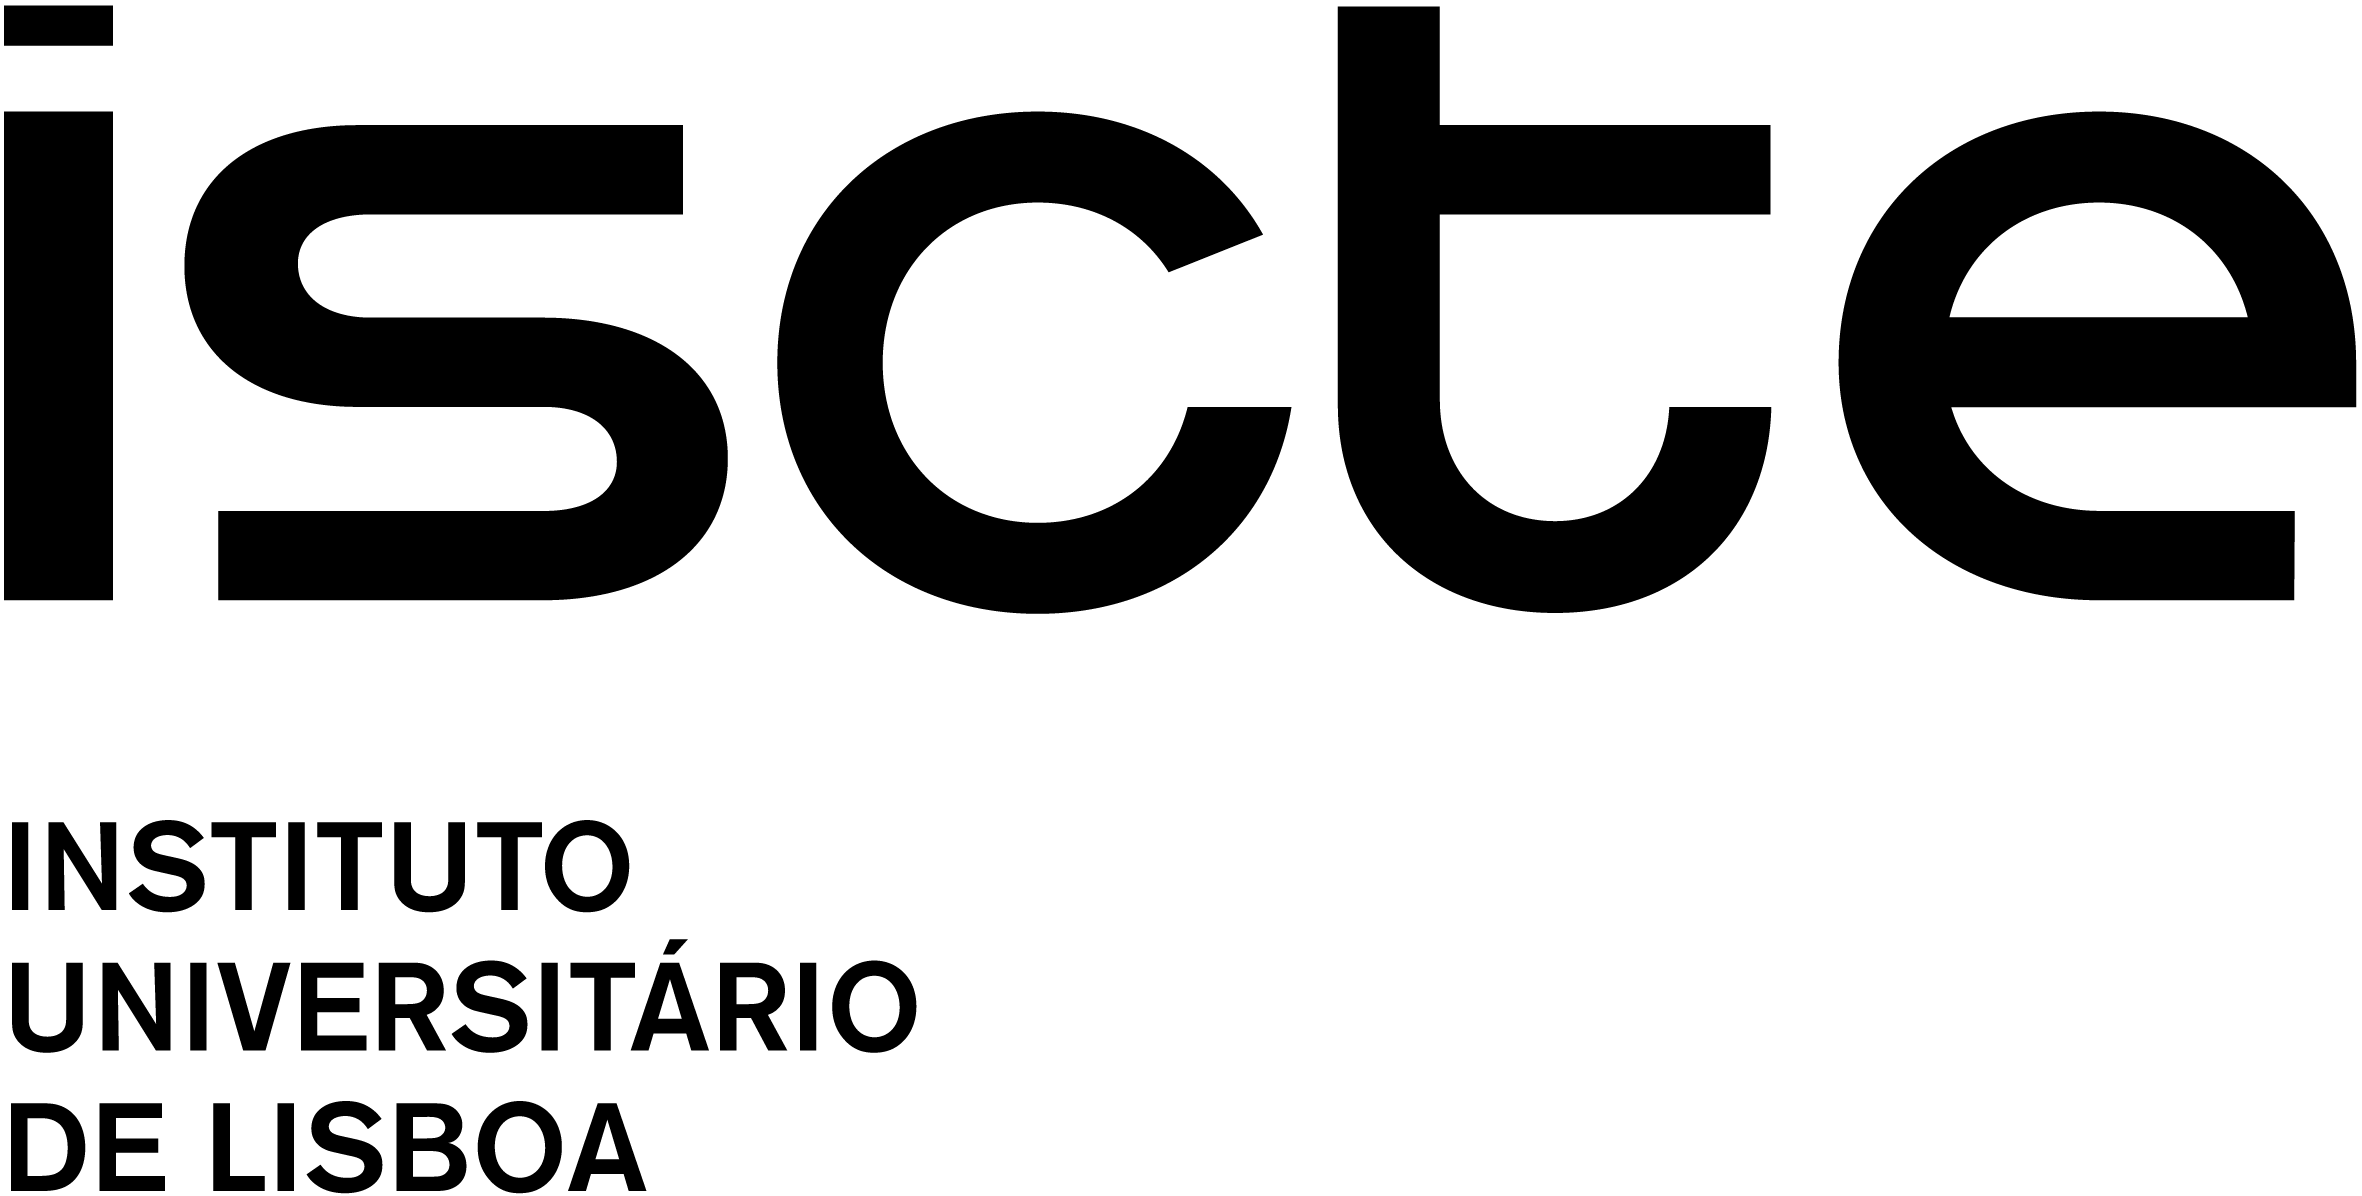
\includegraphics[width=6.03cm]{images/iscte}\\[3.3mm] % DESCOMENTA SE TIVERES IMAGEM
%\textbf{[LOGO ISCTE]}\\[3.3mm]

\hrulefill
~\\
~\\
~\\
% O título ocupa três linhas: quebrado à mão para não deixar o TeX partir
% «Neuroevolução» ou isolar os dois pontos no fim de uma linha.
\textbf{Aprendizagem por Reforço Multiagente e Neuroevolução}\\
\textbf{no Controlo de Enxames de Robôs:}\\
\textbf{Desempenho, Escalabilidade e Robustez}\\
~\\
~\\
~\\
~\\
Gonçalo Alexandre Pombo Santos\\
~\\
~\\
~\\
Mestrado em Inteligência Artificial\\
~\\
~\\
~\\
Orientador:\\
Doutor Luís Miguel Martins Nunes,\\
Professor Associado com Agregação,\\
Iscte-Instituto Universitário de Lisboa\\
~\\
~\\
~\\
%Co-Orientador:\\
%Doutor [Nome], Professor [Categoria],\\
%[Instituição]\\
~\\
~\\
~\\
~\\
setembro, 2026
\end{flushleft}
\thispagestyle{empty}

\cleardoublepage

\begin{flushleft}

\includegraphics[width=6.03cm]{images/ista}\\[7mm] % DESCOMENTA SE TIVERES IMAGEM
%\textbf{[LOGO ISTA]}\\[7mm]
\hrulefill
~\\
~\\
~\\
Departamento de Ciências e Tecnologia da Informação\\
~\\
~\\
% O título ocupa três linhas: quebrado à mão para não deixar o TeX partir
% «Neuroevolução» ou isolar os dois pontos no fim de uma linha.
\textbf{Aprendizagem por Reforço Multiagente e Neuroevolução}\\
\textbf{no Controlo de Enxames de Robôs:}\\
\textbf{Desempenho, Escalabilidade e Robustez}\\
~\\
~\\
~\\
~\\
Gonçalo Alexandre Pombo Santos\\
~\\
~\\
~\\
Mestrado em Inteligência Artificial\\
~\\
~\\
~\\
Orientador:\\
Doutor Luís Miguel Martins Nunes,\\
Professor Associado com Agregação,\\
Iscte-Instituto Universitário de Lisboa\\
~\\
~\\
~\\
%Co-Orientador:\\
%Doutor [Nome], Professor [Categoria],\\
%[Instituição]\\
~\\
~\\
~\\
~\\
setembro, 2026
  \end{flushleft}
  \thispagestyle{empty}
\rmfamily
\normalsize
\frontmatter
\thispagestyle{empty}

\begin{dedication}
\begin{flushright}
\textit{Aos meus pais e a todos que apoiaram este percurso.}
\end{flushright}
\end{dedication}

\setcounter{page}{1}
\pagenumbering{roman}

\chapter*{Agradecimentos}
Gostaria de expressar a minha gratidão aos meus familiares, por me terem apoiado ao longo desta jornada académica, e à minha namorada, por ter estado sempre ao meu lado nos bons e nos maus momentos. Agradeço também aos colegas e amigos que fiz ao longo do tempo, bem como aos professores, por terem dado o seu melhor para nos ensinar. Por fim, agradeço à TAISCTE por ter feito parte deste meu percurso de mestrado.

\vspace{2ex}
\noindent This work was partially supported by national funds through Fundação para a Ciência e a Tecnologia, I.P. (FCT), ISTAR-Iscte Pluriannual Projects UID/04466/2025 (\url{https://doi.org/10.54499/UID/04466/2025}).

\chapter*{Resumo}
Esta dissertação compara a aprendizagem por reforço multiagente e a otimização bio-inspirada no controlo descentralizado de enxames de robôs. Num simulador próprio, vinte robôs têm de chegar em conjunto a um ninho. Um controlador evolutivo, uma rede neuronal sobre grafos com atenção, foi comparado com dois algoritmos de aprendizagem por reforço por gradiente (\textit{Proximal Policy Optimization} e \textit{Soft Actor-Critic}) em sete cenários de dificuldade crescente, com 7 treinos independentes por algoritmo e cenário.

Com uma função de aptidão que premeia também a aproximação ao ninho, o controlador evolutivo supera os métodos de gradiente em três cenários, iguala o melhor noutros dois e é o único que funciona sem novo treino com enxames de 10 a 100 robôs; os métodos de gradiente são mais fiáveis em espaço aberto e gastam menos cálculo. O cenário que obriga a afastar-se do ninho para o alcançar só foi resolvido de forma consistente com pressão por comportamentos novos, atenuada após a descoberta: numa replicação com 28 treinos por algoritmo, resolveu-o em 28, contra 15 sem essa pressão e 14 de cada método de gradiente. Um oitavo cenário, que junta as dificuldades dos sete num labirinto de $103 \times 62$\,m, é resolvido em apenas 4 de 21 treinos.

A hipótese de que a aprendizagem adaptativa supera a otimização estática confirma-se só em parte: escalar depende da representação da política, não do otimizador; nos cenários enganadores, depende do sinal de treino.

\vspace{3ex}
\textsc{Palavras Chave:} Robótica de Enxame, Aprendizagem por Reforço Multiagente, Otimização Bio-inspirada, Redes Neuronais de Grafos.

\chapter*{Abstract}
This dissertation compares multi-agent reinforcement learning and bio-inspired optimization for the decentralized control of robot swarms. In a purpose-built simulator, twenty robots must jointly reach a nest. An evolutionary controller, a graph neural network with attention, was compared with two gradient-based reinforcement learning algorithms (\emph{Proximal Policy Optimization} and \emph{Soft Actor-Critic}) across seven scenarios of increasing difficulty, with 7 independent training runs per algorithm and scenario.

With a fitness function that also rewards approaching the nest, the evolutionary controller outperforms the gradient-based methods in three scenarios, matches the best of them in two others, and is the only one that works without retraining on swarms of 10 to 100 robots; the gradient-based methods are more reliable in open space and need less computation. The scenario that forces the robots to move away from the nest in order to reach it was only solved consistently with pressure towards novel behaviours, attenuated after discovery: in a replication with 28 training runs per algorithm, it solved it in 28, against 15 without that pressure and 14 for each gradient-based method. An eighth scenario, which combines the difficulties of the seven in a $103 \times 62$\,m maze, is solved in only 4 of 21 runs.

The hypothesis that adaptive learning outperforms static optimization is only partly confirmed: scaling depends on the representation of the policy, not on the optimizer; in deceptive scenarios, it depends on the training signal.

\vspace{3ex}
\textsc{Keywords:} Swarm Robotics, Multi-Agent Reinforcement Learning, Bio-inspired Optimization, Graph Neural Networks.

% O índice listava até ao nível `paragraph`: 33 das 144 entradas eram
% parágrafos, e o conjunto transbordava uma ÚNICA linha para uma terceira
% página — «Apêndice D. Recursos Adicionais 115», sozinha, com a página toda
% em branco por baixo. Até `subsection` é o que se pede a um índice de
% dissertação, e o índice fecha em duas páginas.
\setcounter{tocdepth}{2}
\tableofcontents
\listoffigures
\listoftables
\cleardoublepage

\chapter*{Lista de Acrónimos}
\begin{acronym}
 \acro{AABB}{Axis-Aligned Bounding Box}
 \acro{ACO}{Ant Colony Optimization}
 \acro{AE}{Algoritmos Evolutivos}
 \acro{CTDE}{Centralized Training with Decentralized Execution}
 \acro{Dec-POMDP}{Decentralized Partially Observable Markov Decision Process}
 \acro{DQN}{Deep Q-Network}
 \acro{GAE}{Generalized Advantage Estimation}
 \acro{GNN}{Graph Neural Network}
 \acro{MADDPG}{Multi-Agent Deep Deterministic Policy Gradient}
 \acro{MAMDP}{Multi-Agent Markov Decision Process}
 \acro{MAPPO}{Multi-Agent Proximal Policy Optimization}
 \acro{MARL}{Multi-Agent Reinforcement Learning}
 \acro{MDP}{Markov Decision Process}
 \acro{MLP}{Multi-Layer Perceptron}
 \acro{NEAT}{NeuroEvolution of Augmenting Topologies}
 \acro{PBRS}{Potential-Based Reward Shaping}
 \acro{POMDP}{Partially Observable Markov Decision Process}
 \acro{PPO}{Proximal Policy Optimization}
 \acro{PRISMA}{Preferred Reporting Items for Systematic Reviews and Meta-Analyses}
 \acro{PSO}{Particle Swarm Optimization}
 \acro{QI}{Questão de Investigação}
 \acro{QKV}{Query, Key, Value (projeções do mecanismo de atenção)}
 \acro{RL}{Reinforcement Learning}
 \acro{RS2C}{Robust and Scalable Swarm Control}
 \acro{SAC}{Soft Actor-Critic}
 \acro{SI}{Swarm Intelligence}
 \acro{SLAM}{Simultaneous Localization and Mapping}
 \acro{SLR}{Systematic Literature Review}
 \acro{SR}{Swarm Robotics}
% O acronym acrescenta um \item[] vazio quando nenhum acrónimo foi «usado» com
% \ac{} — e a tese não usa \ac{} —, o que imprimia um «:» solto no fim da lista.
\makeatletter\global\let\AC@populated\AC@used\makeatother
\end{acronym}

\mainmatter
\setcounter{page}{1} \pagenumbering{arabic}
\acresetall

% --- CAPÍTULO 1 ---
\chapter{Introdução}

\section{Enquadramento e Motivação}
A robótica de enxame (\textit{Swarm Robotics}) estuda a coordenação de grandes grupos de robôs simples, sem controlo central, a partir de interações locais \cite{bonabeau1999swarm}. A premissa é que o comportamento útil do grupo não exige complexidade em cada membro: resulta das interações entre eles. Tegmark defende uma ideia próxima, a de que a inteligência é, no essencial, processamento de informação, em larga medida independente do substrato físico \cite{tegmark2017life}. Desde os primeiros trabalhos, no início da década de 1990, a motivação do campo mantém-se: reproduzir a inteligência coletiva observada na natureza, em colónias de formigas ou em cardumes, para obter sistemas robustos, flexíveis e escaláveis \cite{dorigo1992optimization, kennedy1995pso}.

Estes sistemas interessam sobretudo a aplicações em ambientes incertos ou perigosos, como a vigilância de infraestruturas, a exploração espacial ou a resposta a desastres naturais \cite{ekechi2025survey}. Nesses cenários, a redundância do enxame é a principal vantagem: a perda de um agente não deve comprometer a missão \cite{pina2024self}.

A dificuldade está no controlo. Métodos que dependem de uma unidade central ou de um modelo global do sistema escalam mal com o número de agentes ($N$). Parte da dificuldade é o que se conhece como \emph{complexidade combinatória} (\textit{combinatorial complexity}): o espaço conjunto de estados e ações cresce exponencialmente com o número de agentes, o que torna impraticável programar à mão todas as situações \cite{majid2023deep}. Hüttenrauch et al. (2019) argumentam que, para escalar, a política de controlo tem de ser independente do número total de agentes \cite{huttenrauch2019deep}.

Para desenhar estes controladores descentralizados, a literatura segue sobretudo duas abordagens, que não são as únicas mas são as que este trabalho compara:

\begin{enumerate}
    \item \textbf{Otimização Bio-inspirada:} Métodos como o \textit{Particle Swarm Optimization} (PSO) e Algoritmos Evolutivos (AE) focam-se na robustez \textit{offline} \cite{kennedy1995pso}. Tratam o desenho do controlador como um problema de otimização estocástica, procurando os pesos ótimos de uma rede neuronal ou parâmetros de regras heurísticas antes da implantação real \cite{hassen2025hybrid, salimans2017es}. Embora robustos, estes métodos tendem a ser estáticos, podendo carecer de adaptabilidade perante mudanças dinâmicas e imprevistas no ambiente \cite{somvanshi2025influx}.
    \item \textbf{Multi-Agent Reinforcement Learning (MARL):} Focado na adaptabilidade \textit{online}, o MARL utiliza o paradigma de aprendizagem sequencial para que os agentes descubram políticas cooperativas através da interação direta com o ambiente \cite{sutton2018reinforcement}. O problema formaliza-se como um \textit{Decentralized Partially Observable Markov Decision Process} (Dec-POMDP), e o que o MARL promete é aprender políticas que reagem ao que cada agente observa, em vez de seguirem um plano fixo \cite{huh2023marl}.
\end{enumerate}

A pertinência desta investigação sustenta-se na escassez de estudos que comparem diretamente a eficiência e a robustez destas duas escolas em cenários operacionais dinâmicos, que a revisão sistemática do Capítulo~\ref{ch:sota} documenta. Majid et al. (2024) comparam as duas famílias no plano conceptual --- as estratégias evolutivas tendem a produzir políticas mais robustas, mas são ainda menos eficientes em amostras do que a aprendizagem por reforço --- e apontam a sua hibridização como promissora, sem as confrontar experimentalmente \cite{majid2023deep}. Esta dissertação compara as duas famílias nas mesmas condições, quanto a desempenho, escalabilidade e robustez.

\section{Definição do Problema e Justificação da Tese}
Falta na literatura uma comparação direta (\textit{benchmarking}) do desempenho de paradigmas concorrentes em cenários de controlo de enxames que sejam, simultaneamente, complexos e dinâmicos --- de que é sintoma a própria \textit{suite} de referência do MARL não incluir qualquer \textit{baseline} evolutiva \cite{bettini2024benchmarl}. Na literatura revista no Capítulo~\ref{ch:sota}, embora existam múltiplos \textit{frameworks} de controlo, a maioria dos estudos avalia um único paradigma, sem a validação cruzada necessária para determinar a aplicabilidade de cada método.

O \textit{Multi-Agent Reinforcement Learning} (MARL), embora capaz de aprender comportamentos coletivos complexos, enfrenta dificuldades conhecidas. Entre estas, destaca-se a \emph{não-estacionaridade} do ambiente: como todos os agentes aprendem e alteram as suas políticas simultaneamente, a dinâmica do sistema do ponto de vista de um agente individual muda constantemente, violando a propriedade de Markov necessária para a convergência de algoritmos tradicionais \cite{huh2023marl}. Além disso, a explosão do espaço de ações conjuntas em enxames de grande escala dificulta a estabilidade do treino e a otimização de funções de recompensa esparsas.

Por outro lado, os métodos evolutivos e bio-inspirados (como o PSO) têm demonstrado uma robustez consolidada, tratando o controlo como a exploração de uma superfície de \textit{fitness} global \cite{kennedy1995pso}. Contudo, o controlador que resulta da otimização \textit{offline} fica fixo após a implantação: não continua a adaptar-se perante mudanças estruturais imprevistas no ambiente. A isto soma-se o que Kegeleirs e Birattari (2025) designam por \textit{Deployment Gap} (fosso de implantação) --- a ausência de garantia de que um controlador desenvolvido em simulação, ou numa plataforma, mantenha a eficácia quando aplicado noutra ---, a par do \textit{reality gap}, que os autores apontam como preocupação central sobretudo na abordagem evolutiva \cite{kegeleirs2025towards}.

O problema desta dissertação é, portanto, fazer essa comparação de forma sistemática, em três eixos:

\begin{itemize}
    \item \textbf{Desempenho da Tarefa:} Medir a eficácia na concretização do objetivo coletivo --- a taxa de sucesso e o número de chegadas cooperativas ao ninho --- e o custo computacional que cada paradigma paga para lá chegar.
    \item \textbf{Escalabilidade (Zero-Shot Transfer):} Analisar como a \textit{performance} se degrada à medida que o número de agentes ($N$) aumenta para além do cenário de treino. Interessa verificar se a representação por \textit{Graph Neural Networks} (GNNs) --- cujo mecanismo de invariância à cardinalidade é caracterizado por Chen et al. (2024) \cite{chen2024graph}, ainda que no domínio das redes sem fios --- permite uma escalabilidade superior à das políticas de dimensão de entrada fixa (MLP) usadas pelas \textit{baselines} de gradiente. Note-se que, neste trabalho, é o controlador \emph{evolutivo} que instancia a arquitetura de grafo: o eixo da escalabilidade opõe, portanto, representações (grafo \textit{vs.}\ vetor fixo) e não paradigmas de otimização.
    \item \textbf{Robustez a Falhas:} Testar a resiliência do sistema perante a perda súbita de agentes (falhas de \textit{hardware}) a meio da tarefa. Em ambos os paradigmas a política fica fixa depois do treino, pelo que o que se mede é a tolerância a falhas do comportamento aprendido, e não uma adaptação durante a execução.
\end{itemize}

O objetivo prático é dar a quem desenha um enxame dados quantitativos para escolher o paradigma de controlo em função dos requisitos da missão e do cómputo disponível.

\section{Objetivos da Tese}
O objetivo geral desta dissertação é \emph{desenvolver um simulador de enxames e comparar, nas mesmas condições, o \textit{Multi-Agent Reinforcement Learning} (MARL) com a otimização bio-inspirada} (em concreto, a neuroevolução) no controlo descentralizado de enxames. Pretende-se determinar, de forma quantitativa, em que condições cada paradigma é preferível.

Para atingir o objetivo geral, foram definidos os seguintes objetivos específicos:
\begin{itemize}
    \item \textbf{Desenvolver um Ambiente de Simulação Abrangente:} Projetar e implementar um simulador em ambiente Python capaz de modelar tarefas fundamentais de enxame, como a navegação cooperativa até um ninho móvel e a perceção cooperativa (cerco de alvos móveis), em cenários de dificuldade de navegação crescente. O ambiente deve contemplar colisões e deslizamento nas paredes, perceção do ambiente por sensores de alcance limitado e a simulação de falhas súbitas de agentes para testar a resiliência do sistema \cite{pina2024self}.
    \item \textbf{Implementar um Framework MARL (RS2C):} Desenvolver o \textit{framework} \textit{Robust and Scalable Swarm Control} (RS2C), assente em execução descentralizada com partilha de parâmetros, sobre as implementações de referência do PPO e do SAC.
    \item \textbf{Implementar uma \textit{Baseline} de Otimização Bio-inspirada:} Desenvolver um controlador baseado em \emph{Neuroevolução} (um Algoritmo Evolutivo, AE) para servir de termo de comparação de desempenho \cite{such2017deep, salimans2017es}. Este controlador é otimizado \textit{offline}, sem gradientes, para encontrar os pesos de uma rede neuronal de grafos com atenção, cuja invariância à permutação permite aplicar um controlador treinado com $N$ agentes a enxames de outra dimensão sem retreino (\textit{Zero-Shot Transfer}) \cite{such2017deep}.
    \item \textbf{Realizar uma Análise Comparativa e Estatística:} Executar experiências controladas com as métricas de desempenho da tarefa, escalabilidade e robustez a falhas. Os resultados deverão ser validados estatisticamente --- testes de hipótese não-paramétricos sobre execuções de treino independentes, complementados por medidas de tamanho de efeito ---, garantindo que as conclusões sobre a superioridade de um paradigma sobre o outro são cientificamente sustentadas.
\end{itemize}

\section{Questões de Investigação}
\label{sec:questoes_investigacao}
Decorrentes da definição do problema e dos três eixos de avaliação enunciados (desempenho, escalabilidade e robustez), a investigação organiza-se em \emph{dois níveis}. O primeiro é o da comparação entre paradigmas: quatro questões gerais, que interrogam o que cada família de métodos consegue e em que condições. O segundo desce ao nível dos \emph{mecanismos} que produzem esse desempenho --- três questões deliberadamente mais específicas, cada uma isolando um fator que a comparação de primeiro nível agrega: o desenho do sinal de treino, a pressão de exploração e a topologia do ambiente. A \emph{hipótese central} que as atravessa é a de que a \emph{inteligência adaptativa} (MARL) supera a \emph{robustez estática} bio-inspirada no controlo de enxames; é validada na Secção~\ref{sec:res_discussao}, e todas as questões são retomadas explicitamente nas Conclusões (Secção~\ref{sec:resposta_qi}).

\paragraph{Nível 1 --- Questões gerais: a comparação entre paradigmas.}
\begin{enumerate}
    \item[\textbf{QI1.}] \textbf{Desempenho de tarefa:} Qual dos paradigmas de controlo descentralizado --- MARL por gradiente (PPO/SAC) ou neuroevolução --- atinge maior eficácia nas tarefas coletivas avaliadas --- navegação cooperativa até ao ninho e perceção cooperativa de alvos móveis ---, em cenários de dificuldade de navegação e de coordenação crescente?
    \item[\textbf{QI2.}] \textbf{Escalabilidade (\textit{Zero-Shot Transfer}):} Uma política treinada com $N=20$ agentes transfere-se, sem retreino, para enxames de dimensão distinta ($N=10$ a $N=100$)? Em que medida essa capacidade depende da arquitetura da política (rede de grafos com atenção vs.\ MLP de dimensão fixa)?
    \item[\textbf{QI3.}] \textbf{Robustez a falhas:} Como se degrada o desempenho coletivo de cada paradigma perante a falha súbita de uma fração dos agentes durante a execução da tarefa?
    \item[\textbf{QI4.}] \textbf{Critério de escolha:} Em que condições operacionais (tipo de cenário, dimensão do enxame, requisitos de fiabilidade) se justifica preferir um paradigma ao outro?
\end{enumerate}

\paragraph{Nível 2 --- Questões específicas: os mecanismos por detrás do desempenho.}
As três questões seguintes decorrem das anteriores e só se tornam formuláveis depois delas: cada uma toma um resultado do primeiro nível e pergunta \emph{de que} é que ele depende. São, por isso, mais estreitas --- e é essa estreiteza que as torna testáveis com uma experiência controlada.

\begin{enumerate}
    \item[\textbf{QI5.}] \textbf{Desenho da função de \textit{fitness}} (aprofunda a QI1)\textbf{:} Em que medida o desempenho do controlador neuroevolutivo depende do desenho da função de \textit{fitness}? Em particular, pode um \textit{shaping} de navegação (\textit{homing}), que premeia a aproximação ao objetivo antes da primeira chegada, desbloquear cenários que uma \textit{fitness} de tarefa pura não resolve?
    \item[\textbf{QI6.}] \textbf{Deceção e procura por novidade} (aprofunda a QI1 e a QI5)\textbf{:} Em cenários cujo gradiente de recompensa é enganador (\textit{deceptive}), a hibridização da neuroevolução com procura por novidade (\textit{Novelty Search}) melhora o resultado final face à otimização puramente objetiva?
% ── QI7: a PERGUNTA, não a resposta. Esteve aqui em comentário desde 6 de
% agosto, à espera de a secção do mapa grande entrar, e foi descomentada a 17.
% ⚠️ Ficou então ANTES da QI6, porque era aí que o bloco em comentário estava —
% a lista lia-se 1, 2, 3, 4, 5, 7, 6. Reposta na ordem a 18 de agosto.
    \item[\textbf{QI7.}] \textbf{Composição de dificuldades} (aprofunda a QI1 e a QI4)\textbf{:} As conclusões
         obtidas em sete cenários de dificuldade isolada transferem-se para um
         ambiente que \emph{combina} essas dificuldades a uma escala
         substancialmente maior, ou a composição faz emergir modos de falha que
         os cenários isolados não revelam?
\end{enumerate}

\section{Estrutura do Documento}
\label{sec:estrutura_documento}
Além desta Introdução, o documento organiza-se em seis capítulos e cinco anexos:
\begin{itemize}
    \item O \textbf{Capítulo~\ref{ch:fundamentos}} apresenta os fundamentos teóricos dos dois paradigmas comparados --- os algoritmos evolutivos, os processos de decisão de Markov e os algoritmos PPO e SAC --- e das redes de grafos com atenção em que assenta o controlador neuroevolutivo.
    \item O \textbf{Capítulo~\ref{ch:sota}} reporta a revisão sistemática da literatura: o protocolo seguido, a caracterização dos estudos incluídos, o problema da transferência da simulação para robôs reais e as lacunas a que esta dissertação responde.
    \item O \textbf{Capítulo~\ref{ch:simulation_env}} descreve o simulador desenvolvido --- arquitetura de software, modelo físico, observações e ações dos agentes, os sete cenários de teste e a função de recompensa --- e a estrutura do projeto.
    \item O \textbf{Capítulo~\ref{ch:algorithms}} detalha os controladores comparados (o \textit{framework} RS2C, com PPO e SAC, e o controlador neuroevolutivo, com a sua função de aptidão e a procura por novidade) e o plano experimental e estatístico.
    \item O \textbf{Capítulo~\ref{ch:results}} apresenta e discute os resultados: desempenho por cenário, fiabilidade entre execuções, deceção e procura por novidade, o oitavo cenário composto, escalabilidade, robustez a falhas e custo computacional.
    \item O \textbf{Capítulo~\ref{ch:conclusoes}} responde às questões de investigação e declara as limitações, os contributos e os trabalhos futuros.
\end{itemize}
Os anexos reúnem a declaração de utilização de ferramentas de inteligência artificial (Anexo~\ref{apx:ia}), as configurações e hiperparâmetros (Anexo~\ref{apx:hyperparameters}), os estudos incluídos na revisão sistemática (Anexo~\ref{apx:slr}), o diagrama de classes e os excertos de código mais relevantes (Anexo~\ref{apx:code}) e a localização do repositório com o código e os dados (Anexo~\ref{apx:resources}).

% --- CAPÍTULO 2 ---
\chapter{Fundamentos Teóricos e Tecnologias}
\label{ch:fundamentos}

\section{Introdução ao Capítulo}
Este capítulo apresenta os conceitos e a notação usados no resto da dissertação: a inteligência e a robótica de enxame, os dois paradigmas de controlo comparados e as redes de grafos com atenção.

Começa-se pelos conceitos de \textit{Swarm Intelligence} (SI) e \textit{Swarm Robotics} (SR), que explicam como comportamentos globais podem emergir de regras locais simples. A descentralização que torna estes sistemas robustos também dificulta o desenho dos controladores: como mostram Rivière et al. (2020), sintetizar políticas que operem apenas sobre o estado relativo dos vizinhos próximos --- e que ainda assim aproximem o desempenho de um planeador global --- é, em si mesmo, um problema de investigação em aberto \cite{riviere2020glas}.

Seguem-se os dois paradigmas de controlo que esta dissertação compara:
\begin{enumerate}
    \item \textbf{Otimização Bio-inspirada:} Serão explorados algoritmos como a Otimização por Enxame de Partículas (\textit{Particle Swarm Optimization} - PSO) e os Algoritmos Evolutivos (AE). Estas técnicas tratam o controlo como um problema de busca num espaço de parâmetros global, focando-se na convergência para soluções estáveis e robustas em cenários estáticos.
    \item \textbf{Multi-Agent Reinforcement Learning (MARL):} Será introduzida a formalização matemática do problema através do modelo de Processo de Decisão de Markov Parcialmente Observável Descentralizado (\textit{Dec-POMDP}). Descreve-se como a aprendizagem por reforço aprende políticas por interação com o ambiente, bem como a arquitetura \textit{Centralized Training with Decentralized Execution} (CTDE) e o papel das \textit{Graph Neural Networks} (GNNs) na garantia da escalabilidade do enxame, tal como defendido por Chen et al. (2024).
\end{enumerate}

A transferência destes controladores da simulação para robôs reais --- o \textit{Deployment Gap} de Kegeleirs e Birattari (2025) --- é tratada no capítulo seguinte (Secção~\ref{sec:deployment_gap}) \cite{kegeleirs2025towards}.

\section{Swarm Intelligence (SI) e Robótica de Enxame}
A Inteligência de Enxame (\textit{Swarm Intelligence} - SI) refere-se ao comportamento coletivo e coordenado de sistemas descentralizados e auto-organizados, sejam eles naturais ou artificiais \cite{dorigo1992optimization}. Este paradigma baseia-se na observação de sistemas biológicos — tais como colónias de formigas, enxames de abelhas ou cardumes de peixes — onde agentes individuais com capacidades cognitivas limitadas conseguem, através de interações sociais simples, resolver problemas de elevada complexidade que excederiam a capacidade de qualquer indivíduo isolado \cite{kennedy1995pso}.

A Robótica de Enxame (\textit{Swarm Robotics} - SR) surge como a aplicação direta dos princípios de SI ao domínio de sistemas multi-robô \cite{bonabeau1999swarm}. Ao contrário da robótica cooperativa tradicional, a SR foca-se na coordenação de um grande número de agentes, tipicamente homogéneos e de baixo custo, que operam sem uma infraestrutura de controlo centralizada ou um mapa global do ambiente. O controlo nestes sistemas é inerentemente distribuído, o que confere ao coletivo três propriedades fundamentais identificadas na literatura:
\begin{itemize}
    \item \textbf{Robustez:} A redundância do sistema garante que a missão prossiga mesmo perante a falha de múltiplos agentes \cite{huttenrauch2019deep}.
    \item \textbf{Escalabilidade:} O sistema mantém a sua eficiência independentemente da dimensão do enxame ($N$), uma vez que as interações são predominantemente locais.
    \item \textbf{Flexibilidade:} O enxame consegue adaptar-se a diferentes tarefas e ambientes dinâmicos sem necessidade de reprogramação externa.
\end{itemize}

O alicerce técnico destes sistemas reside no comportamento emergente. Conforme sistematizado por Bonabeau, Dorigo e Theraulaz (1999) no estudo dos insetos sociais, as ações globais coordenadas emergem de um ciclo de \textit{feedback} contínuo entre regras de interação locais simples e o ambiente \cite{bonabeau1999swarm}. Um mecanismo crítico para esta emergência é a \emph{estigmergia}, um método de coordenação indireta onde os agentes alteram o ambiente (por exemplo, depositando trilhos de feromonas), influenciando as ações subsequentes de outros membros do grupo --- o princípio que está na origem da própria Otimização por Colónias de Formigas \cite{dorigo1992optimization}.

No entanto, projetar manualmente estas regras locais para atingir um objetivo global específico é um desafio de engenharia não trivial. Como não existe um ``conhecimento global'' partilhado, o desenho do controlador deve garantir que a soma das micro-decisões individuais resulte na macro-estabilidade do enxame. É isso que motiva o recurso à aprendizagem automática: em vez de programar as regras à mão, o sistema aprende-as por reforço ou fá-las evoluir por otimização.

\section{Paradigmas de Controlo para Enxames}
O controlo de sistemas multi-robô em larga escala foca-se primordialmente no desenho das chamadas ``regras locais'' de interação. O desafio fundamental reside na resolução do problema inverso da robótica de enxame: como determinar comportamentos individuais simples que, quando executados em paralelo, resultem numa macro-estabilidade e no cumprimento de um objetivo global. De entre as várias famílias de métodos propostas para o efeito, destacam-se na literatura contemporânea duas abordagens dominantes \cite{majid2023deep, kegeleirs2025towards, bredeche2022social} --- que não esgotam o espaço de soluções, mas concentram o essencial do debate atual --- e são estas que esta tese se propõe a analisar e comparar:

\begin{enumerate}
    \item \textbf{Otimização Bio-inspirada (Offline):} Esta categoria abrange duas subfamílias principais frequentemente utilizadas em robótica:
    \begin{itemize}
        \item \textbf{Algoritmos Evolutivos (AE):} Inspirados na seleção natural (Darwin), utilizam operadores como mutação e cruzamento para evoluir uma população de controladores ao longo de gerações.
        \item \textbf{Inteligência de Enxame (SI):} Inspirados em comportamentos sociais (e.g., bandos de pássaros), como o \textit{Particle Swarm Optimization} (PSO), onde a solução emerge do movimento cooperativo de partículas no espaço de busca.
    \end{itemize}
    Ambas as abordagens procuram \textit{offline} o melhor conjunto de parâmetros fixos, maximizando uma função de \textit{fitness}. Embora gerem comportamentos robustos, resultam frequentemente em controladores rígidos perante mudanças ambientais não previstas.

    \item \textbf{Aprendizagem por Reforço (Online/Adaptativa):} Em vez de otimizar parâmetros fixos antes da implantação, o agente aprende uma política $\pi(a \mid o)$ através da interação sequencial com o ambiente, guiado por um sinal de recompensa. Na sua extensão multiagente (MARL), cada robô ajusta o seu comportamento em função das observações locais, permitindo em princípio a adaptação a condições não previstas no desenho. O custo desta flexibilidade é uma otimização substancialmente mais difícil: a não-estacionaridade introduzida pela aprendizagem simultânea de todos os agentes, a atribuição de crédito em recompensas coletivas e a sensibilidade ao desenho do sinal de recompensa (Secção~\ref{sec:reward_design}) são desafios centrais que esta tese aborda empiricamente.
\end{enumerate}

É esta distinção que a comparação explora: permite avaliar se o custo computacional e a complexidade de treino da aprendizagem automática são justificados por um ganho real em adaptabilidade face às soluções otimizadas tradicionais.

\section{Abordagem 1: Otimização Bio-inspirada}
Esta abordagem utiliza algoritmos de busca meta-heurística para navegar no vasto espaço de parâmetros $\theta$ de um controlador — frequentemente representado por uma rede neuronal (\textit{Neuroevolution}) ou uma máquina de estados — com o intuito de maximizar uma função de desempenho global $J(\theta)$.

\subsection{Fundamentos Matemáticos dos Algoritmos Evolutivos}
\label{sec:fundamentos_ae}
O processo evolutivo opera sobre uma \emph{população} $\Pi_g = \{\theta_1, \theta_2, \ldots, \theta_K\}$ de $K$ controladores candidatos, denominados \emph{genomas}, onde cada genoma $\theta_k \in \mathbb{R}^{|\theta|}$ é o vetor concatenado de todos os pesos e \textit{biases} de uma rede neuronal. A topologia arquitetural da rede é fixada \textit{a priori}; apenas os seus parâmetros numéricos são sujeitos a otimização --- esta abordagem denomina-se \emph{Neuroevolução}. Ao contrário do RL, a Neuroevolução não necessita de gradientes calculáveis, tornando-a aplicável a qualquer função de recompensa não-diferenciável.

\paragraph{O ciclo evolutivo:}
Um algoritmo evolutivo itera três operações sobre a população: \emph{avaliação} --- atribuir a cada genoma um valor de aptidão $J(\theta_k)$, obtido executando o controlador correspondente no ambiente ---, \emph{seleção} --- reter os genomas de maior aptidão --- e \emph{variação} --- gerar descendentes por mutação e, nalgumas formulações, por recombinação. A geração $g+1$ é, assim, uma amostra enviesada para as regiões de $\mathbb{R}^{|\theta|}$ que a geração $g$ mostrou serem promissoras. Como a única informação utilizada é a \emph{ordenação} das aptidões, o método aplica-se a funções não-diferenciáveis, descontínuas ou avaliáveis apenas por simulação --- é esta propriedade que o torna atrativo em robótica de enxame, onde o desempenho coletivo raramente admite gradiente analítico \cite{majid2023deep, bredeche2022social}.

\paragraph{Função de aptidão (\textit{fitness}):}
A função $J(\theta_k)$ é o único canal por onde o objetivo do projetista entra na otimização, e a literatura mostra que a sua formulação condiciona o resultado tanto quanto o algoritmo de busca. Uma aptidão que meça apenas o objetivo final tende a ser \emph{esparsa} --- nenhum genoma da população inicial se distingue dos restantes ---, ao passo que uma aptidão enriquecida com termos intermédios (\textit{shaping}) corre o risco de se tornar \emph{enganadora} (\textit{deceptive}), premiando comportamentos que afastam da solução. É esta tensão que motiva alternativas como a procura por novidade, que substitui parcialmente a pressão pelo objetivo por pressão pela diversidade comportamental \cite{lehman2011abandoning, hasselmann2023novelty}.

\paragraph{Operadores de variação:}
Em neuroevolução de topologia fixa, o operador canónico é a \emph{mutação gaussiana} (\textit{Gaussian mutation}): cada descendente resulta de perturbar o vetor de pesos do progenitor,
\begin{equation}
    \theta^{(\text{filho})} = \theta^{(\text{pai})} + \boldsymbol{\varepsilon}, \qquad \boldsymbol{\varepsilon} \sim \mathcal{N}(\mathbf{0}, \sigma^2 \mathbf{I}),
    \label{eq:mutacao_gaussiana}
\end{equation}
onde $\mathcal{N}(\boldsymbol{\mu}, \boldsymbol{\Sigma})$ denota a distribuição normal de média $\boldsymbol{\mu}$ e covariância $\boldsymbol{\Sigma}$, $\mathbf{I}$ é a matriz identidade e $\sigma$, o \emph{passo de mutação} (\textit{mutation step size}), fixa a escala da perturbação. Salimans et al.\ mostram que esta forma de busca, paralelizada por muitos trabalhadores, é competitiva com a aprendizagem por reforço em tarefas de controlo contínuo \cite{salimans2017es}. Uma variante frequente perturba apenas um subconjunto aleatório das coordenadas, para preservar diversidade em espaços de grande dimensão. Uma família distinta --- \textit{NeuroEvolution of Augmenting Topologies} (NEAT) e derivados --- evolui também a \emph{topologia} da rede, e não apenas os seus pesos, ao custo de um espaço de busca substancialmente mais complexo \cite{zaman2025neat, biteng2025training}.

\paragraph{Controlo do passo de mutação:}
O valor de $\sigma$ arbitra entre exploração e refinamento: valores elevados amostram regiões distantes do espaço de pesos, valores baixos afinam o ótimo já encontrado. É prática corrente fazê-lo decair ao longo das gerações --- por analogia com a \emph{temperagem} (\textit{annealing}) da metalurgia ---, tipicamente de forma geométrica e com um patamar mínimo que impede o colapso da diversidade:
\begin{equation}
    \sigma_{g+1} = \max\!\left(\sigma_{\min},\; \sigma_g \cdot \rho\right), \qquad 0 < \rho < 1
    \label{eq:sigma_decay}
\end{equation}
onde $g$ indexa a geração, $\rho$ é o \emph{fator de decaimento} e $\sigma_{\min}$ o patamar mínimo do passo de mutação.

\paragraph{Seleção e elitismo:}
A seleção por \emph{truncatura} (\textit{truncation selection}) ordena a população por aptidão e descarta a cauda inferior; o \emph{elitismo} (\textit{elitism}) copia intactos os melhores genomas para a geração seguinte, garantindo que o melhor comportamento descoberto nunca se perde por uma mutação desfavorável --- propriedade que torna a melhor aptidão monótona não-decrescente ao longo das gerações. Em robótica de enxame estas escolhas convivem com uma dificuldade adicional: a aptidão é estimada por simulação estocástica, pelo que um genoma pode ser selecionado por ter tido sorte na avaliação e não por ser efetivamente melhor --- razão pela qual se avalia cada genoma em vários episódios e se fixam as \textit{seeds} de avaliação \cite{bredeche2022social, fontbonne2020online}.

\paragraph{Otimização por Enxame de Partículas (PSO):} O PSO modela cada controlador candidato como uma ``partícula'' que navega num espaço de busca multidimensional. A inovação crucial deste método reside na partilha de informação social: cada partícula ajusta a sua velocidade e posição baseada na sua melhor experiência pessoal ($pBest$) e na melhor experiência coletiva descoberta por todo o enxame ($gBest$). Hassen e Amin (2025) empregam o PSO para a otimização global do percurso, delegando a reação a obstáculos imprevistos num controlador reativo separado (\textit{Dynamic Window Approach}) --- arranjo que ilustra a característica estrutural do paradigma: a convergência do enxame produz um controlador \emph{estático}, de elevada qualidade para o problema otimizado, mas cuja adaptação ao imprevisto tem de ser acrescentada por fora \cite{hassen2025hybrid}.

A instanciação concreta destes elementos no controlador desta dissertação --- a função de aptidão adotada, a forma da mutação, os valores de $\sigma$ e a dimensão da elite --- é matéria do Capítulo~\ref{ch:algorithms} (Secção~\ref{sec:algo_evolutivo}), e não deste.

\section{Abordagem 2: Multi-Agent Reinforcement Learning (MARL)}
O MARL aplica a aprendizagem por reforço a sistemas com vários agentes, que aprendem políticas ($\pi$) por interação sequencial com o ambiente.

\subsection{Processos de Decisão de Markov (MDPs) e Dec-POMDP}
\label{sec:fund_mdp}
\paragraph{Fundamentos do Processo de Decisão de Markov (MDP):}
A base matemática da aprendizagem por reforço é o \emph{Processo de Decisão de Markov (MDP)}, definido pela tupla $\langle \mathcal{S}, \mathcal{A}, \mathcal{P}, \mathcal{R}, \gamma \rangle$:
\begin{itemize}
    \item $\mathcal{S}$: espaço de estados do ambiente (contínuo em robótica);
    \item $\mathcal{A}$: espaço de ações --- discreto ou contínuo; em robótica móvel é tipicamente um vetor de comando contínuo e limitado;
    \item $\mathcal{P}(s'\mid s,a)$: dinâmica de transição --- probabilidade de atingir $s'$ ao executar $a$ em $s$;
    \item $\mathcal{R}(s,a,s') \in \mathbb{R}$: sinal de recompensa escalar;
    \item $\gamma \in [0,1)$: fator de desconto temporal, que pondera as recompensas futuras face às imediatas.
\end{itemize}

A instanciação concreta desta tupla no ambiente desta dissertação --- a forma e a escala do vetor de ação, o sinal de recompensa e os valores dos hiperparâmetros --- é matéria do Capítulo~\ref{ch:simulation_env} e da Secção~\ref{sec:algo_rl}, e não deste.

\paragraph{Funções de Valor e Equação de Bellman:}
O objetivo do agente é encontrar uma política $\pi^*(a\mid s)$ que maximize o \emph{retorno esperado descontado} (\textit{expected discounted return}) $G_t = \sum_{k=0}^{\infty} \gamma^k r_{t+k}$, em que $r_t$ é a recompensa escalar recebida no instante $t$. A qualidade de uma política é quantificada por duas funções fundamentais.

A \emph{Função de Valor de Estado} (\textit{State-Value Function}) $V^\pi(s)$ mede o retorno esperado ao seguir $\pi$ a partir de $s$:
\begin{equation}
    V^\pi(s) = \mathbb{E}_\pi\!\left[\sum_{t=0}^{\infty} \gamma^t r_t \;\Big|\; s_0 = s\right]
    \label{eq:value_function}
\end{equation}

A \emph{Função $Q$} (ou Função de Valor de Ação, \textit{Action-Value Function}) $Q^\pi(s,a)$ mede o retorno esperado ao executar $a$ em $s$ e depois seguir $\pi$:
\begin{equation}
    Q^\pi(s,a) = \mathbb{E}_\pi\!\left[\sum_{t=0}^{\infty} \gamma^t r_t \;\Big|\; s_0 = s,\, a_0 = a\right]
    \label{eq:q_function}
\end{equation}

Estas funções satisfazem a \emph{Equação de Bellman}, que permite a sua estimação recursiva:
\begin{equation}
    V^\pi(s) = \sum_{a} \pi(a\mid s) \sum_{s'} \mathcal{P}(s'\mid s,a)\!\left[\mathcal{R}(s,a,s') + \gamma V^\pi(s')\right]
    \label{eq:bellman}
\end{equation}

A política ótima verifica a \emph{Equação de Bellman de Optimalidade} (\textit{Bellman Optimality Equation}):
\begin{equation}
    Q^*(s,a) = \mathbb{E}_{s'}\!\left[\mathcal{R}(s,a,s') + \gamma \max_{a'} Q^*(s',a')\right]
    \label{eq:bellman_optimal}
\end{equation}

\paragraph{Extensão para Dec-POMDP em Enxames:}
Em sistemas multiagente, o estado global $s \in \mathcal{S}$ é inacessível a qualquer robô individual. O problema estende-se para o \emph{Processo de Decisão de Markov Parcialmente Observável Descentralizado (Dec-POMDP)}, definido pela tupla $\langle \mathcal{N}, \mathcal{S}, \{\mathcal{A}_i\}_{i \in \mathcal{N}}, \mathcal{P}, \mathcal{R}, \Omega, \{\mathcal{O}_i\}_{i \in \mathcal{N}}, \gamma \rangle$, onde $\mathcal{N} = \{1,\ldots,N\}$ é o conjunto de agentes, $\Omega$ é o espaço de observações conjuntas, e $o_i = \mathcal{O}_i(s) \in \mathbb{R}^{111}$ é a observação local e parcial do agente $i$ (o caligráfico $\mathcal{N}$ designa aqui o conjunto de agentes; a distribuição normal escreve-se com os seus parâmetros, $\mathcal{N}(\boldsymbol{\mu}, \boldsymbol{\Sigma})$) \cite{oliehoek2016concise, sutton2018reinforcement, huh2023marl}. Cada robô mantém uma política descentralizada $\pi_i(a_i \mid o_i)$ e o objetivo coletivo é maximizar o retorno conjunto:
\begin{equation}
    J(\pi_1, \ldots, \pi_N) = \mathbb{E}\!\left[\sum_{t=0}^{\infty} \gamma^t \mathcal{R}(s_t, \mathbf{a}_t)\right], \quad \mathbf{a}_t = (a_1^t, \ldots, a_N^t)
    \label{eq:dec_pomdp_obj}
\end{equation}

\subsection{Otimização de Políticas: Do Actor-Critic ao PPO e SAC}
\paragraph{Arquitetura Actor-Critic:}
Tanto o PPO como o SAC assentam na arquitetura \emph{Actor-Critic}, onde duas redes são treinadas em conjunto:
\begin{itemize}
    \item \textbf{Ator} (\textit{Actor}, $\pi_\theta$): mapeia a observação $o_i$ para uma distribuição sobre ações. Em execução descentralizada, \emph{apenas o ator é necessário} a bordo de cada robô.
    \item \textbf{Crítico} (\textit{Critic}, $V_\phi$ ou $Q_\psi$): rede auxiliar que estima o retorno esperado, utilizada \emph{exclusivamente durante o treino} para calcular gradientes de atualização do ator.
\end{itemize}

\paragraph{PPO --- \textit{Clipped Surrogate Objective}:}
O PPO (\textit{Proximal Policy Optimization}) \cite{schulman2017ppo} é um algoritmo \textit{on-policy}: recolhe \textit{rollouts} com a política atual e atualiza os parâmetros através de um objetivo \textit{clipped} que previne passos de gradiente destabilizadores. Seja a \emph{razão de importância} (\textit{importance ratio}):
\begin{equation}
    r_t(\theta) = \frac{\pi_\theta(a_t \mid o_t)}{\pi_{\theta_{\text{old}}}(a_t \mid o_t)}
    \label{eq:importance_ratio}
\end{equation}

Antes de enunciar o objetivo, fixam-se os símbolos envolvidos:
\begin{itemize}
    \item $r_t(\theta)$: razão de importância entre a política atual e a política que recolheu os dados (Equação~\ref{eq:importance_ratio}), igual a $1$ quando ambas atribuem a mesma probabilidade à ação observada;
    \item $\hat{A}_t$: estimativa da vantagem da ação tomada em $t$ face ao valor esperado do estado --- positiva se a ação superou a expectativa do crítico;
    \item $\varepsilon$: amplitude da região de confiança do \textit{clipping}, que limita o quanto uma única atualização pode afastar a política nova da anterior;
    \item $\operatorname{clip}(x, a, b)$: truncatura de $x$ ao intervalo $[a,b]$;
    \item $\mathbb{E}_t[\cdot]$: média empírica sobre o lote de transições recolhidas.
\end{itemize}

O \emph{objetivo PPO \emph{clipped}} é:
\begin{equation}
    L^{\text{CLIP}}(\theta) = \mathbb{E}_t\!\left[\min\!\left(r_t(\theta)\,\hat{A}_t,\;\operatorname{clip}\!\left(r_t(\theta),\, 1{-}\varepsilon,\, 1{+}\varepsilon\right)\hat{A}_t\right)\right]
    \label{eq:ppo_clip}
\end{equation}
com $\varepsilon = 0{,}2$. A estimativa da vantagem $\hat{A}_t$ é calculada via \emph{Estimação de Vantagem Generalizada (GAE)} \cite{schulman2016gae}:
\begin{equation}
    \hat{A}_t = \sum_{l=0}^{T-t-1} (\gamma\lambda)^l \,\delta_{t+l}, \qquad \delta_t = r_t + \gamma V_\phi(s_{t+1}) - V_\phi(s_t)
    \label{eq:gae}
\end{equation}
onde $\delta_t$ é o \emph{erro de diferença temporal} (\textit{TD error}) no instante $t$; $r_t$ é a recompensa recebida nesse instante (sem argumento --- não confundir com a razão de importância $r_t(\theta)$ da Equação~\ref{eq:importance_ratio}); $V_\phi$ é o crítico, uma rede de parâmetros $\phi$ que aproxima a função de valor de estado $V^\pi$ da Equação~\ref{eq:value_function}; $\gamma$ é o fator de desconto do MDP (Secção~\ref{sec:fund_mdp}); $\lambda \in [0,1]$ é o parâmetro do GAE, que arbitra entre enviesamento ($\lambda = 0$ usa um único passo) e variância ($\lambda = 1$ usa o retorno completo); e $T$ é o comprimento do \textit{rollout}. Escreve-se $s_t$ por fidelidade à formulação original; na implementação desta dissertação o crítico recebe a observação local $o_t$ (Secção~\ref{sec:limitacoes}).

O objetivo final inclui ainda um erro de regressão do crítico e um bónus de entropia:
\begin{equation}
    L^{\text{PPO}}(\theta,\phi) = L^{\text{CLIP}}(\theta) - c_1\,\mathbb{E}_t\!\left[(V_\phi(s_t) - V_t^{\text{targ}})^2\right] + c_2\,\mathbb{E}_t\!\left[H(\pi_\theta(\cdot\mid o_t))\right]
    \label{eq:ppo_full}
\end{equation}
onde $c_1$ e $c_2$ ponderam, respetivamente, o erro de regressão do crítico e o bónus de entropia --- $H(\pi_\theta(\cdot\mid o_t)) = -\mathbb{E}_{a\sim\pi_\theta}[\log \pi_\theta(a\mid o_t)]$ é a entropia de Shannon da distribuição de ações, que premeia políticas menos deterministas ---, e $V_t^{\text{targ}}$ é o retorno-alvo estimado para o estado $s_t$.

\paragraph{SAC --- Maximização de Entropia:}
O SAC (\textit{Soft Actor-Critic}) \cite{haarnoja2018sac} é um algoritmo \textit{off-policy} que acrescenta ao objetivo de RL o termo de entropia de Shannon $H(\pi) = -\mathbb{E}[\log \pi(a\mid s)]$, promovendo a \emph{exploração máxima} (\textit{maximum entropy exploration}) consistente com o desempenho na tarefa:
\begin{equation}
    J(\pi) = \mathbb{E}_{\rho_\pi}\!\left[\sum_{t=0}^{\infty} \gamma^t \Big(r_t + \alpha\, H(\pi(\cdot\mid s_t))\Big)\right]
    \label{eq:sac_objective}
\end{equation}
onde $\rho_\pi$ denota a distribuição dos pares estado--ação visitados ao seguir $\pi$ e $\alpha > 0$ é o \emph{coeficiente de temperatura} (\textit{temperature coefficient}), que controla o equilíbrio entre exploração e recompensa; o seu valor --- e a opção de o fixar ou de o adaptar automaticamente --- é matéria da Secção~\ref{sec:algo_rl}. A \emph{Função de Valor Suave} (\textit{Soft Value Function}) incorpora diretamente o termo de entropia:
\begin{equation}
    V^*(s) = \mathbb{E}_{a\sim\pi}\!\left[Q^*(s,a) - \alpha\log\pi(a\mid s)\right]
    \label{eq:sac_v}
\end{equation}
onde o asterisco denota, como na Equação~\ref{eq:bellman_optimal}, as funções associadas à política ótima.
O ator é atualizado minimizando a divergência KL relativamente à distribuição de Boltzmann $\propto \exp(Q/\alpha)$:
\begin{equation}
    J_\pi(\theta) = \mathbb{E}_{s_t\sim\mathcal{D}}\!\left[\mathbb{E}_{a_t\sim\pi_\theta}\!\left[\alpha\log\pi_\theta(a_t\mid o_t) - Q_\psi(s_t, a_t)\right]\right]
    \label{eq:sac_actor}
\end{equation}
onde $\theta$ são, como no PPO, os parâmetros do ator, $Q_\psi$ é o crítico de parâmetros $\psi$ e $\mathcal{D}$ é o \textit{replay buffer} descrito a seguir.
O SAC mantém dois críticos $Q_{\psi_1}, Q_{\psi_2}$ cujo mínimo é usado no alvo (\textit{double Q-trick}), reduzindo o viés de sobre-estimação. As transições $(s_t, a_t, r_t, s_{t+1})$ são armazenadas num \emph{Replay Buffer} de capacidade finita $|\mathcal{D}|$, permitindo a reutilização \textit{off-policy} de experiências passadas.

\paragraph{O Desafio da Não-Estacionaridade:} A principal barreira teórica na aplicação de MARL a enxames é a não-estacionaridade do ambiente. Num sistema multiagente, as transições de estado para um agente $i$ dependem das ações de todos os outros agentes. Como todos os robôs estão a aprender e a alterar as suas políticas simultaneamente, a dinâmica do ambiente é instável, o que viola a propriedade fundamental de Markov e dificulta a convergência dos algoritmos tradicionais de agente único.

\paragraph{Arquitetura CTDE e Escalabilidade com GNNs:} Para mitigar a instabilidade, a literatura recorre frequentemente à arquitetura de \emph{Treino Centralizado com Execução Descentralizada} (CTDE) \cite{lowe2017maddpg}. Nesta abordagem, um componente ``Crítico'' tem acesso ao estado global durante a fase de treino para estabilizar as estimativas de valor, enquanto o ``Ator'' (controlador do robô) utiliza apenas observações locais durante a fase de execução \cite{chen2024graph}. Importa notar que a implementação desta tese adota uma variante mais estrita --- treino \emph{e} execução descentralizados, com o crítico a partir da mesma observação local do ator (Secção~\ref{sec:limitacoes}) ---, pelo que o CTDE é aqui apresentado como contexto da literatura, e não como a arquitetura utilizada.

Para que a política escale com o número de agentes, a literatura recente recorre a \emph{Graph Neural Networks (GNNs)} e a mecanismos de atenção.

\subsection{Fundamentos de Graph Neural Networks e Mecanismos de Atenção}
\paragraph{Representação em Grafo do Enxame:}
O enxame de $N$ robôs é modelado como um grafo dinâmico $G_t = (\mathcal{V}_t, \mathcal{E}_t)$, onde $\mathcal{V}_t = \{1,\ldots,N\}$ é o conjunto de nós (robôs) e $\mathcal{E}_t$ o de arestas. Em vez de um corte rígido por raio de comunicação, adota-se um \emph{grafo completamente ligado} (\textit{fully connected graph}, $\mathcal{E}_t = \{(i,j) : i \neq j\}$) cujas arestas são ponderadas dinamicamente pelos coeficientes de atenção $\alpha_{ij}$ (Equação~\ref{eq:attention_scores}). A topologia efetiva é assim aprendida e reflete, a cada passo, a relevância relativa de cada vizinho para a decisão do agente --- arestas irrelevantes recebem peso próximo de zero, emulando o efeito de um corte de proximidade sem o impor \textit{a priori}.

\paragraph{Propagação de Mensagens (\textit{Message Passing}):}
O paradigma geral das GNNs é o framework MPNN (\textit{Message Passing Neural Network}). A representação $\mathbf{h}_i^{(l)}$ do nó $i$ na camada $l$ é atualizada por:
\begin{equation}
    \mathbf{h}_i^{(l+1)} = \text{UPDATE}\!\left(\mathbf{h}_i^{(l)},\;\text{AGG}\!\left(\!\left\{\mathbf{m}_{j \to i}^{(l)} : j \in \mathcal{N}(i)\right\}\!\right)\right)
    \label{eq:mpnn}
\end{equation}
onde $\mathcal{N}(i) = \{j : (j,i) \in \mathcal{E}_t\}$ é o conjunto de vizinhos do nó $i$, $\mathbf{m}_{j \to i}^{(l)} = \text{MSG}(\mathbf{h}_i^{(l)}, \mathbf{h}_j^{(l)})$ é a mensagem do vizinho $j$, $\text{AGG}(\cdot)$ é uma função invariante à permutação (soma, média ou máximo) e $\text{UPDATE}(\cdot)$ é a função treinável que combina a representação atual do nó com a agregação das mensagens. Esta invariância é fundamental: a operação é independente da ordem dos vizinhos, garantindo que o enxame é tratado como um conjunto não-ordenado.

\paragraph{Mecanismo de Atenção Escalada:}
Entre as formulações de atenção sobre grafos distinguem-se a formulação aditiva original das \textit{Graph Attention Networks} \cite{velickovic2018gat} e a \emph{atenção de produto interno escalado} (\textit{scaled dot-product attention}) \cite{vaswani2017attention}, popularizada pelos \textit{Transformers}. É esta segunda que se formaliza em seguida, por ser a adotada no controlador desta dissertação (Secção~\ref{sec:algo_evolutivo}). Para o agente $i$, codificam-se as suas características locais $\mathbf{h}_i^{env} = f_{enc}(\mathbf{o}_i^{env}) \in \mathbb{R}^d$ e as dos $N-1$ vizinhos $\mathbf{h}_j^{nbr} = f_{nbr}(\mathbf{n}_{j,i}) \in \mathbb{R}^d$, onde:
\begin{itemize}
    \item $\mathbf{o}_i^{env}$: parte \emph{não-relacional} da observação do agente $i$ --- tudo o que descreve o ambiente e o objetivo (bússola de \textit{homing}, telemetria de proximidade e sub-objetivo do cenário) e não os companheiros de enxame;
    \item $\mathbf{n}_{j,i}$: descritor do vizinho $j$ tal como observado por $i$ (direção relativa, distância normalizada e sinal de comunicação), sempre expresso no referencial egocêntrico de $i$;
    \item $f_{enc}$ e $f_{nbr}$: codificadores treináveis (perceptrões multicamada com parâmetros distintos) que projetam observações de dimensões diferentes num mesmo espaço latente;
    \item $d$: dimensão desse espaço latente, comum aos dois codificadores --- é o que permite tratar o agente e os vizinhos como nós do mesmo grafo.
\end{itemize}

A instanciação concreta destes vetores no simulador desta dissertação (dimensões e conteúdo exatos de $\mathbf{o}_i^{env}$ e $\mathbf{n}_{j,i}$) é dada na Secção~\ref{sec:obs_space}. Os embeddings formam a matriz de contexto:
\begin{equation}
    \mathbf{H} = \bigl[\mathbf{h}_i^{env};\, \mathbf{h}_1^{nbr};\, \ldots;\, \mathbf{h}_{N-1}^{nbr}\bigr] \in \mathbb{R}^{N \times d}
\end{equation}

As projeções de consulta, chave e valor são calculadas pelas matrizes treináveis $\mathbf{W}^Q$, $\mathbf{W}^K$, $\mathbf{W}^V \in \mathbb{R}^{d \times d}$:
\begin{equation}
    \mathbf{Q} = \mathbf{h}_i^{env}\,\mathbf{W}^Q \in \mathbb{R}^{1 \times d}, \quad
    \mathbf{K} = \mathbf{H}\,\mathbf{W}^K \in \mathbb{R}^{N \times d}, \quad
    \mathbf{V} = \mathbf{H}\,\mathbf{W}^V \in \mathbb{R}^{N \times d}
    \label{eq:qkv}
\end{equation}

Os \emph{coeficientes de atenção} (\textit{attention coefficients}) $\alpha_{ij}$ medem a importância que o agente $i$ atribui ao vizinho $j$:
\begin{equation}
    \boldsymbol{\alpha}_{i} = \operatorname{softmax}\!\left(\frac{\mathbf{Q}\,\mathbf{K}^\top}{\sqrt{d}}\right) \in \mathbb{R}^{1 \times N}
    \label{eq:attention_scores}
\end{equation}
A divisão por $\sqrt{d}$ previne a saturação do \textit{softmax} em espaços de alta dimensão. A \emph{agregação de mensagens} (\textit{message pooling}) é:
\begin{equation}
    \mathbf{m}_i = \boldsymbol{\alpha}_{i}\,\mathbf{V} = \sum_{j=0}^{N-1} \alpha_{ij}\,\mathbf{h}_j\mathbf{W}^V \in \mathbb{R}^d
    \label{eq:msg_pool}
\end{equation}
onde $\mathbf{h}_j$ é a linha $j$ de $\mathbf{H}$ --- $\mathbf{h}_0 = \mathbf{h}_i^{env}$ e $\mathbf{h}_j = \mathbf{h}_j^{nbr}$ para $j \geq 1$ ---, pelo que o próprio agente também entra na agregação.
A representação final concatena o vetor ego com a agregação de mensagens e gera a ação contínua:
\begin{equation}
    \mathbf{z}_i = [\mathbf{h}_i^{env};\, \mathbf{m}_i] \in \mathbb{R}^{2d}, \qquad \mathbf{a}_i = f_{actor}(\mathbf{z}_i) \in [-1,1]^3
    \label{eq:gat_final}
\end{equation}
onde $f_{actor}$ é um perceptrão multicamada com ativação $\tanh$ à saída, que limita cada componente da ação ao intervalo $[-1,1]$ (Secção~\ref{sec:action_space}).

Ao modelar o enxame como um grafo dinâmico $G = (\mathcal{V}, \mathcal{E})$, onde os nós são robôs e as arestas são as interações entre eles, é possível aprender políticas invariantes ao número de agentes. A razão é estrutural: como Chen et al. (2024) demonstram --- em redes multi-salto sem fios, e não em robótica, mas o argumento é o mesmo --- o número de parâmetros treináveis de uma política sobre grafo é \emph{independente do número de agentes}, pelo que a política aprendida se aplica a grafos maiores sem retreino \cite{chen2024graph}. Em robótica, Zhang et al. (2022) confirmam empiricamente esta invariância na exploração multi-robô \cite{zhang2022h2gnn}. É esta propriedade --- o \emph{Zero-Shot Transfer} --- que esta dissertação testa em enxames de $N=10$ a $N=100$, confrontando-a com as limitações de rigidez das abordagens de dimensão fixa.

% --- CAPÍTULO 3 ---
\chapter{Estado da Arte}
\label{ch:sota}

\section{Introdução ao Capítulo}
Este capítulo apresenta uma Revisão Sistemática da Literatura (SLR) sobre os paradigmas de controlo de enxames descritos no capítulo anterior, conduzida segundo o protocolo PRISMA para ser reprodutível. Mais do que resumir o que existe, a revisão procura saber se o \textit{Multi-Agent Reinforcement Learning} (MARL) e a otimização bio-inspirada (PSO, algoritmos evolutivos) têm sido comparados entre si no controlo descentralizado de enxames.

A motivação é a impressão, comum na área, de que as duas comunidades trabalham em silos: a literatura de MARL foca-se predominantemente na estabilidade do treino sob condições de não-estacionaridade, enquanto a literatura de otimização prioriza a robustez de controladores estáticos. Esta divisão tem dificultado a realização de confrontos diretos que validem qual o paradigma mais resiliente perante o chamado ``Deployment Gap'' (fosso de implantação). A falta de um referencial comum de desempenho impede, assim, uma compreensão clara de quando a adaptabilidade \textit{online} compensa a complexidade computacional do treino em larga escala.

A revisão procura, por isso, as lacunas de \textit{benchmarking} a que esta dissertação responde. Serão examinadas as tendências de escalabilidade por via de \textit{Graph Neural Networks} (GNNs), o desenho automático de controladores de enxame do lado bio-inspirado, e as abordagens de hibridização --- tanto as que acoplam MARL a pesquisa heurística, como o \textit{Large Neighborhood Search} no planeamento de trajetórias multiagente \cite{wang2025lns2}, quanto as que combinam efetivamente aprendizagem por reforço com evolução colaborativa de populações \cite{li2023race}. O capítulo termina com as lacunas encontradas e com a forma como a metodologia do Capítulo~\ref{ch:simulation_env} lhes responde.

\section{Metodologia da Revisão Sistemática}
\label{sec:slr_metodologia}
Para garantir o rigor científico, a reprodutibilidade e a transparência no processo de seleção da informação, adotou-se uma metodologia baseada no protocolo PRISMA (\textit{Preferred Reporting Items for Systematic Reviews and Meta-Analyses}, versão 2020). O protocolo foi definido \emph{antes} de executar qualquer pesquisa e está integralmente disponível no repositório da dissertação (\texttt{docs/PROTOCOLO\_SLR.md}, Anexo~\ref{apx:resources}), a par do registo completo da triagem; qualquer leitor pode, com esses ficheiros, reproduzir as pesquisas e reconstruir cada uma das decisões de inclusão e exclusão aqui reportadas.

\subsection{Pergunta e Critérios de Elegibilidade}
A revisão responde à pergunta que motiva a dissertação: \emph{como se comparam, no controlo descentralizado de enxames robóticos, os paradigmas de MARL e de otimização bio-inspirada quanto a desempenho de tarefa, escalabilidade e robustez --- e que lacunas de \textit{benchmarking} comparativo persistem?}

Foram incluídos estudos que, cumulativamente: (I1) abordam o controlo, navegação ou coordenação de \emph{sistemas multi-robô} (dois ou mais agentes, excluindo o robô isolado); (I2) aplicam \emph{MARL/RL profundo} ou \emph{otimização bio-inspirada} (PSO, ACO, algoritmos evolutivos, neuroevolução); (I3) apresentam \emph{validação empírica quantitativa}; (I4) foram publicados entre \emph{2020 e 2026} com revisão por pares; e (I5) têm texto integral acessível. Os critérios de exclusão, aplicados com registo do motivo em cada registo, foram: robô único (E1), ausência de validação experimental --- incluindo revisões e artigos conceptuais (E2), ausência de dados quantitativos (E3), falta de revisão por pares ou integridade da publicação em causa (E4), duplicação (E5), método fora do âmbito --- multi-robô mas controlado por teoria de jogos, \textit{Dynamic Window Approach} ou campos potenciais clássicos, isto é, nem MARL nem bio-inspirado (E6), e tarefa fora do âmbito --- alocação e escalonamento industrial, SLAM, comunicações ou manipulação (E7), uma vez que a revisão incide sobre \emph{navegação, exploração, \emph{foraging}, formação e coordenação de movimento}.

\subsection{Protocolo de Pesquisa e Bases de Dados}
As pesquisas foram executadas a \emph{13 de julho de 2026} sobre o \emph{Scopus} e o \emph{IEEE Xplore}, com acesso institucional. A ACM Digital Library foi dispensada por decisão explícita: o Scopus indexa a maior parte das suas atas relevantes para esta pergunta e a sobreposição observada entre as duas bases utilizadas já era substancial (203 duplicados em 883 registos, $\approx$ 23\%), pelo que o retorno marginal de uma terceira base seria reduzido. O Google Scholar não foi usado como fonte primária por não ser reproduzível --- os seus resultados variam entre utilizadores e sessões --- nem exportável em bloco.

A \textit{string} de pesquisa exige o conceito de enxame no \emph{título} e o paradigma de controlo em título, resumo ou palavras-chave:

\begin{quote}\scriptsize
\texttt{TITLE ( "swarm robot*" OR "robot swarm*" OR "multi-robot" )}\\
\texttt{AND TITLE-ABS-KEY ( "reinforcement learning" OR "MARL" OR "neuroevolution"}\\
\texttt{\phantom{AND TITLE-ABS-KEY ( }OR "evolutionary algorithm" OR "particle swarm"}\\
\texttt{\phantom{AND TITLE-ABS-KEY ( }OR "bio-inspired optimization" )}\\
\texttt{AND TITLE-ABS-KEY ( control OR navigation OR coordination OR foraging}\\
\texttt{\phantom{AND TITLE-ABS-KEY ( }OR "path planning" ) AND PUBYEAR > 2019}
\end{quote}

A calibração desta \textit{string} é ela própria um resultado metodológico que importa reportar. Numa primeira versão, o conceito de enxame era procurado também no resumo e nas palavras-chave, o que devolveu \emph{7\,628 registos}: a expressão \textit{``multi-agent system''} num resumo captura toda a literatura de sistemas multiagente sem componente robótica. Restringir o conceito de enxame ao título --- decisão de âmbito, e não de conveniência --- concentra a pesquisa nos trabalhos cujo \emph{objeto de estudo} é o coletivo de robôs, devolvendo 456 registos no Scopus. Ambas as contagens ficam registadas no repositório, pela mesma razão que se regista tudo o resto: uma revisão só é sistemática se as suas escolhas forem auditáveis.

\subsection{Processo de Seleção (Fluxo PRISMA)}
As duas pesquisas devolveram \emph{883 registos} (456 no Scopus, 427 no IEEE Xplore). A desduplicação automática por DOI e por título normalizado removeu \emph{203 duplicados}, restando \emph{680 registos únicos}.

Na \emph{triagem} por título e resumo foram excluídos \emph{201 registos}. O motivo dominante foi, com igual peso (75 registos cada), o robô único (E1) e o método fora do âmbito (E6). O primeiro é um artefacto instrutivo da própria \textit{string}: a expressão \textit{particle swarm} designa um \emph{método} de otimização, pelo que a pesquisa recolhe abundante literatura de PSO aplicado a um único manipulador ou a um robô móvel isolado --- trabalhos legítimos, mas sem enxame. Excluíram-se ainda 42 revisões e artigos conceptuais (E2), quatro registos por integridade ou ausência de revisão por pares (E4) --- entre os quais um artigo formalmente retirado pelo IEEE por violação dos princípios de publicação ---, quatro duplicados que a deteção automática não apanhara (E5), por terem DOI numa base e não na outra, e um registo sem dados quantitativos (E3).

Os restantes \emph{479 estudos} passaram à fase de \emph{elegibilidade}. Este número, incomportável para leitura integral no âmbito de uma dissertação individual, é em si mesmo um dado sobre a maturidade do campo. Aplicaram-se então dois critérios adicionais, ambos registados no protocolo: a exclusão de tarefas fora do âmbito da pergunta (E7: alocação e escalonamento, SLAM, comunicações, manipulação, plataformas de simulação), que retirou 79 estudos; e a restrição do corpo a trabalhos que tratem efetivamente de \emph{enxames} e estejam publicados em \emph{venues de referência} --- ou que, independentemente do venue, constituam o \emph{núcleo} da pergunta desta revisão, isto é, que apliquem \textit{novelty search}, neuroevolução ou \textit{foraging} evolutivo a enxames, ou que comparem \emph{diretamente} os dois paradigmas (E8, 342 estudos excluídos).

A lista de venues de referência cobre deliberadamente \emph{ambos} os campos em confronto: robótica (IEEE T-RO, RA-L, ICRA, IROS, \textit{Autonomous Robots}), MARL e IA (AAMAS, IEEE T-Cybernetics, TNNLS) e computação evolutiva e inteligência de enxame (GECCO, IEEE CEC, \textit{Swarm Intelligence}, \textit{Swarm and Evolutionary Computation}). Esta simetria não é acessória: uma lista restrita aos venues de robótica e MARL --- a tentação natural de quem parte da literatura de aprendizagem --- teria excluído sistematicamente a produção de qualidade do paradigma bio-inspirado, enviesando a revisão \emph{contra} um dos dois objetos que ela existe para comparar.

O processo fixou \emph{58 estudos} para análise qualitativa e extração de dados (Figura~\ref{fig:prisma}; a lista completa consta do Anexo~\ref{apx:slr}).

\subsection{Fronteira entre o Corpo da Revisão e as Fontes de Fundamentação}
Nem todas as referências citadas nesta dissertação provêm do corpo da revisão, e a distinção deve ser explícita para que o leitor não procure reconciliar o $n$ do fluxograma com o número de entradas na bibliografia. Distinguem-se três categorias. O \emph{corpo da revisão} (os 58 estudos do Anexo~\ref{apx:slr}) responde à pergunta da Secção~\ref{sec:slr_metodologia} e é o único que sustenta as contagens aqui reportadas. As \emph{fontes primárias dos métodos} utilizados --- PPO \cite{schulman2017ppo}, SAC \cite{haarnoja2018sac}, neuroevolução \cite{such2017deep, salimans2017es}, redes de atenção sobre grafo \cite{velickovic2018gat}, procura por novidade \cite{lehman2011abandoning}, Dec-POMDP \cite{oliehoek2016concise} --- descrevem as ferramentas empregues e são citadas nos Capítulos~\ref{ch:fundamentos} e~\ref{ch:algorithms}, não por resultarem desta pesquisa. Finalmente, as \emph{revisões e artigos de enquadramento} \cite{kegeleirs2025towards, majid2023deep, bettini2024benchmarl}, excluídos do corpo por não apresentarem validação experimental própria (critério E2), são usados para situar o problema --- e um deles, precisamente por catalogar apenas \textit{baselines} de aprendizagem, serve de evidência do isolamento metodológico que aqui se documenta \cite{bettini2024benchmarl}.

Um caso merece nota, por ser instrutivo quanto aos limites da própria \textit{string} de pesquisa. O trabalho de Chen et al.~(2024), que fundamenta a escolha arquitetural desta tese, não integra o corpo por não ser robótico: caracteriza a invariância à dimensão do grafo em \emph{redes multi-salto sem fios} \cite{chen2024graph}. É citado pelo mecanismo que estabelece --- o número de parâmetros de uma política sobre grafo não depende do número de agentes --- e não por um resultado em enxames; a evidência robótica equivalente vem de um trabalho recuperado pela pesquisa mas excluído na elegibilidade (E8) \cite{zhang2022h2gnn}. Do mesmo modo, a pesquisa não recupera trabalhos cujo título use \textit{swarm navigation} sem o termo \textit{robot} \cite{yigit2026marl}, uma consequência assumida da decisão de exigir o conceito de enxame no título.

\subsection{Ameaças à Validade da Revisão}
Duas limitações devem ser declaradas. Primeiro, a revisão foi conduzida por um \emph{único revisor}, sem dupla triagem independente, o que não permite calcular concordância entre avaliadores --- uma restrição inerente a uma dissertação individual; em contrapartida, o registo integral das decisões de triagem, com o motivo de cada exclusão, está publicado no repositório e permite a auditoria de qualquer uma delas. Segundo, a restrição a duas bases, a publicações em inglês e ao recorte temporal 2020--2026 introduz um possível viés de cobertura, deliberado quanto ao recorte (o foco é o estado da arte posterior à adoção de GNNs) mas assumido quanto às bases.

% Fluxograma PRISMA: gerado por scripts/slr_pipeline.py a partir do registo de
% triagem (docs/slr/screening.csv). NÃO editar à mão — ver docs/PROTOCOLO_SLR.md
% GERADO por scripts/slr_pipeline.py a partir de docs/slr/screening.csv
% NÃO editar à mão: os números vêm da triagem real. Ver docs/PROTOCOLO_SLR.md
\begin{figure}[H]
    \centering
    \begin{tikzpicture}[node distance=1.2cm]
    % Sem hifenização dentro das caixas: num texto de 5-6 cm ela produzia
    % «Registos identifica-dos», «tria-dos» e «ve-nue», que num diagrama se leem
    % como gralhas. As caixas são ragged, por isso proibir a hifenização só faz
    % as linhas quebrarem mais cedo — nenhuma palavra excede a largura.
    \hyphenpenalty=10000 \exhyphenpenalty=10000
    \tikzstyle{process} = [rectangle, minimum width=6cm, minimum height=1.1cm,
        text centered, draw=black, fill=white, text width=6cm, font=\small]
    \tikzstyle{saida} = [rectangle, minimum height=1.1cm, draw=black, fill=black!3,
        text width=5.8cm, font=\scriptsize, align=left]
    \tikzstyle{arrow} = [thick,->,>=stealth]
    \tikzstyle{lado} = [rotate=90, anchor=south, font=\bfseries\footnotesize,
        color=black!60]

    \node (id) [process] {Registos identificados nas bases de dados \\
        \scriptsize (IEEE 427 + Scopus 456) \\ \textbf{(n = 883)}};
    \node (dup) [saida, right=1.3cm of id] {Duplicados removidos \\
        (DOI ou título normalizado) \\ \textbf{(n = 203)}};

    \node (screen) [process, below=1.2cm of id] {Registos únicos triados
        (título e resumo) \\ \textbf{(n = 680)}};
    \node (exc1) [saida, right=1.3cm of screen] {Excluídos na triagem
        \textbf{(n = 201)} \\ $\bullet$ Robô único (sem enxame): 75 \\ $\bullet$ Revisão / sem validação experimental: 42 \\ $\bullet$ Sem dados quantitativos: 1 \\ $\bullet$ Sem revisão por pares / integridade: 4 \\ $\bullet$ Duplicado não detetado automaticamente: 4 \\ $\bullet$ Método fora do âmbito (nem MARL nem bio-inspirado): 75};

    \node (full) [process, below=3.5cm of screen] {Avaliados em texto integral \\
        \textbf{(n = 479)}};
    \node (exc2) [saida, right=1.3cm of full] {Excluídos na elegibilidade
        \textbf{(n = 421)} \\ $\bullet$ Tarefa fora do âmbito (alocação, SLAM, comunicações, manipulação): 79 \\ $\bullet$ Fora do núcleo (não é enxame em venue de referência): 342};

    \node (inc) [process, below=2.5cm of full, fill=black!5]
        {\textbf{Estudos incluídos na revisão} \\ \textbf{(n = 58)}};

    \draw [arrow] (id) -- (screen);
    \draw [arrow] (id) -- (dup);
    \draw [arrow] (screen) -- (full);
    \draw [arrow] (screen) -- (exc1);
    \draw [arrow] (full) -- (inc);
    \draw [arrow] (full) -- (exc2);

    % As quatro fases ANCORADAS às caixas, e não a alturas fixas. Com as
    % coordenadas escritas à mão, a «Elegibilidade» e a «Inclusão» ficavam cada
    % uma um degrau acima da caixa a que pertencem e a caixa final acabava sem
    % etiqueta nenhuma — o `(col |- nó)` dá o x da coluna e o y do nó, pelo que
    % a etiqueta segue a caixa mesmo quando o número de motivos de exclusão
    % muda a altura do diagrama.
    \coordinate (col) at (-4.2, 0);
    \node [lado] at (col |- id) {Identificação};
    \node [lado] at (col |- screen) {Triagem};
    \node [lado] at (col |- full) {Elegibilidade};
    \node [lado] at (col |- inc) {Inclusão};
    \end{tikzpicture}
    \caption[Fluxograma PRISMA 2020 da revisão conduzida]{Fluxograma PRISMA 2020 da
    revisão conduzida. Os números são gerados automaticamente a partir do registo de
    triagem (\texttt{docs/slr/screening.csv} no repositório, Anexo~\ref{apx:resources}),
    onde cada decisão está associada ao respetivo critério de exclusão.}
    \label{fig:prisma}
\end{figure}


\section{Caracterização do Corpo de Literatura}
\label{sec:slr_caracterizacao}
Antes de analisar os subgrupos, importa caracterizar quantitativamente os 58 estudos incluídos, pois a sua distribuição é, por si só, o argumento central deste capítulo.

Classificando cada estudo pelo paradigma de controlo que emprega, obtém-se um equilíbrio quase perfeito: \emph{21 estudos assentam exclusivamente em MARL} (aprendizagem por reforço profunda, nas suas variantes MADDPG, MAPPO, PPO, DQN ou actor-critic), \emph{23 assentam exclusivamente em otimização bio-inspirada} (PSO, colónias de formigas, algoritmos evolutivos, neuroevolução) e apenas \emph{4 combinam explicitamente os dois} numa arquitetura híbrida; os restantes recorrem a formas de aprendizagem que não se enquadram em nenhuma das duas famílias (aprendizagem por imitação, por demonstração, ou modelos de campo médio). Quanto aos eixos de avaliação, \emph{30 dos 58} abordam a escalabilidade ou a generalização a dimensões de enxame não vistas, e \emph{14} testam explicitamente robustez a falhas, ruído ou ataques.

O dado decisivo, porém, é outro. Dos 58 estudos, \emph{apenas dois} colocam os dois paradigmas em confronto direto --- e um deles fá-lo por hibridização (combinando colónias de formigas com Q-\textit{learning}), não por comparação. Existe, portanto, na literatura recolhida, \emph{um único estudo que compara empiricamente MARL com otimização bio-inspirada na navegação de enxames} \cite{iskandar2024comparative}, e fá-lo numa única tarefa, sem avaliar a transferência para dimensões de enxame não vistas (\textit{Zero-Shot}) nem a robustez a falhas.

Esta assimetria --- dois campos igualmente produtivos (21 contra 23 estudos), que quase nunca se medem um contra o outro --- é a lacuna que a presente dissertação ocupa, e deixa de ser aqui uma afirmação de princípio para passar a ser uma contagem verificável no registo de triagem publicado (Anexo~\ref{apx:slr}).

\section{Análise dos Melhores Resultados}

\subsection{Subgrupo A: Otimização Bio-inspirada e Desenho Automático de Enxames}
O trabalho mais consequente deste subgrupo provém da linha de \emph{desenho automático} de enxames desenvolvida no IRIDIA. Hasselmann, Ligot e Birattari (2023) geram, por \textit{novelty search}, um repertório de comportamentos que é depois montado modularmente em controladores de enxame, mostrando que a procura por novidade --- ao abandonar o objetivo explícito --- produz repertórios comportamentais que um objetivo único não descobriria \cite{hasselmann2023novelty}. A mesma equipa demonstra que o desenho automático \textit{off-line} transfere para plataformas físicas distintas daquela para que foi otimizado \cite{kegeleirs2024transfer} e, num desenvolvimento notável, que missões compostas podem ser especificadas por \emph{demonstração} em vez de por função-objetivo, recorrendo a aprendizagem por reforço inversa \cite{szpirer2024composite}. A relevância direta para esta dissertação é considerável: confirma que a procura por novidade é um mecanismo estabelecido no desenho de enxames (Secção~\ref{sec:res_novelty}), e que a dificuldade de \emph{especificar a função de aptidão} --- que aqui se revelou determinante (QI5) --- é reconhecida na literatura ao ponto de motivar métodos que a dispensam.

Na tarefa de \textit{foraging} --- próxima da desta dissertação, que dela retém a ida cooperativa ao ninho mas não a recolha de objetos ---, o subgrupo é ativo e recente: aplicam-se \emph{NEAT} para evoluir estratégias adaptativas de recolha em ambientes com obstáculos \cite{zaman2025neat, biteng2025training} e otimização multiobjetivo para arbitrar entre recolha e consumo energético \cite{ordaz2026foraging}. Uma linha complementar --- a \emph{aprendizagem social} --- trata a evolução como um processo \emph{online} e distribuído, em que os controladores se propagam entre robôs durante a própria missão, sob restrições realistas de largura de banda \cite{bredeche2022social, fontbonne2020online}.

\subsection{Subgrupo B: MARL, Escalabilidade e Arquiteturas de Grafo}
No subgrupo de aprendizagem, a preocupação dominante é a mesma que motiva a escolha arquitetural desta tese: como manter uma política válida quando a dimensão do enxame muda. As respostas convergem para duas famílias. A primeira substitui a política de entrada fixa por \emph{redes neuronais de grafos}: Zhang et al. (2022) propõem GNNs hierárquicas por saltos para exploração multi-robô, obtendo políticas que operam sobre vizinhanças de dimensão variável \cite{zhang2022h2gnn}. O mecanismo subjacente é geral e foi caracterizado com clareza fora da robótica, em redes multi-salto sem fios, por Chen et al. (2024): numa política sobre grafo, o número de parâmetros treináveis não depende do número de agentes, pelo que a política transfere para grafos maiores sem retreino \cite{chen2024graph} --- é esta a propriedade que o controlador de grafo desta dissertação explora, e que a avaliação \textit{Zero-Shot} do Capítulo~\ref{ch:results} testa em enxames de $N=10$ a $N=100$. A segunda recorre a aproximações de \emph{campo médio}, em que o agente reage à distribuição estatística dos vizinhos em vez de a cada um individualmente, tornando o custo de coordenação independente de $N$ \cite{tang2023meanfield}. Li et al. (2024) atacam o problema pelo lado da tarefa, mantendo a formação de padrões coerente perante \emph{variação da escala do enxame} \cite{li2024shape}.

Mais próximo da formulação adotada nesta dissertação, Yigit et al. (2026) propõem um sistema de navegação de enxames com execução descentralizada, modelado como um \textit{Multi-Agent Markov Decision Process} (MAMDP) e treinado com \emph{PPO} sob \textit{parameter sharing} --- uma política única, partilhada por todos os agentes, que decidem a partir da observação local e sem comunicação explícita \cite{yigit2026marl}. Os autores reportam convergência rápida e elevadas taxas de sucesso numa arena bidimensional com obstáculos circulares imóveis, recorrendo a uma função de recompensa multicomponente (progresso em direção ao alvo, penalização de colisões, bónus de sucesso coletivo e amortecimento de velocidade junto ao objetivo) da mesma família da aqui empregue. O trabalho valida, assim, o paradigma PPO descentralizado adotado nesta dissertação como \textit{baseline}, e as suas limitações delimitam com precisão o espaço que esta tese ocupa.

Três dessas limitações são pertinentes. Primeira, a \emph{representação da vizinhança}: a observação de cada agente resume-se a oito componentes --- a sua posição, a do objetivo, e as posições relativas do vizinho \emph{mais próximo} e do obstáculo \emph{mais próximo}. O coletivo é, pois, percecionado através de um único vizinho, o que impede o agente de captar a estrutura do enxame (densidade, distribuição, formação) e contrasta com a atenção sobre todos os vizinhos empregue no controlador de grafo aqui proposto. Segunda, a \emph{escalabilidade não é avaliada}: a dimensão do enxame é mantida fixa, não havendo qualquer teste de transferência para $N$ não visto em treino. Terceira, a \emph{avaliação} confronta a política aprendida apenas com políticas aleatórias, sem \textit{baseline} de outro paradigma, sem repetição em execuções independentes e sem inferência estatística. Os próprios autores remetem para trabalho futuro a inclusão de obstáculos dinâmicos, agentes heterogéneos e limitações de comunicação --- aspetos que a metodologia desta dissertação contempla.

\subsection{O Estudo Comparativo Isolado}
Merece registo autónomo o único estudo do corpo que confronta diretamente os dois paradigmas na navegação de enxames \cite{iskandar2024comparative}. É significativo que provenha do mesmo grupo (Universidade de Miskolc) que havia aplicado RL profundo à navegação de enxames \cite{iskandar2023navigation}: a comparação surge, portanto, de investigadores que chegaram à otimização bio-inspirada \emph{a partir} da aprendizagem, e não de uma tradição comparativa estabelecida. A sua existência isolada --- um estudo em 58, restrito a uma tarefa de navegação (ainda que avaliada em ambientes de complexidade crescente) e sem transferência para dimensões de enxame não vistas, sem robustez a falhas e sem significância estatística --- confirma, mais do que refuta, o diagnóstico de isolamento metodológico entre as duas comunidades.

\section{O Desafio do \textit{Deployment Gap} em Robótica de Enxame}
\label{sec:deployment_gap}
Uma política de controlo que convirja para taxas de sucesso próximas de $100\%$ em simulação não oferece, por si só, qualquer garantia de desempenho num robô físico. O fosso entre os dois domínios --- o \textit{reality gap} --- é apontado por Kegeleirs e Birattari (2025) como uma preocupação central, sobretudo na abordagem evolutiva, e alargado por estes autores ao \textit{Deployment Gap}, que abrange também a transferência entre plataformas físicas \cite{kegeleirs2025towards}. A causa é estrutural: o treino por reforço otimiza a política para a distribuição exata de transições $\mathcal{P}(s' \mid s, a)$ do simulador, pelo que qualquer discrepância sistemática entre essa distribuição e a do mundo real é explorada como se fosse uma regularidade legítima do ambiente, conduzindo a comportamentos que falham --- por vezes catastroficamente --- na plataforma física.

\subsection{Fontes do Fosso de Realidade}
As discrepâncias que alimentam o \textit{Deployment Gap} podem agrupar-se em três classes:
\begin{itemize}
    \item \textbf{Dinâmica de atuação e física não modelada:} um simulador cinemático --- como o adotado nesta dissertação, em que a ação é um deslocamento egocêntrico --- ignora a inércia, a aceleração finita dos motores, a fricção assimétrica entre rodas, a folga mecânica e o escorregamento. Num chassis \textit{differential-drive} real (e-puck, Khepera IV), um comando de velocidade não se traduz instantaneamente na deslocação pretendida, e pequenos enviesamentos de calibração entre motores acumulam-se em desvios de trajetória que a política treinada nunca observou.
    \item \textbf{Ruído e enviesamento sensorial:} a observação simulada (bússola de \textit{homing}, LiDAR, posição relativa de vizinhos) é exata ou corrompida apenas por ruído idealizado. Os sensores reais introduzem ruído não-gaussiano, latência, ângulos mortos, reflexões espúrias no LiDAR e erros de odometria que derivam ao longo do tempo. Uma política que dependa de leituras precisas da direção ou da distância degrada-se à medida que estas se tornam ruidosas.
    \item \textbf{Comunicação e coordenação:} o sinal de recrutamento entre vizinhos é, no simulador, transmitido de forma instantânea e fiável. Em hardware real, a comunicação sofre de latência, perda de pacotes, alcance limitado e colisões de mensagens --- e a perceção da posição dos vizinhos depende ela própria de sensores imperfeitos.
\end{itemize}

\subsection{Agravamento à Escala do Enxame}
O \textit{Deployment Gap} é particularmente severo em sistemas multiagente. Ao contrário de um único robô, num enxame os pequenos erros de cada agente \emph{compõem-se e interagem}: um desvio de trajetória individual altera a configuração espacial percebida pelos vizinhos, que ajustam o seu comportamento, propagando a perturbação pelo coletivo. Comportamentos coordenados que emergem de um equilíbrio delicado em simulação (a sincronização de três agentes na porta cooperativa, o cerco a 360\textdegree{} do alvo móvel) são precisamente os mais frágeis perante este efeito de amplificação, pois dependem de uma coordenação fina que o ruído real tende a dissolver.

\subsection{Estratégias de Mitigação}
A literatura propõe várias famílias de técnicas para estreitar o fosso. A \emph{aleatorização de domínio} (\textit{domain randomization}) é a mais difundida: durante o treino, randomizam-se sistematicamente os parâmetros físicos e sensoriais do simulador (massas, fricções, ganhos de motor, níveis de ruído), forçando a política a ser robusta a uma \emph{distribuição} de dinâmicas em vez de a uma única, de modo que o mundo real surja como apenas mais uma amostra dessa distribuição \cite{tobin2017domain}. Complementarmente, a \emph{identificação de sistema} (\textit{system identification}) calibra os parâmetros do simulador a partir de medições reais, reduzindo o enviesamento à partida; e o \emph{ajuste fino} (\textit{fine-tuning}) no robô físico, ou em simuladores de fidelidade crescente, adapta a política às condições efetivas de operação.

\subsection{Posicionamento desta Dissertação}
Embora a validação \textit{sim-to-real} permaneça fora do âmbito experimental deste trabalho (Secção~\ref{sec:limitacoes}), várias opções de desenho foram tomadas no sentido de \emph{antecipar} o fosso, e não de o ignorar. A perceção do ambiente é mantida \emph{local e parcial} (LiDAR limitado a $8$\,m, sem mapa dos obstáculos), à semelhança das plataformas de enxame, ainda que com um alcance superior ao dos sensores de proximidade de robôs como o e-puck; introduz-se \emph{observabilidade parcial genuína} ao nível dos obstáculos (detetáveis apenas localmente); a robustez é explicitamente testada através da \emph{injeção de falhas} de $10\%$ dos agentes a meio do episódio (Secção~\ref{sec:res_robustez}); e o ambiente inclui \emph{perturbações dinâmicas} (obstáculos e alvo móveis). A elevada resiliência observada perante falhas sugere que a partilha de parâmetros confere ao enxame uma redundância funcional favorável à transferência. A validação empírica em hardware, recorrendo às técnicas de \textit{domain randomization} e \textit{system identification} acima descritas, constitui a extensão natural deste trabalho (Secção~\ref{sec:limitacoes_trabalho_futuro}).

\section{Lacunas Identificadas e Oportunidade de Melhoria}
\label{sec:slr_lacunas}
A revisão permite substituir por evidência quantificada aquilo que, na literatura, é habitualmente afirmado por intuição: a principal barreira ao avanço da robótica de enxame não é a escassez de algoritmos --- os 58 estudos incluídos, produzidos em sete anos, atestam o contrário --- mas a \emph{ausência de rigor comparativo entre paradigmas}. As duas comunidades operam em silos metodológicos quase estanques, e a Secção~\ref{sec:slr_caracterizacao} mede a espessura da parede que os separa: 21 estudos de MARL, 23 de otimização bio-inspirada, \emph{um único} a compará-los.

O silo manifesta-se de forma simétrica em cada campo. A comunidade de aprendizagem afere os seus algoritmos contra outros algoritmos de aprendizagem --- a própria \textit{suite} de referência da área contempla exclusivamente métodos de MARL, sem qualquer \textit{baseline} evolutiva \cite{bettini2024benchmarl} --- privilegiando a estabilidade do treino e a superação da não-estacionaridade. A comunidade de otimização, por seu turno, mede-se em otimalidade de percurso e eficiência energética, tipicamente em mapas conhecidos, sem confrontar a rigidez dos seus controladores com a adaptabilidade que a aprendizagem promete. Nenhuma das duas responde à pergunta que um engenheiro de enxames efetivamente enfrenta: \emph{qual dos paradigmas escolher, para este cenário, com este orçamento de cómputo e esta variabilidade de dimensão do enxame?}

Desta fragmentação decorrem três consequências que esta dissertação procura corrigir:

\begin{itemize}
    \item \textbf{Ausência de \textit{benchmarking} cruzado sob protocolo idêntico.} Sem cenários, métricas, orçamentos de treino e protocolos de avaliação comuns, os resultados publicados pelos dois campos são incomensuráveis. Esta tese avalia os três controladores nos mesmos sete cenários, com o mesmo número de execuções independentes, avaliação determinística emparelhada e inferência não-paramétrica ao nível da execução.
    \item \textbf{Escalabilidade afirmada, raramente medida.} Ainda que 30 dos 58 estudos invoquem a escalabilidade, a avaliação por transferência \textit{Zero-Shot} para dimensões de enxame não vistas em treino permanece rara; as soluções que a asseguram fazem-no pela \emph{representação} --- grafos \cite{zhang2022h2gnn, chen2024graph} ou campo médio \cite{tang2023meanfield} --- e não pelo algoritmo de otimização. É esta separação entre representação e otimizador que a QI2 examina --- embora, como a Secção~\ref{sec:limitacoes} declara, a arquitetura de grafo só exista aqui no controlador evolutivo, pelo que os dois fatores não ficam isolados experimentalmente.
    \item \textbf{O desenho do sinal de treino como variável esquecida.} A literatura de desenho automático de enxames reconhece a dificuldade de especificar a função-objetivo, ao ponto de desenvolver métodos que a contornam --- procura por novidade \cite{hasselmann2023novelty} ou aprendizagem por demonstração \cite{szpirer2024composite}. Mas o efeito do \emph{desenho da aptidão} sobre o sucesso ou o colapso do paradigma evolutivo não é, tipicamente, tratado como objeto experimental. Esta tese trata-o (QI5), e conclui que dele depende a diferença entre um controlador que colapsa e um que iguala os métodos de gradiente.
\end{itemize}

A oportunidade que se abre é, assim, dupla: fornecer o \textit{benchmark} cruzado que falta, e fazê-lo sobre uma arquitetura --- o grafo dinâmico $G=(V,E)$ com atenção \cite{chen2024graph, velickovic2018gat} --- que confere invariância à permutação e escalabilidade, permitindo comparar não apenas algoritmos, mas os \emph{eixos} em que cada paradigma é preferível.

\section{Artigos-Chave e Ligação ao Problema}
Seis trabalhos delimitam com precisão o espaço que esta dissertação ocupa --- três provenientes dos 58 estudos incluídos (Iskandar; Hasselmann; Kegeleirs) e três de enquadramento complementar, externos ao corpus e assinalados como tal: Zhang, identificado pela pesquisa mas excluído na fase de elegibilidade (E8 --- fora do núcleo da revisão); Chen, doutro domínio de aplicação; e Yigit, não recuperado pelas cadeias de pesquisa (o título não contém nenhum dos termos de enxame robótico exigidos no título). A lacuna quantificada adiante (``um em 58'') refere-se exclusivamente ao corpus da revisão:

\begin{enumerate}
    \item \textbf{Iskandar et al. (2024)} --- o \emph{único} estudo do corpo a comparar diretamente aprendizagem por reforço com PSO na navegação de enxames \cite{iskandar2024comparative}. Confirma que a comparação é possível e pertinente, mas fá-la numa só tarefa (em ambientes de complexidade crescente), sem transferência para dimensões de enxame não vistas, sem robustez a falhas e sem tratamento estatístico: exatamente as três dimensões que esta tese acrescenta.
    \item \textbf{Hasselmann, Ligot e Birattari (2023)} --- gera repertórios comportamentais por \textit{novelty search} para o desenho automático de enxames \cite{hasselmann2023novelty}. Estabelece a procura por novidade como mecanismo legítimo no desenho de enxames, fundamentando a hibridização testada na QI6.
    \item \textbf{Zhang et al. (2022)} --- GNNs hierárquicas para exploração multi-robô, operando sobre vizinhanças de dimensão variável \cite{zhang2022h2gnn}; é a evidência \emph{robótica} de que a invariância à dimensão do enxame é uma propriedade da \emph{representação}, e não do otimizador (QI2). (Recuperado pela pesquisa mas excluído na elegibilidade --- E8, tarefa de exploração fora do núcleo da revisão; é citado pelo mecanismo de representação.)
    \item \textbf{Chen et al. (2024)} --- estabelece o mecanismo que sustenta essa invariância: numa política sobre grafo, o número de parâmetros treináveis é \emph{independente do número de agentes}, pelo que a política aprendida se aplica diretamente a grafos maiores sem retreino \cite{chen2024graph}. O trabalho é conduzido em redes multi-salto sem fios, e não em robótica --- é citado aqui pelo mecanismo, não pelo domínio.
    \item \textbf{Kegeleirs et al. (2024)} --- mede a \emph{transferibilidade} do desenho automático \textit{off-line} de enxames, da simulação para o real e entre plataformas distintas \cite{kegeleirs2024transfer}; delimita o \textit{Deployment Gap} que esta dissertação antecipa no desenho mas não valida empiricamente (Secção~\ref{sec:limitacoes}).
    \item \textbf{Yigit et al. (2026)} --- PPO descentralizado com \textit{parameter sharing} em navegação de enxame \cite{yigit2026marl}, da mesma família da \textit{baseline} aqui adotada (identificado fora da pesquisa sistemática, cujas cadeias exigem termos de enxame robótico no título); a sua avaliação --- contra políticas aleatórias, com vizinhança reduzida ao agente mais próximo, sem variação da dimensão do enxame e sem inferência estatística --- ilustra o défice de rigor comparativo que motiva este trabalho.
\end{enumerate}

\section{Conclusão Parcial}
A revisão sistemática confirma que os dois paradigmas em confronto estão, ambos, em desenvolvimento ativo: 21 dos 58 estudos incluídos assentam em MARL e 23 em otimização bio-inspirada. O enquadramento complementar mostra, por sua vez, que a escalabilidade a dimensões de enxame não vistas é hoje resolvida pela \emph{representação} --- grafos com atenção \cite{chen2024graph, zhang2022h2gnn} ou aproximações de campo médio \cite{tang2023meanfield} --- e que o paradigma evolutivo dispõe de instrumentos maduros para tarefas decetivas, da procura por novidade \cite{hasselmann2023novelty} à aprendizagem social distribuída \cite{bredeche2022social}.

O que a revisão \emph{não} encontra é um confronto rigoroso entre os dois. Um único estudo em 58 compara empiricamente as duas famílias na navegação de enxames \cite{iskandar2024comparative}, e fá-lo sem transferência para dimensões de enxame não vistas, sem testes de robustez a falhas e sem inferência estatística. É este vazio --- medido, e não apenas alegado --- que o presente trabalho preenche: um \textit{benchmark} cruzado sob protocolo idêntico, que permite determinar quando o custo computacional da aprendizagem compensa a robustez da otimização, e que mostra, no processo, que a fronteira entre os dois paradigmas depende menos do algoritmo escolhido do que do desenho do sinal que o guia (Capítulo~\ref{ch:results}).

\section{Síntese Comparativa da Literatura}
O Quadro~\ref{tab:sota_summary} sintetiza os estudos --- do corpo da revisão e do seu enquadramento complementar, com as entradas externas assinaladas --- que melhor delimitam a lacuna, organizados pelo paradigma que empregam.

\begin{table}[!htbp]
    \centering
    \footnotesize
    \caption[Síntese dos estudos mais relevantes do corpo da revisão]{Síntese dos estudos mais relevantes do corpo da revisão ($n=58$) e do seu enquadramento complementar (entradas externas ao corpus assinaladas), com as lacunas que motivam esta dissertação.}
    \label{tab:sota_summary}
    \renewcommand{\arraystretch}{1.1}
    \begin{tabular}{|p{2.6cm}|p{2.3cm}|p{4.2cm}|p{4.2cm}|}
        \hline
        \textbf{Referência} & \textbf{Paradigma} & \textbf{Contributo principal} & \textbf{Limitação / lacuna} \\ \hline

        Iskandar et al. (2024) \cite{iskandar2024comparative} & \textbf{Comparativo} (RL vs.\ PSO) & \textbf{Único} estudo do corpo a confrontar os dois paradigmas na navegação de enxames. & Uma tarefa (vários ambientes); sem \textit{Zero-Shot}, sem testes de falha, sem inferência estatística. \\ \hline

        Hasselmann et al. (2023) \cite{hasselmann2023novelty} & Bio-inspirado (\textit{novelty search}) & Repertórios de comportamentos gerados por procura por novidade para desenho automático de enxames. & Não confronta o desempenho com controladores treinados por gradiente. \\ \hline

        Ordáz-Rivas et al. (2026) \cite{ordaz2026foraging} & Bio-inspirado (multiobjetivo) & Otimização multiobjetivo de \textit{foraging} com enxames (recolha vs.\ energia). & Sem \textit{baseline} de aprendizagem; sem cenários decetivos. \\ \hline

        Bredeche \& Fontbonne (2022) \cite{bredeche2022social} & Bio-inspirado (evolução \textit{online}) & Aprendizagem social distribuída: os controladores propagam-se entre robôs durante a missão. & Foco no mecanismo evolutivo; sem comparação com MARL. \\ \hline

        Chen et al. (2024) \cite{chen2024graph} & MARL (GNN) \newline \textit{(fora do corpus: redes sem fios)} & Estabelece o mecanismo da invariância: nº de parâmetros independente do nº de agentes $\Rightarrow$ transferência sem retreino. & Domínio não robótico (redes multi-salto); sem obstáculos físicos nem \textit{baseline} evolutiva. \\ \hline

        Zhang et al. (2022) \cite{zhang2022h2gnn} & MARL (GNN) \newline \textit{(fora do corpus: excluído na elegibilidade, E8)} & GNNs hierárquicas para exploração com vizinhanças de dimensão variável. & Avaliado só contra métodos de aprendizagem; escalabilidade não isolada do otimizador. \\ \hline

        Tang et al. (2023) \cite{tang2023meanfield} & MARL (campo médio) & Custo de coordenação independente de $N$ por aproximação de campo médio. & Sem comparação com otimização bio-inspirada; sem testes de robustez a falhas. \\ \hline

        Kegeleirs et al. (2024) \cite{kegeleirs2024transfer} & Bio-inspirado (\textit{sim-to-real}) & Quantifica a transferibilidade do desenho automático entre simulação e plataformas reais. & Não avalia desempenho de tarefa face a MARL. \\ \hline

        Yigit et al. (2026) \cite{yigit2026marl} & MARL (PPO) \newline \textit{(fora do corpus: não recuperado pelas cadeias)} & PPO descentralizado com \textit{parameter sharing} em navegação de enxame; valida o \textit{baseline} aqui adotado. & Vizinhança reduzida ao agente mais próximo; $N$ fixo (escalabilidade não avaliada); compara-se apenas com políticas aleatórias. \\ \hline
    \end{tabular}
\end{table}

A leitura do quadro expõe o padrão: cada estudo é sólido \emph{dentro} do seu paradigma e mede-se contra os seus pares --- os trabalhos de MARL comparam-se com MARL, os evolutivos com evolutivos. A coluna das limitações repete, com variações, a mesma frase: \emph{não confronta o outro paradigma}. É precisamente esse confronto, sob protocolo comum e nas três dimensões que a literatura trata isoladamente (desempenho de tarefa, escalabilidade e robustez), que constitui o objeto do capítulo seguinte.

% --- CAPÍTULO 4 ---
\chapter{Desenvolvimento do Ambiente de Simulação}
\label{ch:simulation_env}

A totalidade do sistema descrito neste capítulo --- simulador, cenários, implementações dos três algoritmos, \textit{scripts} de avaliação e de geração de figuras --- está disponível em código aberto no repositório do projeto, \url{https://github.com/Pombo2001/swarm-robotics-tese}, com o procedimento de instalação e de reprodução dos resultados documentado no \texttt{README.md} (Anexo~\ref{apx:resources}). Cada decisão de implementação discutida nas secções seguintes é, assim, verificável no código correspondente.

O simulador inspirou-se, no plano conceptual, no JBotEvolver \cite{duarte2014jbotevolver}, a plataforma de robótica evolutiva desenvolvida no Iscte que integra num mesmo ambiente a simulação de enxames e a evolução dos respetivos controladores. Dele se retomou a ideia de uma plataforma única em que o ambiente, o controlador e o algoritmo de otimização são componentes separáveis, configurados por ficheiro e avaliados sob o mesmo protocolo. Não se reutilizou código: o JBotEvolver é implementado em Java e orientado para a neuroevolução, ao passo que a comparação que esta dissertação faz exigia acesso direto às implementações de referência do PPO e do SAC da \textit{Stable-Baselines3} e à computação tensorial do PyTorch, ambas em Python --- razão pela qual o simulador foi escrito de raiz nessa linguagem.

\section{Arquitetura de Software e Stack Tecnológica}
O sistema foi implementado com bibliotecas de uso corrente em aprendizagem automática. A arquitetura é modular: cada componente (ambiente, controlador, algoritmo de treino) pode ser substituído sem alterar os restantes.

\subsection{Ambiente de Simulação e Interação}
O desenvolvimento foi centralizado na linguagem \emph{Python 3.x}, escolhida pelas bibliotecas de aprendizagem automática disponíveis. A interface do simulador segue o estilo da \emph{API \emph{parallel} do PettingZoo} --- um padrão aberto para ambientes de agentes múltiplos ---, devolvendo a cada passo dicionários de observações, recompensas e sinais de terminação indexados por agente. Esta convenção abstrai a física interna e facilita a troca entre algoritmos sem reescrever o código base do ambiente \cite{bettini2024benchmarl}.

A execução é descentralizada: cada agente decide a partir da sua própria observação, sem qualquer controlador central. Essa observação é local e parcial quanto ao \emph{ambiente} --- os obstáculos só são detetados pelo LiDAR, de alcance limitado ---, mas não quanto ao \emph{enxame}: inclui a direção e a distância de todos os outros agentes, sem limite de alcance (Secção~\ref{sec:obs_space}). Em ambos os casos os sensores simulados são idealizados (Secção~\ref{sec:deployment_gap}).

\subsection{Implementação dos Algoritmos}
A construção das redes neuronais e o treino dos agentes MARL apoiaram-se nas seguintes ferramentas:
\begin{itemize}
    \item \textbf{PyTorch:} Utilizado para a implementação da \textit{Graph Neural Network} (GNN) do algoritmo evolutivo, pela facilidade com que permite escrever e depurar operações tensoriais próprias.
    \item \textbf{Stable-Baselines3:} Biblioteca de referência para a implementação dos algoritmos PPO e SAC, fornecendo implementações estáveis e bem validadas pela comunidade científica, com suporte a ambientes vetorizados paralelos.
    \item \textbf{Paralelização Multiprocesso (CPU):} A aceleração do treino assenta na execução paralela de múltiplos ambientes de simulação em processos independentes --- \texttt{SubprocVecEnv} para o PPO e o SAC e \texttt{multiprocessing.Pool} para a avaliação da população evolutiva ---, distribuindo a carga pelos vários núcleos de CPU dos servidores de cálculo. O simulador é implementado em Python/NumPy e executa em CPU; as redes envolvidas (a MLP $[256,256]$ da \textit{Stable-Baselines3} e a \texttt{GNNAgent3D} de $\approx 8$k parâmetros) são suficientemente compactas para não exigirem GPU dedicada, sendo o \textit{throughput} de treino dominado pela simulação física do ambiente e não pela passagem pelas redes.
\end{itemize}

\subsection{Arquitetura Geral do Simulador}
A Figura \ref{fig:sim_arch} ilustra o fluxo de dados em ciclo fechado do simulador, onde cada agente iterativamente recolhe observações e executa ações sob a validação de um motor de física contínuo. A organização estática do código --- as classes e as relações entre elas --- está no diagrama de classes da Figura~\ref{fig:diagrama_classes}, no Anexo~\ref{apx:code}.

\begin{figure}[!htbp]
    \centering
    \begin{tikzpicture}[
        box/.style={rectangle, draw=blue!70!black, fill=blue!5, thick, minimum width=3.6cm, minimum height=1.2cm, align=center, rounded corners=3pt, font=\small},
        arrow/.style={->, >=stealth, thick, color=gray!80!black},
        lab/.style={font=\footnotesize\itshape, text=gray!80!black, align=center, fill=white, inner sep=2pt}
    ]

    % Ciclo fechado em losango (largura total ~12.4cm, cabe na \textwidth)
    \node (env)     [box] at (0, 2.7)   {\textbf{Estado Global (Ambiente)} \\ \scriptsize Posições, Ninho, Muros};
    \node (obs)     [box] at (-4.4, 0)  {\textbf{Gerador de Observações} \\ \scriptsize LiDAR, Vetores Egocêntricos};
    \node (agent)   [box] at (0, -2.7)  {\textbf{Controlador Descentralizado} \\ \scriptsize GNN / PPO / SAC};
    \node (physics) [box] at (4.4, 0)   {\textbf{Motor de Física} \\ \scriptsize Colisões AABB e Deslizamento};

    % Setas do ciclo, com rótulos presos ao ponto médio
    \draw [arrow] (env.west)     -- (obs.north)     node[lab, midway, above left=-2pt]  {Extração de estado \\ local (parcial)};
    \draw [arrow] (obs.south)    -- (agent.west)    node[lab, midway, below left=-2pt]  {Vetor $\mathbf{o}_i$ \\ (111 vars)};
    \draw [arrow] (agent.east)   -- (physics.south) node[lab, midway, below right=-2pt] {Ação contínua \\ $\mathbf{a}_i$};
    \draw [arrow] (physics.north) -- (env.east)     node[lab, midway, above right=-2pt] {Atualização de posições \\ e penalizações};

    \end{tikzpicture}
    \caption{Diagrama da arquitetura do simulador e fluxo de interação agente-ambiente.}
    \label{fig:sim_arch}
\end{figure}

\section{O Ambiente de Simulação}
O simulador foi desenvolvido de raiz em \emph{Python}. É um simulador cinemático: modela as restrições sensoriais dos agentes, as colisões e as perturbações dinâmicas do ambiente, mas não a dinâmica dos motores (Secção~\ref{sec:deployment_gap}). Todos os algoritmos são avaliados no mesmo ambiente, garantindo a paridade da comparação.

\subsection{Modelo Físico e Hiperparâmetros}
A arena de simulação consiste numa área circular de raio $r_{arena} = 15$\,m, onde $N = 20$ agentes homogéneos operam em simultâneo. O Quadro \ref{tab:hyperparameters} sintetiza os hiperparâmetros físicos e arquiteturais aplicados.

\begin{table}[!htbp]
\centering
\footnotesize
\caption{Hiperparâmetros utilizados na simulação e no treino dos modelos.}
\label{tab:hyperparameters}
\renewcommand{\arraystretch}{1.2}
\begin{tabular}{|l|l|c|}
\hline
\textbf{Categoria} & \textbf{Hiperparâmetro} & \textbf{Valor} \\ \hline
\textbf{Ambiente} & Raio da Arena ($r_{arena}$) & $15{,}0$\,m \\
 & Número de Agentes ($N$) & $20$ \\
 & Número de Obstáculos Dinâmicos & $100$ \\
 & Raio dos Obstáculos ($r_{obs}$) & $0{,}2$\,m \\
 & Velocidade dos Obstáculos ($v_{obs}$) & $0{,}02$\,m/s \\
 & Raio do Ninho ($r_{nest}$) & $1{,}5$\,m \\
 & Velocidade do Ninho ($v_{nest}$) & $0{,}015$\,m/s \\
 & Limite do Temporizador de Fome ($hunger$) & $250$ passos (sem geodésico) \\
 & Agentes Exigidos por Chegada ($k_{min}$) & $3$ ag. ($1$ nos labirintos) \\
 & Alcance do LiDAR & $8{,}0$\,m \\
 & Fator de Progresso (PBRS) & $10{,}0$ \\
 & Resolução do Campo Geodésico & $0{,}4$\,m \\ \hline
\textbf{PPO} & Taxa de Aprendizagem ($lr$) & $10^{-4}$ \\
 & Passos por Rollout ($n_{steps}$) & $64$ (por CPU) \\
 & Batch Size & $512$ \\
 & Número de Épocas ($n_{epochs}$) & $4$ \\
 & Arquitetura da Rede & MLP $[256, 256]$ \\
 & Número de CPUs Paralelos & $16$ \\ \hline
\textbf{SAC} & Buffer de Replay & $500\,000$ transições \\
 & Coeficiente de Entropia ($\alpha$) & $0{,}1$ \\
 & Taxa de Aprendizagem ($lr$) & $10^{-4}$ \\
 & Arquitetura da Rede & MLP $[256, 256]$ \\ \hline
\textbf{Evolutivo (AE)} & Tamanho da População ($K$) & $30$ genomas \\
 & Taxa de Mutação ($p_{mut}$) & $0{,}1$ \\
 & Desvio Padrão Inicial ($\sigma$) & $0{,}1$ ($\times 0{,}999$/ger.; $\sigma_{\min}=0{,}03$) \\
 & Episódios de Avaliação por Genoma ($E$) & $4$ \\
 & Dimensão Oculta da Rede ($h$) & $32$ ($\approx 8$k pesos) \\ \hline
\end{tabular}
\end{table}

\subsection{Espaço de Observação}
\label{sec:obs_space}
As observações de cada agente são parciais quanto ao ambiente --- os obstáculos só são vistos pelo LiDAR --- e expressas num referencial \emph{egocêntrico} (relativo à orientação atual do próprio robô). O vetor de observação tem dimensão $d_{obs} = 16 + (N-1) \times 5 = 111$ (para $N=20$ agentes) e está estruturado em quatro componentes:

\begin{equation}
    \mathbf{o}_i = \big[ \mathbf{v}_{nest, i}, \, d_{nest, i}, \, \mathbf{l}_i, \, \mathbf{v}_{porta, i}, \, d_{porta, i}, \, \mathbf{n}_{1, i}, \dots, \mathbf{n}_{19, i} \big] \in \mathbb{R}^{111}
\end{equation}

\begin{enumerate}
    \item \textbf{Direção e Distância ao Ninho ($4$ valores):} Projeção do vetor direcional unitário do ninho nos eixos egocêntricos Frontal ($F$), Direito ($R$) e Superior ($U$) do robô, mais a distância normalizada ($d / 2r_{arena}$). Esta informação de \emph{homing} está sempre disponível, mesmo quando existem muros entre o agente e o ninho. Este pressuposto é padrão em robótica de enxame --- assume-se um sentido global de orientação para a base (análogo à bússola magnética dos pombos, à orientação solar das formigas ou ao GPS de drones), mas \emph{nunca} um mapa prévio dos obstáculos. A parcialidade da observação é assim mantida ao nível dos obstáculos (detetáveis apenas localmente pelo LiDAR), e não ao nível do objetivo. Esta opção corrige uma limitação de uma versão anterior, em que a direção era anulada na ausência de linha de visão, o que cegava os agentes em todos os cenários com paredes e os impedia de aprender a contornar.
    \item \textbf{LiDAR Horizontal ($8$ valores, vetor $\mathbf{l}_i$):} Oito raios medidos em plano horizontal, uniformemente distribuídos a 360\textdegree{}, com alcance máximo de 8\,m. O valor devolvido é $1 - (d_{hit} / d_{max})$, onde $1{,}0$ significa impacto iminente. O alcance foi dimensionado para que o contorno dos grandes obstáculos dos labirintos (p.\,ex.\ as pernas do Muro em U, a $\approx$8\,m da rota direta) seja detetável a tempo de iniciar o desvio, preservando ainda assim a observabilidade parcial: o agente não vê o mapa completo nem a direção geodésica.
    \item \textbf{Direção e Distância à Porta/Entrada ($4$ valores, $\mathbf{v}_{porta, i}$ e $d_{porta, i}$):} Direção egocêntrica e distância normalizada à porta-objetivo do cenário, preenchidas \emph{apenas} nos cenários com uma porta física definida (Porta Cooperativa e Porta Cooperativa com Alternativa); nos restantes são nulas. A porta é um sub-objetivo explícito do cenário --- tal como o ninho ---, pelo que a indicar não constitui revelar o trajeto. Distingue-se assim de fornecer \textit{waypoints} das passagens dos labirintos, o que equivaleria a um planeador externo e quebraria a observabilidade parcial.
    \item \textbf{Vetor de Vizinhos ($19 \times 5 = 95$ valores, vetores $\mathbf{n}_{j, i}$):} Para os restantes 19 agentes, envia-se o vetor de direção local ($3$ valores), distância normalizada ($1$ valor) e um sinal binário de comunicação ($1$ valor). Este último é ativado ($1{,}0$) quando o vizinho atinge o ninho e se encontra a repousar, servindo como sinal de recrutamento. Não há limite de alcance nem oclusão pelas paredes: cada agente recebe a posição relativa de todos os outros, onde quer que estejam --- uma simplificação idealizada, comum aos três controladores (Secção~\ref{sec:limitacoes}).
\end{enumerate}

\subsection{Espaço de Ação e Dinâmica do Passo de Simulação}
\label{sec:action_space}
Cada agente emite, a cada passo, uma ação contínua $\mathbf{a}_i = (a_F, a_R, a_U) \in [-1,1]^3$ interpretada como um \emph{deslocamento no referencial egocêntrico} do robô. O vetor é convertido para o referencial global através da base ortonormal $\{F, R, U\}$ (Frontal, Direito, Superior) e escalado por um passo máximo $\delta_{max}=0{,}2$\,m:
\begin{equation}
    \Delta \mathbf{p}_i = 0{,}2 \cdot \big( a_F\, \mathbf{F}_i + a_R\, \mathbf{R}_i + a_U\, \mathbf{U}_i \big)
\end{equation}
A orientação $\mathbf{F}_i$ é atualizada para a direção do movimento sempre que $\lVert \Delta\mathbf{p}_i \rVert > 0{,}02$, garantindo coerência entre a pose visual e a trajetória.

O passo de simulação ($\texttt{step}$) processa o enxame por uma ordem determinística que assegura a consistência física:
\begin{enumerate}
    \item \textbf{Perturbações dinâmicas:} movimento dos obstáculos e do alvo móvel; injeção de falhas de agentes (Secção~\ref{sec:res_robustez}) quando aplicável.
    \item \textbf{Aplicação da ação com \textit{wall-sliding}:} cada deslocamento é projetado ortogonalmente à normal de qualquer muro intersetado, permitindo deslizamento em vez de paragem abrupta.
    \item \textbf{Resolução de colisões:} reposicionamento por penetração contra obstáculos (distância euclidiana), muros (AABB) e fronteira circular da arena.
    \item \textbf{Separação física:} repulsão geométrica de pares de agentes sobrepostos (a penalização \textit{anti-clustering} associada está desativada na formulação final da recompensa, Secção~\ref{sec:reward_design}; a resolução física mantém-se sempre ativa).
    \item \textbf{Lógica de tarefa:} verificação de ocupação do ninho ($k_{min}$ agentes, consoante o cenário), cerco do alvo móvel (360\textdegree{}) ou abertura da porta cooperativa.
    \item \textbf{Atribuição de recompensa e terminação:} cálculo dos termos de $\mathcal{R}$ (Secção~\ref{sec:reward_design}) e verificação do horizonte temporal ($t \ge t_{max}$).
\end{enumerate}

\subsection{Cenários de Teste}
\label{sec:cenarios}
A tarefa é a mesma em todos os cenários, com uma exceção, e não inclui objetos para apanhar: o objetivo é levar agentes até ao ninho. Conta-se uma \emph{chegada} sempre que o número de agentes exigido pelo cenário ($k_{min}$: três nos cenários cooperativos, um nos labirintos de navegação pura; Secção~\ref{sec:reward_design}) se encontra em simultâneo dentro do ninho. Esses agentes recebem a recompensa de tarefa e reaparecem na zona de partida, pelo que a chegada se repete ao longo do episódio, e o número de \emph{chegadas por episódio} é a métrica de tarefa desta dissertação; no Sandbox, o próprio ninho muda de posição após cada chegada. A exceção é a Perceção Cooperativa, que não tem ninho: aí conta como chegada o cerco do alvo móvel por três agentes, após o qual o alvo reaparece noutro ponto.

Para garantir uma avaliação exaustiva e progressiva das capacidades de controlo descentralizado, foram desenvolvidos sete cenários de dificuldade crescente (Figuras~\ref{fig:cenarios_3d} e~\ref{fig:cenarios_topo}), descritos um a um a seguir às figuras.

Duas notas sobre a leitura da Figura~\ref{fig:cenarios_3d}, ambas consequência de o domínio ser tridimensional. Primeira, o deslocamento dos agentes tem componente vertical --- a ação inclui $\Delta z$ --- e o domínio é uma esfera, não um disco: por isso os obstáculos aparecem nas suas cotas reais, distribuídos pelo volume, e não assentes num plano. Medido em $400$ passos de uma política PPO no Sandbox, o afastamento vertical mediano ao plano de referência é de $2{,}35$\,m e o máximo de $11{,}8$\,m. Segunda, cada parede está desenhada duas vezes de propósito: sólida a $2$\,m, altura arbitrária que serve apenas para a planta se ler, e translúcida com a altura que ocupa de facto no simulador --- de $-15$ a $+15$\,m, ou seja, cortando o domínio de lado a lado. É essa altura que a torna estanque, e a distinção não é cosmética: quando o mapa composto da Secção~\ref{sec:res_mapa_grande} passou a ter $60$\,m de raio sem que a altura das paredes acompanhasse, sobravam $45$\,m de espaço livre por cima de cada parede e as políticas atravessavam o labirinto por cima, sem o resolver. A altura passou a ser derivada do raio da arena, e as figuras mostram-na.

\begin{figure}[!htbp]
    \centering
    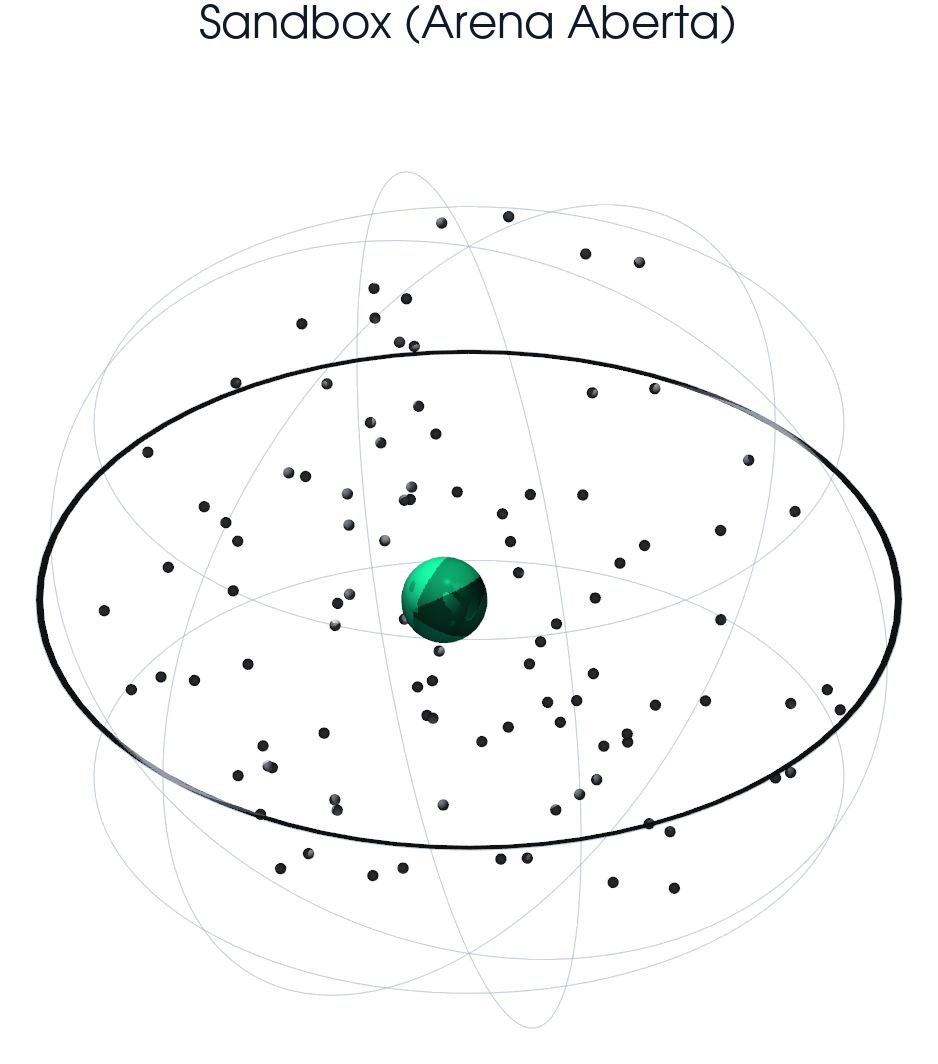
\includegraphics[width=0.29\textwidth]{images/mapa_3d_none.png}\hfill
    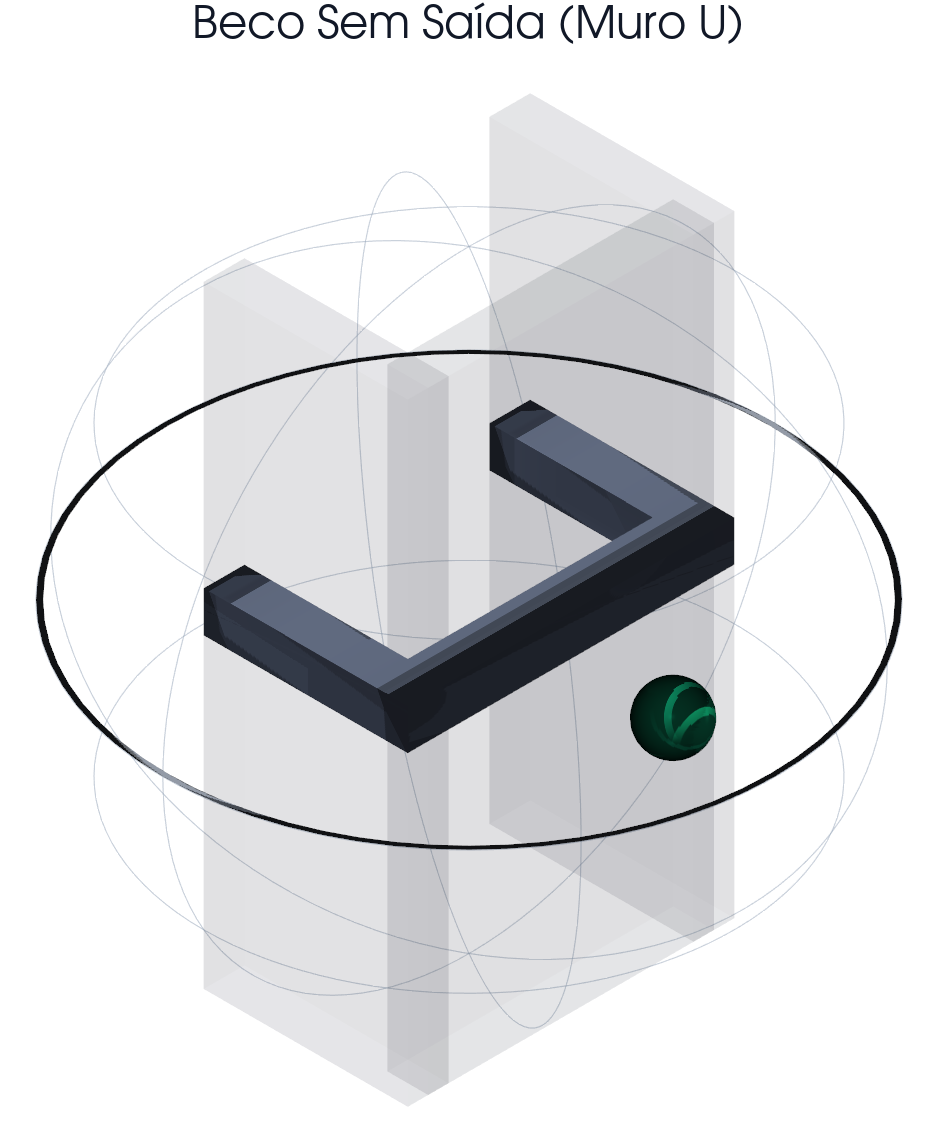
\includegraphics[width=0.29\textwidth]{images/mapa_3d_u_wall.png}\hfill
    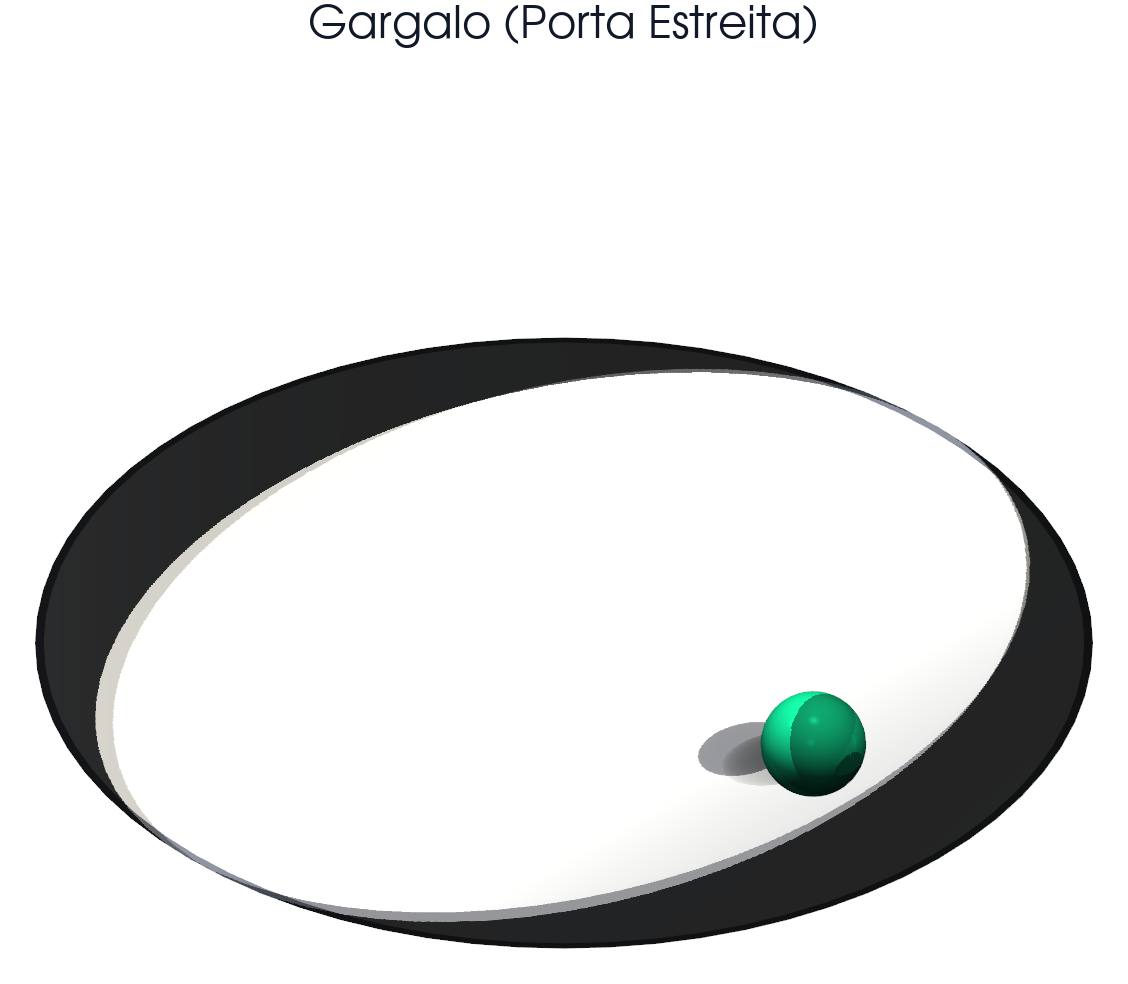
\includegraphics[width=0.29\textwidth]{images/mapa_3d_bottleneck.png}\\[0.4em]
    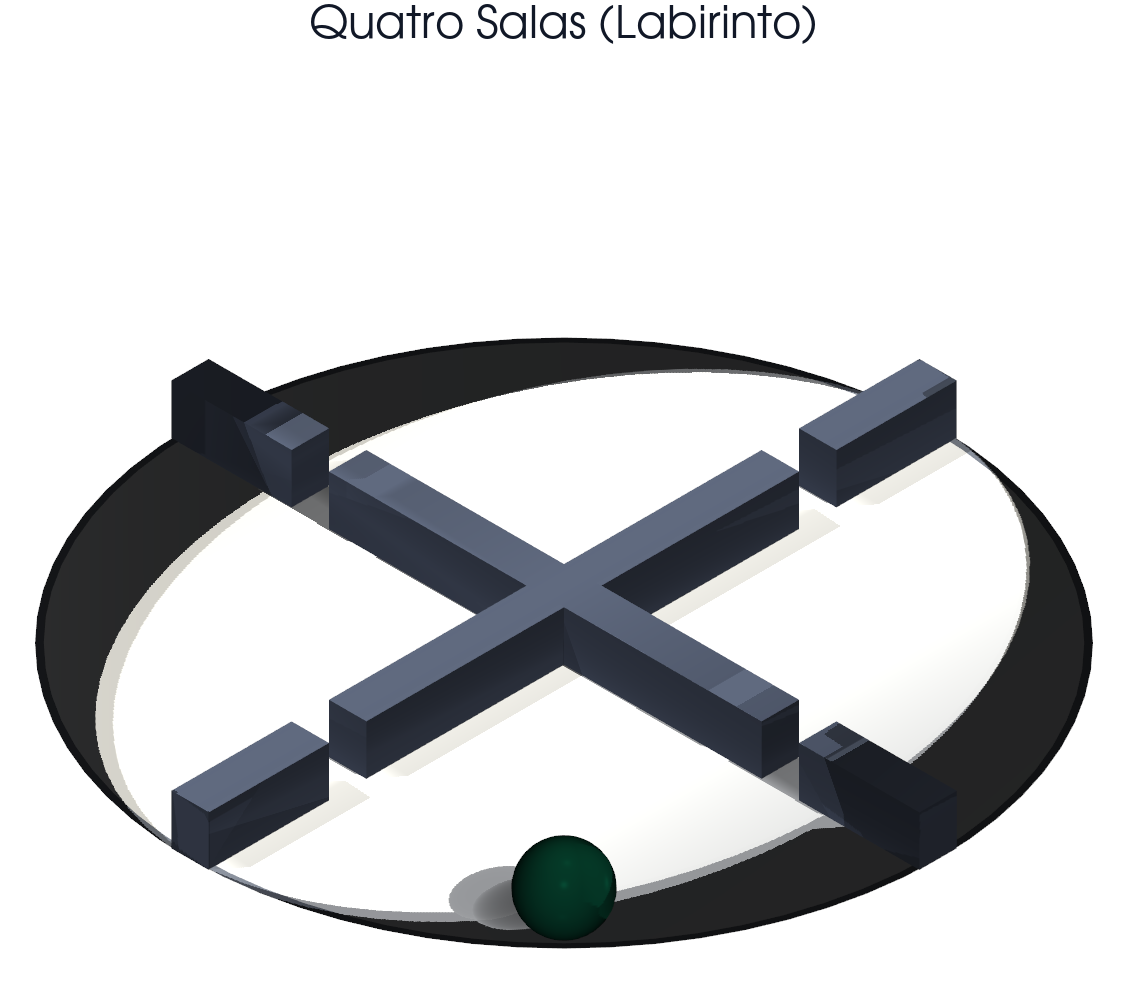
\includegraphics[width=0.29\textwidth]{images/mapa_3d_four_rooms.png}\hfill
    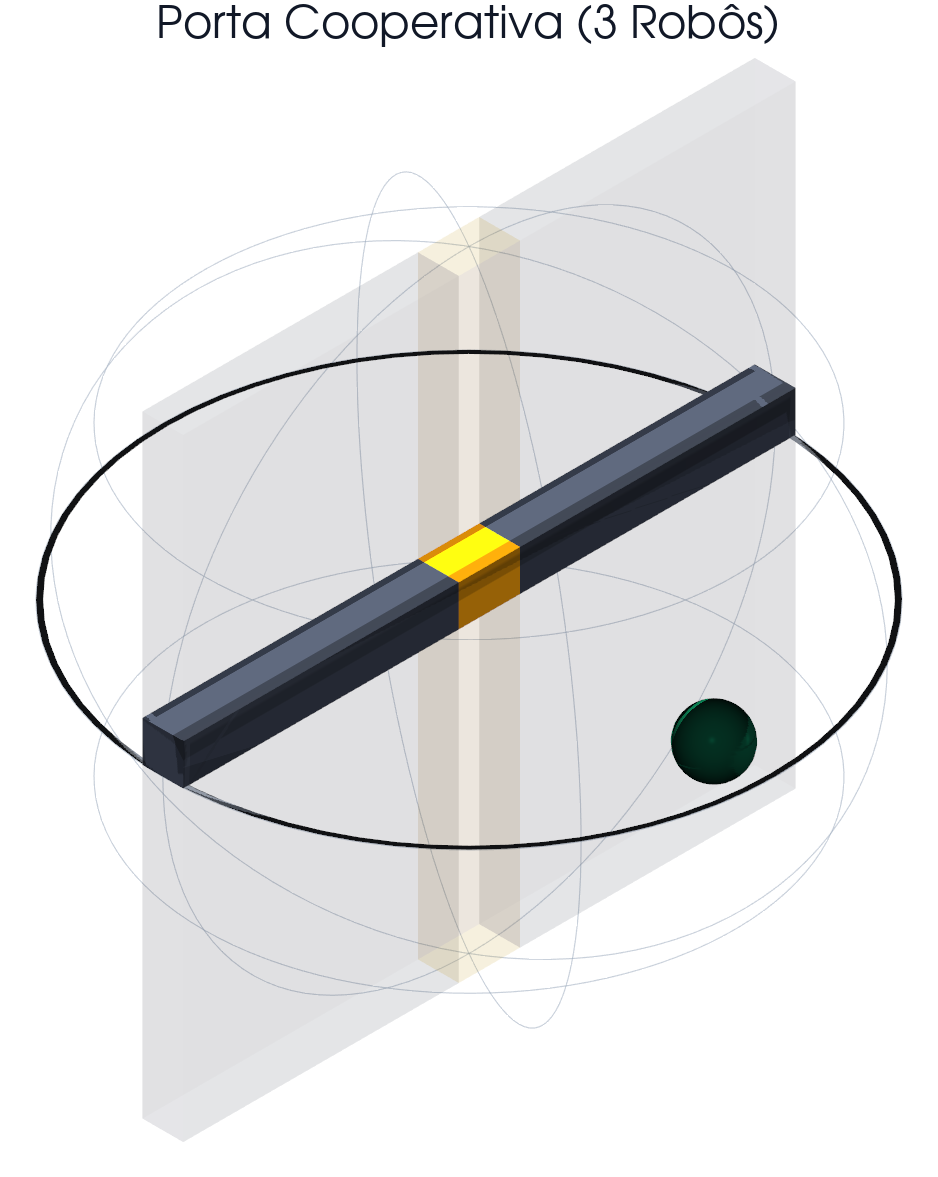
\includegraphics[width=0.29\textwidth]{images/mapa_3d_cooperative_door.png}\hfill
    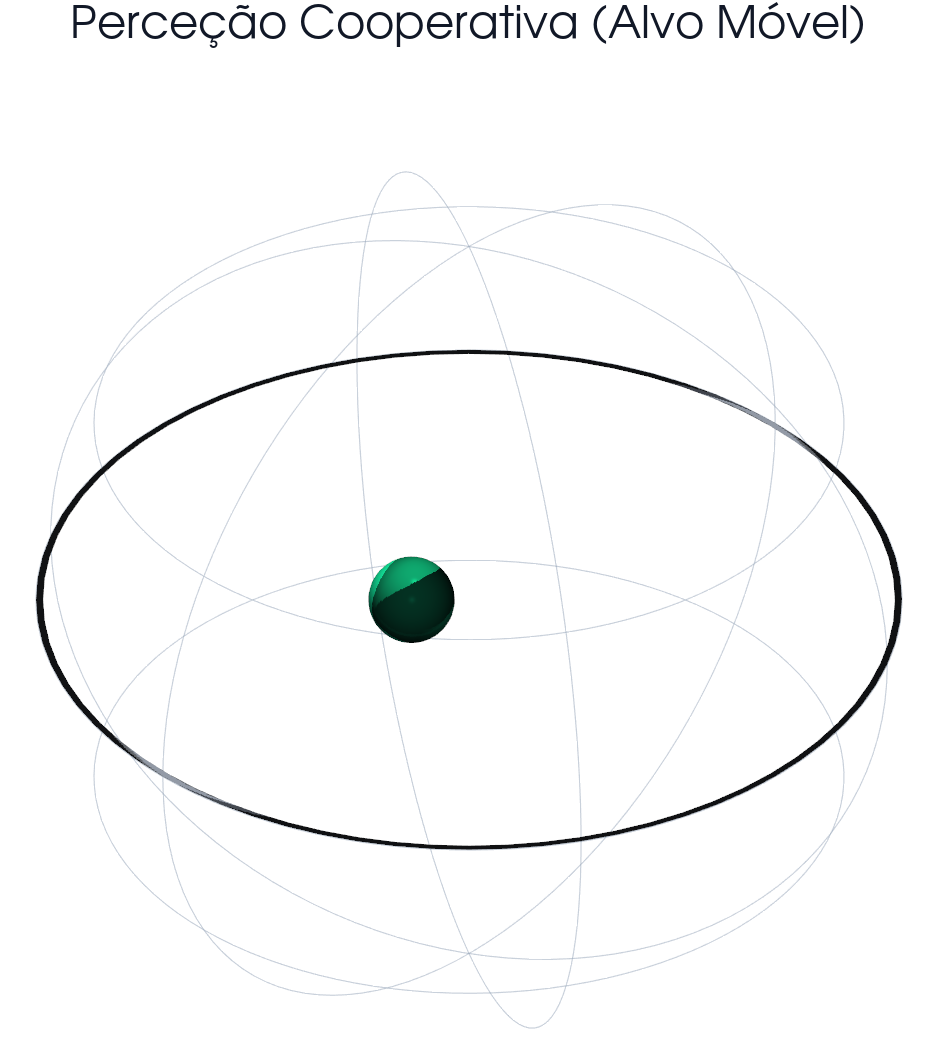
\includegraphics[width=0.29\textwidth]{images/mapa_3d_cooperative_perception.png}\\[0.4em]
    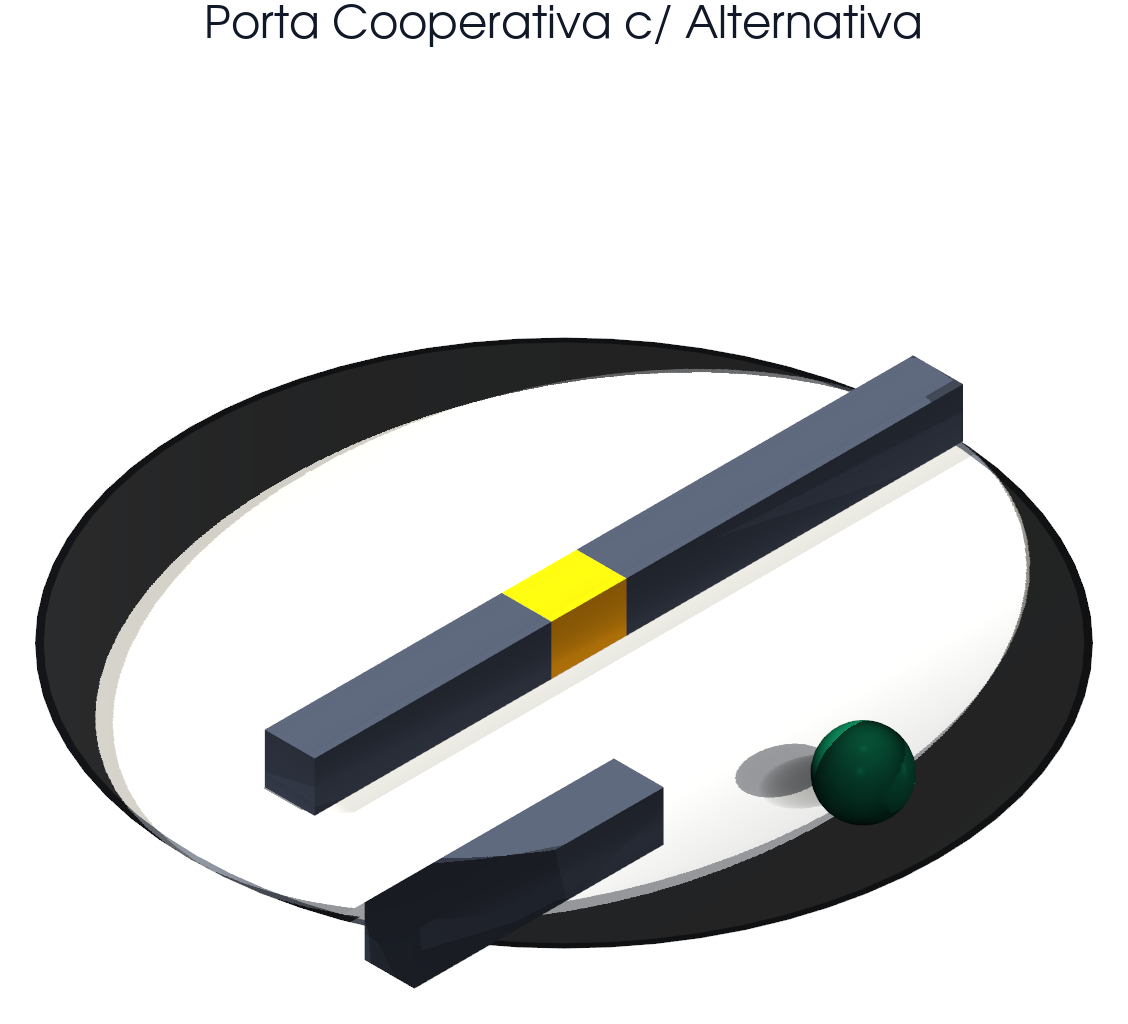
\includegraphics[width=0.29\textwidth]{images/mapa_3d_cooperative_door_bypass.png}
    \caption[Renderizações 3D dos sete cenários de teste]{Renderizações 3D dos sete cenários de teste, geradas a partir da geometria real do simulador (\texttt{scripts/render\_maps.py}). Em cima, da esquerda para a direita: Sandbox, Beco Sem Saída (Muro em U) e Gargalo; ao centro: Quatro Salas, Porta Cooperativa (com a porta destacada a âmbar) e Perceção Cooperativa; em baixo: Porta Cooperativa com Alternativa (\textit{bypass}). A esfera verde assinala o ninho (ou o alvo móvel, na Perceção Cooperativa) e as esferas cinzentas os obstáculos. A malha de círculos é a fronteira do domínio, que é uma \emph{esfera} de raio $15$\,m; o anel escuro marca a circunferência de referência $z=0$. Cada parede aparece duas vezes: sólida, com altura ilustrativa de $2$\,m, e em cinzento translúcido com o volume real. A leitura da figura está detalhada no texto desta secção.}
    \label{fig:cenarios_3d}
\end{figure}

\begin{figure}[!htbp]
    \centering
    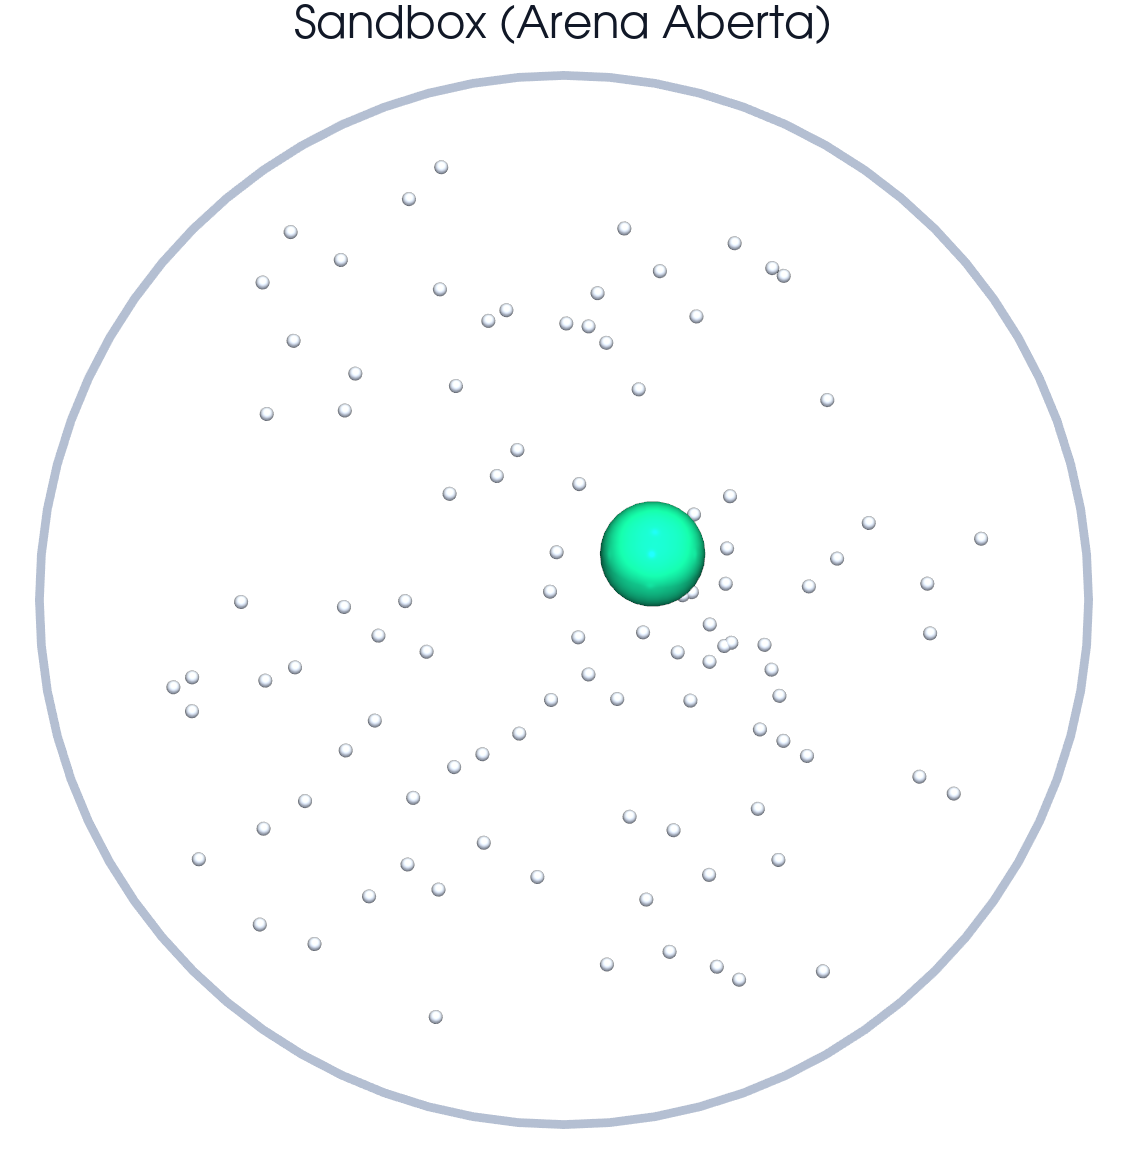
\includegraphics[width=0.30\textwidth]{images/mapa_topo_none.png}\hfill
    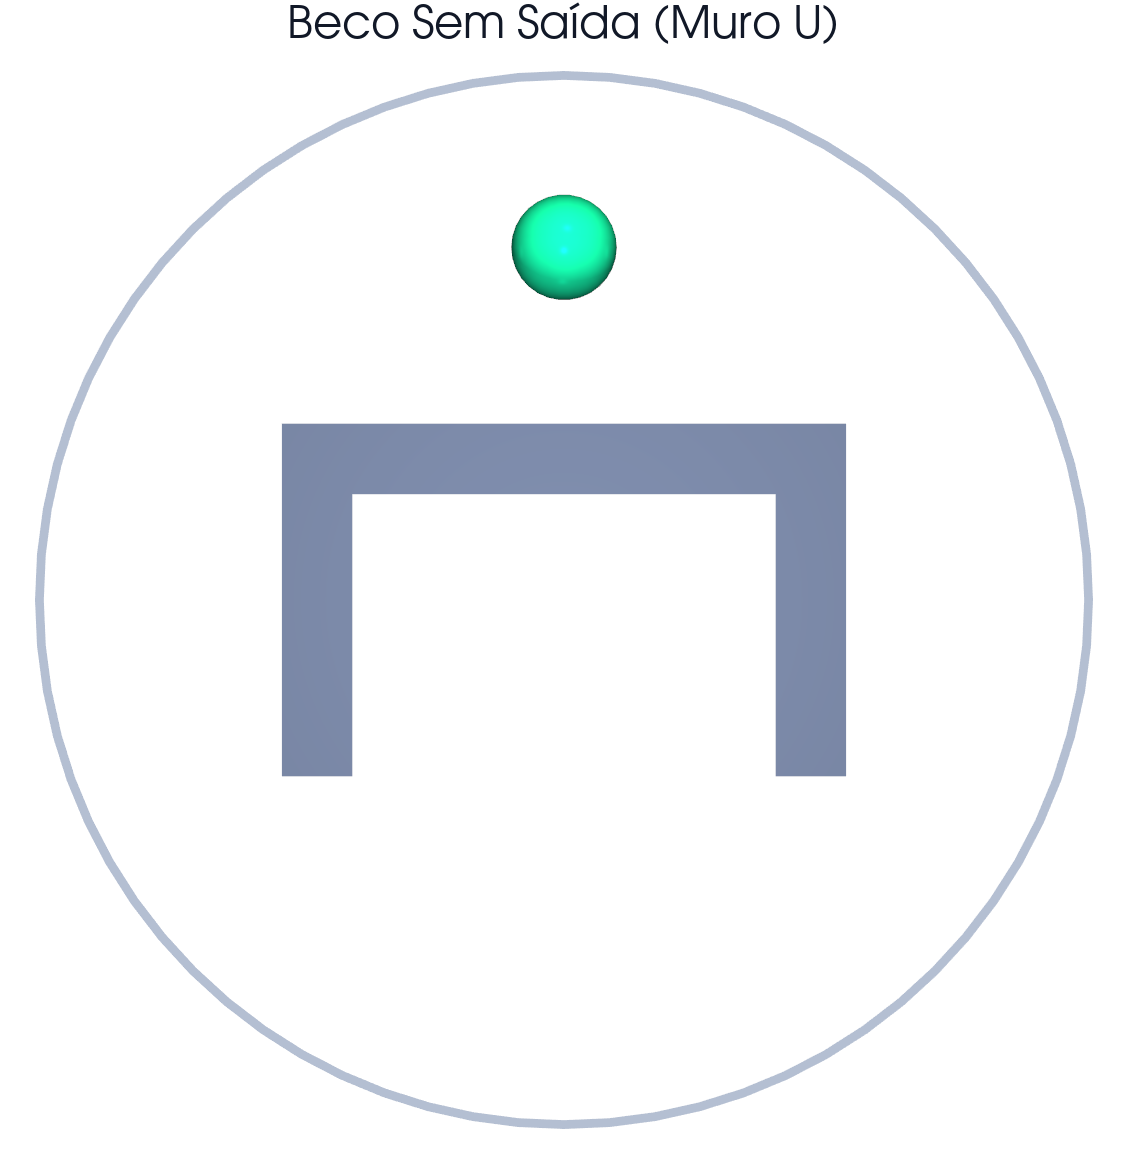
\includegraphics[width=0.30\textwidth]{images/mapa_topo_u_wall.png}\hfill
    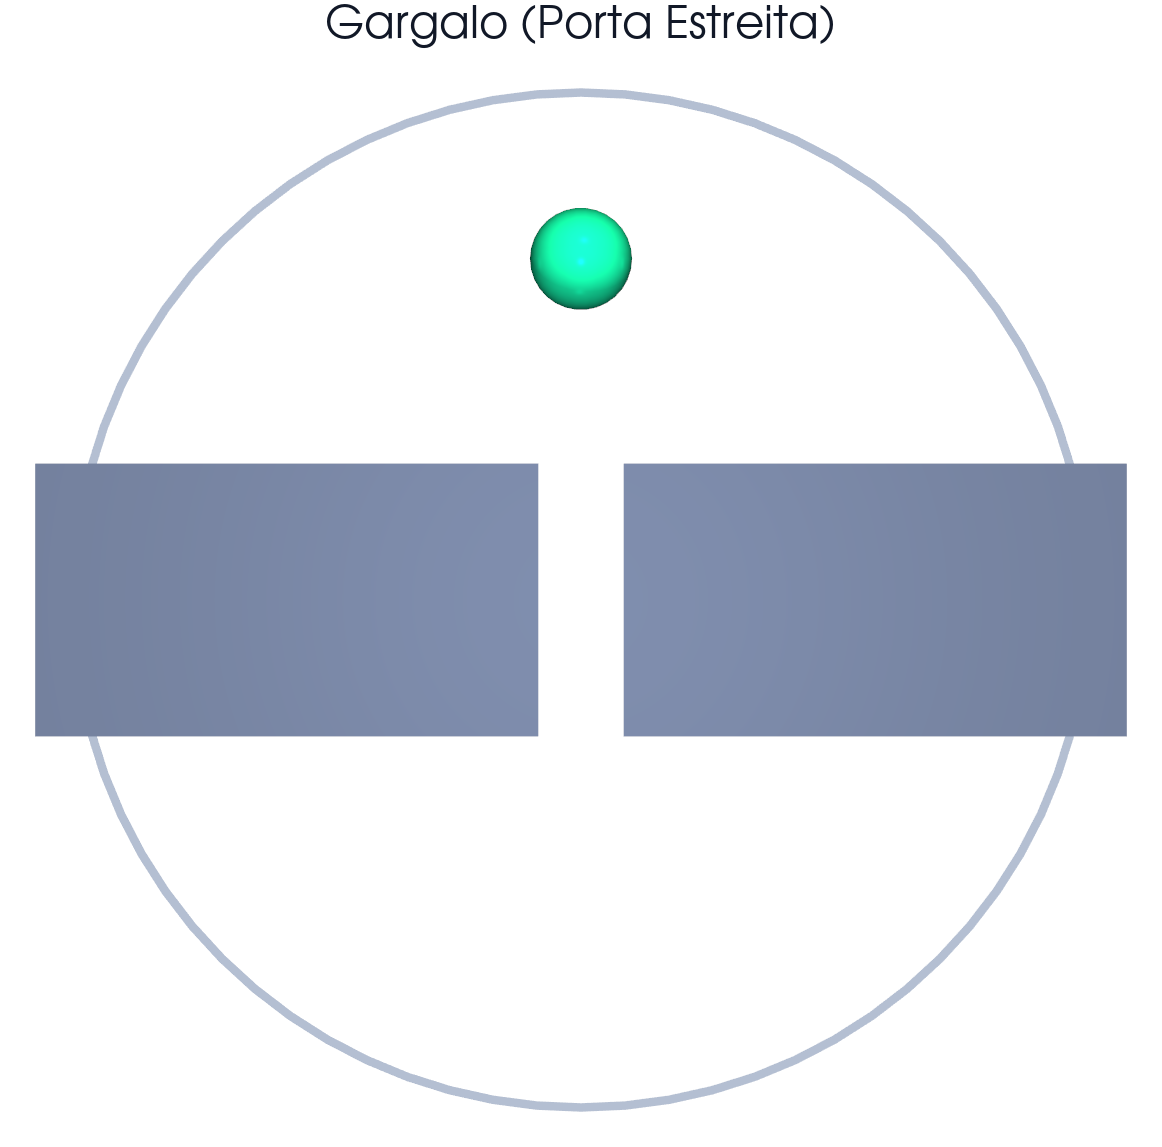
\includegraphics[width=0.30\textwidth]{images/mapa_topo_bottleneck.png}\\[0.4em]
    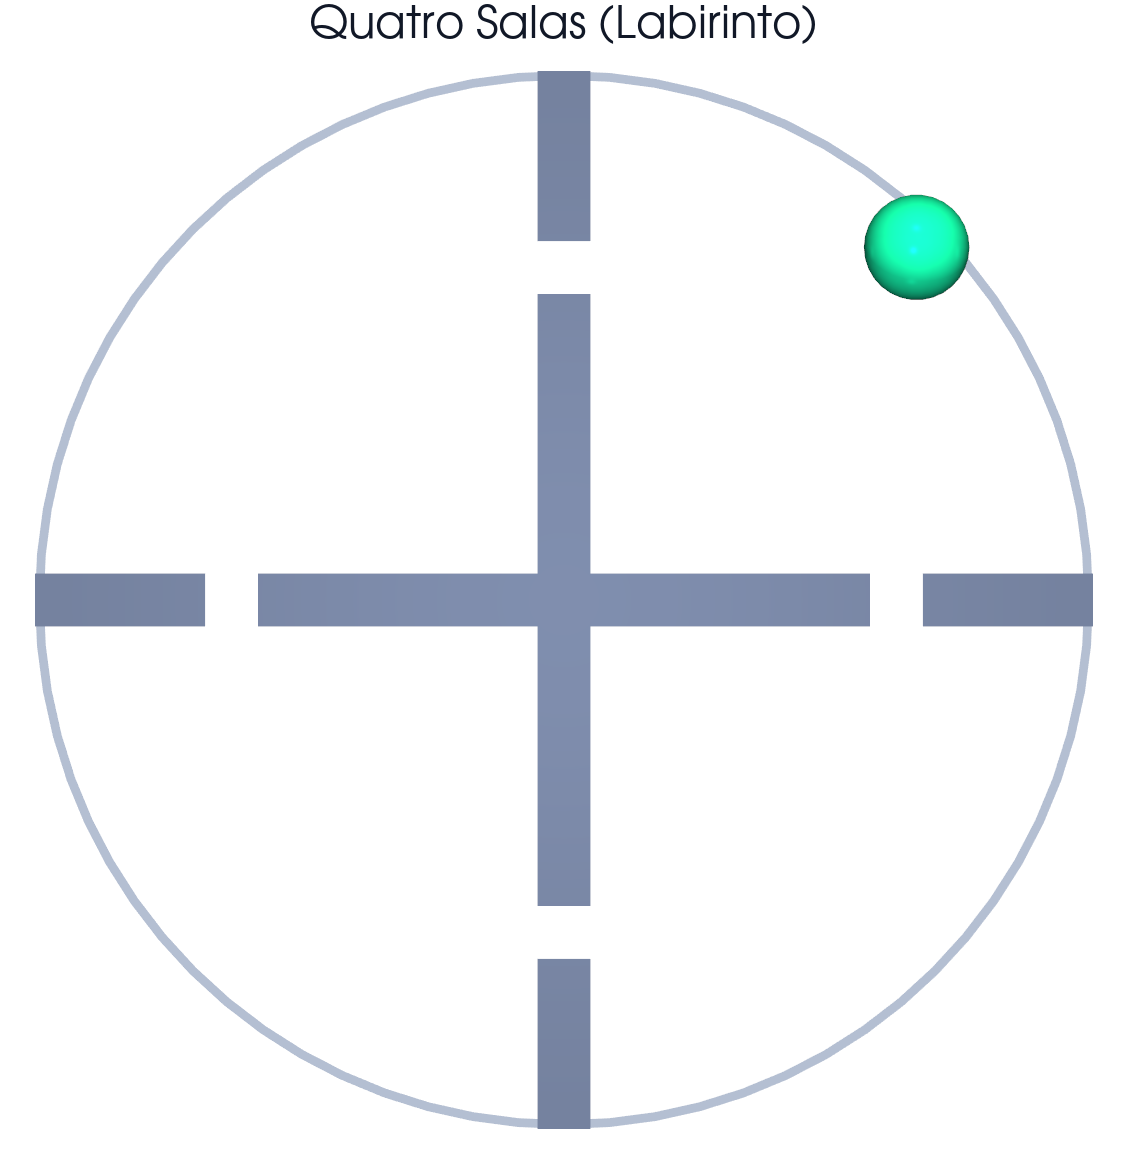
\includegraphics[width=0.30\textwidth]{images/mapa_topo_four_rooms.png}\hfill
    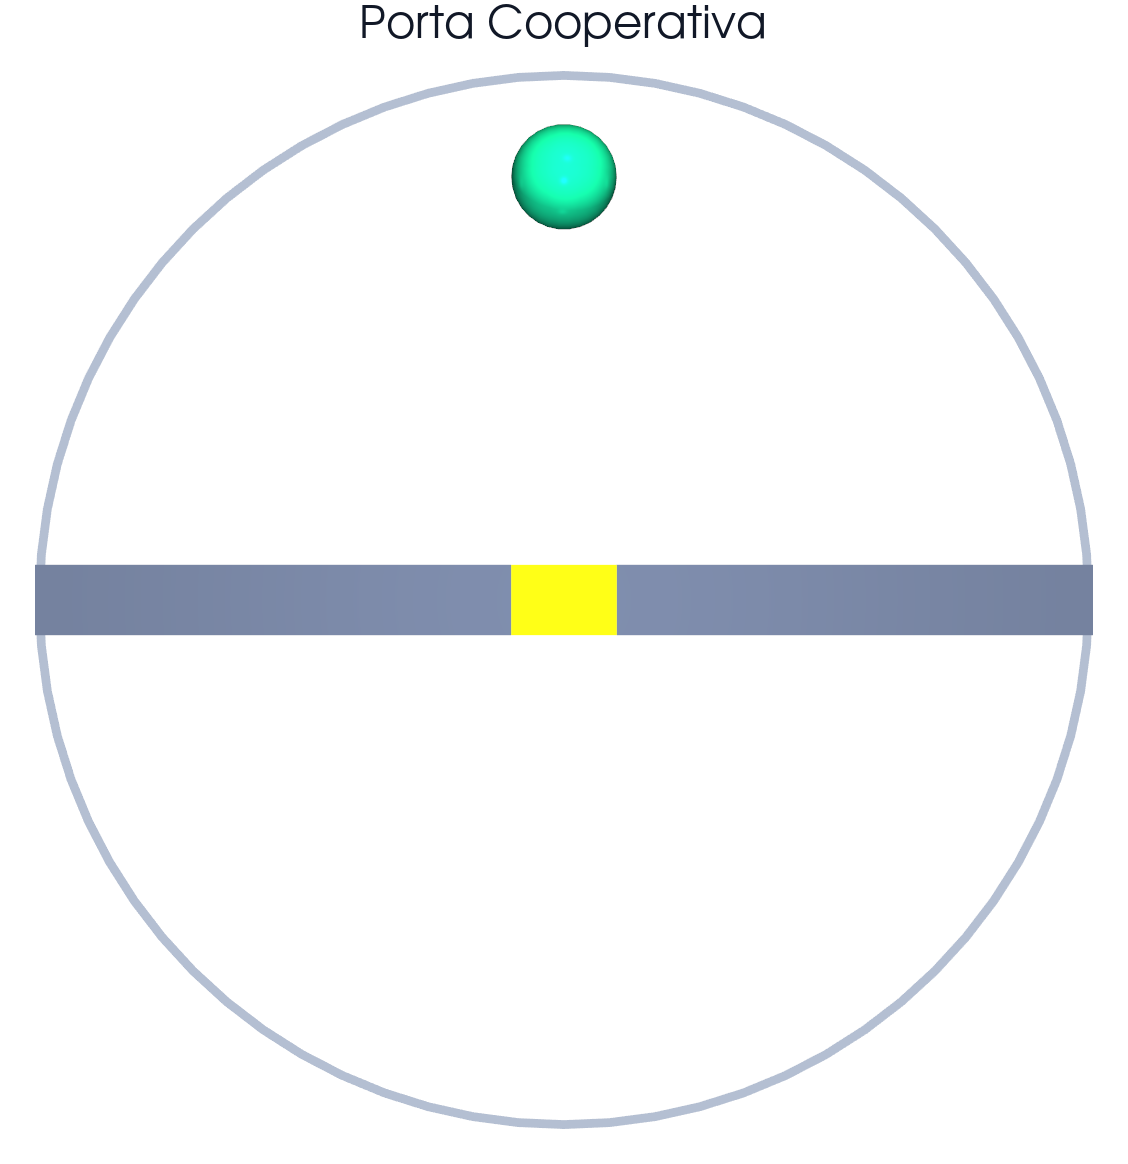
\includegraphics[width=0.30\textwidth]{images/mapa_topo_cooperative_door.png}\hfill
    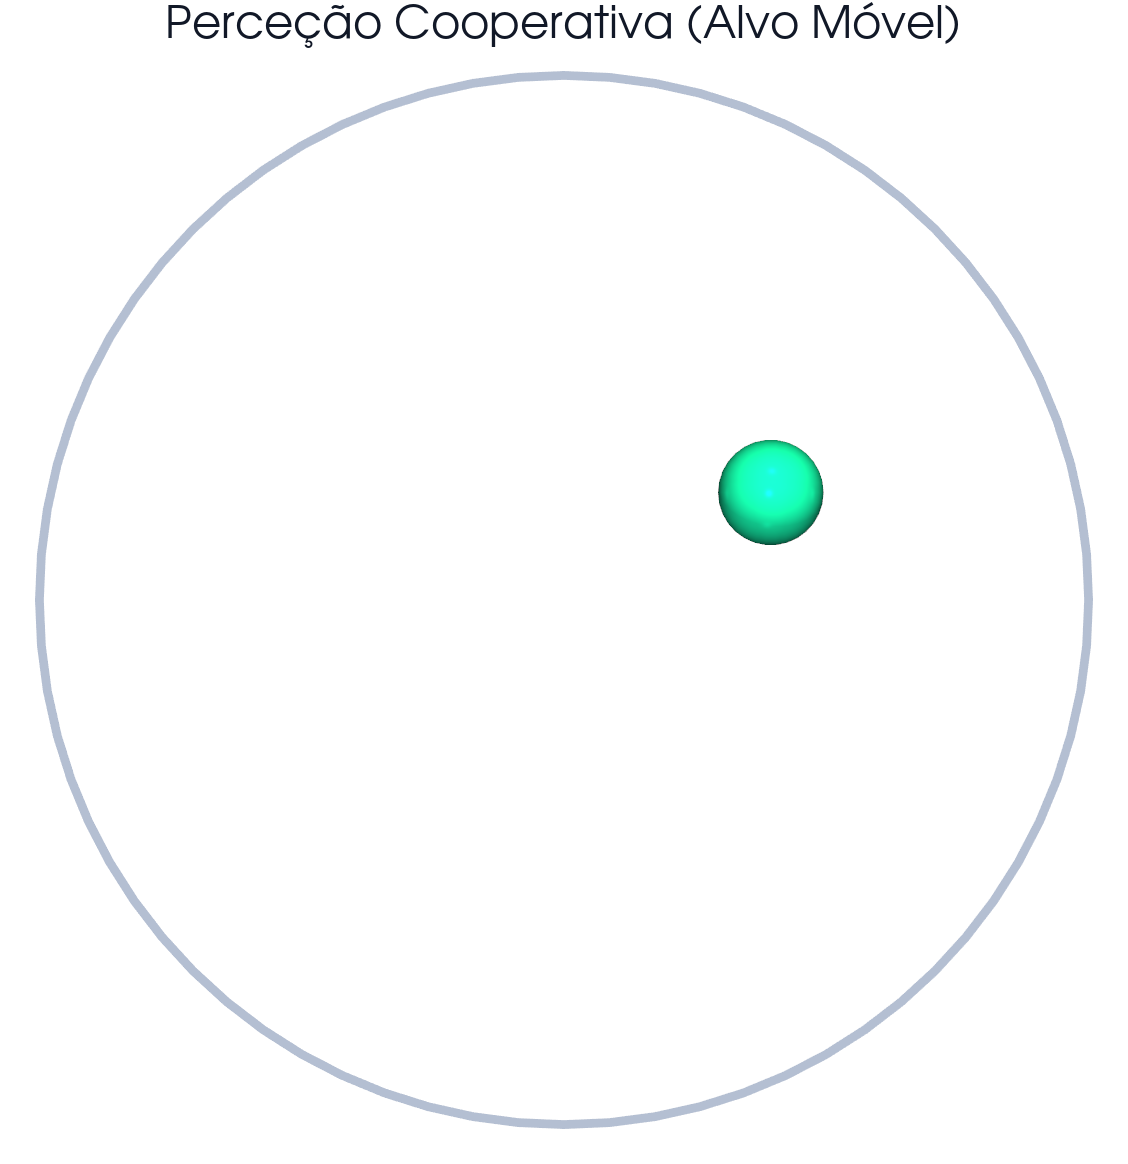
\includegraphics[width=0.30\textwidth]{images/mapa_topo_cooperative_perception.png}\\[0.4em]
    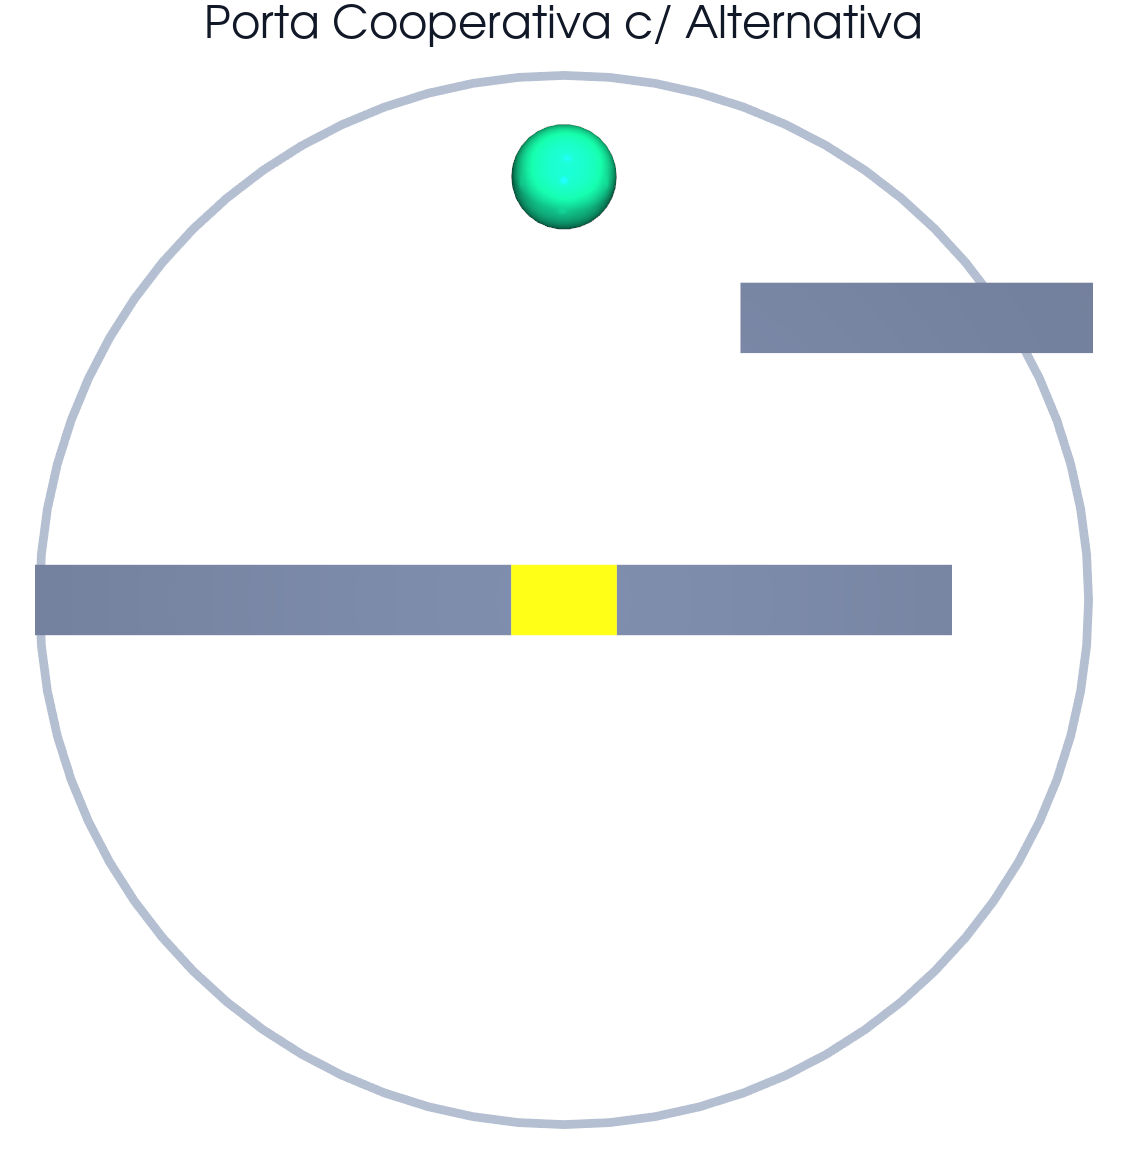
\includegraphics[width=0.30\textwidth]{images/mapa_topo_cooperative_door_bypass.png}
    \caption[Vista de topo (planta) dos sete cenários]{Vista de topo (planta) dos sete cenários, evidenciando a geometria das paredes e a posição relativa do ninho. As dimensões (comprimentos das paredes e largura das passagens) estão no texto desta secção; as plantas são esquemáticas e não têm escala impressa. Mesma ordem da Figura~\ref{fig:cenarios_3d}: em cima, Sandbox, Muro em U e Gargalo; ao centro, Quatro Salas, Porta Cooperativa e Perceção Cooperativa; em baixo, Porta Cooperativa com Alternativa.}
    \label{fig:cenarios_topo}
\end{figure}

\begin{enumerate}
    \item \textbf{Arena Aberta (Sandbox):} Cenário base sem barreiras fixas. Contém os agentes, obstáculos dinâmicos e um ninho móvel. Serve para aferir a cooperação no ninho sem a dificuldade adicional de navegar entre paredes.
    
    \item \textbf{Beco Sem Saída (Muro em U):} Um grande obstáculo em forma de ``U'' bloqueia a linha direta ao ninho. A parede superior tem $14$\,m e as pernas laterais têm $10$\,m. Os agentes começam do lado de fora da ``taça'' e têm de explorar lateralmente as aberturas de $7$\,m. Avalia a exploração prolongada em detrimento da navegação gananciosa.

    \item \textbf{Gargalo (Porta Estreita):} A arena é cortada a meio por uma parede contínua, deixando apenas uma passagem de $2{,}5$\,m de largura. Obriga o enxame a alinhar-se e a gerir o fluxo, e penaliza o congestionamento na passagem.

    \item \textbf{Quatro Salas (Labirinto):} Duas grandes paredes cruzam a arena vertical e horizontalmente, criando quatro salas isoladas ligadas apenas por aberturas de $2{,}5$\,m de largura. Os agentes começam no extremo oposto ao ninho, exigindo navegação estruturada de longo alcance, sem que nenhum dos controladores disponha de memória.

    \item \textbf{Porta Cooperativa:} Similar ao Gargalo, mas a passagem de $3$\,m de largura encontra-se bloqueada por um portão físico. A porta só abre (deslizando para fora do caminho, com realce visual no \textit{dashboard}) quando no mínimo 3 agentes ocupam a zona de pressão em simultâneo. Por exigir uma sincronização mais demorada, este cenário dispõe de um horizonte temporal alargado de $800$ passos (face aos $500$ dos restantes), dando margem para que o enxame coordene a abertura e ainda alcance o ninho. Foca-se em comportamentos de sincronização sem comunicação explícita.

    \item \textbf{Perceção Cooperativa (Alvo Móvel):} A noção de ``ninho físico'' desaparece. O alvo de interesse viaja livremente pelo mapa ao dobro da velocidade normal ($0{,}03$\,m/s). Só é considerado capturado quando $3$ agentes se aproximam a menos de $4$\,m de distância e se distribuem num raio de 360\textdegree{} em redor do mesmo, testando manobras de cerco e perseguição.

    \item \textbf{Porta Cooperativa com Alternativa (\textit{Bypass}):} Variante da Porta Cooperativa desenhada como problema de \emph{recompensa enganadora} (\textit{deceptive}). A barreira horizontal mantém a porta central de $3$\,m (que continua a exigir 3 agentes na zona de pressão), mas o segmento direito da barreira termina antes da fronteira da arena, deixando uma abertura permanentemente livre de $4$\,m junto à parede leste --- um percurso alternativo que dispensa cooperação. Uma parede defletora, colocada mais a norte no mesmo lado, obriga quem usa a alternativa a afastar-se temporariamente do ninho, tornando o percurso alternativo cerca de duas vezes mais longo do que a passagem pela porta. A rota mais curta atrai, assim, o enxame para a porta (que exige coordenação), enquanto a descoberta da alternativa exige contrariar o gradiente de aproximação ao objetivo --- a propriedade que faz deste o cenário de referência para a QI6 (procura por novidade, Secção~\ref{sec:questoes_investigacao}). Pelo horizonte de exploração acrescido, o limite temporal é alargado para $1000$ passos.
\end{enumerate}

\section{Design da Função de Recompensa}
\label{sec:reward_design}
A função de recompensa é o instrumento de desenho experimental mais sensível do sistema: as primeiras campanhas de treino acumularam termos secundários (penalizações de dispersão, de colisão entre agentes e de contacto com obstáculos) que, na prática, diluíam o sinal da tarefa e abriam portas a comportamentos degenerados. A formulação final adotou deliberadamente uma \emph{recompensa simples}, com o número mínimo de termos e dois focos --- \emph{explorar o mapa} e \emph{encontrar o ninho} --- em que a recompensa de tarefa domina claramente todos os sinais de \textit{shaping}. As penalizações secundárias foram removidas \emph{apenas do sinal de treino}: a resolução física correspondente mantém-se no motor (os agentes continuam a não se sobrepor nem a atravessar paredes, Secção~\ref{sec:eng_fisica}), pelo que a simplificação não altera a dinâmica do mundo, apenas o que é ensinado.

\begin{equation}
    \mathcal{R}(s, \mathbf{a}) = R_{\text{tarefa}} + R_{\text{progresso}} + R_{\text{exploração}} - R_{\text{controlo}}
\end{equation}

Os valores exatos utilizados na campanha experimental final são os seguintes:
\begin{itemize}
    \item \textbf{Tarefa ($R_{\text{tarefa}}$):} Recompensa dominante de $+300$ por chegada, atribuída (e \emph{repetível} ao longo do episódio) a cada agente que participa numa chegada bem sucedida. O número de agentes exigidos em simultâneo no ninho ($k_{min}$) é definido \emph{por cenário}: $k_{min}=3$ nos cenários em que a cooperação é o objeto de estudo (Sandbox, Porta Cooperativa, Perceção Cooperativa e \textit{Bypass}), mas $k_{min}=1$ nos labirintos de navegação pura (Muro em U, Gargalo e Quatro Salas) --- exigir três agentes simultâneos nesses cenários transformava um problema de navegação numa cooperação artificial, registando zero chegadas mesmo quando um ou dois agentes alcançavam o ninho. Nos cenários com porta cooperativa acresce um bónus único de $+100$ a cada agente que participa na abertura da porta.
    \item \textbf{Progresso ($R_{\text{progresso}}$):} Baseado no método \textit{Potential-Based Reward Shaping} (PBRS) \cite{ng1999policy}, atribui $10{,}0 \cdot (\Phi_{t-1} - \Phi_{t})$, onde $\Phi$ é o \emph{potencial de navegação} até ao ninho. Nos cenários com paredes (Muro em U, Gargalo, Quatro Salas e as duas Portas Cooperativas) este potencial é a \emph{distância geodésica} --- o comprimento do caminho mais curto que contorna os obstáculos, calculado por uma pesquisa de custo uniforme (Dijkstra, 8-conexa) sobre uma grelha de discretização ($0{,}4$\,m, com as paredes dilatadas pelo raio do robô) --- e não a distância euclidiana. Esta escolha elimina na raiz um mínimo local clássico: com a distância euclidiana, contornar uma parede \textit{afasta} o agente do ninho e é penalizado, prendendo o enxame contra os obstáculos; com a distância geodésica, qualquer passo ao longo do caminho viável é recompensado. Em rigor, a garantia de invariância de Ng et al.\ exige o termo $\gamma\Phi_{t}$ em vez de $\Phi_{t}$; como aqui o fator $\gamma=0{,}99$ é omitido, o termo difere do PBRS por uma penalização $10{,}0\,(1-\gamma)\,\Phi_{t}$, proporcional à distância ao ninho e alinhada com a tarefa, pelo que a política ótima se preserva apenas de forma aproximada \cite{ng1999policy}. Decisivamente, o campo geodésico é um \emph{sinal de treino} (a geometria é conhecida pelo simulador apenas durante o treino) e \emph{não} uma observação: em execução o agente dispõe somente da bússola de \textit{homing} euclidiana e do LiDAR local (Secção~\ref{sec:obs_space}), preservando a observabilidade parcial. Distingue-se assim, claramente, de fornecer ao agente um mapa dos obstáculos ou \textit{waypoints} de um planeador A*.
    \item \textbf{Exploração ($R_{\text{exploração}}$):} Bónus de exploração \textit{count-based} que atribui $+0{,}5$ na primeira vez que um agente visita cada célula de uma grelha de discretização espacial ($2 \times 2$\,m), em linha com a necessidade de mecanismos densos de exploração identificada por Xiao et al. (2026) \cite{xiao2026csper}. O valor é \emph{pequeno de propósito}: incentiva a cobertura do mapa em regiões onde o gradiente do potencial é pouco informativo, mas é dominado por larga margem pela recompensa de tarefa ($+300$, repetível). Iterações anteriores com um bónus maior demonstraram o risco desta calibração: a política aprendia a \emph{vaguear} para colher exploração em vez de convergir para a chegada --- um caso de \textit{reward hacking} que motivou a simplificação da recompensa aqui descrita, e cujo análogo evolutivo (\textit{fitness exploitation}) se analisa na Secção~\ref{sec:res_discussao}.
    \item \textbf{Controlo Energético ($R_{\text{controlo}}$):} Subtração de $0{,}05$ a cada passo de simulação por agente não inativo. Pressiona temporalmente o enxame para chegar ao ninho o mais depressa possível; nos cenários de objetivo fixo é a única fonte de pressão temporal.
    \item \textbf{Fome (cenários sem campo geodésico):} Caso o temporizador de \textit{hunger} de um agente ultrapasse 250 passos, o agente ``morre'', sofre um revés de $-50{,}0$ e a sua posição é restabelecida no ponto de partida. Esta reposição está \emph{ativa apenas nos cenários sem campo geodésico} (Sandbox e Perceção Cooperativa); nos labirintos, em que o potencial de progresso é geodésico, foi desativada, pois a combinação do teletransporte com a re-sincronização do potencial tornava o termo de progresso \textit{farmável} (aproximar-se, ser reposto longe sem cobrança do recuo, repetir), induzindo políticas degeneradas que acumulavam recompensa de \textit{shaping} sem nunca cumprir a tarefa.
    \item \textbf{Penalizações secundárias (desativadas na formulação final):} As versões preliminares incluíam penalizações de \textit{anti-clustering} (proximidade entre agentes), de colisão agente--agente e de contacto com obstáculos. Na formulação final, os respetivos pesos foram colocados a zero: a separação física e o \textit{push-out} continuam a ser \emph{resolvidos} pelo motor (Secção~\ref{sec:eng_fisica}), mas deixaram de gerar sinal de recompensa, eliminando três termos cuja calibração relativa baralhava o sinal da tarefa. Definiu-se como salvaguarda experimental que, caso surgissem comportamentos degenerados (agregação excessiva ou agentes ``colados'' às paredes), os termos seriam reintroduzidos gradualmente --- o que não se revelou necessário.
\end{itemize}

\section{Desafios de Engenharia e Otimização Computacional}
O treino por reforço exige milhões de passos de simulação, pelo que o custo de cada passo decide o que é possível treinar. Esta secção descreve as opções de engenharia do ambiente (\texttt{swarm\_env\_3d.py}) e dos visualizadores 3D que mantêm esse custo baixo.

\subsection{Motor de Visualização Interativa (Dashboard)}
Para se poder inspecionar o comportamento do enxame sem abrandar o treino, a simulação está separada da renderização gráfica.
A inspeção do comportamento é feita por um visualizador 3D implementado com o motor \emph{Ursina} (assente em Panda3D), que projeta a telemetria do motor contínuo interno num espaço tridimensional navegável, com representação do ninho, obstáculos móveis, muros e indicadores de proximidade. O controlo experimental --- lançamento de treinos, seleção de cenários e geração de gráficos --- é centralizado num \textit{dashboard} interativo construído em \emph{NiceGUI} (aplicação \textit{web} local). Esta separação permite que o simulador opere num modo \textit{headless} (sem sobrecarga gráfica) durante sessões de treino intensivo --- processando milhares de transições por segundo ---, enquanto oferece um modo interativo para demonstração e análise qualitativa das políticas aprendidas.

\subsection{Otimização Matemática da Física e Deteção de Colisões}
\label{sec:eng_fisica}
Cada passo de simulação tem de levar poucos milissegundos. Com $N=20$ agentes e uma centena de obstáculos móveis, o custo da deteção de colisões cresce com o número de pares a testar, pelo que as operações são vetorizadas.
\begin{itemize}
    \item \textbf{Deteção Geométrica de Colisões:} O motor resolve as colisões por testes geométricos diretos --- distância Euclidiana para os obstáculos esféricos e caixas envolventes alinhadas aos eixos (\textit{Axis-Aligned Bounding Boxes}, AABB) para os muros retangulares ---, recorrendo a operações vetoriais \emph{NumPy} no cálculo de distâncias e profundidades de penetração. Um passo dedicado de \emph{separação física} repele geometricamente qualquer par de agentes sobrepostos, assegurando a ausência de interpenetrações não-físicas no enxame.
    \item \textbf{Wall-Sliding Cinemático:} Quando um robô entra em contacto com uma parede retangular, o motor não o imobiliza mecanicamente (o que penalizaria irreversivelmente a exploração do algoritmo MARL). Em vez disso, remove a componente do deslocamento segundo a normal da superfície de colisão, e o agente desliza ao longo da parede (\textit{wall-sliding}). É uma simplificação cinemática: um chassis \textit{differential-drive} real não desliza lateralmente desta forma.
\end{itemize}

\subsection{Mecanismo de Atenção sobre Vizinhos (GNN)}
O extrator de relações entre robôs foi implementado de raiz em \emph{PyTorch puro} (sem recurso a bibliotecas de grafos como o PyTorch Geometric), através de um mecanismo de \emph{atenção de produto interno escalado} sobre o conjunto de vizinhos, conforme formalizado nas Equações~\ref{eq:qkv}--\ref{eq:msg_pool}.
\begin{itemize}
    \item \textbf{Representação Densa da Vizinhança:} A cada passo, cada agente $i$ observa os restantes $N-1$ agentes através de um vetor de \textit{features} de dimensão fixa (direção egocêntrica, distância normalizada e sinal de comunicação por vizinho). Diferentemente de uma abordagem baseada em arestas esparsas com raio de comunicação fixo, todos os vizinhos são apresentados ao módulo de atenção, sendo a \emph{relevância de cada um aprendida} pelos coeficientes $\alpha_{ij}$ --- a rede atribui dinamicamente pesos próximos de zero aos vizinhos irrelevantes, dispensando um corte geométrico explícito.
    \item \textbf{Dimensão Fixa e \textit{Parameter Sharing}:} Com $N=20$, a observação tem dimensão fixa ($\mathbb{R}^{111}$), pelo que a integração em \textit{batches} de treino é direta, sem necessidade de \textit{padding} dinâmico ou conversão para listas de índices. Já as projeções \textit{Query}-\textit{Key}-\textit{Value} e o \textit{softmax} operam sobre o número de vizinhos presentes, pelo que a mesma rede processa enxames de qualquer dimensão --- viabilizando o \textit{Zero-Shot Transfer} para $N \in \{10, 50, 100\}$ sem retreino.
\end{itemize}

\subsection{Ambientes Vetorizados e Paralelização Multiprocesso}
A recolha de experiência (PPO e SAC) e a avaliação da população evolutiva correm em paralelo:
\begin{itemize}
    \item \textbf{Vectorized Environments:} O ambiente é envolvido pelo \textit{wrapper} \texttt{SubprocVecEnv} da \textit{Stable-Baselines3}, que corre 16 cópias do simulador em processos de CPU separados.
    \item \textbf{Mecanismo de Guilhotina (Early Stopping):} No treino evolutivo, um episódio cuja recompensa acumulada ao fim de 150 passos fique abaixo de um limiar é interrompido, e o genoma é penalizado (Secção~\ref{sec:evo_ciclo}). Evita-se assim gastar tempo de CPU a avaliar até ao fim genomas que a mutação tornou claramente disfuncionais.
\end{itemize}

\section{Estrutura do Projeto e Extensibilidade}
\label{sec:extensibilidade}
Um dos objetivos declarados desta dissertação é entregar uma \emph{implementação de referência} reutilizável (Secção~\ref{sec:contributos}). Essa ambição obriga a tratar a estrutura do software como resultado, e não como detalhe de implementação: importa dizer, com precisão, o que custa a um terceiro estender este trabalho --- e o que \emph{não} foi desenhado para ser barato.

\subsection{Organização dos Módulos}
O repositório separa quatro responsabilidades, com dependências num só sentido (a simulação não conhece o treino, o treino não conhece a análise):

\begin{itemize}
    \item \texttt{src/} ($\approx$2\,300 linhas) --- o núcleo. Contém o ambiente (\path{environment/swarm_env_3d.py}: física, LiDAR, geodésicas, recompensa), os controladores (\texttt{agents/}: a rede \texttt{GNNAgent3D} e uma interface \texttt{Agent.get\_action}, hoje só usada pelo controlador aleatório de referência), os treinadores (\texttt{training/}: um módulo por paradigma) e o \emph{registo canónico de cenários} (\texttt{scenarios.py}).
    \item \texttt{scripts/} ($\approx$4\,100 linhas) --- a orquestração e a análise: \texttt{run\_experiments.py} (campanhas), a bateria de avaliação (\texttt{eval\_*.py}), os testes estatísticos e a geração de figuras.
    \item \texttt{dashboard/} ($\approx$2\,600 linhas) --- observabilidade: acompanhamento do treino, curvas ao vivo, matriz de resultados e ligação ao servidor remoto.
    \item \texttt{tests/} ($\approx$800 linhas) --- garantias de não-regressão, discutidas adiante.
\end{itemize}

\subsection{Pontos de Extensão}
\paragraph{Acrescentar um algoritmo é barato.} Um novo controlador exige (i) uma classe que produza a ação a partir da observação (uma rede PyTorch, como a \texttt{GNNAgent3D}, ou uma política da \textit{Stable-Baselines3}), (ii) um módulo de treino em \texttt{src/training/} e (iii) \emph{uma entrada} no dicionário \texttt{ALGORITHMS} de \texttt{run\_experiments.py}. A partir daí, o algoritmo é automaticamente incluído nas campanhas, na avaliação determinística, nos testes de significância e nas figuras --- porque toda a cadeia a jusante itera sobre esse registo, e não sobre nomes escritos à mão. A comparação MADDPG ou QMIX que a Secção~\ref{sec:limitacoes_trabalho_futuro} propõe é, neste sentido, um exercício de dias e não de semanas.

\paragraph{Acrescentar uma métrica ou um teste é barato.} As métricas de avaliação são calculadas num único ponto (\path{scripts/eval_suite.py}) e propagam-se por escrita em \path{results/evaluation/eval_summary.csv}, do qual dependem, por leitura, a análise estatística, os gráficos e o painel. Uma métrica nova torna-se visível em toda a cadeia sem alterar nenhum consumidor.

\paragraph{Acrescentar um cenário é barato \emph{à superfície} e caro \emph{no fundo}.} Os \emph{metadados} de cenário --- lista canónica, rótulos longos e curtos, classificação como labirinto --- residem num único ficheiro (\texttt{src/scenarios.py}), do qual todos os consumidores importam. Esta centralização não é acidental: resultou da correção de um defeito real, em que o sétimo cenário foi treinado mas nunca avaliado, por a lista de cenários estar duplicada entre os módulos de treino e de avaliação. Com a fonte única, um cenário novo aparece automaticamente nas campanhas, nos quadros e nas figuras.

A \emph{geometria}, porém, não goza da mesma disciplina: a construção de paredes, as posições de \textit{spawn} e as regras específicas de cada cenário estão distribuídas por doze blocos condicionais (\texttt{if classic\_scenario == \dots}) dentro do ambiente. Acrescentar um cenário implica, portanto, tocar em vários pontos de um ficheiro extenso --- um custo que cresce linearmente com o número de cenários e que constitui a dívida técnica mais visível deste projeto. A correção natural é um \emph{registo de cenários} análogo ao dos algoritmos: cada cenário passaria a ser uma classe com uma interface fixa (\texttt{build\_obstacles}, \texttt{spawn\_positions}, \texttt{required\_to\_eat}), registada por decorador, e os doze condicionais colapsariam numa única invocação polimórfica. A refatoração é direta e está identificada; não foi executada porque as campanhas experimentais já tinham começado e qualquer alteração ao ambiente invalidaria a comparabilidade dos resultados já obtidos --- precisamente o tipo de compromisso entre pureza arquitetural e integridade experimental que uma dissertação empírica impõe.

\subsection{Garantias de Não-Regressão}
A extensibilidade só é real se o sistema puder ser alterado sem medo. Para esse efeito, as otimizações de desempenho mais arriscadas foram acompanhadas de \emph{testes de equivalência bit-a-bit} contra a implementação de referência: a vetorização do LiDAR (adotada por multiplicar o \textit{throughput} por $\approx 19$) é confrontada com o ciclo explícito original em $8\,000$ cenas aleatórias --- incluindo casos-limite como raios paralelos aos eixos e ausência de obstáculos ---, exigindo-se igualdade \emph{exata}; a vetorização das observações egocêntricas ($\approx 2{,}6\times$ no passo de simulação) é verificada do mesmo modo. A mecânica da porta cooperativa --- o comportamento mais subtil do simulador --- e o \textit{cache} de elites do treinador evolutivo têm testes dedicados, este último assegurando que a otimização não altera a trajetória de treino. Estas verificações são o que permite afirmar que os ganhos de desempenho não alteraram a semântica do ambiente, e o que dará a um terceiro a confiança para modificar o núcleo sem invalidar silenciosamente os resultados publicados.

\subsection{Reprodutibilidade}
A configuração completa --- física, recompensa, hiperparâmetros dos três algoritmos --- reside num único ficheiro declarativo (\texttt{configs/foraging.yaml}), sem constantes dispersas pelo código. As sementes de avaliação são fixas, tornando a avaliação determinística e emparelhada entre algoritmos. Cada campanha regista, por execução, a curva de treino e o modelo campeão, e o repositório inclui ainda o protocolo e o registo integral da revisão sistemática (Capítulo~\ref{ch:sota}). Um terceiro que clone o repositório e reavalie os modelos arquivados obtém, com as mesmas sementes e na mesma máquina, os mesmos números (noutra máquina, a vírgula flutuante desloca-os em cerca de uma chegada por episódio, sem mudar nenhuma contagem de convergência nem nenhuma comparação do GNN com os métodos de gradiente); repetir o \emph{treino} com \texttt{run\_experiments.py} e a configuração publicada reproduz o protocolo, mas não bit a bit, porque o orçamento é fixado em minutos e o número de passos de treino depende da máquina. A reavaliação exata é o critério mínimo para que uma comparação entre paradigmas possa ser contestada, e portanto levada a sério.

% --- CAPÍTULO 5 ---
\chapter{Arquitetura Algorítmica e Controladores}
\label{ch:algorithms}

\section{Algoritmo 1: Multi-Agent Reinforcement Learning (RS2C)}
\label{sec:algo_rl}
A primeira abordagem investigada fundamenta-se no \textit{framework} \emph{Robust and Scalable Swarm Control (RS2C)}. Este adota um esquema de \emph{execução descentralizada com partilha de parâmetros} (\textit{parameter sharing}) --- em que todos os agentes partilham uma única política que atua sobre a observação individual de cada agente ---, formulando a coordenação do enxame como um Processo de Decisão de Markov Parcialmente Observável Descentralizado (Dec-POMDP), em regime cooperativo:
\begin{equation}
    \langle \mathcal{N}, \mathcal{S}, \{\mathcal{A}_i\}_{i \in \mathcal{N}}, \mathcal{P}, \mathcal{R}, \Omega, \{\mathcal{O}_i\}_{i \in \mathcal{N}}, \gamma \rangle
\end{equation}
cujos elementos foram definidos na Secção~\ref{sec:fund_mdp}: $\mathcal{N}$ é o conjunto dos $N$ agentes, $\mathcal{S}$ o espaço de estados, $\mathcal{A}_i$ o espaço de ações do agente $i$ (Secção~\ref{sec:action_space}), $\mathcal{P}$ a dinâmica de transição, $\mathcal{R}$ a recompensa (Secção~\ref{sec:reward_design}), $\Omega$ o espaço de observações conjuntas, $\mathcal{O}_i$ a observação local do agente $i$ (instanciada no vetor $\mathbf{o}_i \in \mathbb{R}^{111}$ da Secção~\ref{sec:obs_space}) e $\gamma$ o fator de desconto.

Sob o RS2C investigam-se dois algoritmos de aprendizagem por reforço profundo padrão: \emph{PPO} (\textit{on-policy}) e \emph{SAC} (\textit{off-policy}). Em ambos, os $N$ agentes partilham uma única política (\textit{parameter sharing}) que recebe a observação local de dimensão fixa $\mathbf{o}_i \in \mathbb{R}^{111}$ --- a qual já codifica, em formato \textit{dense}, as \textit{features} de toda a vizinhança (Secção~\ref{sec:obs_space}). Na implementação atual, esta política partilhada é uma rede totalmente ligada (MLP $[256, 256]$, da \textit{Stable-Baselines3}); o \emph{mecanismo de atenção sobre grafo} formalizado no Capítulo~\ref{ch:fundamentos} é instanciado no controlador neuroevolutivo (Secção~\ref{sec:algo_evolutivo}), sendo a base da invariância à permutação e da capacidade de \textit{Zero-Shot Transfer} aí avaliadas. A integração direta do módulo de atenção numa política treinável por gradiente constitui uma extensão natural deixada para trabalho futuro (Secção~\ref{sec:limitacoes_trabalho_futuro}).

\subsection{Configuração PPO (\textit{On-Policy})}

No modo PPO, os pesos da política MLP partilhada são otimizados através de gradientes calculados sobre \textit{rollouts} de experiência recolhidos com a política atual. O \textit{pipeline} de treino opera da seguinte forma:
\begin{enumerate}
    \item \textbf{Recolha de Experiência:} Em cada iteração, $N_{arenas}=16$ cópias paralelas do simulador (\texttt{SubprocVecEnv}) geram transições durante $n_{steps}=64$ passos cada. Como os $N=20$ agentes de cada arena são tratados como ambientes independentes (\textit{parameter sharing}), o \textit{rollout buffer} acumula $16 \times 20 \times 64 = 20\,480$ transições por iteração.
    \item \textbf{Cálculo da Vantagem:} As vantagens $\hat{A}_t$ são estimadas via GAE (Equação~\ref{eq:gae}) com $\gamma=0{,}99$ e $\lambda=0{,}95$ sobre o \textit{rollout} completo. Regista-se que $n_{steps}=64$ é um horizonte curto para os padrões do PPO --- o valor por omissão da biblioteca é $2048$ ---, o que significa que a vantagem é estimada sobre janelas de $64$ passos dentro de episódios de $500$; o que a paralelização recupera é o \emph{tamanho} do \textit{batch} (as $20\,480$ transições por iteração), não o alcance temporal de cada estimativa.
    \item \textbf{Atualização:} O buffer é amostrado em \textit{mini-batches} de 512 transições e o gradiente de $L^{\text{PPO}}$ é calculado durante $n_{epochs}=4$ passagens completas.
    \item \textbf{\textit{Parameter Sharing}:} Os $N=20$ robôs partilham o mesmo conjunto de parâmetros $\theta$. Cada transição $(o_i^t, a_i^t, r_t)$ de qualquer agente contribui para o gradiente, aumentando efetivamente o tamanho do \textit{batch} por fator $N$.
\end{enumerate}

\subsection{Configuração SAC (\textit{Off-Policy})}

O SAC opera em modo \textit{off-policy}: as experiências acumulam-se assincronamente num \emph{Replay Buffer} de capacidade $|\mathcal{D}|=500\,000$ transições. Para $N=20$ agentes, cada passo de simulação contribui 20 transições, preenchendo o buffer rapidamente. O SAC mantém dois críticos independentes $Q_{\psi_1}$ e $Q_{\psi_2}$ (\textit{double Q-trick}) e a cada passo do ambiente uma mini-batch de 256 transições é amostrada aleatoriamente para atualizar os parâmetros. O coeficiente de temperatura $\alpha=0{,}1$ é mantido constante, sem adaptação automática. Esta é uma escolha de configuração, e deve ser lida como tal: a formulação de referência do SAC ajusta $\alpha$ por otimização dual contra uma entropia-alvo, e fixá-lo remove ao algoritmo o mecanismo com que ele próprio regula a exploração ao longo do treino. Não se sabe, com estes dados, qual teria sido o efeito de o deixar adaptativo --- mas a possibilidade é consistente com o sub-treino que a verificação de convergência documenta em quatro das células do SAC (Secção~\ref{sec:res_metodologia}), e é mais uma razão para ler os seus valores como \emph{o desempenho atingível nesta configuração e neste orçamento}, e não como um limite do algoritmo.

\subsection{Representação da Vizinhança e \textit{Parameter Sharing}}

A cada passo de simulação, o vetor de observação de cada agente é construído em \texttt{swarm\_env\_3d.py}:
\begin{enumerate}
    \item \textbf{Vizinhança Completa:} As \textit{features} de todos os restantes $N-1$ agentes (direção egocêntrica, distância normalizada e sinal de comunicação) são incluídas no vetor de observação $\mathbf{o}_i$. Não é aplicado um corte por raio de comunicação fixo: no PPO e no SAC é a própria MLP que aprende a ponderar as entradas de cada vizinho; no controlador evolutivo, essa ponderação cabe ao mecanismo de atenção (coeficientes $\alpha_{ij}$).
    \item \textbf{Representação \textit{Dense} de Dimensão Fixa:} O vetor $\mathbf{o}_i \in \mathbb{R}^{111}$ incorpora os $N-1$ vizinhos em formato \textit{dense}, preservando uma dimensão de entrada constante e dispensando estruturas esparsas (\textit{edge-index}) ou \textit{padding} dinâmico.
    \item \textbf{Dimensão de Entrada Fixa (PPO/SAC):} A política MLP partilhada recebe um vetor de dimensão \emph{fixa} $\mathbb{R}^{111}$, definida para $N=20$ agentes. Por construção, esta abordagem \emph{não é invariante} ao tamanho do enxame: alterar $N$ modifica a dimensão da observação ($16 + (N-1)\times 5$) e inviabiliza a aplicação direta da rede. A invariância à permutação e o \textit{Zero-Shot Transfer} para $N \in \{10, 50, 100\}$ são propriedades do mecanismo de atenção (Equações~\ref{eq:qkv} e~\ref{eq:attention_scores}), cujas operações QKV e \textit{softmax} se definem sobre o número de vizinhos presentes; são, por isso, avaliados no controlador neuroevolutivo (Secção~\ref{sec:algo_evolutivo}).
\end{enumerate}

\section{Algoritmo 2: Otimização Bio-inspirada (Benchmark)}
\label{sec:algo_evolutivo}
A \textit{baseline} adotada assenta num processo de \emph{Neuroevolução} \cite{such2017deep}, utilizando um Algoritmo Evolutivo clássico com elitismo (preservação dos 20\% melhores) e mutações Gaussianas independentes nos pesos ($p_{mut} = 0{,}1$, com atenuação \textit{sigma decay}). É neste controlador que se instancia a \emph{rede de grafos com atenção} (\texttt{GNNAgent3D}) formalizada no Capítulo~\ref{ch:fundamentos}: é precisamente esta arquitetura, invariante ao número de agentes, que habilita o \textit{Zero-Shot Transfer}. A otimização evolutiva \textit{offline} ajusta os seus pesos sobre $30$ genomas candidatos, sem recurso a gradientes nem a um sinal de recompensa denso por passo.

\subsection{Função de Aptidão e Operadores de Variação}
\label{sec:evo_fitness}
Os elementos genéricos de um algoritmo evolutivo foram enunciados na Secção~\ref{sec:fundamentos_ae}; descreve-se aqui a forma que cada um assume nesta dissertação --- que é onde reside a contribuição, dado que a QI5 investiga precisamente o efeito destas escolhas.

\paragraph{Função de \textit{Fitness}:}
O critério de qualidade de cada genoma, $J(\theta_k)$, foi deliberadamente desenhado para que a \emph{tarefa} domine a seleção, relegando o \textit{shaping} para o papel de gradiente de desempate. A formulação final combina as chegadas com um \textit{shaping} de \emph{navegação terminal} (\textit{homing}):
\begin{equation}
    J(\theta_k) = \underbrace{\bar{f}_k \cdot \lambda_{task}}_{\text{tarefa}} \;+\; \underbrace{\beta \cdot \bar{h}_k}_{\text{\textit{shaping} de \textit{homing}}}
    \label{eq:fitness}
\end{equation}
onde $\bar{f}_k = \frac{1}{E}\sum_{e=1}^{E} f_{k,e}$ é o número médio de chegadas (a tarefa pura) nos $E$ episódios de avaliação do genoma, com $f_{k,e}$ o número obtido no episódio $e$, e $\bar{h}_k \in [0,1]$ é o \textit{homing}: a fração média de aproximação ao ninho \emph{no fim do episódio}, medida por agente como $\operatorname{clip}\!\left((\Phi_0 - \Phi_T)/\Phi_0,\, 0,\, 1\right)$, em que $\operatorname{clip}$ trunca ao intervalo $[0,1]$ e $\Phi$ é o potencial de navegação até ao ninho da Secção~\ref{sec:reward_design} (geodésico nos cenários com paredes), avaliado no primeiro e no último instante do episódio. O peso $\lambda_{task}=10000$ e a amplitude $\beta=5000$ garantem que uma única chegada vale o dobro do \textit{shaping} máximo: assim que um genoma chega ao ninho, a tarefa domina a seleção.

A escolha do \textit{homing} terminal como \textit{shaping} --- em vez do retorno acumulado $\bar{R}_k$ --- é a decisão de desenho central desta função, e resultou de uma iteração experimental documentada no Capítulo~\ref{ch:results}. Numa primeira formulação, o desempate era o retorno acumulado comprimido por uma $\tanh$; contudo, o retorno acumulado é \emph{farmável}: os termos de progresso e exploração rendem a cada passo, pelo que genomas que vagueiam indefinidamente pelo mapa maximizam-no sem nunca entrar no ninho (observaram-se retornos brutos $\approx 88\,000$ com zero chegadas) --- parar no ninho, a pré-condição da tarefa, corta precisamente o rendimento por passo. O \textit{homing} elimina esta patologia por construção: depende apenas dos estados \emph{extremos} do episódio (posição inicial vs.\ final) e não do caminho percorrido, pelo que vaguear não o aumenta; a única forma de o maximizar é \emph{terminar} junto ao ninho. A média sobre $E=4$ episódios com \textit{seeds} fixas reduz a variância estocástica da avaliação, estabilizando o sinal de seleção entre gerações.

\paragraph{Mutação Gaussiana \textit{Element-wise}:}
Em vez de perturbar a totalidade dos $|\theta|$ pesos em simultâneo --- o que degradaria irrecuperavelmente a diversidade populacional em redes de grande dimensão ---, implementa-se uma variante \emph{esparsa} da mutação gaussiana da Equação~\ref{eq:mutacao_gaussiana}, controlada por uma máscara binária $\mathbf{m} \in \{0,1\}^{|\theta|}$:
\begin{equation}
    \theta_j^{(\text{filho})} = \theta_j^{(\text{pai})} + m_j \cdot \varepsilon_j, \quad m_j \sim \operatorname{Bernoulli}(p_{mut}), \quad \varepsilon_j \sim \mathcal{N}(0, \sigma^2)
    \label{eq:mutation}
\end{equation}
com $p_{mut} = 0{,}1$ e $\sigma$ o passo de mutação corrente (Equação~\ref{eq:sigma_decay}). Apenas 10\% dos pesos são perturbados por operação, preservando a estrutura do controlador pai enquanto introduz variações localizadas. É a mutação gaussiana do algoritmo genético de Such et al.\ (2017), aqui restrita a uma fração dos pesos; distingue-se das estratégias evolutivas de Salimans et al.\ (2017), que combinam todas as perturbações numa estimativa do gradiente em vez de selecionar entre elas \cite{such2017deep, salimans2017es}.

\paragraph{Parametrização do \textit{Sigma Decay}:}
O passo de mutação segue a temperagem geométrica da Equação~\ref{eq:sigma_decay}, com $\sigma_0 = 0{,}1$, $\rho = 0{,}999$ e $\sigma_{\min} = 0{,}03$. Este decaimento assegura que nas fases iniciais o algoritmo explora amplamente a superfície $J(\theta)$, convergindo progressivamente para refinamento local do melhor ótimo encontrado. O patamar mínimo $\sigma_{\min}$ é deliberadamente conservador: deixar $\sigma$ colapsar para valores residuais fazia o campeão sobre-ajustar-se às \textit{seeds} de avaliação (\textit{overfitting} de seleção), degradando a generalização medida na avaliação determinística.

\paragraph{Elitismo e Seleção por Ordenação:}
Após avaliar todos os $K$ genomas, estes são ordenados por $J(\theta_k)$ em ordem decrescente. Os $n_e = \max\!\left(3,\, \lfloor 0{,}2 \cdot K \rfloor\right)$ melhores genomas (elites) são preservados intactos na nova geração, garantindo que o melhor comportamento descoberto nunca se perde por mutações desfavoráveis. Os restantes $K - n_e$ genomas são gerados como mutações de cópias aleatórias dos elites. Para $K=30$, preservam-se $n_e=6$ genomas elite por geração.
\subsection{Ciclo de Treino Evolutivo}
\label{sec:evo_ciclo}

O treino evolutivo segue o ciclo \textit{avaliação} $\to$ \textit{seleção} $\to$ \textit{mutação}, implementado em \texttt{evo\_trainer\_3d.py}:
\begin{enumerate}
    \item \textbf{Avaliação Paralela:} Os $K=30$ genomas são avaliados em paralelo, com um processo por genoma, via \path{multiprocessing.Pool} (o número de processos é o mínimo entre o tamanho da população e o número de núcleos disponíveis; nos servidores de cálculo utilizados, com 64 núcleos, os 30 genomas são avaliados simultaneamente). Cada processo executa $E=4$ episódios independentes (com \textit{seeds} fixas ao longo da evolução) e devolve $J(\theta_k)$ (Equação~\ref{eq:fitness}).
    \item \textbf{Mecanismo de Guilhotina:} Se a recompensa acumulada após 150 passos for inferior ao limiar de $-200$, o episódio é terminado prematuramente e o genoma recebe uma penalidade adicional de $-1000$. Este mecanismo evita desperdiçar ciclos de CPU em genomas claramente disfuncionais.
    \item \textbf{Seleção Elitista:} Os $n_e=6$ melhores genomas são copiados intactos. Os restantes 24 são gerados por mutação element-wise (Equação~\ref{eq:mutation}) de cópias aleatórias dos elites.
    \item \textbf{Temperagem de $\sigma$:} A cada geração, $\sigma$ é atualizado pela Equação~\ref{eq:sigma_decay}, com decaimento de $0{,}1\%$ por geração e patamar mínimo $\sigma_{\min}=0{,}03$.
    \item \textbf{Critério de Paragem:} O treino prossegue até esgotar o orçamento temporal configurado (195 minutos por execução na campanha final), garantindo duração determinística e comparável com os algoritmos MARL.
\end{enumerate}

O ciclo é \emph{geracional}: a população só é substituída depois de avaliados todos os genomas. Uma variante não-geracional (\textit{steady-state}), em que cada genoma avaliado substitui de imediato um membro da população sem esperar pelos restantes, \emph{não foi implementada nem testada} nesta dissertação: todas as campanhas reportadas usam o ciclo descrito acima. Não se sabe, por isso, se essa variante aproveitaria melhor o paralelismo --- a guilhotina termina cedo a avaliação de alguns genomas, e numa geração os processos que acabam primeiro ficam à espera do mais lento --- nem que efeito teria na dinâmica de seleção. Fica como trabalho futuro (Secção~\ref{sec:limitacoes_trabalho_futuro}).

\subsection{Procura por Novidade (\textit{Novelty Search}) para Cenários Enganadores (\textit{Deceptive})}
\label{sec:novelty_method}
O \textit{shaping} de \textit{homing} da Equação~\ref{eq:fitness} pressupõe que descer o potencial de navegação conduz à solução. O cenário Porta Cooperativa com Alternativa (Figura~\ref{fig:cenarios_topo}) viola deliberadamente este pressuposto: o campo geodésico trata a porta como transponível, pelo que o gradiente de \textit{homing} conduz o enxame diretamente à porta \emph{fechada} --- um ótimo local potencial para a evolução objetiva, dado que o percurso alternativo exige, primeiro, \emph{subir} o potencial. Para este tipo de paisagem de recompensa enganadora (\textit{deceptive}), implementou-se a \emph{procura por novidade} (\textit{Novelty Search}) de Lehman e Stanley \cite{lehman2011abandoning}, que substitui parcialmente a pressão pelo objetivo por uma pressão pela \emph{diversidade comportamental}:

\begin{itemize}
    \item \textbf{Caracterização comportamental (BC):} cada genoma é resumido pelo vetor $\mathbf{b}(\theta_k) \in \mathbb{R}^2$ --- a posição final $(x, y)$ do centroide do enxame, média dos $E$ episódios de avaliação. Este descritor captura \emph{para onde} a política transporta o enxame, permitindo que genomas que exploram regiões novas do mapa (por exemplo, o percurso alternativo) se distingam mesmo sem qualquer chegada.
    \item \textbf{Novidade:} $\nu(\theta_k)$ é a distância euclidiana média de $\mathbf{b}(\theta_k)$ aos seus $k_{nn}=10$ vizinhos mais próximos no conjunto formado pela população atual e por um \emph{arquivo} de comportamentos passados (os 3 de maior novidade de cada geração; capacidade máxima de 1000, gerida em regime FIFO).
    \item \textbf{Seleção mista:} os genomas são ordenados pelo \textit{score} $s(\theta_k) = (1-w)\cdot\widehat{J}(\theta_k) + w\cdot\widehat{\nu}(\theta_k)$, onde $\widehat{\cdot}$ denota normalização \textit{min-max} intra-geração e $w=0{,}5$ pondera objetivo e novidade em partes iguais. Com $w=0$ o mecanismo desliga-se e o algoritmo reduz-se \emph{exatamente} ao ciclo evolutivo base --- a implementação é \textit{config-driven}, permitindo comparações controladas.
    \item \textbf{Salvaguarda do objetivo:} a novidade influencia apenas a \emph{seleção} dos progenitores; o campeão gravado e reportado é sempre o melhor genoma segundo o \emph{objetivo} $J(\theta_k)$. Garante-se assim que o modelo final resolve a tarefa, e não apenas que é comportamentalmente ``diferente''.
\end{itemize}

O impacto desta extensão é avaliado no Capítulo~\ref{ch:results} em três frentes: uma comparação emparelhada preliminar no cenário \textit{deceptive}; duas campanhas multi-execução com \emph{orçamento igualado} ao da campanha final (7 execuções de 195 minutos por braço) nos dois cenários onde a otimização objetiva se mostrou vulnerável à deceção --- a Porta com Alternativa (deceção por desenho) e o Muro em U (deceção espacial, comportamento bimodal); e uma campanha final \emph{pré-registada} de \emph{dosagem adaptativa} do peso ($w$ decai geometricamente após a descoberta sustentada, regressando a seleção ao objetivo puro), corrida nos sete cenários --- respondendo à QI6 (Secção~\ref{sec:questoes_investigacao}).

\section{Plano de Experiências e Tratamento Estatístico}
O \textit{pipeline} experimental é segmentado em cinco avaliações prioritárias (Quadro \ref{tab:experiments_priority}) por forma a assegurar validação e significância dos resultados reportados na tese.

\begin{table}[!htbp]
\centering
\footnotesize
\caption[Plano de testes experimentais]{Plano de testes experimentais e métricas associadas.}
\label{tab:experiments_priority}
\renewcommand{\arraystretch}{1.2}
\begin{tabular}{|c|p{4cm}|c|p{3.5cm}|p{2cm}|}
\hline
\textbf{Prior.} & \textbf{Experiência} & \textbf{Duração} & \textbf{Objetivo Científico} & \textbf{Métrica} \\ \hline
1 & Treino longo (Sandbox) & 24h & Convergência máxima dos 3 modelos no cenário base. & $P_{task}$ (Treino) \\ \hline
2 & Avaliação Determinística (\texttt{eval\_all.py}) & 5 min & Desempenho sem exploração (20 episódios). & $P_{task}$ (Eval) \\ \hline
3 & Benchmark Estatístico (execuções múltiplas) & 3--7 dias & Validação de hipóteses estatísticas ($p < 0{,}05$). & Mann-Whitney U / $\delta$ de Cliff \\ \hline
4 & Robustez a Falhas (Remover 10\% agentes) & 1h + Treino & Medir resiliência à perda súbita de robôs a meio do episódio. & $R_{robust}$ \\ \hline
5 & Escalabilidade Zero-Shot ($N \in \{10, 50, 100\}$) & 3h & Testar generalização do grafo dinâmico sem retreino. & $S_{scale}$ \\ \hline
\end{tabular}
\end{table}

As métricas da última coluna definem-se no Capítulo~\ref{ch:results}, junto dos resultados que medem: $P_{task}$ é a taxa de sucesso --- a fração de episódios com pelo menos uma chegada (Secção~\ref{sec:res_ptask}) ---, $R_{robust}$ é a retenção de chegadas quando $10\%$ dos agentes falham a meio do episódio (Secção~\ref{sec:res_robustez}) e $S_{scale}$ é a eficiência por agente ao variar a dimensão do enxame sem retreino (Secção~\ref{sec:res_scale}).

As diferenças entre algoritmos são avaliadas por um protocolo \emph{não-paramétrico} --- as distribuições de chegadas por episódio violam sistematicamente a normalidade (massas em zero, bimodalidade), inviabilizando o teste $t$ clássico como teste principal. A unidade estatística é a execução de treino: cada execução é resumida pela média das chegadas nos seus episódios de avaliação determinística (\textit{seeds} comuns aos algoritmos comparados), e as execuções de dois algoritmos comparam-se com o teste de \emph{Mann-Whitney U}. Cada comparação reporta ainda o \emph{$\delta$ de Cliff} como tamanho de efeito não-paramétrico (em $[-1, 1]$, onde $|\delta| \ge 0{,}474$ se convenciona como efeito grande), com o limiar convencional $p < 0{,}05$. Todo o protocolo está automatizado em \texttt{scripts/statistical\_tests.py}, que gera os quadros e figuras do Capítulo~\ref{ch:results} diretamente dos CSV de avaliação.


% --- CAPÍTULO 6 ---
\chapter{Resultados Experimentais e Discussão}
\label{ch:results}

Este capítulo apresenta e analisa os resultados da campanha experimental final. Confronta-se o paradigma de \textit{Multi-Agent Reinforcement Learning} (PPO e SAC) com o de otimização bio-inspirada (controlador neuroevolutivo com atenção sobre grafo), com tratamento estatístico, para responder às questões de investigação (Secção~\ref{sec:questoes_investigacao}).

\section{Metodologia de Avaliação e Notas de Leitura}
\label{sec:res_metodologia}
Os resultados reportados provêm de uma \emph{campanha de treino contínua de sete dias} nos servidores de cálculo, executada com a configuração final do sistema (recompensa simplificada da Secção~\ref{sec:reward_design}, \textit{fitness} de \textit{homing} da Eq.~\ref{eq:fitness}, LiDAR de $8$\,m). Antes da análise, importa fixar as convenções de leitura:
\begin{itemize}
    \item \textbf{Execuções independentes:} Cada combinação (algoritmo, cenário) foi treinada em \emph{7 execuções independentes} com sementes distintas, nos \emph{7 cenários} do protocolo ($3 \times 7 \times 7 = 147$ treinos). As curvas reportam a média entre execuções e a banda sombreada o desvio padrão.
    \item \textbf{Orçamentos de treino por paradigma:} cada execução do controlador evolutivo dispôs de 195 minutos (população de 30 genomas avaliada em paralelo), e cada execução do PPO/SAC de 48 minutos (16 ambientes vetorizados). Os orçamentos foram calibrados, com base nas campanhas exploratórias, para levar cada paradigma ao seu planalto de convergência --- e, na maioria das células, é o que se observa. Uma verificação \textit{a posteriori} sobre as curvas (comparação emparelhada, por execução, entre a média do último quinto do orçamento e a do quinto anterior; \path{scripts/verificar_planalto.py}) mostra, porém, que \emph{7 das 21 combinações ainda subiam de forma significativa no fim} --- e duas delas de forma marcada: o SAC no Gargalo ($+112\%$) e na Porta com Alternativa ($+105\%$), seguidos do GNN no Muro em U ($+33\%$) e do PPO no Quatro Salas ($+27\%$). A comparação mede, portanto, o \emph{desempenho atingível dentro do orçamento concedido}, e não o desempenho assintótico de cada paradigma nem a eficiência amostral a cómputo igual; nas quatro células assinaladas, os valores do algoritmo em causa devem ser lidos como \emph{limite inferior}. A implicação mais forte é para o SAC nos gargalos físicos: a fragilidade que a Secção~\ref{sec:res_boxplots} lhe atribui é indistinguível, com os dados retidos, de sub-treino --- os históricos da campanha final guardaram a recompensa episódica mas não a métrica de tarefa por passo, pelo que não é possível decidir se o crescimento final corresponde a mais chegadas ou apenas a mais \textit{shaping}. A assimetria de cómputo (favorável ao evolutivo) é retomada na discussão (Secção~\ref{sec:res_discussao}).
    \item \textbf{Avaliação determinística por execução:} cada um dos 7 modelos finais de cada célula foi avaliado em \emph{20 episódios determinísticos emparelhados} (\textit{seeds} comuns aos três algoritmos), num total de 140 episódios por combinação (algoritmo, cenário). A \emph{unidade estatística é a execução}: os testes entre algoritmos usam as médias por execução ($n=7$ por grupo, Mann-Whitney U + $\delta$ de Cliff), evitando inflacionar $n$ com episódios correlacionados do mesmo modelo.
    \item \textbf{Métrica de tarefa pura ($P_{task}$):} Para além da recompensa total (que inclui \textit{shaping}), reportam-se a taxa de sucesso (fração de episódios com pelo menos uma chegada) e as chegadas por episódio, obtidas em avaliação determinística, por serem as medidas não-enviesadas e \emph{comparáveis} do cumprimento da missão.
    \item \textbf{Escalas não-comparáveis entre paradigmas:} O GNN usa \textit{fitness} evolutiva e o PPO/SAC recompensa episódica; comparações de valor absoluto entre curvas de treino de paradigmas distintos devem ser evitadas, privilegiando as métricas de tarefa da avaliação determinística. O eixo das abcissas das curvas é normalizado para $[0\%, 100\%]$ do orçamento de cada algoritmo. As curvas medem, portanto, o progresso de cada algoritmo \emph{no seu próprio critério}, e servem para ler convergência e estabilidade dentro de cada um --- não para comparar paradigmas entre si. A medida externa aos algoritmos, igual para os três e coerente com a métrica de desempenho (as chegadas por episódio em avaliação determinística), só existe nesta campanha \emph{no fim} do treino: os históricos guardaram o critério interno de cada algoritmo e não essa medida ao longo do treino, e não foram arquivados modelos intermédios que permitissem reconstruí-la (Secção~\ref{sec:limitacoes}). A comparação entre paradigmas faz-se, por isso, sobre os modelos finais (Secção~\ref{sec:res_ptask}).
\end{itemize}

\section{Desempenho de Tarefa por Cenário ($P_{task}$)}
\label{sec:res_ptask}
A métrica central de comparação é o desempenho de \emph{tarefa} em avaliação determinística: a taxa de sucesso ($P_{task}$, fração de episódios com pelo menos uma chegada) e o número de chegadas por episódio. Ao contrário da recompensa de treino --- que inclui \textit{shaping} e mistura escalas entre paradigmas (\textit{fitness} evolutiva vs.\ recompensa episódica) ---, estas métricas são diretamente comparáveis entre os três algoritmos e medem o cumprimento efetivo da missão. Os valores reportados agregam os \emph{140 episódios determinísticos emparelhados} de cada combinação (7 execuções $\times$ 20 episódios, \textit{seeds} comuns aos três algoritmos).

O Quadro~\ref{tab:res_eval} e as Figuras~\ref{fig:res_ptask_sucesso}--\ref{fig:res_ptask_recolhas} mostram um panorama maioritariamente resolvido, mas com fragilidades concentradas --- e diferentes --- por algoritmo: \emph{15 das 21 combinações algoritmo--cenário atingem 100\% de sucesso em todas as execuções e episódios}; as seis restantes correspondem a células em que uma ou mais execuções de treino falham por completo, pelo que a taxa média reportada esconde uma distribuição tudo-ou-nada entre execuções (analisada na Secção~\ref{sec:res_boxplots}). A Porta Cooperativa e o cenário \textit{deceptive} com passagem alternativa estão resolvidos pelos três algoritmos. O \emph{PPO} é o mais consistente: 100\% de sucesso em seis dos sete cenários, com a menor variância entre execuções (desvios padrão de 0,4 a 4,0 chegadas/ep fora do Muro em U). O \emph{controlador evolutivo (GNN)} resolve os quatro cenários de gargalo --- Gargalo, Quatro Salas e as duas Portas Cooperativas --- em \emph{todas} as execuções, igualando o PPO no Gargalo (121,4 chegadas/ep em média, empate estatístico) e destacando-se no Quatro Salas (59,8, cerca de $1{,}8\times$ o melhor método de gradiente) e na Porta Cooperativa (69,8, acima de ambos), mas exibe execuções degeneradas precisamente nos cenários \emph{sem} paredes (Sandbox: 5/7 execuções funcionais; Perceção Cooperativa: 6/7). O \emph{SAC} mantém 100\% nos cenários cooperativos e no Quatro Salas, mas é o mais frágil nos gargalos físicos: no Gargalo apenas 5/7 execuções convergem (com magnitude muito dispersa, $41{,}4 \pm 36{,}8$) e no Muro em U apenas 2/7.

\begin{table}[!htbp]
\centering
\footnotesize
\caption[Avaliação determinística nos sete cenários]{Avaliação determinística (7 execuções $\times$ 20 episódios emparelhados): taxa de sucesso ($P_{task}$, sobre os 140 episódios) e chegadas por episódio (média $\pm$ desvio padrão entre execuções). A negrito, a melhor média de chegadas de cada cenário.}
\label{tab:res_eval}
\renewcommand{\arraystretch}{1.3}
\begin{tabular}{|l|c|c|c|c|c|c|}
\hline
\textbf{Cenário} & \multicolumn{2}{c|}{\textbf{GNN}} & \multicolumn{2}{c|}{\textbf{PPO}} & \multicolumn{2}{c|}{\textbf{SAC}} \\ \cline{2-7}
 & Sucesso & Chegadas & Sucesso & Chegadas & Sucesso & Chegadas \\ \hline
Sandbox & $85{,}7\%$ & $38{,}3 \pm 31{,}0$ & $100\%$ & $\mathbf{71{,}5 \pm 1{,}0}$ & $100\%$ & $69{,}2 \pm 1{,}9$ \\ \hline
Muro em U & $42{,}9\%$ & $24{,}5 \pm 32{,}6$ & $70{,}7\%$ & $\mathbf{39{,}6 \pm 36{,}7}$ & $33{,}6\%$ & $9{,}0 \pm 15{,}1$ \\ \hline
Gargalo & $100\%$ & $121{,}4 \pm 19{,}9$ & $100\%$ & $\mathbf{123{,}2 \pm 1{,}2}$ & $72{,}1\%$ & $41{,}4 \pm 36{,}8$ \\ \hline
Quatro Salas & $100\%$ & $\mathbf{59{,}8 \pm 13{,}2}$ & $100\%$ & $33{,}6 \pm 3{,}8$ & $100\%$ & $31{,}8 \pm 3{,}3$ \\ \hline
Porta Cooperativa & $100\%$ & $\mathbf{69{,}8 \pm 0{,}9}$ & $100\%$ & $67{,}1 \pm 3{,}7$ & $100\%$ & $62{,}1 \pm 2{,}5$ \\ \hline
Perceção Cooperativa & $91{,}4\%$ & $\mathbf{19{,}0 \pm 8{,}7}$ & $100\%$ & $15{,}3 \pm 0{,}4$ & $100\%$ & $16{,}1 \pm 0{,}8$ \\ \hline
Porta com Alternativa & $100\%$ & $\mathbf{86{,}7 \pm 2{,}0}$ & $100\%$ & $85{,}3 \pm 4{,}0$ & $100\%$ & $68{,}6 \pm 3{,}4$ \\ \hline
\end{tabular}
\end{table}


O \emph{Muro em U} é o único cenário que nenhum algoritmo resolve de forma fiável: o desempenho é \emph{bimodal} nos três paradigmas --- cada execução ou aprende o desvio ao beco e atinge 100\% de sucesso, ou não o aprende de todo (GNN 3/7 execuções, PPO 4/7, SAC 2/7) --- e nenhuma diferença entre algoritmos é estatisticamente significativa (Secção~\ref{sec:res_discussao}). A fronteira de dificuldade da campanha final já não separa, portanto, os cenários de gargalo dos de espaço aberto (essa fronteira foi eliminada pela \textit{fitness} de \textit{homing} e pela recompensa simplificada, como analisado adiante): o que resta é a \emph{armadilha do desvio comprido} do Muro em U, transversal aos dois paradigmas.

\begin{figure}[!htbp]
    \centering
    \figresultado{0.98}{images/resultados/taxa_sucesso_por_cenario.png}{Taxa de sucesso por cenario e algoritmo}
    \caption[Taxa de sucesso ($P_{task}$) por cenário e algoritmo]{Taxa de sucesso ($P_{task}$) por cenário, em avaliação determinística (7 execuções $\times$ 20 episódios emparelhados por algoritmo).}
    \label{fig:res_ptask_sucesso}
\end{figure}

\begin{figure}[!htbp]
    \centering
    \figresultado{0.98}{images/resultados/recolhas_por_cenario.png}{Chegadas por episodio, por cenario e algoritmo}
    \caption[Chegadas por episódio, por cenário e algoritmo]{Chegadas por episódio, por cenário. Barra = média sobre os 140 episódios de avaliação (7 execuções $\times$ 20); barra de erro = desvio padrão \emph{entre episódios}, que nos cenários de convergência bimodal (Muro em U, Sandbox-GNN, Gargalo-SAC) chega a exceder a própria média --- a dispersão que lhe está por trás é a dispersão entre execuções da Secção~\ref{sec:res_boxplots}. Mede a magnitude do desempenho, para além do sucesso binário.}
    \label{fig:res_ptask_recolhas}
\end{figure}

\section{Análise Qualitativa da Navegação: Mapas de Calor}
\label{sec:res_heatmaps}
Para fundamentar a opção pelo potencial geodésico no termo de progresso e diagnosticar o comportamento de navegação, recorre-se a dois tipos de mapa de calor. A Figura~\ref{fig:res_heatmap_geo} contrasta o potencial euclidiano com o geodésico no Muro em U: as curvas de nível euclidianas atravessam a parede (atraindo o agente para o interior do beco), enquanto as geodésicas a contornam, atribuindo gradiente positivo ao desvio correto. A Figura~\ref{fig:res_heatmap_ocup} mostra a densidade de ocupação dos robôs --- zonas brilhantes coladas a uma parede revelam agentes presos, ao passo que um fluxo que contorna o obstáculo indica navegação resolvida.

\begin{figure}[!htbp]
    \centering
    \figresultado{0.98}{images/resultados/heatmap_geodesico_u_wall.png}{Potencial euclidiano vs geodesico no Muro em U}
    \caption[Potencial de navegação no Muro em U: euclidiano vs.\ geodésico]{Potencial de navegação no Muro em U: euclidiano (esquerda) vs.\ geodésico (direita). As curvas de nível indicam a direção para a qual o termo de progresso atrai o agente; só o geodésico contorna a barra do U.}
    \label{fig:res_heatmap_geo}
\end{figure}

\begin{figure}[!htbp]
    \centering
    % Dois em cima e um em baixo, a 0,46 da largura, em vez dos três em linha a
    % 0,32: com a redução para menos de um terço, os eixos e a barra de cor
    % chegavam ao papel a ~2,5 pt. Os painéis foram além disso redesenhados com
    % as letras à escala (`scripts/heatmaps.py --escala`).
    \figresultado{0.46}{images/resultados/heatmap_ocupacao_gnn_u_wall.png}{Ocupacao GNN no Muro em U}
    \hfill
    \figresultado{0.46}{images/resultados/heatmap_ocupacao_ppo_u_wall.png}{Ocupacao PPO no Muro em U}\\[0.6em]
    \figresultado{0.46}{images/resultados/heatmap_ocupacao_sac_u_wall.png}{Ocupacao SAC no Muro em U}
    \caption[Densidade de ocupação dos robôs no Muro em U (GNN, PPO e SAC)]{Densidade de ocupação dos robôs no Muro em U (GNN e PPO em cima, SAC em baixo; 6 episódios por painel, escala logarítmica). O GNN contorna a barra do U pela esquerda e o PPO pela direita --- em ambos, um fluxo contínuo até ao ninho, com 476 e 419 chegadas. O SAC não resolve o cenário: a ocupação concentra-se \emph{colada} às faces interiores das paredes verticais, o padrão de agentes presos, e o episódio termina com \emph{0 chegadas}. A escala de cor é normalizada por painel, pelo que as cores comparam a distribuição \emph{dentro} de cada algoritmo, não a magnitude entre eles.}
    \label{fig:res_heatmap_ocup}
\end{figure}

\section{Convergência e Desempenho no Cenário Base (Sandbox)}
\label{sec:res_sandbox}
O cenário Sandbox --- arena aberta, sem paredes interiores --- isola a cooperação no ninho da componente de navegação por obstáculos, servindo de referência de otimalidade. A Figura~\ref{fig:res_sandbox_curva} mostra que os dois métodos de gradiente convergem para políticas funcionais e \emph{repetíveis}: as bandas de desvio padrão entre as 7 execuções são estreitas, e o desempenho final de tarefa é praticamente idêntico (PPO $71{,}5 \pm 1{,}0$ chegadas/ep; SAC $69{,}2 \pm 1{,}9$), com o \emph{SAC} (\textit{off-policy}) a subir mais cedo, beneficiando da reutilização de experiência do \textit{replay buffer}. O \emph{GNN evolutivo} apresenta aqui o seu comportamento mais irregular de toda a campanha: quatro das sete execuções convergem para políticas competitivas (61,6 a 64,7 chegadas/ep), duas degeneram por completo ($<1$ chegada/ep) e uma fica num regime intermédio (15,8 chegadas/ep, com sucesso em todos os episódios mas uma fração da magnitude dos melhores), arrastando a média para $38{,}3 \pm 31{,}0$. É um resultado à primeira vista paradoxal --- o cenário mais simples é o menos fiável para o evolutivo --- que se explica pela ausência de gradiente geodésico informativo em campo aberto: sem paredes que canalizem o \textit{homing}, a paisagem de \textit{fitness} tem múltiplos ótimos locais de vaguear, e a fuga a esses ótimos depende da sorte da inicialização (Secção~\ref{sec:res_discussao}).

\begin{figure}[!htbp]
    \centering
    \figresultado{0.98}{images/resultados/comparacao_mapa_none.png}{Curva de aprendizagem no Sandbox (3 algoritmos)}
    \caption[Curvas de aprendizagem no cenário Sandbox]{Curvas de aprendizagem dos três algoritmos no cenário Sandbox. O eixo das abcissas está normalizado (0--100\% do orçamento de treino); linha = média de 7 execuções, banda = $\pm 1$ desvio padrão. Cada execução é interpolada numa grelha comum de progresso, porque as execuções não registam nos mesmos passos; os painéis são separados porque as métricas não são comparáveis entre paradigmas (\textit{fitness} evolutiva no GNN, recompensa episódica no PPO e no SAC) --- só o eixo das abcissas o é. Não há, nestas curvas, uma medida de progresso externa aos algoritmos e comum aos três; a comparação entre paradigmas faz-se sobre os modelos finais (Secção~\ref{sec:res_metodologia}). Vale igualmente para as curvas dos restantes cenários.}
    \label{fig:res_sandbox_curva}
\end{figure}

O Quadro~\ref{tab:res_sandbox} sintetiza o desempenho de avaliação neste cenário.

\begin{table}[!htbp]
\centering
\footnotesize
\caption[Desempenho no cenário Sandbox]{Desempenho no cenário Sandbox (avaliação determinística; chegadas/ep em média $\pm$ desvio padrão entre as 7 execuções; $P_{task}$ sobre os 140 episódios).}
\label{tab:res_sandbox}
\renewcommand{\arraystretch}{1.3}
\begin{tabular}{|l|c|c|c|}
\hline
\textbf{Algoritmo} & \textbf{Chegadas/ep} & \textbf{$P_{task}$} & \textbf{Execuções funcionais} \\ \hline
GNN (Evolutivo) & $38{,}3 \pm 31{,}0$ & $85{,}7\%$ & $5/7$ \\ \hline
PPO & $71{,}5 \pm 1{,}0$ & $100\%$ & $7/7$ \\ \hline
SAC & $69{,}2 \pm 1{,}9$ & $100\%$ & $7/7$ \\ \hline
\end{tabular}

\vspace{0.4em}
{\footnotesize ``Execuções funcionais'' = execuções com 100\% de sucesso nos 20 episódios de avaliação.}
\end{table}

\section{Desempenho Comparativo por Cenário (Curvas de Aprendizagem)}
\label{sec:res_curvas_cenario}
As curvas de aprendizagem por cenário (Figuras~\ref{fig:res_curva_uwall}--\ref{fig:res_curva_bypass}) detalham a dinâmica de treino subjacente aos resultados de tarefa, agora com bandas de variância reais (7 execuções). Importa uma ressalva de leitura: os eixos verticais não são comparáveis entre paradigmas --- o GNN é selecionado por \textit{fitness} (dominada pelo termo das chegadas, $\times 10^4$), ao passo que PPO e SAC reportam recompensa episódica com \textit{shaping} ---, pelo que cada painel deve ser lido como a trajetória \emph{interna} de cada algoritmo, e não como uma corrida no mesmo eixo.

Nos cenários de navegação por gargalos (\emph{Gargalo}, Figura~\ref{fig:res_curva_bottleneck}; \emph{Quatro Salas}, Figura~\ref{fig:res_curva_fourrooms}; \emph{Porta Cooperativa}, Figura~\ref{fig:res_curva_door}) o padrão da campanha final é o oposto do observado nas campanhas exploratórias: a \textit{fitness} do GNN sobe de forma sustentada \emph{e} traduz-se em chegadas na avaliação --- a assinatura do antigo \textit{fitness exploitation} (subida de \textit{shaping} sem tarefa) desapareceu com a \textit{fitness} de \textit{homing}. Entre os métodos de gradiente, o PPO converge de forma quase determinística (bandas estreitas), enquanto o SAC exibe bandas largas no Gargalo, refletindo as execuções que não convergem. No \emph{Muro em U} (Figura~\ref{fig:res_curva_uwall}), as bandas largas dos três algoritmos são o retrato da bimodalidade já referida: a média das curvas mistura execuções resolvidas e falhadas. Na \emph{Perceção Cooperativa} (Figura~\ref{fig:res_curva_perception}) os três algoritmos progridem, com o GNN a atingir a maior magnitude média. Finalmente, na \emph{Porta Cooperativa com Alternativa} (Figura~\ref{fig:res_curva_bypass}) --- o cenário \textit{deceptive} introduzido para a QI6 --- os três algoritmos aprendem o desvio pelo corredor alternativo em todas as execuções, com o GNN e o PPO em vantagem clara de magnitude sobre o SAC (86,7 e 85,3 vs.\ 68,6 chegadas/ep).

\begin{figure}[!htbp]
    \centering
    \figresultado{0.98}{images/resultados/comparacao_mapa_u_wall.png}{Curva de aprendizagem --- Beco Sem Saída (Muro em U)}
    \caption{Curvas de aprendizagem no cenário Beco Sem Saída (Muro em U).}
    \label{fig:res_curva_uwall}
\end{figure}

\begin{figure}[!htbp]
    \centering
    \figresultado{0.98}{images/resultados/comparacao_mapa_bottleneck.png}{Curva de aprendizagem --- Gargalo (Porta Estreita)}
    \caption{Curvas de aprendizagem no cenário Gargalo.}
    \label{fig:res_curva_bottleneck}
\end{figure}

\begin{figure}[!htbp]
    \centering
    \figresultado{0.98}{images/resultados/comparacao_mapa_four_rooms.png}{Curva de aprendizagem --- Quatro Salas (Labirinto)}
    \caption{Curvas de aprendizagem no cenário Quatro Salas (Labirinto).}
    \label{fig:res_curva_fourrooms}
\end{figure}

\begin{figure}[!htbp]
    \centering
    \figresultado{0.98}{images/resultados/comparacao_mapa_cooperative_door.png}{Curva de aprendizagem --- Porta Cooperativa}
    \caption{Curvas de aprendizagem no cenário Porta Cooperativa.}
    \label{fig:res_curva_door}
\end{figure}

\begin{figure}[!htbp]
    \centering
    \figresultado{0.98}{images/resultados/comparacao_mapa_cooperative_perception.png}{Curva de aprendizagem --- Perceção Cooperativa (Alvo Móvel)}
    \caption{Curvas de aprendizagem no cenário Perceção Cooperativa (Alvo Móvel).}
    \label{fig:res_curva_perception}
\end{figure}

\begin{figure}[!htbp]
    \centering
    \figresultado{0.98}{images/resultados/comparacao_mapa_cooperative_door_bypass.png}{Curva de aprendizagem --- Porta Cooperativa com Alternativa (deceptive)}
    \caption{Curvas de aprendizagem no cenário Porta Cooperativa com Alternativa (\textit{deceptive}).}
    \label{fig:res_curva_bypass}
\end{figure}

\section{Fiabilidade e Variância entre Execuções}
\label{sec:res_boxplots}
A análise da fiabilidade de treino requer múltiplas execuções independentes por configuração, de modo a distinguir o desempenho sistemático do ruído de inicialização. As Figuras~\ref{fig:res_box_1}--\ref{fig:res_box_4} mostram, para cada cenário, \emph{um ponto por execução} --- as chegadas por episódio dessa execução (média dos 20 episódios de avaliação; 7 pontos por algoritmo) --- com a média reportada na tese marcada a traço vertical. A métrica é de tarefa, na mesma unidade para os três algoritmos, ao contrário dos \textit{scores} de treino. Com $n=7$ mostram-se as execuções um a um em vez de um diagrama de caixa: nestes dados a distribuição é frequentemente \emph{bimodal} --- execuções que resolvem o cenário e execuções que ficam a zero, sem nada pelo meio --- e uma caixa a cobrir todo esse intervalo sugeriria densidade onde não existe uma única execução.

A leitura por cenário quantifica o que as secções anteriores anteciparam. Nos cenários \emph{cooperativos} (Porta Cooperativa, Porta com Alternativa) e no \emph{Quatro Salas}, as sete execuções dos três algoritmos ficam agrupadas e afastadas do zero --- treinar é \emph{fiável} --- e o GNN posiciona-se sistematicamente acima do SAC (e, no Quatro Salas, muito acima de ambos os métodos de gradiente). No \emph{Gargalo}, PPO e GNN são fiáveis (7/7 execuções), mas as execuções do SAC espalham-se de 0 a 88 chegadas/ep --- o treino é uma lotaria. No \emph{Sandbox} inverte-se: PPO/SAC agrupados, GNN com duas execuções degeneradas. No \emph{Muro em U}, os três algoritmos têm execuções a zero: nenhum garante a convergência, e só o PPO tem a maioria das execuções funcionais (4/7). Esta análise por execução é a base dos testes de significância da Secção~\ref{sec:res_discussao}. Onde treinar é uma lotaria, a mitigação prática é repetir o treino e selecionar --- o que converte falta de fiabilidade em custo de máquina, e torna o preço de cada execução parte da comparação: está medido, por paradigma, no Quadro~\ref{tab:res_tempos} (Secção~\ref{sec:res_custo_algos}).

\begin{figure}[!htbp]
    \centering
    \figresultado{0.49}{images/resultados/dotplot_eval_none.png}{Fiabilidade entre execuções --- Sandbox}
    \hfill
    \figresultado{0.49}{images/resultados/dotplot_eval_u_wall.png}{Fiabilidade entre execuções --- Muro em U}
    \caption{Chegadas/ep por execução (7 execuções, 20 ep cada): Sandbox (esq.) e Muro em U (dir.). Cada ponto é uma execução independente e a barra vertical é a média reportada na tese; note-se que os dois painéis têm escalas horizontais diferentes.}
    \label{fig:res_box_1}
\end{figure}

\begin{figure}[!htbp]
    \centering
    \figresultado{0.49}{images/resultados/dotplot_eval_bottleneck.png}{Fiabilidade entre execuções --- Gargalo}
    \hfill
    \figresultado{0.49}{images/resultados/dotplot_eval_four_rooms.png}{Fiabilidade entre execuções --- Quatro Salas}
    \caption{Chegadas/ep por execução: Gargalo (esq.) e Quatro Salas (dir.).}
    \label{fig:res_box_2}
\end{figure}

\begin{figure}[!htbp]
    \centering
    \figresultado{0.49}{images/resultados/dotplot_eval_cooperative_door.png}{Fiabilidade entre execuções --- Porta Cooperativa}
    \hfill
    \figresultado{0.49}{images/resultados/dotplot_eval_cooperative_perception.png}{Fiabilidade entre execuções --- Perceção Cooperativa}
    \caption{Chegadas/ep por execução: Porta Cooperativa (esq.) e Perceção Cooperativa (dir.).}
    \label{fig:res_box_3}
\end{figure}

\begin{figure}[!htbp]
    \centering
    \figresultado{0.49}{images/resultados/dotplot_eval_cooperative_door_bypass.png}{Fiabilidade entre execuções --- Porta Cooperativa com Alternativa}
    \caption{Chegadas/ep por execução: Porta Cooperativa com Alternativa (\textit{deceptive}).}
    \label{fig:res_box_4}
\end{figure}

\section{Visão Global por Algoritmo}
\label{sec:res_global}
Consolidando o desempenho ao longo dos sete cenários (Figuras~\ref{fig:res_global_gnn}--\ref{fig:res_global_sac}), emergem três perfis bem definidos. O \emph{GNN evolutivo com \emph{fitness} de \emph{homing}} é o especialista em \emph{navegação estruturada}: converge em \emph{todas} as 28 execuções dos quatro cenários de gargalo (Gargalo, Quatro Salas e as duas Portas Cooperativas --- incluindo, portanto, o cenário \textit{deceptive}, que o \textit{homing} resolve sem necessidade de pressão por novidade), lidera a magnitude de chegadas no Quatro Salas e na Porta Cooperativa e empata estatisticamente com o PPO no Gargalo e na Porta com Alternativa; o seu ponto fraco são os cenários abertos, onde ocasionalmente degenera. O \emph{PPO} é o \emph{generalista fiável}: converge em todas as execuções de seis cenários com variância mínima, e é o menos afetado pelo Muro em U (4/7). O \emph{SAC} é fiável em espaço aberto e nos cooperativos, mas é o mais \emph{sensível aos gargalos físicos}: é o único que falha execuções no Gargalo e tem a pior taxa no Muro em U (2/7).

\begin{figure}[!htbp]
    \centering
    \figresultado{0.95}{images/resultados/desempenho_global_gnn.png}{Desempenho global do GNN em todos os cenários}
    \caption[Desempenho do GNN (evolutivo) nos sete cenários]{Desempenho do GNN (evolutivo) nos sete cenários (linha = média entre as 7 execuções por progresso de treino).}
    \label{fig:res_global_gnn}
\end{figure}

\begin{figure}[!htbp]
    \centering
    \figresultado{0.95}{images/resultados/desempenho_global_ppo.png}{Desempenho global do PPO em todos os cenários}
    \caption[Desempenho do PPO nos sete cenários]{Desempenho do PPO nos sete cenários (linha = média entre as 7 execuções por progresso de treino).}
    \label{fig:res_global_ppo}
\end{figure}

\begin{figure}[!htbp]
    \centering
    \figresultado{0.95}{images/resultados/desempenho_global_sac.png}{Desempenho global do SAC em todos os cenários}
    \caption[Desempenho do SAC nos sete cenários]{Desempenho do SAC nos sete cenários (linha = média entre as 7 execuções por progresso de treino).}
    \label{fig:res_global_sac}
\end{figure}

\section{Avaliação Determinística (Tarefa Pura)}
\label{sec:res_eval}
A medida mais direta do desempenho na missão é a avaliação em modo determinístico --- sem ruído de exploração, com 7 execuções $\times$ 20 episódios emparelhados por configuração ---, e está no Quadro~\ref{tab:res_eval}, apresentado na Secção~\ref{sec:res_ptask} porque é dele que parte a leitura por cenário. Recolhido aqui o que as secções intermédias acrescentaram, os seus valores sustentam três leituras: a competitividade do controlador evolutivo nos cenários de navegação, a consistência do PPO e a fragilidade localizada do SAC nos gargalos.



\section{Análise de Cenários Complexos e Comportamento Emergente}
\label{sec:res_complexos}
Para além das métricas agregadas, a inspeção qualitativa das trajetórias (Figuras~\ref{fig:res_viz_nav}--\ref{fig:res_viz_coop}) revela os comportamentos coletivos que sustentam --- ou comprometem --- o desempenho de tarefa. As figuras traçam o percurso completo dos 20 agentes num episódio do modelo campeão da campanha final, com a cor a indicar o instante do episódio; são os mesmos episódios que o painel tridimensional reproduz. No \emph{Muro em U} e no \emph{Quatro Salas} (Figura~\ref{fig:res_viz_nav}), as políticas bem-sucedidas exibem contorno fluido das paredes, com os agentes a acompanharem as paredes em vez de colidirem frontalmente com os obstáculos --- o efeito direto da substituição do potencial euclidiano discutida na Secção~\ref{sec:res_heatmaps}. A dispersão inicial do \textit{spawn} pelas salas opostas ao ninho mitiga o congestionamento nas passagens estreitas, que era a causa do colapso anterior no Quatro Salas.

Nos cenários cooperativos (Figura~\ref{fig:res_viz_coop}) emergem comportamentos coordenados não programados explicitamente: na \emph{Porta Cooperativa}, observa-se a sincronização de pelo menos três agentes na zona de pressão para abrir a passagem, condição imposta pela mecânica do cenário; na \emph{Perceção Cooperativa}, o enxame organiza-se em torno do alvo móvel, mantendo cobertura à medida que este se desloca. Estes padrões mostram que o controlador evolutivo aprende não só a navegar, mas a explorar a estrutura cooperativa da tarefa. Cada figura corresponde a \emph{um} episódio, não a uma montagem de vários: as chegadas indicadas no título são as desse episódio, e o comportamento é o típico do modelo campeão --- a dispersão entre execuções está quantificada na Secção~\ref{sec:res_boxplots}.

\begin{figure}[!htbp]
    \centering
    \figresultado{0.48}{images/resultados/viz_u_wall.png}{Captura do visualizador --- contorno do Muro em U}
    \hfill
    \figresultado{0.48}{images/resultados/viz_four_rooms.png}{Captura do visualizador --- navegação no Labirinto}
    \caption[Trajetórias: contorno do Muro em U e navegação no Quatro Salas]{Trajetórias completas de um episódio do controlador evolutivo (20 agentes; cor = instante do episódio): contorno do obstáculo em U (esq., 78 chegadas) e navegação no labirinto de Quatro Salas (dir., 72 chegadas). Nenhuma trajetória atravessa uma parede: os saltos de reaparecimento após cada chegada ao ninho estão excluídos do traçado.}
    \label{fig:res_viz_nav}
\end{figure}

\begin{figure}[!htbp]
    \centering
    \figresultado{0.48}{images/resultados/viz_cooperative_door.png}{Captura --- sincronização na Porta Cooperativa}
    \hfill
    \figresultado{0.48}{images/resultados/viz_cooperative_perception.png}{Captura --- cerco do Alvo Móvel}
    \caption[Trajetórias: porta cooperativa e perseguição do alvo móvel]{Comportamento cooperativo nas trajetórias de um episódio: o funil de percursos que converge para a única passagem da Porta Cooperativa e a atravessa até ao ninho (esq., 72 chegadas) e a cobertura do alvo móvel, cuja rota está marcada a tracejado verde (dir., 25 chegadas).}
    \label{fig:res_viz_coop}
\end{figure}

\section{Deceção e Procura por Novidade (\textit{Novelty Search})}
\label{sec:res_novelty}
Dois cenários da bateria expõem a otimização orientada ao objetivo a paisagens de recompensa enganadoras, por vias distintas. A \emph{Porta Cooperativa com Alternativa} é \textit{deceptive} por desenho: o gradiente de \textit{homing} aponta para a porta bloqueada, e o caminho que dispensa a cooperação --- o corredor alternativo --- exige afastamento temporário do ninho. O \emph{Muro em U} exibe deceção \emph{espacial}: o potencial geodésico aponta corretamente para o contorno, mas o agente só observa a bússola euclidiana e o LiDAR local, pelo que a \emph{descoberta} do desvio comprido depende de exploração --- e é precisamente aí que a campanha final mostrou comportamento bimodal transversal aos três algoritmos (Secção~\ref{sec:res_boxplots}). A QI6 pergunta se a hibridização com \textit{Novelty Search} (Secção~\ref{sec:novelty_method}) ajuda a escapar a estes ótimos locais. Realizaram-se quatro experiências: uma comparação emparelhada preliminar, duas campanhas multi-execução com orçamento igualado (peso fixo) e, por fim, uma campanha \emph{pré-registada} de dosagem \emph{adaptativa} do peso de novidade nos sete cenários.

\paragraph{Comparação emparelhada preliminar (novidade vs.\ objetivo puro).} Numa experiência controlada anterior à campanha final, treinou-se um controlador com \textit{blend} de novidade ($w=0{,}5$, 600 minutos) na Porta com Alternativa e comparou-se com o melhor controlador puramente objetivo então disponível (\textit{fitness} de \textit{homing}, 195 minutos), sob o mesmo protocolo de avaliação emparelhado (20 episódios, \textit{seeds} comuns). O controlador com novidade obteve $81{,}3 \pm 1{,}9$ chegadas/ep (100\% de sucesso) contra $64{,}5$ do objetivo puro --- $+26\%$, Wilcoxon $p = 8{,}7\times10^{-5}$, $\delta = +1{,}00$. Duas ressalvas metodológicas são, contudo, incontornáveis, e ambas motivaram as campanhas seguintes. Primeira, a execução com novidade dispôs de um orçamento $\approx 3\times$ superior, pelo que o resultado media o efeito \emph{conjunto} (novidade + orçamento). Segunda, este teste é o único do capítulo cuja unidade estatística é o \emph{episódio} ($n=20$, um só modelo por braço) e não a execução: os episódios de um mesmo modelo não são realizações independentes do processo de treino, pelo que este $p$ mede a consistência do par de modelos comparados e \emph{não é comparável} com os valores reportados nas restantes secções, todos calculados sobre médias por execução. É por esta razão que a comparação preliminar se apresenta aqui como indício, e não como resultado. Acresce uma limitação de proveniência: os artefactos brutos desta execução preliminar (avaliação por episódio e modelo) não foram retidos --- foram entretanto sobrescritos no servidor de treino por campanhas posteriores ---, pelo que os valores citados constituem o registo da altura e não são reproduzíveis a partir dos dados arquivados. As campanhas com orçamento igualado que se seguem, essas, têm todos os dados de avaliação versionados e são integralmente reproduzíveis.

\paragraph{Campanhas com orçamento igualado.} Para isolar o efeito da novidade, treinaram-se 7 execuções independentes com \textit{blend} de novidade ($w=0{,}5$) em cada um dos dois cenários, com o \emph{mesmo} orçamento (195 minutos/execução), protocolo de avaliação (20 episódios determinísticos) e \textit{seeds} da campanha final --- o braço de controlo é, assim, o próprio GNN objetivo do Quadro~\ref{tab:res_eval}. A significância é avaliada ao nível da execução (Mann--Whitney exato sobre as médias por execução, $n=7$ por braço), como no resto do capítulo.

No \emph{Muro em U}, o resultado é o mais expressivo da linha de novidade: a hibridização elevou a taxa de convergência de $3/7$ para \emph{$7/7$ execuções a 100\% de sucesso}, com $69{,}8 \pm 5{,}9$ chegadas/ep contra $24{,}5 \pm 32{,}6$ do objetivo puro ($p = 0{,}026$, $\delta = +0{,}71$). A pressão por novidade não só venceu a bimodalidade que nenhum dos três algoritmos base superou, como o fez com a variância mais baixa registada neste cenário --- a configuração com novidade é a única, de todas as estudadas nesta dissertação, que resolve o Muro em U de forma fiável.

Na \emph{Porta com Alternativa}, o panorama inverte-se: ambos os braços convergem em $7/7$ execuções, mas o objetivo puro é significativamente superior em magnitude --- $86{,}7 \pm 2{,}0$ contra $63{,}0 \pm 21{,}9$ chegadas/ep com novidade ($p = 0{,}0006$, $\delta = -1{,}00$: todas as execuções objetivas superam todas as execuções com novidade). O ganho de $+26\%$ da comparação preliminar fica assim desmascarado como artefacto do orçamento triplo; com orçamento igualado, desviar metade da pressão de seleção para a diversidade comportamental \emph{custa} desempenho num cenário cujo gradiente, apesar de enganador à partida, é vencível pela otimização objetiva com a profundidade de treino da campanha final.

\paragraph{Leitura conjunta.} A pressão por novidade comporta-se como um instrumento \emph{direcionado}, não como um melhoramento universal: onde a paisagem de \textit{fitness} deixa a otimização objetiva inconsistente (Muro em U, bimodal), a novidade compra a descoberta do desvio e paga-se largamente; onde o gradiente da tarefa já basta (Porta com Alternativa, $7/7$), o mesmo mecanismo desperdiça metade da pressão seletiva em diversidade redundante e degrada o resultado. O peso fixo $w=0{,}5$ é, aliás, a explicação provável de ambos os efeitos --- o que levanta a hipótese de uma \emph{dosagem adaptativa} do peso, testada de seguida.

\paragraph{Campanha confirmatória: dosagem adaptativa da novidade.} A tensão anterior sugere que o peso $w$ deve ser pago apenas \emph{enquanto compra descoberta}. Testou-se por isso uma temperagem orientada pela própria descoberta: $w$ parte de $0{,}5$ e, assim que o melhor genoma por objetivo faz pelo menos uma chegada durante 10 gerações consecutivas, decai $\times 0{,}98$ por geração até $0$ exato (regressando a seleção, a partir daí, ao objetivo puro). A campanha foi \emph{pré-registada}: hipótese, testes confirmatórios, regra de decisão e compromissos de reporte foram fixados no repositório \emph{antes} de existirem dados de avaliação, e a análise seguiu esse protocolo sem desvios. A condição primária replica o protocolo do capítulo --- os \emph{sete} cenários, 7 execuções de 195 minutos, \textit{seeds} 1--7, avaliação determinística emparelhada, inferência sobre médias por execução --- com o GNN objetivo do Quadro~\ref{tab:res_eval} como controlo.

Os quatro testes pré-registados confirmaram a hipótese. \textbf{(T1) Não-degradação:} nos cinco cenários que a otimização objetiva já resolve, nenhuma diferença é significativa (o menor dos cinco é $p = 0{,}21$); reportam-se os desvios descritivos --- Porta Cooperativa $65{,}9 \pm 8{,}0$ vs.\ $69{,}8 \pm 0{,}9$ ($\delta=-0{,}45$), Perceção $13{,}1 \pm 10{,}0$ vs.\ $19{,}0 \pm 8{,}7$ ($\delta=-0{,}39$) e uma execução degenerada no Gargalo --- nenhum dos quais atinge significância; no Sandbox o adaptativo até sobe descritivamente ($47{,}5 \pm 28{,}1$, 6/7, vs.\ $38{,}3 \pm 31{,}0$, 5/7). \textbf{(T2) O ganho no Muro em U mantém-se:} $7/7$ execuções a 100\% e $68{,}5 \pm 13{,}1$ chegadas/ep contra $24{,}5 \pm 32{,}6$ do objetivo ($p=0{,}009$ unilateral, $\delta=+0{,}76$) --- a fiabilidade do peso fixo, preservada. \textbf{(T3) O custo na Porta com Alternativa não se reproduz:} $77{,}2 \pm 16{,}7$ vs.\ $86{,}7 \pm 2{,}0$ ($p=0{,}32$, $\delta=-0{,}35$, sem significância), com $7/7$ execuções a 100\% --- em contraste direto com o $\delta=-1{,}00$ do peso fixo. \emph{(T4) Face ao peso fixo}, o adaptativo é indistinguível no Muro em U ($p=0{,}80$) e superior em magnitude na Porta com Alternativa ($77{,}2$ vs.\ $63{,}0$; $p=0{,}073$, $\delta=+0{,}59$ --- com $n=7$, o peso da leitura recai no tamanho de efeito, não em cruzar $0{,}05$).

Duas análises exploratórias, assim rotuladas no pré-registo, completam o retrato. Primeira, o \emph{braço de controlo de orçamento}: o objetivo puro no Muro em U com o \emph{dobro} do tempo (390 min/execução) continua bimodal --- $4/7$ execuções, $31{,}5 \pm 35{,}0$ --- pelo que o ganho da novidade \emph{não é comprável com orçamento}: é do mecanismo. Segunda, o adaptativo com 390 minutos mantém $7/7$ no Muro em U ($77{,}8 \pm 11{,}9$) e atinge na Porta com Alternativa \emph{o melhor resultado desta dissertação} ($88{,}7 \pm 0{,}6$, $7/7$), superando o próprio objetivo puro ($86{,}7 \pm 2{,}0$) com a menor variância registada no cenário. A dosagem adaptativa fecha, assim, a tensão que o peso fixo abrira: retém a exploração onde ela compra descoberta e devolve a seleção ao objetivo onde ele basta --- sem custo mensurável em nenhum dos sete cenários.

\paragraph{Replicação com poder estatístico: o mega-treino a $n=28$.} Os quatro testes acima assentam em $7$ execuções por braço --- suficientes para a inferência sobre médias, mas curtas onde a leitura depende de \emph{contagens}: com $n=7$, um teste exato de Fisher sobre a convergência não é reportável, e o $\delta = +0{,}59$ de (T4) ficou à espera de poder estatístico. Uma campanha final de um mês de máquina, com \emph{pré-registo próprio} fixado antes de existirem dados de avaliação, repetiu por isso o cenário crítico com \emph{quatro vezes} as execuções. As células a $n=28$ são \emph{autocontidas} --- execuções novas, que o pré-registo proíbe expressamente somar às sete anteriores --- e cobrem os quatro braços no Muro em U (GNN adaptativo, GNN objetivo, PPO e SAC), todos com o orçamento por execução da campanha final.

O resultado principal (M1) confirma-se e reforça-se: o adaptativo faz $67{,}4 \pm 13{,}4$ chegadas/ep contra $32{,}5 \pm 32{,}5$ do objetivo puro ($p < 0{,}0001$ unilateral, $\delta = +0{,}61$) e, sobretudo, a convergência --- agora reportável --- separa os braços sem ambiguidade: \emph{$28/28$ execuções a 100\% de sucesso contra $15/28$} (Fisher exato, $p < 0{,}0001$). Confirma-se, com quatro vezes mais execuções, que a dosagem adaptativa resolve o Muro em U em todas elas. A comparação com os métodos de gradiente ao mesmo $n$ (M2) coloca o adaptativo acima de ambos --- PPO $35{,}6 \pm 36{,}0$ ($14/28$; $p = 0{,}0010$, $\delta = +0{,}51$) e SAC $10{,}1 \pm 14{,}2$ ($14/28$; $p < 0{,}0001$, $\delta = +0{,}99$) ---, ao passo que o GNN \emph{objetivo} e o PPO permanecem indistinguíveis ($p = 0{,}088$): a vantagem não é da neuroevolução enquanto tal, mas da \emph{dosagem adaptativa da exploração}. A Figura~\ref{fig:megatreino_uwall} mostra porque é que a média sozinha engana neste cenário --- o GNN objetivo e o PPO repartem-se entre execuções que resolvem e execuções que ficam a zero, praticamente sem nada pelo meio, o SAC é uniformemente fraco, e o adaptativo não tem uma única execução falhada. Assinala-se que os seis pares de M2 são $p$ brutos: o pré-registo manda declarar a multiplicidade e ancorar a leitura no tamanho de efeito, não corrigir os valores.

\begin{figure}[!htbp]
    \centering
    \figresultado{0.92}{images/resultados/megatreino_u_wall_4bracos.png}{Muro em U: os quatro bracos do mega-treino a n=28}
    \caption[Muro em U: os quatro braços do mega-treino ($n=28$)]{Muro em U --- as $28$ execuções independentes de cada braço do mega-treino. Cada ponto é uma execução (média de $20$ episódios determinísticos) e a barra vertical é a média reportada no texto. A leitura decisiva não é a diferença de médias, mas a \emph{forma} das distribuições, e ela não é a mesma nos três braços de comparação: o GNN objetivo e o PPO \emph{repartem-se} entre execuções que resolvem o cenário com magnitude plena e execuções que ficam a zero --- o PPO com $14$ das $28$ acima de $60$ chegadas/ep ---, ao passo que o SAC não é bimodal mas sim \emph{uniformemente fraco}: nenhuma das suas $28$ execuções passa de $45{,}4$ chegadas/ep, e as restantes distribuem-se de forma contínua até zero. A dosagem adaptativa da novidade, essa, não deixa uma única execução por resolver ($28/28$).}
    \label{fig:megatreino_uwall}
\end{figure}

Também (M3) o custo do peso fixo na Porta com Alternativa fica resolvido com significância: o adaptativo faz $80{,}9 \pm 15{,}6$ chegadas/ep em $21/21$ execuções contra $63{,}0 \pm 21{,}9$ do peso fixo ($p = 0{,}0016$, $\delta = +0{,}77$), pelo que o $\delta = +0{,}59$ de (T4) --- que a $n=7$ não cruzava o limiar convencional --- se confirma. Como o braço de peso fixo provém da campanha anterior, a comparação é declarada como \emph{entre campanhas}, tal como o pré-registo obriga.

Por fim, uma ablação exploratória da própria temperagem --- duas durações do critério de descoberta sustentada ($5$ e $20$ gerações) e dois fatores de decaimento ($0{,}95$ e $0{,}995$) --- mostra que o mecanismo \emph{não é sensível à afinação}: as quatro variantes convergem em $7/7$ execuções nos dois cenários, com médias entre $59{,}7$ e $69{,}1$ chegadas/ep no Muro em U e entre $74{,}8$ e $82{,}4$ na Porta com Alternativa. O ganho é, pois, do princípio --- pagar novidade apenas enquanto ela compra descoberta --- e não de um \textit{schedule} particular, o que reforça a sua transponibilidade para outros domínios com deceção espacial.

As restantes três células exploratórias do pré-registo respondem no mesmo sentido, e reportam-se aqui por inteiro --- o pré-registo compromete-se a divulgar \emph{todas} as fases, e não apenas as que confirmam a hipótese. No \emph{Sandbox}, o cenário em que o controlador evolutivo mais degenera, a dosagem adaptativa em $21$ execuções eleva a convergência de $5/7$ ($71\%$) do objetivo puro para $\mathbf{20/21}$ ($95\%$), com $55{,}7 \pm 20{,}1$ contra $38{,}3 \pm 31{,}0$ chegadas/ep ($p = 0{,}14$, $\delta = +0{,}39$): a assimetria das dimensões amostrais e a variância do braço objetivo mantêm o teste longe do limiar convencional, mas a direção do efeito e a queda da dispersão são as previstas --- a novidade compra descoberta também onde não há paredes que canalizem o \textit{homing}. Na \emph{Perceção Cooperativa}, onde a pergunta era se o $5/7$ do adaptativo na condição primária (T1) representava um custo real da pressão por novidade, $21$ execuções mostram que não representava: $17/21$ ($81\%$) e $17{,}5 \pm 9{,}3$ contra $6/7$ ($86\%$) e $19{,}0 \pm 8{,}7$ do objetivo ($p = 1{,}00$, $\delta = +0{,}01$) --- o mecanismo é neutro onde a deceção não morde, que é exatamente o que a temperagem promete. Por fim, a célula do \emph{SAC no Gargalo} repetiu com $21$ execuções a combinação que a campanha final resolvera em apenas $5/7$: com os mesmos $48$ minutos por execução da campanha final, converge em $7/21$ ($33\%$), com $21{,}3 \pm 37{,}5$ chegadas/ep, contra $5/7$ e $41{,}4 \pm 36{,}8$ na campanha final. Igual em minutos, o orçamento não o foi em passos: as execuções $1$--$6$ fizeram $8{,}3$--$9{,}4$ milhões de passos e convergem em $5/6$ ($68{,}1$ chegadas/ep), ao passo que as $15$ seguintes, com o servidor partilhado, fizeram só $2{,}2$--$4{,}0$ milhões e convergem em $2/15$ ($2{,}6$) --- a campanha final fizera $5{,}8$--$6{,}4$ milhões. Com passos suficientes, a réplica reproduz a campanha final; com um terço deles, falha quase sempre. É a hipótese de sub-treino da Secção~\ref{sec:res_metodologia} que sai reforçada, e não uma lotaria entre execuções.

% ── A QI7 (mapa composto) vive AQUI, no capítulo dos Resultados ──────────────
% Esteve, entre 17 e 18 de agosto, dentro do capítulo das Conclusões: era onde o
% esqueleto da QI7 tinha sido preparado a 6 de agosto, e descomentar ali era o
% caminho mais curto no dia em que os dados chegaram. Mas a secção traz
% motivação, geometria, protocolo, resultados, discussão e limitações próprias —
% é uma secção de resultados, e o `\label` sempre o disse (`sec:res_...`). Fica
% a seguir à do Novelty e antes da escalabilidade, que é o sítio que o cabeçalho
% do próprio `seccao_mapa_grande.tex` indicava; assim a Discussão Global
% (Secção~\ref{sec:res_discussao}), que fecha o capítulo, já a tem em cima da
% mesa em vez de a anteceder.
% =============================================================================
% SECÇÃO DO MAPA GRANDE (8.º cenário) — QI7
%
% ⚠️ NÃO ESTÁ INCLUÍDA no main.tex, e é de propósito: o mapa NÃO TEM CAMPANHA
% avaliada. O `PRE_REGISTO_MAPA_GRANDE.md` compromete-se a que o mapa só entre
% na dissertação com dados, e numa secção própria — nunca nas tabelas dos sete
% cenários (`tab:res_eval`, `tab:res_signif`), cujas campanhas têm orçamento e
% protocolo próprios.
%
% COMO USAR (quando o F1/F2 fecharem, e só até 22 ago — hard stop de integração):
%   1. preencher todos os \PORPREENCHER{...} com os números dos CSV canónicos;
%   2. escolher UMA das duas leituras da Discussão (estão as duas escritas,
%      pré-comprometidas no pré-registo) e APAGAR a outra;
%   3. acrescentar % =============================================================================
% SECÇÃO DO MAPA GRANDE (8.º cenário) — QI7
%
% ⚠️ NÃO ESTÁ INCLUÍDA no main.tex, e é de propósito: o mapa NÃO TEM CAMPANHA
% avaliada. O `PRE_REGISTO_MAPA_GRANDE.md` compromete-se a que o mapa só entre
% na dissertação com dados, e numa secção própria — nunca nas tabelas dos sete
% cenários (`tab:res_eval`, `tab:res_signif`), cujas campanhas têm orçamento e
% protocolo próprios.
%
% COMO USAR (quando o F1/F2 fecharem, e só até 22 ago — hard stop de integração):
%   1. preencher todos os \PORPREENCHER{...} com os números dos CSV canónicos;
%   2. escolher UMA das duas leituras da Discussão (estão as duas escritas,
%      pré-comprometidas no pré-registo) e APAGAR a outra;
%   3. acrescentar % =============================================================================
% SECÇÃO DO MAPA GRANDE (8.º cenário) — QI7
%
% ⚠️ NÃO ESTÁ INCLUÍDA no main.tex, e é de propósito: o mapa NÃO TEM CAMPANHA
% avaliada. O `PRE_REGISTO_MAPA_GRANDE.md` compromete-se a que o mapa só entre
% na dissertação com dados, e numa secção própria — nunca nas tabelas dos sete
% cenários (`tab:res_eval`, `tab:res_signif`), cujas campanhas têm orçamento e
% protocolo próprios.
%
% COMO USAR (quando o F1/F2 fecharem, e só até 22 ago — hard stop de integração):
%   1. preencher todos os \PORPREENCHER{...} com os números dos CSV canónicos;
%   2. escolher UMA das duas leituras da Discussão (estão as duas escritas,
%      pré-comprometidas no pré-registo) e APAGAR a outra;
%   3. acrescentar \input{seccao_mapa_grande} no main.tex, a seguir a
%      sec:res_novelty;
%   4. acrescentar QI7 às Conclusões e uma frase ao Resumo/Abstract.
%
% O texto abaixo — motivação, geometria, protocolo, limitações — não depende de
% nenhum resultado e foi escrito com o mapa já auditado (27 jul 2026).
% =============================================================================

% Marcador bem visível: se isto for compilado por engano com buracos, salta à vista.
\providecommand{\PORPREENCHER}[1]{\textcolor{red}{\textbf{[POR PREENCHER: #1]}}}

\section{Composição de dificuldades: o mapa grande}
\label{sec:res_mapa_grande}

\subsection{Motivação e questão}

Os sete cenários analisados até aqui têm uma propriedade comum: cada um isola
\textbf{uma} dificuldade --- um gargalo, um beco decetivo, quatro salas, uma
porta que exige cooperação. Essa escolha é o que torna a comparação
interpretável, porque atribui cada diferença de desempenho a uma causa
identificável. Mas levanta a objeção mais natural a qualquer \textit{benchmark}
por cenários isolados: saber resolver cada exercício não é o mesmo que resolver
o problema composto.

Formula-se então a \textbf{QI7}: as conclusões obtidas em sete cenários de
dificuldade isolada transferem-se para um ambiente que \textbf{combina} essas
dificuldades a uma escala substancialmente maior, ou a composição faz emergir
modos de falha que os cenários isolados não revelam?

A pergunta é a extensão natural da contribuição mais forte desta dissertação. A
transferência \textit{Zero-Shot} para dimensões de enxame não vistas
(Secção~\ref{sec:res_scale}) mostra invariância à \textbf{cardinalidade} do
enxame; o mapa grande estende a mesma pergunta à \textbf{topologia} não vista. Se
o controlador de grafo transferir, o argumento da representação passa de
``invariante a $N$'' a ``invariante a $N$ e robusto a composição''.

\subsection{O ambiente}

O oitavo cenário (\texttt{mapa\_grande}) é um labirinto composto de
$103 \times 62$\,m inscrito numa arena de raio $60$\,m --- contra os $15$\,m de
raio dos sete cenários anteriores. Está organizado em cinco zonas, de oeste para
este, que o enxame tem de atravessar por ordem:

\begin{enumerate}
    \item \textbf{S --- sala de partida:} espaço aberto com obstáculos dispersos,
          onde os agentes nascem. É a única zona com analogia direta ao Sandbox.
    \item \textbf{A --- gargalo e beco em U:} uma passagem estreita seguida de um
          bolso em U com a boca virada a \textbf{oeste}, isto é, para o lado de
          onde o enxame chega. A orientação é deliberada: como a bússola de
          \textit{homing} é euclidiana, um bolso só constitui armadilha quando a
          linha reta entre agente e ninho lhe entra pela boca (ver a nota
          metodológica no fim desta secção).
    \item \textbf{B --- quatro salas:} uma cruz completa (eixos horizontal e
          vertical) com quatro aberturas que ligam os quadrantes em ciclo, sem
          atalho pelo centro, replicando a topologia do cenário
          \textit{Quatro Salas} à escala do mapa.
    \item \textbf{C --- porta cooperativa com alternativa:} o painel que só abre
          com três agentes em simultâneo na zona de empurrão, e um corredor
          alternativo mais longo. Com o painel fechado, o percurso dos agentes ao
          ninho encarece $20\%$ ($1{,}205\times$, medido sobre as posições de
          partida): cooperar é vantajoso, não obrigatório.
    \item \textbf{D --- câmara do ninho:} o objetivo.
\end{enumerate}

Do centro da zona de partida ao ninho vão $128{,}8$\,m --- os agentes nascem
espalhados por uma caixa, pelo que o percurso varia entre $\approx 121$\,m para o
mais próximo e $\approx 139$\,m para o mais afastado --- e o ponto mais distante
do ninho em todo o mapa fica a $155{,}4$\,m, contra $34$\,m do
\textit{Quatro Salas}. A
Figura~\ref{fig:mapa_grande_planta} mostra a planta, gerada a partir da
geometria do próprio simulador.

\begin{figure}[H]
    \centering
    \figresultado{0.9}{images/resultados/mapa_grande_planta.png}{Planta do mapa grande}
    \caption{Planta do mapa grande, lida da geometria do próprio simulador:
      cinco zonas de oeste para este, $106$ obstáculos, ninho na câmara a este e
      caixa de \textit{spawn} a oeste. O beco em U da zona A tem a boca virada a
      oeste, para o lado de onde o enxame chega.}
    \label{fig:mapa_grande_planta}
\end{figure}

Três parâmetros foram fixados antes de qualquer treino, e a justificação de cada
um consta do pré-registo da campanha:

\begin{itemize}
    \item \textbf{$N = 20$ agentes}, como nos sete cenários. Mantém
          $\text{obs\_dim} = 111$ e, com isso, a comparação emparelhada e a
          possibilidade de avaliar os campeões existentes sem qualquer alteração
          arquitetural. Com $N = 40$ a dimensão passaria a $211$ e as políticas
          MLP do PPO e do SAC exigiriam uma rede nova.
    \item \textbf{$\text{max\_steps} = 2000$}, contra os $500$ dos cenários
          abertos. A $0{,}2$\,m por passo (o limite por eixo), o pior ponto do
          mapa fica a $777$ passos apenas de ida; $2000$ passos deixam uma folga
          de $2{,}6\times$ sobre essa ida ($2{,}9\times$ a partir do pior
          \textit{spawn}), acima do mínimo de $2{,}5\times$ fixado a priori.
    \item \textbf{$\text{required\_to\_eat} = 1$.} A cooperação que este mapa
          mede está na \textbf{porta}; exigir também três agentes simultâneos no
          ninho empilharia uma segunda tarefa cooperativa e a métrica deixaria de
          isolar a navegação.
\end{itemize}

Tudo o resto --- recompensas, física, LiDAR, população, $\sigma$ --- é idêntico
ao das campanhas anteriores. Sem isso, a comparação com os sete cenários não
seria limpa.

\subsection{Protocolo}

A campanha decompõe-se em duas fases, de propósito por esta ordem, porque a
leitura da primeira não depende da segunda e o contraste entre ambas é, em si,
um resultado:

\begin{description}
    \item[F1 --- Zero-Shot de topologia.] Os campeões dos sete cenários
          (Secção~\ref{sec:res_ptask}) são avaliados neste mapa \textbf{sem
          qualquer retreino}, $20$ episódios por célula, com sementes
          emparelhadas. Responde a ``o que já sabíamos transfere?''.
    \item[F2 --- Treino nativo.] Os três algoritmos treinam de raiz no mapa,
          $7$ execuções independentes com sementes $1$--$7$, e são avaliados no
          mesmo protocolo determinístico das restantes campanhas.
\end{description}

O orçamento de F2 não iguala minutos, mas \textbf{gerações de evolução}, que é a
unidade de otimização do controlador evolutivo. Uma geração custa
$\text{pop\_size} \times \text{eval\_episodes} \times \text{max\_steps}$ passos
de simulação; com episódios quatro vezes mais longos, igualar o número de
minutos daria ao controlador evolutivo um quarto da otimização e chamar-lhe-ia
comparação justa. O orçamento foi, por isso, fixado em
\PORPREENCHER{minutos por execução do GNN e dos métodos de gradiente, e o número
de gerações efetivamente alcançado} --- registado antes de qualquer análise.

\subsection{Transferência sem retreino (F1)}

\PORPREENCHER{tabela $7$ cenários de origem $\times$ $3$ algoritmos, com
recolhas/ep e taxa de sucesso na condição natural}

A leitura desta grelha exige cuidado, e o pré-registo fixa-a antes dos dados: um
zero no F1 admite \textbf{quatro} causas e apenas uma é a pergunta da QI7. Além
da topologia composta, a mesma célula a zero pode resultar de (i) a escala da
observação --- as distâncias são normalizadas pelo raio da arena, que aqui é
quatro vezes maior, pelo que o mesmo modelo recebe todas as distâncias
comprimidas $4\times$; (ii) os \textbf{obstáculos} --- dos oito cenários, apenas
o Sandbox e este têm obstáculos dispersos, pelo que um campeão de labirinto nunca
encontrou um em toda a sua otimização; e (iii) as quatro dimensões da observação
associadas à porta, identicamente nulas no treino de quem nunca teve porta e
ativas neste mapa. Cada uma destas causas foi isolada numa condição de controlo
que altera \textbf{uma} coisa e deixa o resto bit-a-bit igual:

\PORPREENCHER{condição natural vs. escala vs. sem obstáculos vs. sem features da
porta --- e a conclusão sobre qual das causas explica o resultado}

\subsection{Treino nativo (F2)}

\PORPREENCHER{tabela dos $3$ algoritmos $\times$ $7$ execuções: média $\pm$
desvio-padrão das recolhas/ep, taxa de sucesso, execuções convergentes}

\PORPREENCHER{M1 --- Mann-Whitney U bilateral sobre médias por execução, GNN vs
PPO e GNN vs SAC, com $\delta$ de Cliff}

\PORPREENCHER{M2 --- taxa de execuções que atingem pelo menos uma recolha, e
execuções a $100\%$ (descritivo: com $n = 7$ não se faz inferência sobre
proporções)}

\PORPREENCHER{M3 --- fração de episódios em que a porta cooperativa é aberta,
por algoritmo}

\subsection{Discussão}

% ─────────────────────────────────────────────────────────────────────────────
% ESCOLHER UMA DAS DUAS E APAGAR A OUTRA. As duas leituras estão
% pré-comprometidas no pré-registo: a regra de decisão é ≥5/7 execuções
% convergentes em pelo menos um algoritmo E M1 interpretável.
% ─────────────────────────────────────────────────────────────────────────────

% ── LEITURA A: pelo menos um algoritmo converge ──────────────────────────────
% A composição de dificuldades \PORPREENCHER{não impede / degrada mas não impede}
% a resolução da tarefa: \PORPREENCHER{algoritmo} atinge \PORPREENCHER{valor}
% recolhas por episódio em \PORPREENCHER{n}/$7$ execuções. O contraste com o F1 é
% o resultado central desta secção: \PORPREENCHER{relação entre o que transfere
% sem retreino e o que se aprende de raiz}. Note-se que este mapa não altera a
% conclusão sobre a representação --- \PORPREENCHER{ler contra a Secção
% \ref{sec:res_scale}} --- mas acrescenta-lhe uma dimensão: a invariância
% demonstrada para a cardinalidade do enxame \PORPREENCHER{estende-se / não se
% estende} à composição topológica.

% ── LEITURA B: nenhum algoritmo converge ─────────────────────────────────────
% Nenhum dos três controladores resolve o mapa composto dentro do orçamento
% pré-registado. Este é um \textbf{resultado}, não uma campanha falhada, e é
% reportado como tal: delimita o alcance dos três métodos sob composição e
% escala, e reforça a limitação já declarada na Secção~\ref{sec:res_discussao}. Três
% verificações independentes excluem que a causa seja o desenho do mapa: existe
% caminho do \textit{spawn} ao ninho para todos os agentes, mesmo com a porta
% fechada; um oráculo que desça o gradiente geodésico recolhe
% \PORPREENCHER{valor} itens por episódio; e a folga do orçamento de passos é de
% $2{,}9\times$ a partir do pior \textit{spawn}. O mapa é resolúvel; o que estes
% algoritmos não fazem, com este sinal de treino e este orçamento, é aprendê-lo.

\subsection{Limitações desta campanha}

Três limitações ficam declaradas, todas fixadas antes dos dados.

Primeiro, as duas condições de normalização da observação estão \textbf{ambas}
fora da distribuição de treino, de maneiras opostas: na condição natural as
distâncias chegam comprimidas $4\times$; na condição de controlo passam a valer
mais de $1$ (até $\approx 2{,}5$), valor que nenhum modelo viu em treino. Não há
terceira hipótese sem retreinar --- e retreinar é, precisamente, a fase F2.

Segundo, com $n = 7$ execuções o peso da evidência está no tamanho de efeito
($\delta$ de Cliff) e não em cruzar o limiar de $0{,}05$: um teste exato de
Fisher sobre proporções de convergência não teria poder para distinguir
$7/7$ de $3/7$.

Terceiro, este cenário \textbf{não entra} nas tabelas comparativas dos sete
cenários (Tabelas~\ref{tab:res_eval} e~\ref{tab:res_signif}). As campanhas
daqueles têm orçamento, número de passos por episódio e protocolo próprios;
juntá-los na mesma linha compararia coisas diferentes. É também a razão pela qual
o código mantém a lista dos sete cenários da dissertação separada da lista de
cenários ativos do simulador.

\paragraph{Nota metodológica sobre o desenho do mapa.} Duas correções feitas
durante a construção do cenário, ambas anteriores a qualquer treino, merecem
registo porque ilustram um cuidado que se aplica a qualquer ambiente composto.
A primeira: um bolso em U só funciona como armadilha se a bússola de
\textit{homing} apontar para dentro dele --- com a boca virada para o lado
oposto ao da chegada do enxame, medindo sobre sessenta pontos de entrada na zona,
\textbf{nenhum} agente era atraído para o interior, e o bolso era espaço morto.
A segunda: uma zona anunciada como ``quatro salas'' que tenha apenas uma parede e
uma abertura são, de facto, duas salas; a cruz completa foi verificada por
decomposição do espaço livre em quatro componentes de área equivalente. Um mapa
composto não herda automaticamente as dificuldades dos cenários que diz compor:
cada uma tem de ser verificada no ambiente construído.
 no main.tex, a seguir a
%      sec:res_novelty;
%   4. acrescentar QI7 às Conclusões e uma frase ao Resumo/Abstract.
%
% O texto abaixo — motivação, geometria, protocolo, limitações — não depende de
% nenhum resultado e foi escrito com o mapa já auditado (27 jul 2026).
% =============================================================================

% Marcador bem visível: se isto for compilado por engano com buracos, salta à vista.
\providecommand{\PORPREENCHER}[1]{\textcolor{red}{\textbf{[POR PREENCHER: #1]}}}

\section{Composição de dificuldades: o mapa grande}
\label{sec:res_mapa_grande}

\subsection{Motivação e questão}

Os sete cenários analisados até aqui têm uma propriedade comum: cada um isola
\textbf{uma} dificuldade --- um gargalo, um beco decetivo, quatro salas, uma
porta que exige cooperação. Essa escolha é o que torna a comparação
interpretável, porque atribui cada diferença de desempenho a uma causa
identificável. Mas levanta a objeção mais natural a qualquer \textit{benchmark}
por cenários isolados: saber resolver cada exercício não é o mesmo que resolver
o problema composto.

Formula-se então a \textbf{QI7}: as conclusões obtidas em sete cenários de
dificuldade isolada transferem-se para um ambiente que \textbf{combina} essas
dificuldades a uma escala substancialmente maior, ou a composição faz emergir
modos de falha que os cenários isolados não revelam?

A pergunta é a extensão natural da contribuição mais forte desta dissertação. A
transferência \textit{Zero-Shot} para dimensões de enxame não vistas
(Secção~\ref{sec:res_scale}) mostra invariância à \textbf{cardinalidade} do
enxame; o mapa grande estende a mesma pergunta à \textbf{topologia} não vista. Se
o controlador de grafo transferir, o argumento da representação passa de
``invariante a $N$'' a ``invariante a $N$ e robusto a composição''.

\subsection{O ambiente}

O oitavo cenário (\texttt{mapa\_grande}) é um labirinto composto de
$103 \times 62$\,m inscrito numa arena de raio $60$\,m --- contra os $15$\,m de
raio dos sete cenários anteriores. Está organizado em cinco zonas, de oeste para
este, que o enxame tem de atravessar por ordem:

\begin{enumerate}
    \item \textbf{S --- sala de partida:} espaço aberto com obstáculos dispersos,
          onde os agentes nascem. É a única zona com analogia direta ao Sandbox.
    \item \textbf{A --- gargalo e beco em U:} uma passagem estreita seguida de um
          bolso em U com a boca virada a \textbf{oeste}, isto é, para o lado de
          onde o enxame chega. A orientação é deliberada: como a bússola de
          \textit{homing} é euclidiana, um bolso só constitui armadilha quando a
          linha reta entre agente e ninho lhe entra pela boca (ver a nota
          metodológica no fim desta secção).
    \item \textbf{B --- quatro salas:} uma cruz completa (eixos horizontal e
          vertical) com quatro aberturas que ligam os quadrantes em ciclo, sem
          atalho pelo centro, replicando a topologia do cenário
          \textit{Quatro Salas} à escala do mapa.
    \item \textbf{C --- porta cooperativa com alternativa:} o painel que só abre
          com três agentes em simultâneo na zona de empurrão, e um corredor
          alternativo mais longo. Com o painel fechado, o percurso dos agentes ao
          ninho encarece $20\%$ ($1{,}205\times$, medido sobre as posições de
          partida): cooperar é vantajoso, não obrigatório.
    \item \textbf{D --- câmara do ninho:} o objetivo.
\end{enumerate}

Do centro da zona de partida ao ninho vão $128{,}8$\,m --- os agentes nascem
espalhados por uma caixa, pelo que o percurso varia entre $\approx 121$\,m para o
mais próximo e $\approx 139$\,m para o mais afastado --- e o ponto mais distante
do ninho em todo o mapa fica a $155{,}4$\,m, contra $34$\,m do
\textit{Quatro Salas}. A
Figura~\ref{fig:mapa_grande_planta} mostra a planta, gerada a partir da
geometria do próprio simulador.

\begin{figure}[H]
    \centering
    \figresultado{0.9}{images/resultados/mapa_grande_planta.png}{Planta do mapa grande}
    \caption{Planta do mapa grande, lida da geometria do próprio simulador:
      cinco zonas de oeste para este, $106$ obstáculos, ninho na câmara a este e
      caixa de \textit{spawn} a oeste. O beco em U da zona A tem a boca virada a
      oeste, para o lado de onde o enxame chega.}
    \label{fig:mapa_grande_planta}
\end{figure}

Três parâmetros foram fixados antes de qualquer treino, e a justificação de cada
um consta do pré-registo da campanha:

\begin{itemize}
    \item \textbf{$N = 20$ agentes}, como nos sete cenários. Mantém
          $\text{obs\_dim} = 111$ e, com isso, a comparação emparelhada e a
          possibilidade de avaliar os campeões existentes sem qualquer alteração
          arquitetural. Com $N = 40$ a dimensão passaria a $211$ e as políticas
          MLP do PPO e do SAC exigiriam uma rede nova.
    \item \textbf{$\text{max\_steps} = 2000$}, contra os $500$ dos cenários
          abertos. A $0{,}2$\,m por passo (o limite por eixo), o pior ponto do
          mapa fica a $777$ passos apenas de ida; $2000$ passos deixam uma folga
          de $2{,}6\times$ sobre essa ida ($2{,}9\times$ a partir do pior
          \textit{spawn}), acima do mínimo de $2{,}5\times$ fixado a priori.
    \item \textbf{$\text{required\_to\_eat} = 1$.} A cooperação que este mapa
          mede está na \textbf{porta}; exigir também três agentes simultâneos no
          ninho empilharia uma segunda tarefa cooperativa e a métrica deixaria de
          isolar a navegação.
\end{itemize}

Tudo o resto --- recompensas, física, LiDAR, população, $\sigma$ --- é idêntico
ao das campanhas anteriores. Sem isso, a comparação com os sete cenários não
seria limpa.

\subsection{Protocolo}

A campanha decompõe-se em duas fases, de propósito por esta ordem, porque a
leitura da primeira não depende da segunda e o contraste entre ambas é, em si,
um resultado:

\begin{description}
    \item[F1 --- Zero-Shot de topologia.] Os campeões dos sete cenários
          (Secção~\ref{sec:res_ptask}) são avaliados neste mapa \textbf{sem
          qualquer retreino}, $20$ episódios por célula, com sementes
          emparelhadas. Responde a ``o que já sabíamos transfere?''.
    \item[F2 --- Treino nativo.] Os três algoritmos treinam de raiz no mapa,
          $7$ execuções independentes com sementes $1$--$7$, e são avaliados no
          mesmo protocolo determinístico das restantes campanhas.
\end{description}

O orçamento de F2 não iguala minutos, mas \textbf{gerações de evolução}, que é a
unidade de otimização do controlador evolutivo. Uma geração custa
$\text{pop\_size} \times \text{eval\_episodes} \times \text{max\_steps}$ passos
de simulação; com episódios quatro vezes mais longos, igualar o número de
minutos daria ao controlador evolutivo um quarto da otimização e chamar-lhe-ia
comparação justa. O orçamento foi, por isso, fixado em
\PORPREENCHER{minutos por execução do GNN e dos métodos de gradiente, e o número
de gerações efetivamente alcançado} --- registado antes de qualquer análise.

\subsection{Transferência sem retreino (F1)}

\PORPREENCHER{tabela $7$ cenários de origem $\times$ $3$ algoritmos, com
recolhas/ep e taxa de sucesso na condição natural}

A leitura desta grelha exige cuidado, e o pré-registo fixa-a antes dos dados: um
zero no F1 admite \textbf{quatro} causas e apenas uma é a pergunta da QI7. Além
da topologia composta, a mesma célula a zero pode resultar de (i) a escala da
observação --- as distâncias são normalizadas pelo raio da arena, que aqui é
quatro vezes maior, pelo que o mesmo modelo recebe todas as distâncias
comprimidas $4\times$; (ii) os \textbf{obstáculos} --- dos oito cenários, apenas
o Sandbox e este têm obstáculos dispersos, pelo que um campeão de labirinto nunca
encontrou um em toda a sua otimização; e (iii) as quatro dimensões da observação
associadas à porta, identicamente nulas no treino de quem nunca teve porta e
ativas neste mapa. Cada uma destas causas foi isolada numa condição de controlo
que altera \textbf{uma} coisa e deixa o resto bit-a-bit igual:

\PORPREENCHER{condição natural vs. escala vs. sem obstáculos vs. sem features da
porta --- e a conclusão sobre qual das causas explica o resultado}

\subsection{Treino nativo (F2)}

\PORPREENCHER{tabela dos $3$ algoritmos $\times$ $7$ execuções: média $\pm$
desvio-padrão das recolhas/ep, taxa de sucesso, execuções convergentes}

\PORPREENCHER{M1 --- Mann-Whitney U bilateral sobre médias por execução, GNN vs
PPO e GNN vs SAC, com $\delta$ de Cliff}

\PORPREENCHER{M2 --- taxa de execuções que atingem pelo menos uma recolha, e
execuções a $100\%$ (descritivo: com $n = 7$ não se faz inferência sobre
proporções)}

\PORPREENCHER{M3 --- fração de episódios em que a porta cooperativa é aberta,
por algoritmo}

\subsection{Discussão}

% ─────────────────────────────────────────────────────────────────────────────
% ESCOLHER UMA DAS DUAS E APAGAR A OUTRA. As duas leituras estão
% pré-comprometidas no pré-registo: a regra de decisão é ≥5/7 execuções
% convergentes em pelo menos um algoritmo E M1 interpretável.
% ─────────────────────────────────────────────────────────────────────────────

% ── LEITURA A: pelo menos um algoritmo converge ──────────────────────────────
% A composição de dificuldades \PORPREENCHER{não impede / degrada mas não impede}
% a resolução da tarefa: \PORPREENCHER{algoritmo} atinge \PORPREENCHER{valor}
% recolhas por episódio em \PORPREENCHER{n}/$7$ execuções. O contraste com o F1 é
% o resultado central desta secção: \PORPREENCHER{relação entre o que transfere
% sem retreino e o que se aprende de raiz}. Note-se que este mapa não altera a
% conclusão sobre a representação --- \PORPREENCHER{ler contra a Secção
% \ref{sec:res_scale}} --- mas acrescenta-lhe uma dimensão: a invariância
% demonstrada para a cardinalidade do enxame \PORPREENCHER{estende-se / não se
% estende} à composição topológica.

% ── LEITURA B: nenhum algoritmo converge ─────────────────────────────────────
% Nenhum dos três controladores resolve o mapa composto dentro do orçamento
% pré-registado. Este é um \textbf{resultado}, não uma campanha falhada, e é
% reportado como tal: delimita o alcance dos três métodos sob composição e
% escala, e reforça a limitação já declarada na Secção~\ref{sec:res_discussao}. Três
% verificações independentes excluem que a causa seja o desenho do mapa: existe
% caminho do \textit{spawn} ao ninho para todos os agentes, mesmo com a porta
% fechada; um oráculo que desça o gradiente geodésico recolhe
% \PORPREENCHER{valor} itens por episódio; e a folga do orçamento de passos é de
% $2{,}9\times$ a partir do pior \textit{spawn}. O mapa é resolúvel; o que estes
% algoritmos não fazem, com este sinal de treino e este orçamento, é aprendê-lo.

\subsection{Limitações desta campanha}

Três limitações ficam declaradas, todas fixadas antes dos dados.

Primeiro, as duas condições de normalização da observação estão \textbf{ambas}
fora da distribuição de treino, de maneiras opostas: na condição natural as
distâncias chegam comprimidas $4\times$; na condição de controlo passam a valer
mais de $1$ (até $\approx 2{,}5$), valor que nenhum modelo viu em treino. Não há
terceira hipótese sem retreinar --- e retreinar é, precisamente, a fase F2.

Segundo, com $n = 7$ execuções o peso da evidência está no tamanho de efeito
($\delta$ de Cliff) e não em cruzar o limiar de $0{,}05$: um teste exato de
Fisher sobre proporções de convergência não teria poder para distinguir
$7/7$ de $3/7$.

Terceiro, este cenário \textbf{não entra} nas tabelas comparativas dos sete
cenários (Tabelas~\ref{tab:res_eval} e~\ref{tab:res_signif}). As campanhas
daqueles têm orçamento, número de passos por episódio e protocolo próprios;
juntá-los na mesma linha compararia coisas diferentes. É também a razão pela qual
o código mantém a lista dos sete cenários da dissertação separada da lista de
cenários ativos do simulador.

\paragraph{Nota metodológica sobre o desenho do mapa.} Duas correções feitas
durante a construção do cenário, ambas anteriores a qualquer treino, merecem
registo porque ilustram um cuidado que se aplica a qualquer ambiente composto.
A primeira: um bolso em U só funciona como armadilha se a bússola de
\textit{homing} apontar para dentro dele --- com a boca virada para o lado
oposto ao da chegada do enxame, medindo sobre sessenta pontos de entrada na zona,
\textbf{nenhum} agente era atraído para o interior, e o bolso era espaço morto.
A segunda: uma zona anunciada como ``quatro salas'' que tenha apenas uma parede e
uma abertura são, de facto, duas salas; a cruz completa foi verificada por
decomposição do espaço livre em quatro componentes de área equivalente. Um mapa
composto não herda automaticamente as dificuldades dos cenários que diz compor:
cada uma tem de ser verificada no ambiente construído.
 no main.tex, a seguir a
%      sec:res_novelty;
%   4. acrescentar QI7 às Conclusões e uma frase ao Resumo/Abstract.
%
% O texto abaixo — motivação, geometria, protocolo, limitações — não depende de
% nenhum resultado e foi escrito com o mapa já auditado (27 jul 2026).
% =============================================================================

% Marcador bem visível: se isto for compilado por engano com buracos, salta à vista.
\providecommand{\PORPREENCHER}[1]{\textcolor{red}{\textbf{[POR PREENCHER: #1]}}}

\section{Composição de dificuldades: o mapa grande}
\label{sec:res_mapa_grande}

\subsection{Motivação e questão}

Os sete cenários analisados até aqui têm uma propriedade comum: cada um isola
\textbf{uma} dificuldade --- um gargalo, um beco decetivo, quatro salas, uma
porta que exige cooperação. Essa escolha é o que torna a comparação
interpretável, porque atribui cada diferença de desempenho a uma causa
identificável. Mas levanta a objeção mais natural a qualquer \textit{benchmark}
por cenários isolados: saber resolver cada exercício não é o mesmo que resolver
o problema composto.

Formula-se então a \textbf{QI7}: as conclusões obtidas em sete cenários de
dificuldade isolada transferem-se para um ambiente que \textbf{combina} essas
dificuldades a uma escala substancialmente maior, ou a composição faz emergir
modos de falha que os cenários isolados não revelam?

A pergunta é a extensão natural da contribuição mais forte desta dissertação. A
transferência \textit{Zero-Shot} para dimensões de enxame não vistas
(Secção~\ref{sec:res_scale}) mostra invariância à \textbf{cardinalidade} do
enxame; o mapa grande estende a mesma pergunta à \textbf{topologia} não vista. Se
o controlador de grafo transferir, o argumento da representação passa de
``invariante a $N$'' a ``invariante a $N$ e robusto a composição''.

\subsection{O ambiente}

O oitavo cenário (\texttt{mapa\_grande}) é um labirinto composto de
$103 \times 62$\,m inscrito numa arena de raio $60$\,m --- contra os $15$\,m de
raio dos sete cenários anteriores. Está organizado em cinco zonas, de oeste para
este, que o enxame tem de atravessar por ordem:

\begin{enumerate}
    \item \textbf{S --- sala de partida:} espaço aberto com obstáculos dispersos,
          onde os agentes nascem. É a única zona com analogia direta ao Sandbox.
    \item \textbf{A --- gargalo e beco em U:} uma passagem estreita seguida de um
          bolso em U com a boca virada a \textbf{oeste}, isto é, para o lado de
          onde o enxame chega. A orientação é deliberada: como a bússola de
          \textit{homing} é euclidiana, um bolso só constitui armadilha quando a
          linha reta entre agente e ninho lhe entra pela boca (ver a nota
          metodológica no fim desta secção).
    \item \textbf{B --- quatro salas:} uma cruz completa (eixos horizontal e
          vertical) com quatro aberturas que ligam os quadrantes em ciclo, sem
          atalho pelo centro, replicando a topologia do cenário
          \textit{Quatro Salas} à escala do mapa.
    \item \textbf{C --- porta cooperativa com alternativa:} o painel que só abre
          com três agentes em simultâneo na zona de empurrão, e um corredor
          alternativo mais longo. Com o painel fechado, o percurso dos agentes ao
          ninho encarece $20\%$ ($1{,}205\times$, medido sobre as posições de
          partida): cooperar é vantajoso, não obrigatório.
    \item \textbf{D --- câmara do ninho:} o objetivo.
\end{enumerate}

Do centro da zona de partida ao ninho vão $128{,}8$\,m --- os agentes nascem
espalhados por uma caixa, pelo que o percurso varia entre $\approx 121$\,m para o
mais próximo e $\approx 139$\,m para o mais afastado --- e o ponto mais distante
do ninho em todo o mapa fica a $155{,}4$\,m, contra $34$\,m do
\textit{Quatro Salas}. A
Figura~\ref{fig:mapa_grande_planta} mostra a planta, gerada a partir da
geometria do próprio simulador.

\begin{figure}[H]
    \centering
    \figresultado{0.9}{images/resultados/mapa_grande_planta.png}{Planta do mapa grande}
    \caption{Planta do mapa grande, lida da geometria do próprio simulador:
      cinco zonas de oeste para este, $106$ obstáculos, ninho na câmara a este e
      caixa de \textit{spawn} a oeste. O beco em U da zona A tem a boca virada a
      oeste, para o lado de onde o enxame chega.}
    \label{fig:mapa_grande_planta}
\end{figure}

Três parâmetros foram fixados antes de qualquer treino, e a justificação de cada
um consta do pré-registo da campanha:

\begin{itemize}
    \item \textbf{$N = 20$ agentes}, como nos sete cenários. Mantém
          $\text{obs\_dim} = 111$ e, com isso, a comparação emparelhada e a
          possibilidade de avaliar os campeões existentes sem qualquer alteração
          arquitetural. Com $N = 40$ a dimensão passaria a $211$ e as políticas
          MLP do PPO e do SAC exigiriam uma rede nova.
    \item \textbf{$\text{max\_steps} = 2000$}, contra os $500$ dos cenários
          abertos. A $0{,}2$\,m por passo (o limite por eixo), o pior ponto do
          mapa fica a $777$ passos apenas de ida; $2000$ passos deixam uma folga
          de $2{,}6\times$ sobre essa ida ($2{,}9\times$ a partir do pior
          \textit{spawn}), acima do mínimo de $2{,}5\times$ fixado a priori.
    \item \textbf{$\text{required\_to\_eat} = 1$.} A cooperação que este mapa
          mede está na \textbf{porta}; exigir também três agentes simultâneos no
          ninho empilharia uma segunda tarefa cooperativa e a métrica deixaria de
          isolar a navegação.
\end{itemize}

Tudo o resto --- recompensas, física, LiDAR, população, $\sigma$ --- é idêntico
ao das campanhas anteriores. Sem isso, a comparação com os sete cenários não
seria limpa.

\subsection{Protocolo}

A campanha decompõe-se em duas fases, de propósito por esta ordem, porque a
leitura da primeira não depende da segunda e o contraste entre ambas é, em si,
um resultado:

\begin{description}
    \item[F1 --- Zero-Shot de topologia.] Os campeões dos sete cenários
          (Secção~\ref{sec:res_ptask}) são avaliados neste mapa \textbf{sem
          qualquer retreino}, $20$ episódios por célula, com sementes
          emparelhadas. Responde a ``o que já sabíamos transfere?''.
    \item[F2 --- Treino nativo.] Os três algoritmos treinam de raiz no mapa,
          $7$ execuções independentes com sementes $1$--$7$, e são avaliados no
          mesmo protocolo determinístico das restantes campanhas.
\end{description}

O orçamento de F2 não iguala minutos, mas \textbf{gerações de evolução}, que é a
unidade de otimização do controlador evolutivo. Uma geração custa
$\text{pop\_size} \times \text{eval\_episodes} \times \text{max\_steps}$ passos
de simulação; com episódios quatro vezes mais longos, igualar o número de
minutos daria ao controlador evolutivo um quarto da otimização e chamar-lhe-ia
comparação justa. O orçamento foi, por isso, fixado em
\PORPREENCHER{minutos por execução do GNN e dos métodos de gradiente, e o número
de gerações efetivamente alcançado} --- registado antes de qualquer análise.

\subsection{Transferência sem retreino (F1)}

\PORPREENCHER{tabela $7$ cenários de origem $\times$ $3$ algoritmos, com
recolhas/ep e taxa de sucesso na condição natural}

A leitura desta grelha exige cuidado, e o pré-registo fixa-a antes dos dados: um
zero no F1 admite \textbf{quatro} causas e apenas uma é a pergunta da QI7. Além
da topologia composta, a mesma célula a zero pode resultar de (i) a escala da
observação --- as distâncias são normalizadas pelo raio da arena, que aqui é
quatro vezes maior, pelo que o mesmo modelo recebe todas as distâncias
comprimidas $4\times$; (ii) os \textbf{obstáculos} --- dos oito cenários, apenas
o Sandbox e este têm obstáculos dispersos, pelo que um campeão de labirinto nunca
encontrou um em toda a sua otimização; e (iii) as quatro dimensões da observação
associadas à porta, identicamente nulas no treino de quem nunca teve porta e
ativas neste mapa. Cada uma destas causas foi isolada numa condição de controlo
que altera \textbf{uma} coisa e deixa o resto bit-a-bit igual:

\PORPREENCHER{condição natural vs. escala vs. sem obstáculos vs. sem features da
porta --- e a conclusão sobre qual das causas explica o resultado}

\subsection{Treino nativo (F2)}

\PORPREENCHER{tabela dos $3$ algoritmos $\times$ $7$ execuções: média $\pm$
desvio-padrão das recolhas/ep, taxa de sucesso, execuções convergentes}

\PORPREENCHER{M1 --- Mann-Whitney U bilateral sobre médias por execução, GNN vs
PPO e GNN vs SAC, com $\delta$ de Cliff}

\PORPREENCHER{M2 --- taxa de execuções que atingem pelo menos uma recolha, e
execuções a $100\%$ (descritivo: com $n = 7$ não se faz inferência sobre
proporções)}

\PORPREENCHER{M3 --- fração de episódios em que a porta cooperativa é aberta,
por algoritmo}

\subsection{Discussão}

% ─────────────────────────────────────────────────────────────────────────────
% ESCOLHER UMA DAS DUAS E APAGAR A OUTRA. As duas leituras estão
% pré-comprometidas no pré-registo: a regra de decisão é ≥5/7 execuções
% convergentes em pelo menos um algoritmo E M1 interpretável.
% ─────────────────────────────────────────────────────────────────────────────

% ── LEITURA A: pelo menos um algoritmo converge ──────────────────────────────
% A composição de dificuldades \PORPREENCHER{não impede / degrada mas não impede}
% a resolução da tarefa: \PORPREENCHER{algoritmo} atinge \PORPREENCHER{valor}
% recolhas por episódio em \PORPREENCHER{n}/$7$ execuções. O contraste com o F1 é
% o resultado central desta secção: \PORPREENCHER{relação entre o que transfere
% sem retreino e o que se aprende de raiz}. Note-se que este mapa não altera a
% conclusão sobre a representação --- \PORPREENCHER{ler contra a Secção
% \ref{sec:res_scale}} --- mas acrescenta-lhe uma dimensão: a invariância
% demonstrada para a cardinalidade do enxame \PORPREENCHER{estende-se / não se
% estende} à composição topológica.

% ── LEITURA B: nenhum algoritmo converge ─────────────────────────────────────
% Nenhum dos três controladores resolve o mapa composto dentro do orçamento
% pré-registado. Este é um \textbf{resultado}, não uma campanha falhada, e é
% reportado como tal: delimita o alcance dos três métodos sob composição e
% escala, e reforça a limitação já declarada na Secção~\ref{sec:res_discussao}. Três
% verificações independentes excluem que a causa seja o desenho do mapa: existe
% caminho do \textit{spawn} ao ninho para todos os agentes, mesmo com a porta
% fechada; um oráculo que desça o gradiente geodésico recolhe
% \PORPREENCHER{valor} itens por episódio; e a folga do orçamento de passos é de
% $2{,}9\times$ a partir do pior \textit{spawn}. O mapa é resolúvel; o que estes
% algoritmos não fazem, com este sinal de treino e este orçamento, é aprendê-lo.

\subsection{Limitações desta campanha}

Três limitações ficam declaradas, todas fixadas antes dos dados.

Primeiro, as duas condições de normalização da observação estão \textbf{ambas}
fora da distribuição de treino, de maneiras opostas: na condição natural as
distâncias chegam comprimidas $4\times$; na condição de controlo passam a valer
mais de $1$ (até $\approx 2{,}5$), valor que nenhum modelo viu em treino. Não há
terceira hipótese sem retreinar --- e retreinar é, precisamente, a fase F2.

Segundo, com $n = 7$ execuções o peso da evidência está no tamanho de efeito
($\delta$ de Cliff) e não em cruzar o limiar de $0{,}05$: um teste exato de
Fisher sobre proporções de convergência não teria poder para distinguir
$7/7$ de $3/7$.

Terceiro, este cenário \textbf{não entra} nas tabelas comparativas dos sete
cenários (Tabelas~\ref{tab:res_eval} e~\ref{tab:res_signif}). As campanhas
daqueles têm orçamento, número de passos por episódio e protocolo próprios;
juntá-los na mesma linha compararia coisas diferentes. É também a razão pela qual
o código mantém a lista dos sete cenários da dissertação separada da lista de
cenários ativos do simulador.

\paragraph{Nota metodológica sobre o desenho do mapa.} Duas correções feitas
durante a construção do cenário, ambas anteriores a qualquer treino, merecem
registo porque ilustram um cuidado que se aplica a qualquer ambiente composto.
A primeira: um bolso em U só funciona como armadilha se a bússola de
\textit{homing} apontar para dentro dele --- com a boca virada para o lado
oposto ao da chegada do enxame, medindo sobre sessenta pontos de entrada na zona,
\textbf{nenhum} agente era atraído para o interior, e o bolso era espaço morto.
A segunda: uma zona anunciada como ``quatro salas'' que tenha apenas uma parede e
uma abertura são, de facto, duas salas; a cruz completa foi verificada por
decomposição do espaço livre em quatro componentes de área equivalente. Um mapa
composto não herda automaticamente as dificuldades dos cenários que diz compor:
cada uma tem de ser verificada no ambiente construído.


\section{Análise de Escalabilidade (Zero-Shot Transfer)}
\label{sec:res_scale}
Para além do desempenho de tarefa, é na \emph{escalabilidade} que reside o contributo distintivo do controlador evolutivo --- e a justificação arquitetural da abordagem por atenção sobre grafo. Avaliou-se a transferência, \emph{sem qualquer retreino}, da política aprendida com $N=20$ agentes para enxames de $N \in \{10, 50, 100\}$ --- e, numa literatura em que a transferência para dimensões não vistas raramente é medida (Secção~\ref{sec:slr_lacunas}), a bateria cobre \emph{os sete cenários}, incluindo os labirintos e as tarefas cooperativas. Em cada célula (cenário $\times$ dimensão) correram-se 20 episódios determinísticos com o modelo campeão da campanha final.

O resultado é inequívoco: o controlador de grafo mantém \emph{100\% de sucesso nas 28 combinações}, de metade a cinco vezes o enxame de treino, em todos os cenários (Quadro~\ref{tab:res_scale_all}). As políticas MLP do PPO e do SAC, com dimensão de entrada fixa ($\mathbb{R}^{111}$, calibrada para $N=20$), são por construção incompatíveis com outras dimensões de enxame (Quadro~\ref{tab:res_scale}); no tamanho de treino, os três algoritmos são comparáveis (Sandbox, $N=20$: GNN $65{,}8$, PPO $71{,}7$, SAC $71{,}3$ chegadas/ep). Este contraste corrobora diretamente a hipótese de que o mecanismo de atenção sobre a vizinhança confere invariância à cardinalidade do enxame, sendo a propriedade que habilita o controlo escalável.

\begin{table}[!htbp]
\centering
\footnotesize
\caption[Escalabilidade \textit{Zero-Shot} nos sete cenários]{Escalabilidade Zero-Shot do controlador de grafo nos sete cenários (20 episódios determinísticos por célula; modelo campeão da campanha final, treinado com $N=20$): chegadas \emph{por agente} e retenção da eficiência per capita em $N=100$ face a $N=20$. Taxa de sucesso: $100\%$ em todas as células.}
\label{tab:res_scale_all}
\renewcommand{\arraystretch}{1.25}
\begin{tabular}{|l|c|c|c|c|c|}
\hline
\textbf{Cenário} & \textbf{$N=10$} & \textbf{$N=20$} & \textbf{$N=50$} & \textbf{$N=100$} & \textbf{Retenção} \\ \hline
Sandbox & $3{,}74$ & $3{,}29$ & $1{,}95$ & $1{,}27$ & $39\%$ \\ \hline
Perceção Cooperativa & $1{,}64$ & $1{,}30$ & $0{,}83$ & $0{,}59$ & $45\%$ \\ \hline
Gargalo & $6{,}92$ & $6{,}93$ & $5{,}96$ & $4{,}04$ & $58\%$ \\ \hline
Quatro Salas & $3{,}60$ & $3{,}86$ & $3{,}26$ & $2{,}54$ & $66\%$ \\ \hline
Muro em U & $3{,}84$ & $4{,}01$ & $3{,}81$ & $3{,}14$ & $78\%$ \\ \hline
Porta Cooperativa & $3{,}40$ & $3{,}54$ & $3{,}41$ & $3{,}12$ & $88\%$ \\ \hline
Porta com Alternativa & $4{,}31$ & $4{,}50$ & $4{,}44$ & $4{,}06$ & $90\%$ \\ \hline
\end{tabular}
\end{table}

O padrão da coluna de retenção merece leitura atenta, porque desarma a objeção mais natural a este resultado --- a de que um enxame cinco vezes maior colapsaria por congestionamento nas passagens estreitas. Observa-se, em larga medida, o \emph{contrário}: a retenção mais alta pertence aos cenários com estrutura física (Porta com Alternativa $90\%$, Porta Cooperativa $88\%$, Muro em U $78\%$) e a mais baixa aos cenários abertos (Sandbox $39\%$, Perceção Cooperativa $45\%$), onde $N=100$ agentes partilham um recurso finito cuja densidade por agente se reduz a um quinto --- diluição de recurso, não falha de coordenação. Nesses cenários estruturados, o fluxo canalizado pelas paredes e a natureza repetível da chegada no ninho mantêm o rendimento individual: com $100$ agentes, a porta cooperativa e o desvio do Muro em U continuam a ser atravessados de forma ordeira.

É preciso, porém, registar os dois casos intermédios: o Quatro Salas retém $66\%$ e o \emph{Gargalo} $58\%$ --- a retenção mais baixa de todos os cenários com paredes. É precisamente o que se esperaria de uma saturação parcial do fluxo: o Gargalo tem uma \emph{única} passagem de $2{,}5$\,m, e é o cenário em que o congestionamento tem mais margem para morder. Mas mesmo aí não há colapso: a taxa de sucesso mantém-se em $100\%$ e as chegadas \emph{totais} continuam a crescer com o enxame ($138{,}6$ em $N=20$ para $403{,}6$ em $N=100$). A conclusão que a coluna suporta é, pois, mais matizada do que a ausência total de congestionamento: a estrutura física \emph{atenua} a diluição em vez de a agravar, e onde a geometria impõe um estrangulamento único observa-se um custo de fluxo mensurável --- mas nunca a rutura da coordenação que a objeção antecipava. A Figura~\ref{fig:res_escalabilidade} mostra graficamente esse contraste: a linha do controlador de grafo estende-se por toda a gama de dimensões, enquanto as dos métodos de gradiente se interrompem em $N=20$ --- a dimensão de entrada fixa da política MLP impede-os sequer de ser avaliados nas restantes.

\begin{table}[!htbp]
\centering
\footnotesize
\caption[O contraste arquitetural no Sandbox]{O contraste arquitetural no cenário Sandbox (20 episódios/dimensão): taxa de sucesso e chegadas totais por episódio ao transferir a política treinada com $N=20$, sem retreino.}
\label{tab:res_scale}
\renewcommand{\arraystretch}{1.3}
\begin{tabular}{|l|c|c|c|c|}
\hline
\textbf{Algoritmo} & \textbf{$N=10$} & \textbf{$N=20$ (treino)} & \textbf{$N=50$} & \textbf{$N=100$} \\ \hline
GNN (Evolutivo) & $100\%$ / $37{,}4$ & $100\%$ / $65{,}8$ & $100\%$ / $97{,}5$ & $100\%$ / $127{,}3$ \\ \hline
PPO & N/A$^{\dagger}$ & $100\%$ / $71{,}7$ & N/A$^{\dagger}$ & N/A$^{\dagger}$ \\ \hline
SAC & N/A$^{\dagger}$ & $100\%$ / $71{,}3$ & N/A$^{\dagger}$ & N/A$^{\dagger}$ \\ \hline
\end{tabular}

\vspace{0.4em}
{\footnotesize Cada célula: taxa de sucesso / chegadas por episódio. $^{\dagger}$ A política MLP do PPO/SAC tem dimensão de entrada fixa ($\mathbb{R}^{111}$, para $N=20$), sendo incompatível com outras dimensões de enxame. Só a arquitetura de atenção sobre grafo (controlador evolutivo) suporta a transferência \textit{Zero-Shot}. As chegadas totais do GNN crescem monotonicamente com $N$ ($37{,}4 \rightarrow 127{,}3$) sem qualquer colapso.}
\end{table}

\begin{figure}[!htbp]
    \centering
    \figresultado{0.92}{images/resultados/escalabilidade_zeroshot_none.png}{Grafico de barras/linhas --- desempenho vs. numero de agentes}
    \caption[Eficiência por agente com o aumento do enxame (Sandbox), sem retreino]{Eficiência \emph{por agente} (chegadas por episódio a dividir pelo número de agentes) com o aumento do enxame, sem retreino, no cenário Sandbox. Só a linha do controlador de grafo atravessa toda a gama: o PPO e o SAC têm um único ponto, em $N=20$ (o losango e o quadrado de contorno preto, sobrepostos porque distam $0{,}02$ chegadas por agente), porque a política MLP de entrada fixa não admite outras dimensões de enxame.}
    \label{fig:res_escalabilidade}
\end{figure}

\section{Resiliência e Robustez a Falhas de Agentes}
\label{sec:res_robustez}
A métrica $R_{robust}$ avalia a resiliência do enxame perante a perda súbita de 10\% dos agentes a meio do episódio (os agentes afetados ficam inertes, deixando de agir e de contar para os requisitos cooperativos). A Figura~\ref{fig:res_robustez} compara as chegadas com e sem falha, em avaliação emparelhada (20 episódios por célula, 3 algoritmos $\times$ 7 cenários) sobre os modelos da campanha final.

O resultado evidencia uma resiliência elevada e \emph{transversal aos paradigmas}: a retenção de chegadas situa-se entre \emph{92\% e 106\%} em todas as 21 combinações algoritmo--cenário com desempenho de base, incluindo a Porta Cooperativa --- notável por exigir três agentes simultâneos para abrir a passagem: o enxame redistribui-se e mantém a função apesar da baixa. O controlador evolutivo retém 92--97\%. (Os valores pontualmente acima de 100\% correspondem a episódios em que a perda de agentes reduziu o congestionamento nas passagens estreitas.) A ausência de degradação catastrófica sugere que o \textit{parameter sharing} e a observação local conferem ao enxame uma redundância funcional implícita: nenhum agente é insubstituível, pelo que a falha parcial é absorvida pela reorganização do coletivo.

\begin{figure}[!htbp]
    \centering
    \figresultado{0.85}{images/resultados/robustez_falhas.png}{Grafico --- desempenho antes/depois da falha de 10\% dos agentes}
    \caption[Resiliência à perda súbita de 10\% dos agentes ($R_{robust}$)]{Resiliência do enxame perante a perda súbita de 10\% dos agentes a meio do episódio ($R_{robust}$). Os três painéis partilham a escala vertical, pelo que as alturas são comparáveis entre algoritmos; o rótulo é a percentagem de chegadas retida face à avaliação sem falhas, nas mesmas \textit{seeds}. \emph{A base de cada barra é o modelo campeão de cada célula}, e não a média das sete execuções do Quadro~\ref{tab:res_eval}: nos cenários de convergência bimodal os dois valores afastam-se bastante (no Muro em U, $79$ contra $24{,}5$ chegadas/ep), porque a média entre execuções inclui as que ficam a zero. A retenção não é afetada por essa escolha --- é um rácio entre duas avaliações da mesma fonte, com e sem falhas. Os $106\%$ do SAC na Perceção Cooperativa não são um erro de medida: nesse cenário o alvo é móvel e um enxame ligeiramente menor congestiona-o menos --- a diferença ($16{,}5 \rightarrow 17{,}5$ chegadas/ep) está dentro do desvio entre episódios.}
    \label{fig:res_robustez}
\end{figure}

\section{Desempenho Computacional do Simulador}
\label{sec:res_computacional}
A viabilidade da campanha experimental depende do \textit{throughput} do simulador, medido em execução de referência \emph{single-thread} (uma arena, $N=20$ agentes, 3\,000 passos com ações aleatórias na máquina de desenvolvimento; protocolo automatizado em \path{scripts/benchmark_sim.py}). A implementação original sustentava cerca de \emph{139 passos de simulação por segundo} ($\approx$2\,770 atualizações de agente por segundo; $\approx$3,6\,s por episódio de 500 passos); após a vetorização descrita abaixo, a mesma medição sustenta $\approx$\emph{420 passos/s} ($\approx$8\,400 agente-passos/s; $\approx$1,2\,s por episódio) --- um ganho de $\approx 3{,}0\times$, consistente com a aceleração de $2{,}58\times$ medida isoladamente no custo do passo (Quadro~\ref{tab:res_computacional}).

O treino dos métodos de gradiente escapa a este limite por \emph{paralelização}: PPO e SAC executam 16 clones independentes da arena em processos paralelos (\texttt{SubprocVecEnv}), recolhendo experiência concorrentemente nos vários núcleos dos servidores de cálculo; o controlador evolutivo, por sua vez, avalia os 30 genomas da população em paralelo. Adicionalmente, antes da campanha final o próprio simulador foi \emph{vetorizado} com \texttt{NumPy}: o varrimento LiDAR em lote (todos os agentes $\times$ todos os raios numa única operação matricial, aceleração de $19{,}5\times$ nessa componente) e o cálculo em lote das observações egocêntricas ($2{,}58\times$ no custo total do passo de simulação). Ambas as otimizações foram validadas por testes de equivalência \emph{bit-exata} contra a implementação de referência (zero discrepâncias em dezenas de milhares de comparações), garantindo que aceleram a experimentação sem alterar a tarefa --- no caso do controlador evolutivo, o ganho no custo do passo de simulação ($2{,}58\times$) traduz-se num aumento aproximadamente proporcional do número de gerações avaliadas no mesmo orçamento de treino.

\begin{table}[!htbp]
\centering
\footnotesize
\caption[Desempenho computacional do simulador]{Desempenho computacional do simulador (\textit{throughput} de referência, $N=20$).}
\label{tab:res_computacional}
\renewcommand{\arraystretch}{1.3}
\begin{tabular}{|l|c|}
\hline
\textbf{Configuração} & \textbf{\textit{Throughput}} \\ \hline
Single-thread, pré-vetorização (1 arena) & $\approx 139$ passos/s ($\approx 2\,770$ ag.-passo/s) \\ \hline
Single-thread, \textbf{pós-vetorização} (1 arena) & $\approx 420$ passos/s ($\approx 8\,400$ ag.-passo/s) \\ \hline
Episódio completo (500 passos), pós-vetorização & $\approx 1{,}2$\,s \\ \hline
Treino vetorizado (\texttt{SubprocVecEnv}, 16 arenas) & paralelização $\approx$ n.º de núcleos \\ \hline
\end{tabular}
\end{table}

\subsection{Custo de Treino e de Execução por Algoritmo}
\label{sec:res_custo_algos}
O \textit{throughput} acima é do simulador e é comum aos três algoritmos; o que cada um \emph{faz} com esse orçamento é distinto, e o Quadro~\ref{tab:res_tempos} mede-o. Os valores provêm da campanha de replicação ($n=28$ execuções por braço, Muro em U, Secção~\ref{sec:res_novelty}), que é a única em que os quatro braços correram no \emph{mesmo servidor, no mesmo cenário e com a mesma dimensão amostral} --- condição sem a qual uma comparação de tempos não significa nada. A duração e o número de passos de simulação são lidos dos registos de treino de cada execução (contador do treinador evolutivo; \texttt{total\_timesteps} do \textit{Stable-Baselines3} convertido de transições de agente para passos de ambiente, dividindo por $N=20$), e reporta-se a mediana entre as $28$ execuções. O tempo de inferência foi medido à parte, numa máquina de secretária e com um único fio de execução --- o cenário embarcado ---, cronometrando a propagação direta de uma decisão para os $20$ agentes.

\begin{table}[!htbp]
\centering
\footnotesize
\caption[Custo computacional por algoritmo]{Custo de treino e de execução por algoritmo (mediana de $28$ execuções no Muro em U; inferência medida em CPU, um fio, $N=20$).}
\label{tab:res_tempos}
\renewcommand{\arraystretch}{1.3}
\begin{tabular}{|l|c|c|c|c|c|c|}
\hline
\textbf{Braço} & \textbf{Núcleos} & \textbf{Duração} & \textbf{Núcleos-} & \textbf{Passos sim.} & \textbf{Passos/s} & \textbf{Inferência} \\
 & & \textbf{(min)} & \textbf{hora} & \textbf{($10^6$)} & \textbf{por núcleo} & \textbf{(ms)} \\ \hline
GNN adaptativo & $30$ & $195{,}2$ & $97{,}6$ & $24{,}1$ & $68{,}4$ & $0{,}12$ \\ \hline
GNN objetivo & $30$ & $195{,}2$ & $97{,}6$ & $23{,}8$ & $67{,}7$ & $0{,}12$ \\ \hline
PPO & $16$ & $48{,}0$ & $12{,}8$ & $0{,}65$ & $14{,}2$ & $0{,}06$ \\ \hline
SAC & $16$ & $47{,}6$ & $12{,}7$ & $0{,}46$ & $10{,}0$ & $0{,}06$ \\ \hline
\end{tabular}
\end{table}

O quadro responde à pergunta ``qual é o mais eficiente?'' com três respostas que apontam em sentidos diferentes, e é essa divergência que interessa reter.
\begin{itemize}
    \item \textbf{Por orçamento de máquina}, os métodos de gradiente são claramente mais baratos: $12{,}8$ contra $97{,}6$ núcleos-hora por execução, uma razão de $7{,}6\times$ --- o $\approx 8\times$ referido ao longo do capítulo.
    \item \textbf{Por eficiência amostral}, a distância é ainda maior e no mesmo sentido: o controlador evolutivo consome $\approx 37\times$ mais passos de simulação ($24{,}1$ contra $0{,}65$ milhões) para atacar o mesmo cenário, porque uma busca sem gradiente tem de reavaliar a população inteira a cada geração em vez de aproveitar cada transição para um passo de gradiente.
    \item \textbf{Por aproveitamento de cada núcleo}, a relação \emph{inverte-se}: o evolutivo sustenta $68{,}4$ passos de simulação por segundo e por núcleo, contra $14{,}2$ do PPO e $10{,}0$ do SAC. A razão é estrutural --- a evolução só faz propagação direta, ao passo que os métodos de gradiente pagam, além da simulação, a retropropagação; o SAC é o mais lento dos três por executar uma atualização de gradiente por passo do ambiente. Dito de outro modo: o evolutivo é caro porque \emph{precisa} de muita simulação, não porque a faça mal.
\end{itemize}

Em \emph{execução} --- o regime que interessa a um robô real --- a diferença é praticamente irrelevante: ambas as políticas decidem para os $20$ agentes em menos de um sexto de milissegundo, cerca de vinte vezes menos do que dura um passo de simulação. O contraste é antes de \emph{dimensão}: a rede de grafos com atenção usa $\approx 8{,}2$ mil parâmetros contra os $\approx 95$ mil do ator MLP, é cerca de duas vezes mais lenta por decisão, e é a única das duas que aceita um número de agentes diferente daquele com que foi treinada (Secção~\ref{sec:res_scale}). O custo do paradigma evolutivo está, portanto, todo do lado do treino --- que é \textit{offline} e se faz uma vez ---, e não do lado do controlador que vai a bordo.
\section{Discussão Global e Validação da Hipótese}
\label{sec:res_discussao}
A hipótese central desta investigação postula que a \emph{inteligência adaptativa} (MARL) supera a \emph{robustez estática} bio-inspirada em cenários de \textit{stress} dinâmico. Os resultados da campanha final exigem uma resposta diferenciada, e não um veredicto único.

\paragraph{Desempenho de tarefa.} Para quantificar as diferenças entre algoritmos aplicou-se o teste não-paramétrico de Mann-Whitney U sobre as \emph{médias de chegadas por execução} ($n=7$ por grupo --- a unidade estatística independente é a execução de treino, não o episódio), com o $\delta$ de Cliff como tamanho de efeito; o Quadro~\ref{tab:res_signif} reporta os resultados.

\begin{table}[!htbp]
\centering
\footnotesize
\caption{Significância das diferenças em chegadas por episódio (Mann-Whitney U sobre as médias por execução, $n=7$ por algoritmo; $\delta$ de Cliff; $\alpha = 0{,}05$).}
\label{tab:res_signif}
\renewcommand{\arraystretch}{1.2}
\begin{tabular}{|l|l|r|r|r|r|c|}
\hline
Cenário & Par & média A & média B & $p$ & $\delta$ & Signif. \\
\hline
Sandbox & GNN vs PPO & 38,31 & 71,46 & 0,0006 & $-1{,}00$ & Sim \\
\hline
Sandbox & GNN vs SAC & 38,31 & 69,24 & 0,0021 & $-1{,}00$ & Sim \\
\hline
Sandbox & PPO vs SAC & 71,46 & 69,24 & 0,0297 & $+0{,}71$ & Sim \\
\hline
Muro em U & GNN vs PPO & 24,54 & 39,62 & 0,1552 & $-0{,}47$ & Não \\
\hline
Muro em U & GNN vs SAC & 24,54 & 8,99 & 0,5714 & $+0{,}18$ & Não \\
\hline
Muro em U & PPO vs SAC & 39,62 & 8,99 & 0,0526 & $+0{,}63$ & Não \\
\hline
Gargalo & GNN vs PPO & 121,39 & 123,17 & 0,2086 & $+0{,}43$ & Não \\
\hline
Gargalo & GNN vs SAC & 121,39 & 41,44 & 0,0006 & $+1{,}00$ & Sim \\
\hline
Gargalo & PPO vs SAC & 123,17 & 41,44 & 0,0006 & $+1{,}00$ & Sim \\
\hline
Quatro Salas & GNN vs PPO & 59,76 & 33,58 & 0,0006 & $+1{,}00$ & Sim \\
\hline
Quatro Salas & GNN vs SAC & 59,76 & 31,82 & 0,0006 & $+1{,}00$ & Sim \\
\hline
Quatro Salas & PPO vs SAC & 33,58 & 31,82 & 0,3374 & $+0{,}33$ & Não \\
\hline
Porta Cooperativa & GNN vs PPO & 69,81 & 67,06 & 0,0262 & $+0{,}71$ & Sim \\
\hline
Porta Cooperativa & GNN vs SAC & 69,81 & 62,09 & 0,0006 & $+1{,}00$ & Sim \\
\hline
Porta Cooperativa & PPO vs SAC & 67,06 & 62,09 & 0,0175 & $+0{,}76$ & Sim \\
\hline
Perceção Cooperativa & GNN vs PPO & 18,98 & 15,33 & 0,0297 & $+0{,}71$ & Sim \\
\hline
Perceção Cooperativa & GNN vs SAC & 18,98 & 16,11 & 0,0297 & $+0{,}71$ & Sim \\
\hline
Perceção Cooperativa & PPO vs SAC & 15,33 & 16,11 & 0,0547 & $-0{,}63$ & Não \\
\hline
Porta com Alternativa & GNN vs PPO & 86,70 & 85,25 & 0,8477 & $+0{,}08$ & Não \\
\hline
Porta com Alternativa & GNN vs SAC & 86,70 & 68,61 & 0,0006 & $+1{,}00$ & Sim \\
\hline
Porta com Alternativa & PPO vs SAC & 85,25 & 68,61 & 0,0021 & $+1{,}00$ & Sim \\
\hline
\end{tabular}
\end{table}

A leitura do quadro desfaz a narrativa simples de um paradigma dominante. O controlador \emph{evolutivo é significativamente superior a ambos os métodos de gradiente} em três cenários (Quatro Salas, Porta Cooperativa e Perceção Cooperativa, com $\delta \geq +0{,}71$) e superior ao SAC em mais dois (Gargalo e Porta com Alternativa, $\delta = +1{,}00$), empatando com o PPO nesses dois. Os métodos de gradiente são superiores no \emph{Sandbox} (onde as execuções degeneradas do GNN pesam, $\delta = \pm 1{,}00$). No \emph{Muro em U}, nenhuma comparação atinge significância: com desempenho bimodal nos três algoritmos, sete execuções não bastam para distinguir taxas de convergência de $2/7$ a $4/7$ --- a conclusão é que o cenário permanece por resolver de forma fiável por qualquer dos três algoritmos base. É este impasse que a hibridização com procura por novidade veio a quebrar ($7/7$ execuções, Secção~\ref{sec:res_novelty}).

\paragraph{Anatomia do (antigo) colapso evolutivo --- e da sua cura.} Nas campanhas exploratórias, o controlador evolutivo colapsava na maioria das execuções dos cenários de gargalo, e a mecânica desse colapso merece registo porque fundamenta a QI5. A neuroevolução otimiza os pesos a partir de um único escalar de \textit{fitness} por episódio, sem atribuição de crédito temporal: não dispõe de informação sobre \emph{qual} ação, em \emph{que} instante, contribuiu para o resultado. Com recompensa de tarefa esparsa, a quase totalidade dos genomas não faz uma única chegada, a \textit{fitness} reduz-se ao termo de \textit{shaping} e --- na formulação inicial, saturada por uma $\tanh$ do retorno acumulado --- converge para um valor comum a toda a população: um \emph{planalto de fitness} onde a pressão seletiva se anula e a evolução deambula (\textit{fitness exploitation}). A cura não foi mais orçamento, mas \emph{melhor desenho da \emph{fitness}}: a substituição do retorno acumulado (farmável por vaguear) pelo \textit{homing} terminal --- que só é maximizável \emph{terminando} junto ao ninho (Eq.~\ref{eq:fitness}) --- restaurou o gradiente de seleção nos labirintos. O efeito é visível na campanha final: convergem as 28 execuções que perfazem os quatro cenários de gargalo (sete por cenário), com magnitudes que igualam ou superam os métodos de gradiente. O ``colapso do evolutivo'' era, portanto, um artefacto do desenho da \textit{fitness}, e não uma limitação intrínseca do paradigma --- com a ressalva de que esta sensibilidade ao desenho é, em si mesma, um custo de engenharia do paradigma evolutivo que os métodos de gradiente, com atribuição de crédito passo-a-passo, não pagam na mesma medida. Esta centralidade do desenho do sinal de treino encontra, aliás, convergência independente no grupo responsável pelo único estudo comparativo da revisão sistemática: no seu trabalho dedicado às estruturas de recompensa, Iskandar conclui igualmente que o desenho do sinal --- esparso, modelado ou aprendido por demonstração --- é o fator que mais condiciona o comportamento e a aprendizagem do enxame \cite{iskandar2025phd}.

\paragraph{Variância entre execuções.} A distribuição da variância pelos cenários é, ela própria, informativa. O controlador evolutivo é \emph{quase determinístico} nos labirintos com gradiente geodésico informativo (desvios de 1--2 chegadas/ep na Porta Cooperativa e na Porta com Alternativa), mas bimodal nos cenários abertos (Sandbox 5/7): sem paredes que canalizem o \textit{homing}, a paisagem de \textit{fitness} oferece ótimos locais de vaguear dos quais algumas execuções não escapam. O SAC exibe o padrão inverso --- estável em espaço aberto, lotaria nos gargalos físicos (Gargalo $41{,}4 \pm 36{,}8$, 5/7) ---, sugerindo que a exploração por entropia máxima, eficaz em espaço aberto, não gera com fiabilidade as trajetórias longas e coordenadas que atravessam passagens estreitas. O PPO é o mais estável dos três, com um único cenário bimodal (Muro em U, 4/7). O Muro em U, transversalmente bimodal, isola o ingrediente que falta a todos: nenhum dos mecanismos de exploração estudados (entropia, \textit{clipped surrogate}, mutação gaussiana) garante a descoberta do desvio comprido. Note-se que o obstáculo não está no sinal de treino --- o potencial geodésico aponta corretamente para o contorno (Secção~\ref{sec:reward_design}) ---, mas na \emph{descoberta}: o agente observa apenas a bússola de \textit{homing} euclidiana e o LiDAR local, pelo que percorrer o desvio exige uma trajetória longa que se afasta, durante dezenas de passos, da única direção que o agente vê como o ninho. É precisamente esta a motivação da linha de \textit{Novelty Search} (Secção~\ref{sec:res_novelty}).

\paragraph{Custo computacional e eficiência.} A competitividade do evolutivo na tarefa tem um preço de cómputo, medido em detalhe na Secção~\ref{sec:res_custo_algos} (Quadro~\ref{tab:res_tempos}): cada execução do GNN consumiu 195 minutos com $\approx 30$ núcleos (avaliação paralela da população), contra 48 minutos com 16 núcleos do PPO/SAC --- uma razão de $\approx 8\times$ em núcleos-hora, e de $\approx 37\times$ em passos de simulação consumidos. Esta assimetria é também o limite da comparação: como a verificação da Secção~\ref{sec:res_metodologia} mostra, o orçamento não foi suficiente para atingir o planalto em sete das 21 células --- quatro delas do SAC, incluindo as duas subidas mais marcadas ---, pelo que a leitura correta é a de \emph{desempenho atingível dentro do orçamento concedido}, com os valores dessas células a funcionarem como limite inferior. A conclusão que resiste é a inversa da que o cómputo sugeriria: mesmo com $8\times$ menos núcleos-hora, os métodos de gradiente igualam ou superam o evolutivo em quatro dos sete cenários --- em \emph{eficiência amostral e computacional} a sua vantagem é clara, e deve pesar na escolha de paradigma quando o orçamento de treino é o recurso escasso.

\paragraph{Escalabilidade.} No eixo da transferência \textit{Zero-Shot} (Secção~\ref{sec:res_scale}), o controlador evolutivo com atenção sobre grafo é o \emph{único} viável, mantendo 100\% de sucesso de $N=10$ a $N=100$ sem retreino \emph{nos sete cenários} --- com a eficiência per capita em $N=100$ a reter $58$--$90\%$ nos cenários com paredes (contra $39$--$45\%$ nos abertos), onde um colapso por congestionamento seria a expectativa natural --- enquanto as políticas MLP do PPO/SAC são estruturalmente incompatíveis com $N \neq 20$. A adaptabilidade que a hipótese atribuía ao MARL manifesta-se, assim, não no algoritmo de otimização, mas na \emph{representação} (grafo com atenção vs.\ vetor de dimensão fixa).

\paragraph{Robustez.} Perante falhas de 10\% dos agentes, todos os paradigmas exibem resiliência elevada (retenção de 92--106\%, Secção~\ref{sec:res_robustez}), sem o colapso que a hipótese poderia antecipar para o controlador estático --- o \textit{parameter sharing} confere redundância funcional transversal.

\paragraph{Composição de dificuldades.} Cada um dos sete cenários isola uma dificuldade; o oitavo compõe quatro delas num só labirinto, quatro vezes maior (Secção~\ref{sec:res_mapa_grande}), e é aí que o panorama acima encontra o seu limite. Sem retreino, nada transfere: as $84$ células do estudo de transferência ficam todas a $0{,}00$ chegadas por episódio, em $1680$ episódios, e três condições de controlo excluem que a causa seja a escala da observação, os obstáculos dispersos ou as dimensões associadas à porta. Com treino nativo no mapa, o controlador evolutivo é o único que o resolve --- em $4$ das $21$ execuções, contra $0$ de $21$ do PPO e $0$ de $21$ do SAC ---, abaixo do limiar de $15$ execuções convergentes que o pré-registo fixou antes dos dados. Duas leituras se somam ao que precede. A primeira é sobre a \emph{forma} do resultado e não sobre a sua média: as execuções que resolvem o mapa fazem-no com magnitude comparável entre si e as restantes ficam a zero, ou seja, a composição de dificuldades degrada sobretudo a \emph{fiabilidade} com que se aprende --- é a assinatura bimodal do Muro em U, à escala de um mapa com quatro dificuldades encadeadas. A segunda é sobre o alcance dos eixos de escolha mapeados nesta secção: eles valem no regime em que uma dificuldade domina de cada vez; composta a dificuldade, a diferença entre paradigmas ($p = 0{,}3058$ e $\delta = +0{,}19$ entre o evolutivo e cada um dos métodos de gradiente) torna-se menor do que a diferença entre execuções do \emph{mesmo} paradigma. É a fiabilidade do treino, e não a escolha do paradigma, que passa a ser o problema dominante --- e é também a razão pela qual a dosagem adaptativa da novidade, que é o mecanismo que nesta dissertação demonstrou comprar fiabilidade, é o candidato mais imediato a trabalho futuro neste mapa.

\paragraph{Veredicto.} A hipótese confirma-se apenas \emph{parcialmente}, e o retrato final é mais rico do que o antecipado. Com o desenho adequado da \textit{fitness}, o controlador evolutivo com atenção sobre grafo deixou de ser o elo fraco na tarefa: é estatisticamente superior aos métodos de gradiente em três dos sete cenários, indistinguível do melhor deles em mais dois, e é o único a escalar para dimensões de enxame não vistas. Os métodos de gradiente preservam duas vantagens sólidas: a \emph{fiabilidade em espaço aberto} (onde o evolutivo ocasionalmente degenera) e a \emph{eficiência computacional} ($\approx 8\times$ menos núcleos-hora por execução). O resultado mais valioso para a engenharia de enxames não é eleger um vencedor, mas mapear estes eixos de escolha --- estrutura do cenário, variabilidade da dimensão do enxame e orçamento de cómputo --- e assinalar o resultado que fecha o balanço: a exploração fiável sob deceção espacial (Muro em U), que nenhum dos três algoritmos base resolveu de forma consistente, só cedeu à hibridização com pressão por novidade ($7/7$ execuções, Secção~\ref{sec:res_novelty}) --- um mecanismo que, com peso fixo, degrada o desempenho onde o gradiente da tarefa já basta, mas cuja \emph{dosagem adaptativa} (campanha pré-registada, mesma secção) elimina esse custo mantendo o ganho, reforçando a tese central de que a escolha \emph{e a dosagem} dos ingredientes de treino devem responder à estrutura do cenário.

% --- CAPÍTULO 7 ---
\chapter{Conclusões e Trabalhos Futuros}
\label{ch:conclusoes}

\section{Conclusões}
Esta dissertação comparou dois paradigmas de controlo descentralizado de enxames. A revisão sistemática mostrou que as comunidades de \textit{Multi-Agent Reinforcement Learning} (MARL) e de otimização bio-inspirada quase não se comparam entre si (um estudo em 58), e o trabalho respondeu a essa lacuna com uma comparação sob protocolo comum: desenvolveu-se um simulador próprio, implementou-se o \textit{framework} RS2C (com PPO e SAC) e um controlador neuroevolutivo assente numa rede de grafos com atenção, e compararam-se os três algoritmos nos mesmos sete cenários, com 7 execuções independentes por combinação, sob avaliação determinística emparelhada e tratamento estatístico não-paramétrico.

Os resultados (Capítulo~\ref{ch:results}) não elegem um vencedor universal, mas desenham um mapa de escolha claro. No cumprimento efetivo da tarefa, e ao contrário do que as campanhas exploratórias sugeriam, o controlador evolutivo com \textit{fitness} de \textit{homing} é \emph{estatisticamente superior} aos métodos de gradiente em três cenários (Quatro Salas, Porta Cooperativa e Perceção Cooperativa) e indistinguível do PPO nos restantes cenários de gargalo, convergindo em todas as execuções dos quatro cenários de gargalo; o antigo ``colapso do evolutivo'' revelou-se um artefacto do desenho da \textit{fitness} (\textit{fitness exploitation}), curado pela substituição do retorno acumulado pelo \textit{homing} terminal. Os métodos de gradiente preservam a fiabilidade em espaço aberto (onde o evolutivo ocasionalmente degenera) e uma vantagem de $\approx 8\times$ em núcleos-hora por execução. Na transferência \textit{Zero-Shot}, só a arquitetura de atenção sobre grafo escala de $N=10$ a $N=100$ sem retreino, mantendo 100\% de sucesso, enquanto as políticas MLP de dimensão fixa do PPO/SAC são estruturalmente incompatíveis com $N\neq 20$ --- a adaptabilidade que a hipótese atribuía ao MARL manifesta-se, afinal, na \emph{representação}, não no algoritmo de otimização. Perante falhas de 10\% dos agentes, todos os paradigmas exibem resiliência elevada (retenção de 92--106\%), conferida pela partilha de parâmetros. O cenário de deceção espacial (Muro em U), bimodal para os três algoritmos base, só foi resolvido de forma consistente pela hibridização da neuroevolução com procura por novidade (7/7 execuções com orçamento igualado) --- mecanismo que, com peso fixo, degradou o desempenho no cenário \textit{deceptive} que o objetivo puro já resolvia, mostrando que a exploração por novidade é um instrumento direcionado e não um melhoramento universal. Uma campanha final \emph{pré-registada} de \emph{dosagem adaptativa} do peso de novidade (decaimento após a descoberta) fechou esta tensão: manteve os 7/7 no Muro em U ($p=0{,}009$ face ao objetivo), não pagou custo significativo em nenhum dos restantes seis cenários, e --- com o dobro do orçamento, no braço exploratório --- atingiu no cenário \textit{deceptive} o melhor resultado da dissertação ($88{,}7 \pm 0{,}6$ chegadas/ep), enquanto o objetivo puro, mesmo com esse dobro do tempo, continuou bimodal no Muro em U (4/7): o ganho é do mecanismo, não do orçamento. Uma replicação final com $28$ execuções por braço elevou este resultado de indicação a evidência robusta --- $28/28$ execuções resolvidas contra $15/28$ do objetivo puro e $14/28$ de cada método de gradiente ---, mostrando ainda que o GNN \emph{objetivo} e o PPO são indistinguíveis entre si neste cenário: o que separa os braços não é o paradigma de otimização, mas a dosagem da exploração.

Um oitavo cenário, construído para \emph{compor} as dificuldades que os sete
isolam --- gargalo, beco em U, quatro salas e porta cooperativa, num labirinto
de $103 \times 62$\,m ---, mostra onde estas conclusões se degradam primeiro.
Nenhum dos vinte e um campeões faz uma única chegada ao ninho sem retreino; com treino
nativo, o GNN resolve o mapa em 4 das $21$
execuções, abaixo do limiar fixado antes dos dados. O que a composição degrada
primeiro é a \emph{fiabilidade} com que se consegue: as execuções que
resolvem o mapa fazem-no com magnitudes parecidas entre si e as restantes
ficam a zero --- a mesma bimodalidade que o Muro em U já expunha, agora num mapa
quatro vezes maior. Para uma aplicação, isto significa treinar várias vezes e
selecionar, que é precisamente a prática que a dosagem adaptativa de novidade
torna dispensável nos sete cenários.


Confirma-se, assim, apenas \emph{parcialmente} a hipótese: a escolha do paradigma deve ser ditada pelos eixos de exigência dominantes da aplicação --- estrutura do cenário e orçamento de cómputo (favoráveis ao gradiente em espaço aberto e a orçamentos curtos) versus navegação estruturada e escalabilidade a dimensões não vistas (favoráveis ao controlador de grafo com \textit{fitness} bem desenhada). Estas conclusões assentam em 7 execuções independentes por configuração, com significância avaliada ao nível da execução --- com exceção do único cenário em que a leitura depende de contagens e não de médias, o Muro em U, que a replicação final elevou a 28 execuções por braço. Onde o alargamento não chegou (Secção~\ref{sec:limitacoes_trabalho_futuro}), as estimativas de variância dos cenários bimodais continuam por refinar.

\section{Resposta às Questões de Investigação}
\label{sec:resposta_qi}
Retomam-se as questões de investigação enunciadas na Secção~\ref{sec:questoes_investigacao}, pelos dois níveis em que foram formuladas: primeiro as quatro questões gerais de comparação entre paradigmas, depois as três questões específicas sobre os mecanismos que produzem esse desempenho.

\paragraph{Nível 1 --- a comparação entre paradigmas.}
\begin{description}
    \item[QI1 --- Desempenho de tarefa] Não há domínio de paradigma, nem na navegação cooperativa até ao ninho nem na perceção cooperativa: com a \textit{fitness} de \textit{homing}, o controlador neuroevolutivo é estatisticamente superior aos métodos de gradiente em três dos sete cenários (incluindo os dois cooperativos com magnitude comparável) e indistinguível do PPO nos restantes cenários de gargalo; o PPO é o mais consistente entre execuções e os métodos de gradiente mantêm vantagem clara nos cenários abertos, onde o evolutivo ocasionalmente degenera. O único cenário por resolver de forma fiável --- por qualquer dos três algoritmos base --- é o de deceção espacial (Muro em U) (Capítulo~\ref{ch:results}).
    \item[QI2 --- Escalabilidade] Sim, mas apenas para a arquitetura de grafo: o controlador com atenção transfere de $N=10$ a $N=100$ agentes sem retreino, com \emph{100\% de sucesso nas 28 combinações} cenário $\times$ dimensão --- incluindo os labirintos e as tarefas cooperativas, onde a objeção do congestionamento seria mais plausível. A eficiência per capita em $N=100$ retém $58$--$90\%$ nos cenários com paredes (máximo nas duas Portas Cooperativas, mínimo no Gargalo, onde a passagem única impõe algum custo de fluxo) e dilui-se nos abertos ($39\%$ no Sandbox, $45\%$ na Perceção Cooperativa), por partilha de um recurso finito e não por falha de coordenação. As políticas MLP de dimensão fixa do PPO/SAC são estruturalmente incompatíveis com $N\neq 20$. A capacidade de \textit{Zero-Shot Transfer} revelou-se, portanto, uma propriedade da \emph{representação} (invariância à permutação do grafo), e não do algoritmo de otimização.
    \item[QI3 --- Robustez a falhas] Todos os paradigmas exibem resiliência elevada à falha súbita de 10\% dos agentes, com retenção de desempenho próxima da integral. Esta robustez é conferida pela partilha de parâmetros, que torna o comportamento coletivo independente da identidade (e da sobrevivência) de agentes individuais.
    \item[QI4 --- Critério de escolha] Não há um vencedor universal: em enxames de dimensão fixa e conhecida, o MARL por gradiente é preferível em espaço aberto e quando o orçamento de treino é escasso ($\approx 8\times$ menos núcleos-hora), ao passo que na navegação estruturada o controlador evolutivo com \textit{fitness} de \textit{homing} o iguala ou supera; quando a dimensão do enxame é variável ou desconhecida à partida, ou a missão exige escalar sem retreino, a arquitetura de grafo com atenção (aqui otimizada por neuroevolução) é a única opção viável entre as estudadas. A robustez a falhas, sendo transversal, não constitui critério discriminante.
\end{description}

\paragraph{Nível 2 --- os mecanismos por detrás do desempenho.}
\begin{description}
    \item[QI5 --- Desenho da função de \textit{fitness}] Sim, de forma decisiva: o desempenho da neuroevolução revelou-se mais sensível ao desenho da \textit{fitness} do que ao orçamento de treino. Com a \textit{fitness} inicial --- chegada mais o retorno acumulado do episódio, \emph{farmável} por deambulação ---, o controlador colapsava na maioria das execuções dos cenários de navegação complexa; a substituição desse termo pelo \textit{homing} terminal (proximidade ao ninho no \emph{fim} do episódio, medida no potencial geodésico, e por isso não-farmável) desbloqueou os quatro cenários de gargalo: na última campanha exploratória com a \textit{fitness} inicial, só $3$ de $12$ execuções nesses cenários chegaram ao ninho durante o treino, e com o \textit{homing} convergem as $28$ execuções da campanha final, todas a 100\% de sucesso. É uma comparação entre campanhas, e não uma ablação controlada: a campanha anterior não teve avaliação determinística e, com a \textit{fitness}, mudou também o decaimento de $\sigma$ (Secção~\ref{sec:evo_fitness}). O resultado tornou o controlador evolutivo competitivo --- e, em cenários selecionados, superior --- face aos métodos de gradiente (Capítulo~\ref{ch:results}). O ``colapso do evolutivo'' é, portanto, um artefacto do desenho da \textit{fitness}, e não uma limitação intrínseca do paradigma. A ressalva é o Muro em U: mesmo com o potencial geodésico a apontar corretamente para o desvio, o desempenho permanece bimodal (3/7 execuções), tal como sucede nos métodos de gradiente. O desenho da \textit{fitness} é, pois, condição necessária mas não suficiente --- resolve a atribuição de crédito, não a descoberta do desvio comprido, que veio a exigir pressão explícita por novidade (QI6).
    \item[QI6 --- Deceção e procura por novidade] Sim onde a deceção efetivamente morde --- e com custo onde não morde. Nas campanhas com orçamento igualado (7 execuções de 195 minutos por braço), a hibridização com \textit{Novelty Search} ($w=0{,}5$) resolveu o Muro em U de forma consistente --- 7/7 execuções a 100\% de sucesso e $69{,}8 \pm 5{,}9$ chegadas/ep, contra 3/7 e $24{,}5 \pm 32{,}6$ do objetivo puro (Mann--Whitney $p=0{,}026$, $\delta=+0{,}71$) ---, tornando-se a única configuração estudada a dominar o cenário que resistia aos três algoritmos base. Simetricamente, na Porta com Alternativa, onde o \textit{homing} já convergia em 7/7 execuções, a mesma pressão por novidade degradou a magnitude ($63{,}0 \pm 21{,}9$ vs.\ $86{,}7 \pm 2{,}0$; $p=0{,}0006$, $\delta=-1{,}00$), desmascarando o $+26\%$ da comparação preliminar como artefacto do orçamento triplo. Com peso fixo, a resposta seria condicional: a procura por novidade melhora o resultado quando a otimização objetiva é inconsistente e prejudica-o quando o gradiente da tarefa basta --- a exploração tem preço. A campanha final \emph{pré-registada} de \emph{dosagem adaptativa} ($w$ decai após a descoberta sustentada) removeu, porém, a condição: manteve os $7/7$ execuções no Muro em U ($68{,}5 \pm 13{,}1$; $p=0{,}009$, $\delta=+0{,}76$ vs.\ objetivo), não degradou significativamente nenhum dos restantes seis cenários (T1/T3 do pré-registo) e superou o peso fixo em magnitude na Porta com Alternativa ($77{,}2$ vs.\ $63{,}0$; $\delta=+0{,}59$). O braço de controlo exploratório fecha o argumento: o objetivo puro com o \emph{dobro} do orçamento continua bimodal no Muro em U ($4/7$), pelo que o ganho é do mecanismo e não do tempo de treino --- e o adaptativo com esse orçamento atinge o melhor resultado da dissertação na Porta com Alternativa ($88{,}7 \pm 0{,}6$). A resposta final à QI6 é, pois, \emph{afirmativa quando a novidade é doseada adaptativamente}: com temperagem após a descoberta, a pressão por novidade domina tanto o objetivo puro como o peso fixo, sem custo mensurável onde a deceção não morde (Secção~\ref{sec:res_novelty}). Uma campanha de replicação com $n=28$ execuções por braço --- quatro vezes a dimensão amostral dos testes acima --- fecha a questão no plano da fiabilidade, que é o que o cenário exige: a dosagem adaptativa resolve o Muro em U em $28/28$ execuções contra $15/28$ do objetivo puro (Fisher exato, $p<0{,}0001$), $14/28$ do PPO e $14/28$ do SAC, sem uma única execução falhada neste cenário; e supera o peso fixo na Porta com Alternativa com significância ($80{,}9$ vs.\ $63{,}0$; $p=0{,}0016$, $\delta=+0{,}77$), confirmando o tamanho de efeito que a $n=7$ ficara aquém do limiar convencional.
    \item[QI7 --- Composição de dificuldades] Parcialmente, e ao preço
         da fiabilidade: o mapa composto é resolúvel pelo
         GNN, mas só em 4 das $21$ execuções
         --- abaixo do limiar de $15$ fixado antes dos dados, pelo que a resposta à
         QI7 \emph{não é afirmativa}. O que a composição degrada é sobretudo a
         \emph{fiabilidade entre execuções} --- as que resolvem o mapa fazem-no
         com magnitudes parecidas entre si e as restantes ficam a zero: é a assinatura
         bimodal que a dissertação já documenta no Muro em U
         (Secção~\ref{sec:res_boxplots}), agora à escala de um mapa quatro vezes
         maior e com quatro dificuldades encadeadas
         (Secção~\ref{sec:res_mapa_grande}). A resposta é, por construção,
         condicionada ao orçamento: em $19$ das $21$ execuções o melhor
         \textit{fitness} ainda subia no último quinto do treino, pelo que o que
         aqui se reporta é o que se alcança \emph{dentro} deste orçamento, neste
         mapa e com este sinal de treino --- e não um limite do paradigma
         (Secção~\ref{sec:limitacoes}).

\end{description}

% A QI7 fechou a 17 de agosto e está respondida acima. A SECÇÃO que a sustenta
% não vive aqui: está no capítulo dos Resultados, a seguir à do Novelty (ver o
% comentário junto a \ref{sec:res_scale}). Este era o sítio onde o esqueleto
% dela tinha sido preparado a 6 de agosto, e foi onde entrou no dia em que os
% dados chegaram; mudou de capítulo a 18 de agosto, sem uma linha do texto dela
% ser alterada.

\section{Limitações do Estudo}
\label{sec:limitacoes}
Em prol da transparência científica, identificam-se as seguintes limitações da implementação atual:
\begin{itemize}
    \item \textbf{Arquitetura assimétrica entre controladores:} os \textit{baselines} MARL (PPO e SAC) empregam uma política totalmente ligada (MLP) sobre a observação de vizinhança densa, enquanto o mecanismo de atenção sobre grafo é instanciado apenas no controlador neuroevolutivo. Esta opção --- ditada pelo uso das implementações de referência da \textit{Stable-Baselines3} --- implica que a comparação entre paradigmas combina dois fatores (algoritmo de otimização \textit{e} arquitetura da rede). A integração do módulo de atenção numa política treinável por gradiente (\textit{custom policy}) é a extensão prioritária de trabalho futuro, permitindo isolar o efeito do otimizador.
    \item \textbf{Escalabilidade restrita ao controlador de grafo:} como consequência do ponto anterior, o \textit{Zero-Shot Transfer} para $N \neq 20$ só é diretamente avaliável no controlador com atenção; a MLP de entrada fixa do PPO/SAC é, por construção, incompatível com outras dimensões de enxame.
    \item \textbf{Crítico não-centralizado:} a fase de treino utiliza um crítico que parte da mesma observação local do ator (\textit{parameter sharing}), não explorando o estado global. Trata-se de execução e treino descentralizados, e não de uma arquitetura CTDE com crítico centralizado em sentido estrito.
    \item \textbf{Perceção global dos companheiros de enxame:} a observação de cada agente inclui a direção, a distância e o sinal de comunicação de \emph{todos} os outros agentes, sem limite de alcance e sem oclusão pelas paredes (Secção~\ref{sec:obs_space}). Local é a perceção dos obstáculos, pelo LiDAR; a do enxame é global e idealizada --- em $N=100$, cada agente conhece a posição relativa dos outros $99$. A simplificação é comum aos três controladores e não favorece nenhum na comparação, mas afasta o simulador das plataformas físicas, em que a deteção de vizinhos tem alcance limitado, e significa que a escalabilidade da Secção~\ref{sec:res_scale} foi medida sem as restrições de comunicação que um enxame real imporia.
    \item \textbf{\textit{Sim-to-real} não validado:} a totalidade dos resultados é obtida em simulação; a transferência para plataformas físicas (\textit{Deployment Gap}) permanece por validar empiricamente.
    \item \textbf{Dimensão vertical não observada, mas usada:} o simulador é tridimensional --- a ação tem componente em $z$ e a arena é uma esfera --- ao passo que tudo o que as tarefas medem é planar: os labirintos vivem num plano, o \textit{LiDAR} varre na horizontal, e tanto a grelha de exploração como o campo geodésico que suporta a recompensa de progresso são calculados na projeção horizontal. Daqui resultam duas assimetrias que não são visíveis na descrição dos cenários. A primeira: a altitude de um agente não entra em observação nenhuma --- nem na sua, nem na dos vizinhos ---, pelo que dois agentes a alturas muito diferentes são, para efeitos de perceção, indistinguíveis. A segunda: a condição de chegada compara a distância euclidiana \emph{tridimensional} ao centro do ninho, que está no plano $z = 0$, com o raio deste, pelo que acima de $1{,}6$\,m não há chegada possível --- e, sem limite vertical, essa faixa improdutiva estende-se até ao raio da arena ($13{,}4$\,m). A medição da altitude nos episódios registados mostra que os controladores ocupam essa faixa de facto: a altitude média por episódio vai de $0{,}13$ a $5{,}67$\,m, com máximos de $14{,}6$\,m. Nessas mesmas $21$ células (três controladores $\times$ sete cenários, um episódio determinístico cada), a altitude média associa-se negativamente às chegadas --- $\rho_{\text{Spearman}} = -0{,}74$ sobre valores centrados dentro de cada cenário, e em cinco dos sete cenários o controlador que voa mais alto é o que menos chegadas faz. Com um episódio por célula, a associação é indicativa e não um teste; a direção, porém, é a esperada, e o mecanismo é direto: cada passo gasto a subir é um passo não gasto a percorrer o plano onde a tarefa vive. O movimento vertical é, assim, um grau de liberdade que consome tempo de episódio sem ser observado nem premiado; não invalida nenhuma comparação --- é comum aos três controladores e a todos os cenários ---, mas limita o desempenho absoluto de todos eles e deve ser restringido ao plano da tarefa em trabalho futuro, como já foi feito no oitavo cenário.
    \item \textbf{Duas costuras na física das paredes, exploradas por uma minoria de modelos:} as paredes são caixas com a altura do diâmetro da arena, centradas em $z=0$, e a colisão resolve a interpenetração pela face de \emph{menor} penetração nos três eixos. Daqui resultam duas costuras que a descrição dos cenários não mostra. A primeira está no teto: o topo de cada parede coincide com o limite da esfera, e um agente que lhe encoste a menos de $1$\,m do teto tem menor penetração em $z$ do que em $x$ ou $y$ --- é empurrado para cima, devolvido ao teto pela esfera, e desliza por cima da parede. A segunda está nas junções em T das Quatro Salas: a saída de uma caixa pela face mais próxima pode empurrar o agente para dentro da caixa vizinha, cuja resolução o expulsa pelo lado oposto. Nenhuma das duas é visível na avaliação, que só regista chegadas. Para as medir reproduziram-se $3$ episódios determinísticos com cada um dos $343$ modelos arquivados das dezasseis campanhas (campeões e modelos de execução; os $771$ ficheiros contam uma vez os que várias fases copiaram), classificando como \emph{travessia} a entrada numa parede por um lado e a saída pelo lado oposto, e como \emph{preso} o agente que esteve dentro de uma parede sem a atravessar. O resultado: $11$ modelos atravessam paredes ($3$ deles pelo teto) e $12$ apenas ficam presos numa junção; nenhum é PPO ou SAC, e nenhum está no Sandbox, no Gargalo, na Porta Cooperativa, na Perceção Cooperativa ou no mapa composto. As travessias concentram-se nas Quatro Salas do controlador evolutivo --- $8$ dos $16$ modelos únicos do GNN nesse cenário ---, com dois casos residuais no Muro em U ($2$ modelos, $7$ travessias) e um na Porta com Alternativa ($1$ modelo, $1$ travessia), todos do mega-treino. Na campanha final, que sustenta os quadros desta dissertação, $3$ dos $70$ modelos atravessam --- as execuções $1$, $4$ e $6$ do GNN nas Quatro Salas, a primeira e a última pelas junções e a quarta pelo teto --- e as travessias não as tornam melhores: nos episódios reproduzidos, essas três execuções fazem em média $55{,}7$ chegadas/ep contra $60{,}3$ das quatro execuções limpas, e a distância a que qualquer destes valores fica dos métodos de gradiente nesse cenário ($33{,}6$ e $31{,}8$ na avaliação oficial) é muito maior do que o efeito medido, pelo que a superioridade aí reportada não depende das travessias. Onde a costura pesa é na campanha de dosagem adaptativa: o seu campeão das Quatro Salas atravessa pelo teto em todos os episódios ($67$ travessias em $3$), pelo que a célula Quatro Salas da comparação «sem custo nos restantes seis cenários» (Secção~\ref{sec:res_novelty}) está contaminada e não deve ler-se como evidência de desempenho. Com $3$ episódios por modelo, as contagens são um limite inferior: um modelo que atravesse raramente pode ter escapado. Como no ponto anterior, corrigir a colisão --- tratar as paredes como infinitas em altura e resolver as junções em conjunto --- alteraria a física de cenários com campanhas fechadas; fica declarado, com os modelos afetados identificados, para a repetição da campanha.
    \item \textbf{Sobreposição entre a zona de nascimento e a barreira, no Gargalo:} neste cenário a posição inicial de cada agente é sorteada na faixa $y \in [-12, -2]$, ao passo que a barreira ocupa $y \in [-4, 4]$ --- os dois intervalos intersetam-se em dois metros. Em consequência, \emph{$17{,}9\%$} das posições iniciais caem dentro do volume da barreira ($179$ de $1000$: $50$ episódios $\times$ $20$ agentes). A origem é documental: o comentário que descreve o sorteio no código afirma que a barreira cobre $y \in [-1, 1]$, o que deixou de ser verdade quando a sua espessura passou a $8$\,m. O efeito prático, porém, é pequeno e não favorece ninguém. A separação física resolve a interpenetração \emph{ao primeiro passo} --- nenhum dos $179$ permanece dentro da barreira, nem ao passo $1$ nem ao passo $200$ --- e a resolução empurra-os para o lado de onde vêm: $159$ para sul, $20$ para a abertura central, \emph{nenhum} para o lado oposto. Longe de encurtar o percurso, atrasa-o: medida no campo geodésico que a própria recompensa usa, a distância ao ninho após o primeiro passo é de $45{,}3$\,m (mediana) para quem nasceu dentro da barreira, contra $21{,}2$\,m para os restantes, e nenhum agente de qualquer dos grupos aparece junto ao ninho. Trata-se, pois, de uma penalização ligeira, idêntica para os três controladores e para todas as execuções, que não afeta nenhuma comparação; corrigir o sorteio implicaria alterar a física de um dos sete cenários e invalidar a comparabilidade das campanhas já fechadas, pelo que se declara em vez de se emendar.
    \item \textbf{Orçamento de treino insuficiente em sete das vinte e uma células:} a comparação assenta em orçamentos calibrados por paradigma para atingir o planalto de convergência, e a verificação \textit{a posteriori} (Secção~\ref{sec:res_metodologia}) mostra que em $7$ das $21$ combinações a curva ainda subia significativamente no último quinto do orçamento --- destacadamente o SAC no Gargalo ($+112\%$) e na Porta com Alternativa ($+105\%$). A consequência mais séria recai sobre a leitura do SAC: a fragilidade que lhe é atribuída nos gargalos físicos não é separável, com estes dados, de simples sub-treino. Acresce que os históricos consolidados da campanha guardaram a recompensa episódica mas não a métrica de tarefa por passo, pelo que nem sequer é possível decidir se esse crescimento final corresponde a mais chegadas ou a mais \textit{shaping}. Uma repetição da campanha com orçamento estendido para o SAC --- e com a métrica de tarefa registada ao longo do treino, o que o código já suporta --- é a forma direta de fechar esta questão, e fica como trabalho imediato. Registar essa métrica em avaliações determinísticas periódicas, com as mesmas sementes para os três algoritmos, daria ainda a medida externa de progresso que as curvas atuais não oferecem, e permitiria comparar a \emph{velocidade} de aprendizagem dos paradigmas, e não apenas o ponto a que cada um chega.
    \item \textbf{Alcance do estudo de composição:} a QI7 é respondida sobre \emph{um} mapa composto --- uma combinação particular de quatro dificuldades, numa geometria particular ---, pelo que o que dele se conclui delimita o alcance dos três controladores nesta composição e não em qualquer outra. Acrescem três restrições declaradas antes dos dados e reportadas por inteiro na Secção~\ref{sec:res_mapa_grande}: a contagem de execuções que resolvem o mapa mantém-se \emph{descritiva} (o pré-registo fixou que não se inferiria sobre proporções, e mudar de teste depois de o $n$ subir seria escolhê-lo à vista da amostra); o orçamento de $780$ minutos por execução não chegou ao planalto, com o melhor \textit{fitness} a surgir nos últimos $20\%$ das gerações em $19$ das $21$ execuções; e a comparação com os sete cenários é de \emph{alcance}, nunca célula a célula, por os protocolos e orçamentos serem diferentes. A resposta negativa à QI7 deve, por isso, ler-se como «não dentro deste orçamento, neste mapa e com este sinal de treino» --- que é também o que a instrumentação por distância geodésica permite decompor (Secção~\ref{sec:limitacoes_trabalho_futuro}).
\end{itemize}

\section{Contributos}
\label{sec:contributos}
Do trabalho realizado resultam os seguintes contributos para a área de Sistemas Multiagente e Robótica de Enxame:
\begin{itemize}
    \item \textbf{\textit{Benchmarking} quantitativo entre paradigmas:} estabeleceu-se uma metodologia de comparação padronizada entre algoritmos de naturezas distintas (aprendizagem por gradiente \textit{vs.} otimização evolutiva), aplicada a 3 controladores $\times$ 7 cenários $\times$ 7 execuções independentes, sob avaliação determinística emparelhada (20 episódios com sementes fixas) e inferência não-paramétrica ao nível da execução (Mann-Whitney U com $\delta$ de Cliff). A unidade estatística é a execução de treino --- e não o episódio ---, o que evita a inflação de $n$ que é comum na literatura comparada.
    \item \textbf{O desenho da \textit{fitness} como causa (e cura) do colapso evolutivo:} demonstrou-se que o colapso da neuroevolução nos cenários de navegação complexa --- reportado como limitação do paradigma --- era, neste sistema, um \emph{artefacto do sinal de treino}: com uma \textit{fitness} baseada no retorno acumulado, a população satura num planalto onde a pressão seletiva se anula (\textit{fitness exploitation}). A substituição pelo \textit{homing} terminal, que só é maximizável terminando junto ao ninho, restaurou o gradiente de seleção e levou o controlador a convergir nas \emph{28 execuções} que perfazem os quatro cenários de gargalo (Gargalo, Quatro Salas e as duas Portas Cooperativas, sete execuções cada), contra $3$ de $12$ execuções que chegavam ao ninho, em treino, na última campanha com a \textit{fitness} inicial. Este é o principal contributo metodológico do trabalho.
    \item \textbf{Escalabilidade \textit{Zero-Shot} como propriedade da representação:} mostrou-se empiricamente que o controlador com atenção sobre grafo transfere de $N=10$ para $N=100$ agentes sem retreino e sem perda de sucesso (100\% nas 28 combinações cenário $\times$ dimensão), retendo entre $58\%$ e $90\%$ da eficiência per capita nos cenários estruturados, enquanto as políticas MLP de dimensão fixa são estruturalmente incompatíveis com $N \neq 20$ --- respondendo ao desafio de escalabilidade colocado por Chen et al. (2024) \cite{chen2024graph} e localizando a adaptabilidade na \emph{arquitetura}, não no algoritmo de otimização.
    \item \textbf{Caracterização condicional da procura por novidade:} quantificou-se, com orçamento de treino igualado, que a pressão por novidade resolve o cenário de deceção espacial que resistia aos três algoritmos base (7/7 execuções, contra 3/7 do objetivo puro) mas \emph{degrada} o desempenho onde o gradiente da tarefa já é informativo --- custo que a dosagem adaptativa do peso, testada numa campanha pré-registada, elimina. A exploração é, assim, um instrumento direcionado e não um melhoramento universal --- um resultado que contraria a leitura otimista que uma comparação com orçamentos desiguais sugeriria.
    \item \textbf{Mapa de escolha para engenharia de enxames:} em vez de eleger um vencedor universal, o trabalho mapeia os eixos que devem ditar a escolha do paradigma --- estrutura do cenário, variabilidade da dimensão do enxame e orçamento de cómputo ($\approx 8\times$ mais núcleos-hora para o evolutivo) --- sintetizados na discussão do Capítulo~\ref{ch:results}.
    \item \textbf{Um mapa composto como instrumento, e um resultado negativo reportado por compromisso:} construiu-se um oitavo cenário que \emph{compõe} num único labirinto quatro das dificuldades que os sete isolam, com o desenho auditado antes de existirem dados (existe caminho do nascimento ao ninho para todos os agentes mesmo com a porta fechada, e um navegador geodésico resolve-o), e mediu-se nele os três controladores em duas fases pré-registadas. O contributo é duplo. Em substância: a transferência sem retreino é nula e, com treino nativo, só o controlador evolutivo resolve o mapa, em $4$ de $21$ execuções --- pelo que a composição de dificuldades degrada primeiro a \emph{fiabilidade} do treino: as execuções que resolvem o mapa fazem-no com magnitudes parecidas entre si, e as restantes ficam a zero. Em método: a questão foi respondida com hipótese, métricas, regra de decisão e compromissos de reporte fixados \emph{antes} dos dados, e o resultado, tendo ficado abaixo do limiar declarado, é reportado como negativo com o número de execuções convergentes à vista --- incluindo as emendas ao protocolo, datadas, e um braço pré-registado que acabou por não correr. É a prática que a Secção~\ref{sec:res_mapa_grande} documenta, e não apenas o seu desfecho, que se propõe como contributo.
    \item \textbf{Implementação de referência extensível:} disponibiliza-se um repositório aberto --- \url{https://github.com/Pombo2001/swarm-robotics-tese} (Anexo~\ref{apx:resources}) --- com o simulador, os sete cenários, o \textit{framework} RS2C (PPO/SAC) e o controlador neuroevolutivo com atenção. A arquitetura foi organizada para que a extensão seja barata onde importa (um algoritmo novo exige uma classe, um módulo de treino e uma entrada num registo, passando automaticamente a integrar campanhas, avaliação, estatística e figuras), com as garantias de não-regressão e a dívida técnica remanescente declaradas explicitamente na Secção~\ref{sec:extensibilidade} --- de modo que quem continue este trabalho saiba, à partida, o que herda.
\end{itemize}

\section{Trabalhos Futuros}
\label{sec:limitacoes_trabalho_futuro}
A partir das limitações identificadas (Secção~\ref{sec:limitacoes}) e do estado atual da experimentação, delineiam-se as seguintes linhas de trabalho prioritárias:
\begin{enumerate}
    \item \textbf{Alargamento da bateria estatística onde ainda é $n=7$:} a replicação a $28$ execuções por braço fechou a questão no cenário que mais a exigia --- o Muro em U, onde a leitura depende de contagens e não de médias (Secção~\ref{sec:res_novelty}) ---, mas o alargamento foi \emph{assimétrico} e deixa três frentes por cobrir. Primeiro, nas células exploratórias do Sandbox e da Perceção Cooperativa só o braço \emph{adaptativo} correu a $21$ execuções, mantendo-se os comparadores a $7$; é essa assimetria de dimensões amostrais, e não a direção do efeito, que mantém o $\delta = +0{,}39$ do Sandbox longe do limiar convencional, pelo que alargar o braço de controlo é o que falta para o decidir. Segundo, as $21$ execuções do SAC no Gargalo tiveram os $48$ minutos da campanha final, mas $15$ delas fizeram só um terço dos passos: fixar o orçamento em passos, e não em minutos, é o que falta para replicar o $5/7$ dessa combinação sem depender da carga do servidor. Terceiro, as vinte e uma combinações da campanha final permanecem a $7$ execuções --- dimensão suficiente para a inferência sobre médias, mas curta para contrastar taxas de convergência, que é a leitura que os cenários bimodais exigem.
    \item \textbf{Política de gradiente com atenção (\textit{custom policy}):} Integrar o mecanismo de atenção sobre grafo numa política treinável por gradiente (PPO/SAC com extrator de \textit{features} personalizado na \textit{Stable-Baselines3}), de modo a \emph{isolar} o efeito do algoritmo de otimização do efeito da arquitetura --- removendo a assimetria MLP vs.\ grafo que atualmente confunde a comparação (Secção~\ref{sec:limitacoes}).
    \item \textbf{Novos cenários e tarefas:} Implementar tarefas de cobertura/vigilância de área (para além da navegação cooperativa até ao ninho e do cerco de alvos móveis), incluindo \textit{foraging} propriamente dito, com recolha e transporte de objetos até ao ninho, e cenários com percursos alternativos, ampliando o espaço de avaliação de comportamentos coletivos.
    \item \textbf{Validação \textit{Sim-to-Real}:} Transferir as políticas para plataformas físicas (e.g.\ e-puck, Khepera IV) ou para um simulador de física de maior fidelidade, quantificando empiricamente o \textit{Deployment Gap}.
    \item \textbf{Hibridização de paradigmas:} Explorar arquiteturas que combinem a escalabilidade do controlador evolutivo com a eficiência de tarefa dos métodos de gradiente (e.g.\ inicialização evolutiva seguida de afinação por RL).
    \item \textbf{Refinamento da dosagem adaptativa da novidade:} A campanha pré-registada da Secção~\ref{sec:res_novelty} validou a temperagem do peso $w$ após a descoberta; ficam por explorar variantes do \emph{schedule} --- o re-armamento de $w$ quando a população estagna (a temperagem atual nunca re-arma), caracterizações comportamentais mais ricas do que o centroide final, e a transposição do mesmo princípio de dosagem para os mecanismos de exploração dos métodos de gradiente (\textit{e.g.}, coeficiente de entropia do SAC dependente do progresso).
    \item \textbf{O mapa composto, com o orçamento separado em três causas:} a QI7 fecha com $4$ das $21$ execuções a resolver o mapa (Secção~\ref{sec:res_mapa_grande}), e a instrumentação por distância geodésica permite dizer \emph{o que} falta --- que não é uma causa só. Primeira: o \emph{orçamento de treino} não chegou ao planalto. Em $19$ das $21$ execuções o melhor \textit{fitness} surge nos últimos $20\%$ das gerações, com a geração do máximo a cair, em mediana, a $95\%$ do orçamento; nas quatro execuções que resolvem o mapa, a descoberta traduz-se num salto de \textit{fitness} de mais de uma ordem de grandeza nessa fase final. Alargar os $780$ minutos por execução é, portanto, a via com mais indicação empírica, e a que o \emph{schedule} da novidade (item anterior) mais beneficiaria. Segunda: o \emph{horizonte do episódio} aproxima quase todas as execuções do ninho, mas converte poucas em chegada. Duplicar \texttt{max\_steps} de $2000$ para $4000$ \emph{sem qualquer retreino} faz a distância mínima mediana ao ninho cair de $27{,}6$ para $12{,}4$\,m e quase duplica a magnitude da melhor execução (de $12$ para $22$ chegadas por episódio), mas leva o número de execuções com pelo menos uma chegada apenas de $4$ para $6$ em $21$. É uma distinção com consequência: mais tempo de episódio traduz-se em mais percurso feito, e não em mais execuções a fechar a tarefa. Terceira, e é o que essa assimetria revela: há $5$ execuções que param a menos de $13$\,m do ninho --- $3$ delas a menos de $5$\,m --- e não entram nele mesmo com o dobro do tempo, o que aponta para a fase final de aproximação --- e não para o orçamento --- como o alvo do próximo refinamento do sinal de treino ou da observação. As medições estão em \path{results/mapa_grande/}, com três episódios determinísticos por execução contra os $20$ da avaliação oficial: são diagnóstico para orientar trabalho futuro, não substituem o protocolo de avaliação --- ainda que, ao horizonte pré-registado, reproduzam exatamente as $4$ execuções convergentes que este reporta.
    \item \textbf{Treino evolutivo não-geracional:} Implementar uma variante \textit{steady-state} do treino evolutivo, com avaliação assíncrona e substituição de um genoma de cada vez, e compará-la com o ciclo geracional usado em todas as campanhas desta dissertação (Secção~\ref{sec:evo_ciclo}) --- no aproveitamento dos núcleos, no tempo até à descoberta nos cenários enganadores e na fiabilidade entre execuções.
    \item \textbf{Aprendizagem por currículo como via alternativa de descoberta:} O grupo responsável pelo único estudo da revisão sistemática que compara os dois paradigmas mitiga o sobreajuste do RL a condições não vistas com aprendizagem por currículo \cite{iskandar2025phd}. Aplicá-la aos cenários decetivos desta bateria --- arenas progressivamente mais fechadas, culminando no Muro em U e na Porta com Alternativa --- permitiria confrontar currículo e pressão por novidade, dois mecanismos distintos para o mesmo problema (a \emph{descoberta}), sob o protocolo estatístico e o orçamento igualado aqui estabelecidos.
\end{enumerate}

\printbibliography[title={Referências}]

% --- APÊNDICES ---
\appendix

\chapter{Declaração de Utilização de Ferramentas de Inteligência Artificial}
\label{apx:ia}
Declara-se, para efeitos de transparência académica, que foram utilizadas ferramentas de inteligência artificial generativa --- assistentes conversacionais assentes em modelos de linguagem de grande dimensão --- durante a realização deste trabalho, em dois domínios distintos e com graus de intervenção diferentes. Na fase inicial, de arranque e estruturação do código, foi usado o Gemini Pro (Google); a partir daí, foram usados exclusivamente o Claude Opus e o Claude Fable (Anthropic), nas versões Claude Opus~5, Claude Opus~5.5 e Claude Fable~5.1 na fase final do trabalho.

No \textbf{desenvolvimento do software}, essas ferramentas serviram de apoio à programação: geração e reescrita de excertos de código, depuração, escrita de testes automáticos e produção dos \textit{scripts} auxiliares de avaliação e de geração de figuras. As decisões de conceção mantiveram-se do autor --- a arquitetura do simulador, o modelo físico, a definição dos sete cenários, a formulação da função de recompensa e da função de aptidão, o desenho do plano experimental e a escolha dos testes estatísticos. Todo o código incorporado no repositório foi lido, executado e validado pelo autor, com as garantias de não-regressão descritas na Secção~\ref{sec:extensibilidade}; os resultados reportados no Capítulo~\ref{ch:results} provêm da execução desse código, não de qualquer saída de um assistente.

Na \textbf{redação do documento}, as ferramentas foram usadas para revisão linguística e estilística, reformulação e redação de parágrafos a partir de indicações do autor, verificação da coerência terminológica e factual entre o texto, o código e os dados, e apoio à formatação em \LaTeX. A formulação das questões de investigação, a revisão sistemática e a triagem dos estudos, a interpretação dos resultados e as conclusões que deles se tiram são do autor, e todo o texto redigido com apoio foi revisto criticamente por ele. Nenhuma referência bibliográfica foi incluída sem verificação direta na fonte original.

Estas ferramentas têm limitações conhecidas: podem produzir código com erros subtis, afirmações factualmente incorretas ou referências inexistentes, e reproduzir enviesamentos dos dados com que foram treinadas. Por isso, nenhuma sugestão foi aceite sem verificação --- o código pelos testes e pela execução, o texto por leitura crítica do autor e as referências por consulta da fonte original.

O autor assume a inteira responsabilidade pelo conteúdo desta dissertação, incluindo pelas partes em que houve apoio das ferramentas aqui declaradas.

\chapter{Configurações e Hiperparâmetros}
\label{apx:hyperparameters}
Para garantir a reprodutibilidade integral das experiências, este anexo reúne a configuração completa do sistema, tal como definida no ficheiro \texttt{configs/foraging.yaml} do repositório (Anexo~\ref{apx:resources}). Os valores não resultaram de uma pesquisa automática de hiperparâmetros (\textit{grid}/\textit{Optuna}), mas sim de \emph{calibração manual} informada por testes de fumo (\textit{smoke tests}) curtos e pelas escolhas de referência da literatura e das implementações da \textit{Stable-Baselines3}; documentam-se aqui os valores efetivamente utilizados nos treinos reportados no Capítulo~\ref{ch:results}. O Quadro~\ref{tab:apx_env} reúne os parâmetros do ambiente e da física, comuns aos três controladores; o Quadro~\ref{tab:apx_train} reúne os hiperparâmetros de treino, específicos de cada um.

\begin{table}[!htbp]
\centering
\footnotesize
\renewcommand{\arraystretch}{1.15}
\caption{Configuração do ambiente de simulação e da física.}
\label{tab:apx_env}
\begin{tabular}{|l|c|p{6.6cm}|}
\hline
\textbf{Parâmetro} & \textbf{Valor} & \textbf{Descrição} \\ \hline
\texttt{arena\_radius} & $15{,}0$\,m & Raio da arena circular \\
\texttt{num\_agents} & $20$ & Número de agentes ($N$) \\
\texttt{num\_obstacles} & $100$ & Obstáculos dinâmicos \\
\texttt{obstacle\_radius} & $0{,}2$\,m & Raio dos obstáculos \\
\texttt{obstacle\_velocity} & $0{,}02$\,m/s & Velocidade dos obstáculos \\
\texttt{nest\_radius} & $1{,}5$\,m & Raio do ninho \\
\texttt{nest\_velocity} & $0{,}015$\,m/s & Velocidade do ninho móvel \\
\texttt{required\_to\_eat} & $3$ & $k_{min}$ nos cenários cooperativos (forçado a $1$ nos labirintos de navegação) \\
\texttt{hunger\_timer\_max} & $250$ & Limite de fome, com \textit{respawn} do agente (ativo apenas nos cenários \emph{sem} campo geodésico: Sandbox e Perceção Cooperativa) \\
\texttt{lidar\_range} & $8{,}0$\,m & Alcance máximo do LiDAR \\
\texttt{max\_steps} & $500$ & Horizonte temporal base \\
\texttt{max\_steps\_cooperative\_door} & $800$ & Horizonte na Porta Cooperativa \\
\texttt{max\_steps\_cooperative\_door\_bypass} & $1000$ & Horizonte na Porta Coop.\ c/ Alternativa \\
\texttt{progress\_reward\_factor} & $10{,}0$ & Fator de Progresso (PBRS) \\
\texttt{geodesic\_cell\_size} & $0{,}4$\,m & Resolução do campo geodésico \\
\texttt{exploration\_bonus} & $0{,}5$ & Bónus por célula nova \\
\texttt{exploration\_cell\_size} & $2{,}0$\,m & Resolução da grelha de exploração \\
\texttt{min\_spread\_distance} & $1{,}0$\,m & Limiar de dispersão (física; sem sinal de recompensa) \\
\texttt{spreading\_penalty\_factor} & $0{,}0$ & Penalização \textit{anti-clustering} (desativada) \\
\texttt{agent\_radius} & $0{,}15$\,m & Raio do robô \\
\texttt{collision\_penalty} & $0{,}0$ & Penalização de colisão entre agentes (desativada) \\
\texttt{obstacle\_penalty} & $0{,}0$ & Penalização de colisão com obstáculo/parede (desativada) \\
\texttt{food\_collected} & $+300{,}0$ & Recompensa de tarefa (chegada) \\
\texttt{energy\_cost} & $-0{,}05$ & Custo energético por passo \\
\texttt{guillotine\_threshold} & $-200$ & Limiar da guilhotina (aos 150 passos) \\ \hline
\end{tabular}
\end{table}

\begin{table}[!htbp]
\centering
\footnotesize
\renewcommand{\arraystretch}{1.15}
\caption{Hiperparâmetros de treino dos três algoritmos.}
\label{tab:apx_train}
\begin{tabular}{|l|l|c|}
\hline
\textbf{Algoritmo} & \textbf{Hiperparâmetro} & \textbf{Valor} \\ \hline
\textbf{PPO} & \texttt{learning\_rate} & $10^{-4}$ \\
 & \texttt{n\_steps} (por CPU) & $64$ \\
 & \texttt{batch\_size} & $512$ \\
 & \texttt{n\_epochs} & $4$ \\
 & \texttt{net\_arch} & $[256, 256]$ \\
 & \texttt{num\_cpu} (\texttt{SubprocVecEnv}) & $16$ \\
 & $\gamma$ / $\lambda_{GAE}$ & $0{,}99$ / $0{,}95$ \\ \hline
\textbf{SAC} & \texttt{learning\_rate} & $10^{-4}$ \\
 & \texttt{buffer\_size} & $500\,000$ \\
 & \texttt{ent\_coef} ($\alpha$) & $0{,}1$ (fixo) \\
 & \texttt{net\_arch} & $[256, 256]$ \\
 & \texttt{num\_cpu} & $16$ \\ \hline
\textbf{Evolutivo (AE)} & \texttt{pop\_size} ($K$) & $30$ \\
 & \texttt{mutation\_rate} ($p_{mut}$) & $0{,}1$ \\
 & \texttt{sigma} ($\sigma$) & $0{,}1$ ($\times 0{,}999$/geração; $\sigma_{\min}=0{,}03$) \\
 & \texttt{eval\_episodes} ($E$) & $4$ (seeds fixas) \\
 & \texttt{hidden\_dim} ($h$) & $32$ ($\approx 8$k pesos) \\
 & Elitismo & $20\%$ ($e = 6$ genomas) \\
 & \texttt{fitness\_food\_weight} & $10\,000$ (peso da chegada em $J$, Eq.~\ref{eq:fitness}) \\
 & \texttt{fitness\_shaping\_amplitude} & $5\,000$ (peso do \textit{homing} terminal em $J$) \\
 & \texttt{novelty\_weight} ($w$) & $0$ (base) / $0{,}5$ (campanhas de \textit{Novelty Search}) \\
 & \texttt{novelty\_k} / arquivo & $10$ vizinhos / máx.\ $1000$ (FIFO, $+3$ por geração) \\ \hline
\end{tabular}
\end{table}

\chapter{Estudos Incluídos na Revisão Sistemática}
\label{apx:slr}
O Quadro~\ref{tab:slr_incluidos} dá a lista integral dos estudos que
sobreviveram ao fluxo PRISMA descrito na
Secção~\ref{sec:slr_metodologia} (Figura~\ref{fig:prisma}). O quadro é gerado
automaticamente a partir do registo de triagem (\path{docs/slr/screening.csv}), onde
constam também os 622 registos excluídos, cada um com o respetivo critério --- o que
permite auditar qualquer decisão desta revisão, e não apenas as inclusões.

% GERADO por scripts/slr_pipeline.py — não editar à mão.
\begingroup\small
\begin{longtable}{@{}rp{2.3cm}rp{5.4cm}p{3.0cm}p{1.4cm}@{}}
\caption{Estudos incluídos na revisão sistemática ($n = 58$), resultantes do fluxo PRISMA (Figura~\ref{fig:prisma}). A coluna \emph{Par.} indica o paradigma dominante e, com \emph{E}, se o estudo aborda escalabilidade ou generalização a dimensões não vistas; é derivada dos resumos por regras explícitas, registadas estudo a estudo em \texttt{docs/slr/screening.csv} com os termos que a determinaram.}\label{tab:slr_incluidos}\\
\hline
\# & Autores & Ano & Título & Publicação & Par. \\ \hline
\endfirsthead
\hline \# & Autores & Ano & Título & Publicação & Par. \\ \hline \endhead
1 & Dai et al. & 2020 & Multi-Robot Dynamic Task Allocation for Exploration and Destruction & Journal of Intelligent and Robotic Systems: Theory and Applications & MARL \\
2 & Das \& Jena & 2020 & Multi-robot path planning using improved particle swarm optimization algorithm through novel evolutionary operators & Applied Soft Computing Journal & Bio \\
3 & Fontbonne et al. & 2020 & Distributed On-line Learning in Swarm Robotics with Limited Communication Bandwidth & 2020 IEEE Congress on Evolutionary Computation, CEC 2020 - Conference Proceedings & Bio \\
4 & Mısır et al. & 2020 & Fuzzy-based self organizing aggregation method for swarm robots & BioSystems & Bio, E \\
5 & Konda et al. & 2020 & Decentralized Function Approximated Q-Learning in Multi-Robot Systems For Predator Avoidance & IEEE Robotics and Automation Letters & MARL \\
6 & Behjat et al. & 2021 & Learning Robot Swarm Tactics over Complex Adversarial Environments & 2021 International Symposium on Multi-Robot and Multi-Agent Systems (MRS) & MARL, E \\
7 & Rivière et al. & 2021 & Neural Tree Expansion for Multi-Robot Planning in Non-Cooperative Environments & IEEE Robotics and Automation Letters & --- \\
8 & Pagnozzi \& Birattari & 2021 & Off-Policy Evaluation of the Performance of a Robot Swarm: Importance Sampling to Assess Potential Modifications to the Finite-State Machine That Controls the Robots & Frontiers in Robotics and AI & Bio, E \\
9 & Zheng et al. & 2021 & Optimizing Parameters of Self-Organizing Model for Swarm Robots via Evolutionary Algorithms & 2021 IEEE Congress on Evolutionary Computation (CEC) & Bio \\
10 & Bredeche \& Fontbonne & 2022 & Social learning in swarm robotics & Philosophical Transactions of the Royal Society B: Biological Sciences & MARL \\
11 & Baumann \& Martinoli & 2022 & A Noise-Resistant Mixed-Discrete Particle Swarm Optimization Algorithm for the Automatic Design of Robotic Controllers & 2022 IEEE Congress on Evolutionary Computation (CEC) & Bio \\
12 & Ebert et al. & 2022 & A Hybrid PSO Algorithm for Multi-robot Target Search and Decision Awareness & 2022 IEEE/RSJ International Conference on Intelligent Robots and Systems (IROS) & Bio \\
13 & Tang et al. & 2022 & Learning to Coordinate for a Worker-Station Multi-Robot System in Planar Coverage Tasks & IEEE Robotics and Automation Letters & MARL, E \\
14 & Zhang et al. & 2022 & Moving-Distance-Minimized PSO for Mobile Robot Swarm & IEEE Transactions on Cybernetics & Bio \\
15 & Luo et al. & 2022 & Physarum Polycephalum Inspired Search Strategy for Multi-robot & Lecture Notes on Data Engineering and Communications Technologies & Bio \\
16 & Stolfi \& Danoy & 2022 & Optimising autonomous robot swarm parameters for stable formation design & GECCO 2022 - Proceedings of the 2022 Genetic and Evolutionary Computation Conference & Bio, E \\
17 & Liu et al. & 2022 & Swarm Robots Decentralized Control using Reinforcement Learning Stepwise Training Method in the Encircling Task & 2022 Global Conference on Robotics, Artificial Intelligence and Information Technology (GCRAIT) & MARL \\
18 & Ayari \& Bouamama & 2023 & Evolutionary Swarm Robotics: A Methodological Approach For Task and Path Planning & 2023 IEEE Afro-Mediterranean Conference on Artificial Intelligence (AMCAI) & Bio \\
19 & Tan et al. & 2023 & Deep Reinforcement Learning for Decentralized Multi-Robot Exploration With Macro Actions & IEEE Robotics and Automation Letters & MARL, E \\
20 & Tang et al. & 2023 & Autonomous Swarm Robot Coordination via Mean-Field Control Embedding Multi-Agent Reinforcement Learning & 2023 IEEE/RSJ International Conference on Intelligent Robots and Systems (IROS) & MARL, E \\
21 & Hasselmann et al. & 2023 & Automatic modular design of robot swarms based on repertoires of behaviors generated via novelty search & Swarm and Evolutionary Computation & Bio \\
22 & Cui et al. & 2023 & Scalable Task-Driven Robotic Swarm Control via Collision Avoidance and Learning Mean-Field Control & 2023 IEEE International Conference on Robotics and Automation (ICRA) & MARL, E \\
23 & Luo et al. & 2023 & Multi-robot Cooperative Search for Radioactive Sources Based on Improved Particle Swarm Optimization & 2023 2nd International Conference on Robotics, Artificial Intelligence and Intelligent Control (RAIIC) & Bio \\
24 & Sebastian et al. & 2023 & LEMURS: Learning Distributed Multi-Robot Interactions & Proceedings - IEEE International Conference on Robotics and Automation & ---, E \\
25 & Sharma et al. & 2023 & D2CoPlan: A Differentiable Decentralized Planner for Multi-Robot Coverage & 2023 IEEE International Conference on Robotics and Automation (ICRA) & ---, E \\
26 & Chen et al. & 2024 & An Immune Algorithm with Dual-level Ranking Mutation for Large-scale Multi-objective Multi-robot Maritime Patrolling & ICNSC 2024 - 21st International Conference on Networking, Sensing and Control: Artificial Intelligence for the Next Industrial Revolution & Bio, E \\
27 & Ramos \& Birattari & 2024 & Automatically designing robot swarms in environments populated by other robots: an experiment in robot shepherding & 2024 IEEE International Conference on Robotics and Automation (ICRA) & Bio \\
28 & Liu et al. & 2024 & Language-Guided Pattern Formation for Swarm Robotics with Multi-Agent Reinforcement Learning & 2024 IEEE/RSJ International Conference on Intelligent Robots and Systems (IROS) & MARL, E \\
29 & Iskandar et al. & 2024 & Swarm Robotics Navigation Task: A Comparative Study of Reinforcement Learning and Particle Swarm Optimization Methodologies & Mekhatronika, Avtomatizatsiya, Upravlenie & Ambos, E \\
30 & Szpirer et al. & 2024 & Automatic design of robot swarms that perform composite missions: an approach based on inverse reinforcement learning & 2024 IEEE/RSJ International Conference on Intelligent Robots and Systems (IROS) & Ambos \\
31 & Eguchi et al. & 2024 & Robot Swarm Control Based on Smoothed Particle Hydrodynamics for Obstacle-Unaware Navigation & 2024 IEEE/RSJ International Conference on Intelligent Robots and Systems (IROS) & --- \\
32 & Kegeleirs et al. & 2024 & Transferability in the Automatic Off-Line Design of Robot Swarms: From Sim-to-Real to Embodiment and Design-Method Transfer Across Different Platforms & IEEE Robotics and Automation Letters & Bio, E \\
33 & Makarov et al. & 2024 & Particle swarm optimization-based method of source seeking by small robotic groups in the presence of noises and communication constraints & 2024 9th International Conference on Robotics and Automation Engineering (ICRAE) & Bio \\
34 & Peter et al. & 2024 & Dynamic Subgoal Based Path Formation and Task Allocation: A NeuroFleets Approach to Scalable Swarm Robotics & 2024 IEEE International Conference on Systems, Man, and Cybernetics (SMC) & Bio, E \\
35 & He et al. & 2024 & Multi-spherical robot formation control based on pigeon swarm optimization & 2024 3rd International Conference on Robotics, Artificial Intelligence and Intelligent Control (RAIIC) & Bio \\
36 & Li et al. & 2024 & Adaptive Shape Formation Against Swarm-Scale Variants in Robot Swarms & IEEE Robotics and Automation Letters & ---, E \\
37 & Zhang et al. & 2024 & Self-Reconfigurable Hierarchical Frameworks for Formation Control of Robot Swarms & IEEE Transactions on Cybernetics & --- \\
38 & Zhou et al. & 2024 & D3G: Learning Multi-robot Coordination from Demonstrations & 2024 IEEE/RSJ International Conference on Intelligent Robots and Systems (IROS) & ---, E \\
39 & Wang et al. & 2024 & Expert System-Based Multiagent Deep Deterministic Policy Gradient for Swarm Robot Decision Making & IEEE Transactions on Cybernetics & MARL \\
40 & Dutceac et al. & 2025 & Hybrid Ant Colony and Q-Learning Algorithm for Swarm Robots: Path Planning and Collision Avoidance in Unknown Environments & 2025 17th International Conference on Electronics, Computers and Artificial Intelligence (ECAI) & Ambos \\
41 & Calzolari et al. & 2025 & Reinforcement Learning Driven Multi-Robot Exploration via Explicit Communication and Density-Based Frontier Search & 2025 IEEE International Conference on Robotics and Automation (ICRA) & MARL, E \\
42 & Xu et al. & 2025 & Efficient Multi-Robot Task and Path Planning in Large-Scale Cluttered Environments & IEEE Robotics and Automation Letters & ---, E \\
43 & Liu et al. & 2025 & Motion Coordination of Swarm Robots for Mobile Target Search & IEEE Transactions on Automation Science and Engineering & --- \\
44 & Hammoud et al. & 2025 & DYNAMIC FORAGING IN SWARM ROBOTICS: A HYBRID APPROACH WITH MODULAR DESIGN AND DEEP REINFORCEMENT LEARNING INTELLIGENCE & Informatics and Automation & Ambos \\
45 & Chiun et al. & 2025 & MARVEL: Multi-Agent Reinforcement Learning for Constrained Field-of-View Multi-Robot Exploration in Large-Scale Environments & 2025 IEEE International Conference on Robotics and Automation (ICRA) & MARL, E \\
46 & Zhu et al. & 2025 & Autonomous and Adaptive Role Selection for Multi-Robot Collaborative Area Search Based on Deep Reinforcement Learning & IEEE Transactions on Automation Science and Engineering & MARL, E \\
47 & Biteng et al. & 2025 & Training Robot Swarms for Adaptive Foraging in Environments with Obstacles & 2025 IEEE International Conference on Mechatronics and Automation (ICMA) & Bio, E \\
48 & Pagliuca \& Vitanza & 2025 & A Comparative Study of Evolutionary Strategies for Aggregation Tasks in Robot Swarms: Macro- and Micro-Level Behavioral Analysis & IEEE Access & Bio \\
49 & Zhu et al. & 2025 & TaskExp: Enhancing Generalization of Multi-Robot Exploration with Multi-Task Pre-Training & 2025 IEEE International Conference on Robotics and Automation (ICRA) & MARL, E \\
50 & An et al. & 2025 & Scalable Multi-Robot Cooperation for Multi-Goal Tasks Using Reinforcement Learning & IEEE Robotics and Automation Letters & MARL, E \\
51 & Zaman et al. & 2025 & Evolving Adaptive Foraging Robot Swarms with NEAT in Environments with Obstacles & 2025 8th International Conference on Intelligent Robotics and Control Engineering (IRCE) & Bio, E \\
52 & Watson et al. & 2025 & Predator-Prey Q-Learning Based Collaborative Coverage Path Planning for Swarm Robotics & Lecture Notes in Computer Science (including subseries Lecture Notes in Artificial Intelligence and Lecture Notes in Bioinformatics) & MARL, E \\
53 & Xin \& Dames & 2025 & Comparison of stochastic optimization strategies in multi-robot multi-target tracking scenarios & Swarm Intelligence & Bio \\
54 & Huang et al. & 2025 & A Hierarchical Multi Robot Coverage Strategy for Large Maps With Reinforcement Learning and Dense Segmented Siamese Network & IEEE Robotics and Automation Letters & MARL, E \\
55 & Zhao et al. & 2025 & Enhancing Stability of Multi-Underwater Robot Swarms Based on the Fusion of Social Force and Vicsek Models & International Journal of Pattern Recognition and Artificial Intelligence & MARL, E \\
56 & Vashisth et al. & 2026 & Scalable Multi-Robot Informative Path Planning for Target Mapping via Deep Reinforcement Learning & IEEE Robotics and Automation Letters & MARL, E \\
57 & Mokhtari et al. & 2026 & Energy harvesting aware path planning for ambiently-powered multi-robot systems & Robotics and Autonomous Systems & MARL, E \\
58 & Ordáz-Rivas et al. & 2026 & Multi-objective optimization in autonomous foraging using swarm robots & Swarm and Evolutionary Computation & Bio, E \\
\hline
\end{longtable}
\endgroup


\chapter{Diagrama de Classes e Excertos de Código}
\label{apx:code}
Apresentam-se a organização das classes do sistema e os excertos que materializam os principais contributos técnicos descritos nos Capítulos~\ref{ch:fundamentos} e seguintes. O código integral está disponível no repositório (Anexo~\ref{apx:resources}).

\section{Diagrama de Classes}
A Figura~\ref{fig:diagrama_classes} mostra as classes do sistema e as relações entre elas, a alto nível: cada caixa indica o nome da classe, a classe de que herda (entre aspas angulares) e os métodos principais, sem atributos. As caixas a tracejado são de bibliotecas externas ou módulos sem classes.

\begin{figure}[!htbp]
    \centering
    \begin{tikzpicture}[
        cls/.style={rectangle split, rectangle split parts=2, draw=blue!70!black, fill=blue!4, thick,
                    text width=3.55cm, align=left, font=\scriptsize, inner sep=3pt, anchor=north},
        ext/.style={cls, draw=gray!70!black, fill=gray!8, dashed},
        uso/.style={->, >=Stealth, thick, color=gray!70!black},
        heranca/.style={-{Latex[open,length=2.4mm]}, thick, color=blue!60!black},
        rot/.style={font=\tiny\itshape, text=gray!40!black, align=center, fill=white, inner sep=1pt}
    ]
    % Coluna 1: ambiente e treino por gradiente
    \node[ext] (scen) at (0,2.4) {\textbf{scenarios.py}\\ \textit{«módulo»}
        \nodepart{second} SCENARIOS, MAZE\_SCENARIOS};
    \node[cls] (env) at (0,0) {\textbf{SwarmForagingEnv3D}\\ \textit{«gymnasium.Env»}
        \nodepart{second} reset()\\ step(actions)\\ \_get\_observations()\\ \_lidar\_scan\_batch()\\ \_build\_geodesic\_field()\\ \_update\_door()};
    \node[cls] (arena) at (0,-4.1) {\textbf{MultiAgentArenaWrapper}\\ \textit{«gymnasium.Env»}
        \nodepart{second} reset()\\ step(actions)};
    \node[cls] (flat) at (0,-6.7) {\textbf{FlattenMultiAgentVecEnv}\\ \textit{«SB3 VecEnvWrapper»}
        \nodepart{second} reset()\\ step\_async()\\ step\_wait()};
    \node[ext] (sb3) at (0,-9.6) {\textbf{PPO / SAC}\\ \textit{«Stable-Baselines3»}
        \nodepart{second} learn()\\ save()};
    % Coluna 2: controlador de grafo e treino evolutivo
    \node[cls] (gnn) at (4.9,0) {\textbf{GNNAgent3D}\\ \textit{«torch.nn.Module»}
        \nodepart{second} forward(obs)};
    \node[cls] (evalg) at (4.9,-4.1) {\textbf{evaluate\_genome()}\\ \textit{«função de módulo»}
        \nodepart{second} devolve \textit{fitness},\\ chegadas e BC};
    \node[cls] (gen) at (4.9,-6.7) {\textbf{GeneticTrainer3D}
        \nodepart{second} train()\\ \_novelty\_scores()\\ \_update\_novelty\_weight()\\ \_save\_models()};
    \node[cls] (cb) at (4.9,-9.6) {\textbf{TimeLimitAndLogging-}\\ \textbf{Callback}\\ \textit{«SB3 BaseCallback»}
        \nodepart{second} \_on\_step()};
    % Coluna 3: interface, orquestração e dashboard
    \node[cls] (agent) at (9.8,0) {\textbf{Agent}
        \nodepart{second} get\_action(obs)};
    \node[cls] (rnd) at (9.8,-1.8) {\textbf{RandomAgent}
        \nodepart{second} get\_action(obs)};
    \node[cls] (job) at (9.8,-4.1) {\textbf{JobQueue / Job}\\ \textit{«dashboard»}
        \nodepart{second} lança e acompanha\\ campanhas};
    \node[cls] (run) at (9.8,-6.7) {\textbf{run\_experiments.py}\\ \textit{«script»}
        \nodepart{second} registo ALGORITHMS};

    \draw[heranca] (rnd.north) -- (agent.south);
    \draw[uso] (env.north) -- node[rot, right] {importa} (scen.south);
    \draw[uso] (arena.north) -- node[rot, right] {envolve} (env.south);
    \draw[uso] (flat.north) -- node[rot, right] {vetoriza 16 cópias\\(SubprocVecEnv)} (arena.south);
    \draw[uso] (sb3.north) -- node[rot, right] {treina sobre} (flat.south);
    \draw[uso] (sb3.east) -- node[rot, above] {usa} (sb3.east -| cb.west);
    \draw[uso] (evalg.north) -- node[rot, right] {cria e executa} (gnn.south);
    \draw[uso] (evalg.north west) -- node[rot, above, sloped] {cria} (env.south east);
    \draw[uso] (gen.north) -- node[rot, right] {avalia $K$ genomas\\em paralelo (Pool)} (evalg.south);
    \draw[uso] (job.south) -- node[rot, right] {lança} (run.north);
    \draw[uso] (run.west) -- node[rot, above] {lança} (run.west -| gen.east);
    \coordinate (baixo) at ([yshift=-4mm]cb.south);
    \draw[uso] (run.south) |- node[rot, pos=0.75, above] {lança} (baixo) -| (sb3.south);
    \end{tikzpicture}
    \caption[Diagrama de classes do sistema]{Diagrama de classes do sistema, a alto nível (sem atributos). Setas a cheio: dependência (criação, envolvimento ou uso); seta de ponta aberta: herança. As duas classes de adaptação ao \textit{Stable-Baselines3} (\texttt{MultiAgentArenaWrapper} e \texttt{FlattenMultiAgentVecEnv}) e a \textit{callback} existem, com o mesmo código, nos módulos de treino do PPO e do SAC. A interface \texttt{Agent} não é implementada pelos controladores avaliados: o \texttt{GNNAgent3D} é chamado diretamente pela avaliação evolutiva e o PPO e o SAC são políticas da biblioteca. O nome \texttt{SwarmForagingEnv3D} é anterior à definição final da tarefa, que não inclui a recolha de objetos (Secção~\ref{sec:cenarios}).}
    \label{fig:diagrama_classes}
\end{figure}

\section{Mecanismo de Atenção sobre Vizinhos (QKV)}
Implementação em PyTorch puro do \textit{forward-pass} da \texttt{GNNAgent3D}, sem recurso a bibliotecas de grafos. Corresponde às Equações~\ref{eq:qkv}--\ref{eq:msg_pool}.
\begin{lstlisting}[style=python, caption={Atenção de produto interno escalado sobre a vizinhan\c{c}a.}]
# h_env: features do ego; h_all: ego + vizinhos embebidos
Q = self.query_proj(h_env_expanded)          # consulta (1 x d)
K = self.key_proj(h_all)                      # chaves   (N x d)
V = self.value_proj(h_all)                    # valores  (N x d)

# Atencao escalada por sqrt(d) -> coeficientes alpha_ij
scores = torch.bmm(Q, K.transpose(1, 2)) / (self.hidden_dim ** 0.5)
alpha = F.softmax(scores, dim=-1)
msg_pool = torch.bmm(alpha, V).squeeze(1)     # agregacao ponderada

# Concatena ego + mensagem agregada e gera a acao continua
combined = torch.cat([h_env, msg_pool], dim=1)
action = self.actor(combined)                 # Tanh -> [-1, 1]^3
\end{lstlisting}

\section{Física de Deslizamento em Muros (\textit{Wall-Sliding})}
Em vez de imobilizar o agente, o motor projeta o movimento ortogonalmente à normal da face atingida, deixando o agente deslizar ao longo da parede.
\begin{lstlisting}[style=python, caption={Proje\c{c}\~ao ortogonal do movimento contra a normal do muro.}]
for wall in self.walls:
    next_pos = self.agent_positions[idx] + move_global
    delta = next_pos - wall['pos']
    half_size = wall['size'] / 2.0
    penetration = (half_size + self.robot_radius) - np.abs(delta)
    if np.all(penetration > 0):                   # ha colisao
        min_axis = np.argmin(penetration)         # face atingida
        normal = np.zeros(3)
        normal[min_axis] = np.sign(delta[min_axis]) or 1.0
        # remove a componente do movimento contra a normal (desliza)
        move_global = move_global - np.dot(move_global, normal) * normal
\end{lstlisting}

\section{Campo Geodésico para o \textit{Reward Shaping}}
Potencial de navegação $\Phi$ usado no termo de progresso nos cenários com paredes. Uma pesquisa de custo uniforme (Dijkstra, 8-conexa) a partir da célula do ninho calcula o comprimento do caminho mais curto que contorna os obstáculos, eliminando o mínimo local da distância euclidiana. O campo é constante por cenário (paredes e ninho fixos), pelo que é calculado uma única vez e reutilizado.
\begin{lstlisting}[style=python, caption={Campo de dist\^ancia geod\'esica ao ninho (Dijkstra sobre grelha).}]
# paredes dilatadas por r_robot -> caminho fisicamente percorrivel
dist = np.full((n, n), np.inf); dist[ni, nj] = 0.0
heap = [(0.0, ni, nj)]
while heap:
    d, i, j = heapq.heappop(heap)
    if d > dist[i, j]:
        continue
    for di, dj, cost in neigh:        # 4 ortogonais (res) + 4 diagonais (res*sqrt2)
        ii, jj = i + di, j + dj
        if 0 <= ii < n and 0 <= jj < n and not blocked[ii, jj]:
            nd = d + cost
            if nd < dist[ii, jj]:
                dist[ii, jj] = nd
                heapq.heappush(heap, (nd, ii, jj))
# Phi(pos) = dist[celula(pos)]; progresso = 10.0 * (Phi_{t-1} - Phi_t)
\end{lstlisting}

\section{Recompensa de Exploração \textit{Count-Based}}
Bónus atribuído na primeira visita a cada célula de uma grelha de discretização, complementando o termo de progresso geodésico ao premiar a cobertura de zonas novas onde o gradiente do potencial é pouco informativo.
\begin{lstlisting}[style=python, caption={B\'onus de explora\c{c}\~ao por cobertura de c\'elulas novas.}]
cell = (int(pos[0] // self.exploration_cell_size),
        int(pos[1] // self.exploration_cell_size))
if cell not in self.visited_cells[idx]:
    self.visited_cells[idx].add(cell)
    rewards[agent] += self.exploration_bonus     # +0.5 por celula nova
\end{lstlisting}

\chapter{Recursos Adicionais}
\label{apx:resources}
A totalidade do código-fonte --- simulador, implementações dos três algoritmos, \textit{scripts} de avaliação e geração de figuras, e o \textit{dashboard} de controlo experimental --- encontra-se disponível, de forma aberta, no repositório do projeto:

\begin{center}
\url{https://github.com/Pombo2001/swarm-robotics-tese}
\end{center}

\noindent O repositório inclui o ficheiro \texttt{configs/foraging.yaml} com a configuração reproduzida no Anexo~\ref{apx:hyperparameters}, um \texttt{README.md} com o procedimento de instalação e de reprodução dos resultados (treino, avaliação determinística, testes estatísticos e geração de gráficos), e os modelos treinados por cenário. As demonstrações qualitativas do comportamento emergente são reproduzíveis localmente através do visualizador 3D (motor Ursina), executado a partir do \textit{dashboard} de controlo.


\end{document}